\documentclass[12pt]{report}
\usepackage{newtxtext,newtxmath}
\usepackage{siunitx}
\usepackage{graphicx}
\usepackage{multirow}
\usepackage[table,xcdraw]{xcolor}
\usepackage{makecell}
\usepackage{booktabs}
\usepackage{amsmath}
\usepackage{csquotes}
\usepackage{hyperref}
\usepackage{acro}
\usepackage{rotating}
\usepackage{tocbibind}
\usepackage{booktabs}
\usepackage{tabularx}
\usepackage{anyfontsize}
\usepackage{geometry}
\DeclareSIUnit{\molar}{M}
\DeclareAcronym{TE}{short=TE, long=Tissue Engineering,}
\DeclareAcronym{BTE}{short=BTE, long=Bone Tissue Engineering,}
\DeclareAcronym{PCL}{short=PCL,long=polycaprolactone,}
\DeclareAcronym{PDMS}{short=PDMS,long=polydimethylsiloxane,}
\DeclareAcronym{3D}{short=3D, long=three-dimensional,}
\DeclareAcronym{ECM}{short=ECM, long=extracellular matrix,}
\DeclareAcronym{VEGF}{short=VEGF, long=vascular endothelial growth factor,}
\DeclareAcronym{FGF}{short=FGFs, long=fibroblast growth factors,}
\DeclareAcronym{BMP}{short=BMPs, long=bone morphogenetic proteins,}
\DeclareAcronym{HA}{short=HA, long=hydroxyapatite,}
\DeclareAcronym{MSCs}{short=MSCs, long=mesenchymal stem cells,}
\DeclareAcronym{pH}{short=pH, long=potential of hydrogen,}
\DeclareAcronym{dO2}{short=dO\textsubscript{2}, long=dissoved oxygen,}
\DeclareAcronym{dCO2}{short=dCO\textsubscript{2}, long=dissolved carbon dioxide,}
\DeclareAcronym{CAD}{short=CAD, long=computer-aided-design,}
\DeclareAcronym{mCT}{short=\textmu CT, long=microcomputed tomography,}
\DeclareAcronym{WSS}{short=WSS, long=wall shear stress,}
\DeclareAcronym{EF}{short=E-Field, long=electric field,}
\DeclareAcronym{EFs}{short=E-Fields, long=electric fields,}
\DeclareAcronym{CCoupled}{short=CCoupled, long=Capacitively Coupled,}
\DeclareAcronym{DCoupled}{short=DCoupled, long=Direct Coupled,}
\DeclareAcronym{ICoupled}{short=ICoupled, long=Inductive Coupled,}
\DeclareAcronym{AC}{short=AC, long=alternate current,}
\DeclareAcronym{DC}{short=DC, long=direct current,}
\DeclareAcronym{RUNX2}{short=RUNX-2, long=runt-related transcription factor 2,}
\DeclareAcronym{ALP}{short=ALP, long=alkaline phosphatase,}
\DeclareAcronym{COL1}{short=COL-I, long=collagen-type I-alpha 1,}
\DeclareAcronym{SPP1}{short=SPP1, long=secreted phosphoprotein 1,}
\DeclareAcronym{FEM}{short=FEM, long=finite element method,}
\DeclareAcronym{FVM}{short=FVM, long=finite volume method,}
\DeclareAcronym{CFD}{short=CFD, long=computational fluid dynamics,}
\DeclareAcronym{DNA}{short=DNA, long=deoxyribonucleic acid,}
\DeclareAcronym{TGF}{short=TGFs, long=transforming growth factors,}
\DeclareAcronym{STEP}{short=STEP, long=file format from ISO 10303 can represent 3D objects,}
\DeclareAcronym{ROI}{short=ROI, long=region-of-interest,}
\DeclareAcronym{PETG}{short=PETG, long=polyethylene terephthalate,}
\DeclareAcronym{GMRES}{short=GMRES, long=generalized minimal residual method,}
\DeclareAcronym{BiCGStab}{short=BiCGStab, long=biconjugate gradient stabilized method,}
\DeclareAcronym{MUMPS}{short=MUMPS, long=multifrontal massively parallel sparse direct solver,}
\DeclareAcronym{FDM}{short=FDM, long=fuse deposition modelling 3D printing technique,}
\DeclareAcronym{PLLA}{short=PLLA, long=poly-l-lactic acid,}
\DeclareAcronym{C8}{short=C8, long=Facilan™ C8 is a propietary formulation additive manufacturing filament,}
\DeclareAcronym{DMEM}{short=DMEM, long=Dulbecco's Modified Eagle Medium,}
\DeclareAcronym{FBS}{short=FBS, long=fetal bovine serum,}
\DeclareAcronym{PBS}{short=PBS, long=phosphate-buffered saline solution,}
\DeclareAcronym{BSA}{short=BSA, long=bovine serum albumin,}
\DeclareAcronym{RNA}{short=RNA, long=ribonucleic acid,}
\DeclareAcronym{RT-qPCR}{short=RT-qPCR, long=real-time polymerase chain reaction,}
\DeclareAcronym{TMP}{short=TMP, long=transmembrane potential,}
\begin{document}
\pagenumbering{roman}

% Prevent Hyphenation
\tolerance=1
\emergencystretch=\maxdimen
\hyphenpenalty=10000
\hbadness=10000

% Capa
\begin{titlepage}
\centering
{\fontsize{12}{14}\selectfont UNIVERSIDADE DE LISBOA\\}
{\fontsize{12}{14}\selectfont FACULDADE DE CIÊNCIAS\par}
\vspace{1\baselineskip}

\includegraphics[width=5cm]{./figures/FCULogoB.png}\par
\vspace{1\baselineskip}
{\fontsize{12}{14} \selectfont \textbf{Numerical Modelling of Mechanical and Electromagnetic Stimulation in Bioreactors and Scaffolds for Tissue Engineering}\par}
\vspace{1\baselineskip}
{\fontsize{12}{14}\selectfont \textit{''Documento Definitivo''}\par}
\vspace{2\baselineskip}
{\fontsize{12}{14}\selectfont \textbf{Doutoramento em Engenharia Biomédica e Biofísica} \par}
\vspace{2\baselineskip}
{\fontsize{12}{14}\selectfont João Pedro Almeida Meneses\\}
\vspace{1\baselineskip}
{\fontsize{12}{14}\selectfont Tese orientada por:\\Prof. Dra. Paula Pascoal-Faria\\Prof. Dr. Nuno Alves\\ Dra. Sofia Rita Fernandes\par}
\vfill
{\fontsize{12}{14}\selectfont Documento especialmente elaborado para a obtenção do grau de doutor\\}
\vspace{1\baselineskip}
{\fontsize{14}{17}\selectfont 2023}
\end{titlepage}

\shipout\null

% Contracapa Provisória
%\begin{titlepage}
%\centering
%{\fontsize{12}{14}\selectfont UNIVERSIDADE DE LISBOA\\}
%{\fontsize{12}{14}\selectfont FACULDADE DE CIÊNCIAS\par}
%\vspace{1\baselineskip}
%
\includegraphics[width=5cm]{./figures/FCULogoB.png}\par
%\vspace{1\baselineskip}
%{\fontsize{12}{14} \selectfont \textbf{Numerical Modelling of Mechanical and Electromagnetic Stimulation in Bioreactors and Scaffolds for Tissue Engineering}\par}
%\vspace{2\baselineskip}
%{\fontsize{12}{14}\selectfont \textbf{Doutoramento em Engenharia Biomédica e Biofísica} \par}
%\vspace{2\baselineskip}
%{\fontsize{12}{14}\selectfont João Pedro Almeida Meneses\\}
%\vspace{1\baselineskip}
%{\fontsize{12}{14}\selectfont Tese orientada por:\\Prof. Dra. Paula Pascoal-Faria\\Prof. Dr. Nuno Alves\\ Dra. Sofia Rita Fernandes\par}
%\vspace{1\baselineskip}
%{\fontsize{11}{12}\selectfont Esta tese foi financiada pela Fundação Portuguesa para a Ciência e Tecnologia (FCT) por meios de uma bolsa de doutoramento com a referência 2021.05145.BD, e através dos projectos Stimuli2BioScaffold (PTDC/EMESIS/32554/2017) e OptiBioScaffold (PTDC/EMESIS/4446/2020).\par}
%\vfill
%{\fontsize{12}{14}\selectfont Documento especialmente elaborado para a obtenção do grau de doutor\\}
%\vspace{1\baselineskip}
%{\fontsize{14}{17}\selectfont 2023}
%\end{titlepage}

% Contracapa Definitiva
\newgeometry{left=3cm, right=3cm, top=1cm, bottom=1cm}
\begin{titlepage}
\thispagestyle{empty}
\centering
{\fontsize{12}{14}\selectfont UNIVERSIDADE DE LISBOA\\}
{\fontsize{12}{14}\selectfont FACULDADE DE CIÊNCIAS\par}
\vspace{1em}

\includegraphics[width=5cm]{./figures/FCULogoB.png}\par
\vspace{1em}
{\fontsize{12}{12} \selectfont \textbf{Numerical Modelling of Mechanical and Electromagnetic Stimulation in Bioreactors and Scaffolds for Tissue Engineering}\par}
\vspace{1.5em}
{\fontsize{12}{12}\selectfont \textbf{Doutoramento em Engenharia Biomédica e Biofísica} \par}
\vspace{1.5em}
{\fontsize{12}{12}\selectfont João Pedro Almeida Meneses\\}
\vspace{1em}
{\fontsize{12}{13}\selectfont Tese orientada por:\\Prof. Dra. Paula Pascoal-Faria\\Prof. Dr. Nuno Alves\\ Dra. Sofia Rita Fernandes\par}
\vspace{1em}
{\fontsize{10}{10}\selectfont
\raggedright
Júri: \\
Presidente:
\begin{itemize}
\setlength{\itemsep}{1pt}
\setlength{\parskip}{0pt}
\setlength{\parsep}{0pt}
\item José Manuel de Nunes Vicente e Rebordão, Investigador Coordenador e Presidente do Departamento de Física da Faculdade de Ciências da Universidade de Lisboa.
\end{itemize}
\raggedright
Vogais:
\begin{itemize}
\setlength{\itemsep}{1pt}
\setlength{\parskip}{0pt}
\setlength{\parsep}{0pt}
\item Doutor Miguel Castilho, Assistant Professor, Biomedical Engineering Institute for Complex Molecular Systems do Department of Biomedical Engineering da Eindhoven University of Technology;
\item Doutor Marco Domingos, Senior Lecturer, Faculty of Science and Engineering da University of Manchester;
\item Doutora Paula Cristina Rodrigues Pascoal Faria, Professora Adjunta, Escola Superior de Tecnologia e Gestão do Instituto Politécnico de Leiria (orientadora);
\item Doutora Paola Sanjuan Alberte, Investigadora, Instituto de Bioengenharia e Biociências do Instituto Superior Técnico da Universidade de Lisboa;
\item Doutor Nuno Miguel Azevedo Machado de Araújo, Professor Associado com Agregação Faculdade de Ciências da Universidade de Lisboa.
\end{itemize}}
{\fontsize{12}{14}\selectfont Documento especialmente elaborado para a obtenção do grau de doutor\\}
\vspace{1em}
{\fontsize{10}{11}\selectfont Esta tese foi financiada pela Fundação Portuguesa para a Ciência e Tecnologia (FCT) por meios de uma bolsa de doutoramento com a referência 2021.05145.BD, e através dos projectos Stimuli2BioScaffold (PTDC/EMESIS/32554/2017) e OptiBioScaffold (PTDC/EMESIS/4446/2020).\par}
\vspace{2em}
{\fontsize{14}{17}\selectfont 2023}
\end{titlepage}
\restoregeometry

\shipout\null

\section*{Acknowledgements}
\phantomsection
\addcontentsline{toc}{section}{Acknowledgements}
This document represents the end of a journey. The walking path was laborious and challenging but worth the walk. It pushed me from long learning curves to the satisfaction of making small scientific contributions that may one day help push the boundaries of knowledge one step closer to new discoveries. Tissue engineering remains a massive challenge with considerable variability, uncertainties, and unknowns. However, tackling and making sense of its chaotic nature will profoundly affect personalized healthcare and relieve the human burden of multiple organ malfunctions. For the possibility of enrolling and participating in this journey, I am thankful to my host institution supervisors, Paula Pascoal-Faria and Nuno Alves, for all the support given and for allowing me the liberty to think and make my own decisions, picking the scientific path exposed in this manuscript. From IBEB, I am also thankful to my supervisor, Sofia R. Fernandes, for all the help, including the countless corrections and generous patience when analyzing my outputs, even knowing they were draft versions of ideas full of doubts and imprecisions. I am incredibly thankful for being supervised during the first two years of this Ph.D. work by Professor Pedro Cavaleiro Miranda. Its inspiring scientific integrity, attention to detail, and availability to deeply think, discuss, and passionately explain every topic were remarkable. I learned a lot from all our interactions and benefitted significantly from Professor Pedro's guidance. I am grateful for all the research support provided by Professor Frederico Ferreira and João C. Silva, extended to all IBB personnel and facilities, for gracefully conducting all required biological experiments that complemented the generated numerical model hypothesis. Naturally, I am thankful to the two institutions that accepted to receive me, the host CDRSP and the Faculty of Sciences through IBEB, for providing all the conditions, material, and human, which include all the institution's staff and services that created a supportive environment for this work. Lastly, my thanks go to the stronghold that allowed me to keep moving forward, surpassing obstacles, and celebrating small achievements. This stronghold is my supportive nucleus composed of my family, girlfriend, and friends, whom I am privileged to have in my life. 


\newpage
\section*{Abstract}
\phantomsection
\addcontentsline{toc}{section}{Abstract}
In \ac{TE}, bioreactors and scaffolds are paramount to promote and sustain adequate \textit{in vitro} conditions for cell differentiation, proliferation, growth, and support. In addition to nutrient transport and waste removal, diverse bioreactor designs have been proposed to provide mechanical or electromagnetic stimuli to cells to enhance physical environmental conditions, significantly upregulating critical cellular responses. However, the biophysical mechanisms by which cells sense, interpret, and transform these stimuli into actions remain unclear.

This thesis aimed at developing multimodal stimulation bioreactor and scaffold designs along with their digital models (an accurate virtual numerical representation constructed to reflect the physical object) to predict the biophysical effects and define protocol standards for the delivery of stimuli to bone cell targets. This combined approach contributes to a better understanding of the processes by which cells react to external stimuli, allowing the prediction of the exact stimulation conditions generated in the cellular surroundings for a specific electromagnetic input wave or culture medium fluid flow.

Results demonstrate considerable variability in stimulation ranges applied in previous experiments, concluding that most outputs reported are overestimated in their original works compared to their respective digital model prediction. New multimodal bioreactor design concepts were developed for \ac{3D} printing fabrication (aiming for high reproducibility) and experimentally validated with \textit{in vitro} cell cultures. Its digital models and fabrication blueprints were made available in online open-source platforms, contributing to the standardization of stimulation protocols and easing their replication among \ac{TE} researchers. The developed approach is expected to lead to more innovative bioreactors and scaffold designs, allowing the use of their correspondent digital models to tune experimental conditions into more targeted approaches, which in turn will drive progress and discovery, contributing to overcoming some of the limitations in conventional stimulation systems for \textit{in vitro} cell cultures. \newline

\textit{\textbf{Keywords:} Multimodal Bioreactor Design; Mechanical and Electromagnetic Stimulation; Numerical Modelling; Finite Element Analysis; Tissue Engineering;}




\newpage
\section*{Resumo}
\phantomsection
\addcontentsline{toc}{section}{Resumo}
A engenharia de tecidos é uma área científica interdisciplinar focada no desenvolvimento de substitutos biológicos capazes de regenerar tecidos doentes ou danificados em humanos. Esta área assenta numa estratégia típica de recolha de células indiferenciadas (também designadas por células estaminais) do próprio paciente ou de um dador, em que o seu crescimento e proliferação são estimulados até atingirem um número suficientemente grande que garanta a obtenção de um volume de tecido capaz de corrigir a lesão original. Neste processo, essas células são colocadas em estruturas de suporte, comumente fabricadas a partir de materiais biocompatíveis reabsorvíveis, normalmente designadas por \textit{scaffolds}. Os \textit{scaffolds} podem, por si só, conduzir a processos mais ou menos favoráveis de adesão, proliferação e crescimento celular, através das suas propriedades, como por exemplo, geometria, porosidade, dureza e inclusão de macromoléculas ou outros factores, sendo esta uma área ativa de investigação em engenharia de tecidos. Por sua vez, após o número de células viável ser atingido, o que normalmente ocorre após processos de confluência celular em várias passagens (culturas), este conjunto composto pela estrutura de suporte utilizada e pelas células estaminais que aderiram à estrutura é colocado em unidades de cultura celular dinâmicas, designadas por biorreactores, que são capazes de providenciar o ambiente necessário ao seu desenvolvimento e evolução (nutrientes, temperatura, mistura gasosa, etc.). Tipicamente, somam-se promotores físico-químicos à cultura que conduzem a uma maturação e consolidação num tecido capaz de ser reimplantado no defeito ou lesão, de modo a permitir o subsequente processo de regeneração \textit{in vivo}.

Em engenharia de tecidos, biorreactores e \textit{scaffolds} são fundamentais para promover e manter as culturas celulares \textit{in vitro} com condições adequadas para a diferenciação, proliferação, crescimento e homeostase celular. O biorreactor é neste processo uma parte crítica na realização das funções de transporte de nutrientes e de remoção de resíduos provenientes do metabolismo celular. Ao longo do tempo, diversos biorreactores foram desenvolvidos e aplicados, visando diferentes geometrias e tecnologias de base para conseguir fornecer uma panóplia de estímulos mecânicos, electromagnéticos ou químicos, que de forma acoplada ou isolada recriassem as condições ambientais favoráveis a uma determinada resposta celular. Estes estímulos muitas vezes são biomiméticos das condições desse tecido \textit{in vivo}. Indo de encontro ao âmbito da engenharia de tecidos, a resposta celular a estímulos mais procurada é usualmente a maturação de um determinado conjunto de células indiferenciadas num tecido funcional, capaz de ser reimplantando \textit{in vivo} para corrigir uma lesão ou substituir / melhorar a função de um tecido ou órgão. O conjunto de evidência científica disponível mostra que a aplicação de alguns estímulos de forma isolada ou combinada permitem regular significativamente respostas celulares, acções que, aplicadas de forma controlada, podem traduzir-se numa ferramenta com grande potencial para guiar a regeneração celular. No entanto, convém salientar que os mecanismos biofísicos e bioquímicos que são desencadeados por estes estímulos e pelos quais as células os percebem, interpretam e transformam em acções concretas, permanecem desconhecidos na sua totalidade.

A pesquisa realizada no âmbito desta tese doutoral visou desenvolver sistemas de biorreactores e \textit{scaffolds} com a capacidade de realizar uma estimulação multimodal, isto é, com a capacidade inovadora de estimulação mecânica e eléctrica na mesma cultura celular. Para além disto, o sistema desenvolvido vai incluir o seu modelo digital (uma réplica virtual precisa, construída para reflectir o objecto físico e o seu funcionamento). Este modelo numérico vai permitir prever com exactidão os efeitos biofísicos e as condições geradas no ambiente celular, aquando da entrega de uma onda electromagnética ou de um determinado fluxo de meio de cultura. Este conhecimento minucioso e de difícil acesso por via experimental permite definir protocolos optimizados para a entrega de estímulos, com a capacidade de melhorar uma determinada resposta celular, ou até permitir criar condições experimentais para uma melhor compreensão dos processos pelos quais as células reagem a estímulos externos. Também no âmbito desta tese doutoral, foram construídos modelos digitais de sistemas de estimulação já descritos na literatura e aplicados em contextos de engenharia de tecidos. Estes modelos numéricos foram utilizados para compreender melhor o impacto de cada parâmetro biofísico da estimulação, descrevendo a tecnologia de estimulação nas suas características principais por forma a estabelecer uma comparação entre o valor reportado e o valor previsto pelo seu respectivo modelo, reforçando a confiança e validando os próprios modelos numéricos.

Os resultados obtidos nos diferentes trabalhos desenvolvidos no âmbito deste doutoramento evidenciam uma grande variabilidade nas gamas de estimulação aplicadas em engenharia de tecidos, nomeadamente, em estudos de regeneração do tecido ósseo. No que diz respeito à estimulação eléctrica por via de sistemas de acoplamento directo e de acoplamento capacitivo, foram registadas várias sobrestimações de magnitudes de campo eléctrico aplicado, onde os modelos numéricos desenvolvidos no âmbito deste doutoramento e também por outros autores defendem que os valores de campo eléctrico commummente aplicados em estudos experimentiais são reportados como sendo mais elevados, enquanto que, na prática, apenas campos eléctricos muito mais baixos ou até residuais foram efectivamente aplicados, carecendo os resultados biológicos obtidos nesses artigos de serem revisitados à luz desta correcção. Também recorrendo a modelos numéricos, foi estudado o impacto da presença da estrutura de um \textit{scaffold} na região de cultura celular, onde foram previstas as alterações provocadas pela sua presença no campo eléctrico aplicado por um sistema de acoplamento capacitivo. Este estudo demonstrou a importância da diferença de condutividade eléctrica entre o meio de cultura e o material do \textit{scaffold}, como determinante para que a presença de uma determinada geometria faça emergir padrões locais de estimulação com zonas de maior e menor campo eléctrico a coabitarem regiões próximas na cultura celular. De notar que este efeito constitui uma fonte de variabilidade experimental usualmente ignorada, conduzindo a culturas celulares potencialmente heterogéneas. Como conclusão dos trabalhos, foi desenvolvida uma metodologia de criação de biorreactores, onde as decisões de design estão sobretudo assentes nas previsões do seu modelo digital. Esta abordagem de design culminou na fabricação do biorreactor através de uma técnica de impressão 3D (\textit{fuse deposition modelling}), e na validação do modelo digital através de medições experimentais, onde o valor efectivamente medido teve uma correspondência muito próxima ao valor previsto para a mesma propriedade física em causa. A esta metodologia dual, de onde se obtém ao mesmo tempo um biorreactor físico e o seu correspondente modelo digital a partir de um design, deu-se o nome de \textit{JANUS}, inspirado no nome do Deus da dualidade na mitologia romana. O primeiro biorreactor resultante da aplicação desta metodologia foi validado em condições experimentais \textit{in vitro} com testes funcionais aos seus sistemas e testes celulares que originaram culturas viáveis. Adicionalmente, este biorreactor e o seu modelo digital, assim como todas as instruções de fabricação, código desenvolvido e esquemas de hardware, foram disponibilizados em repositórios online de acesso público e aberto, contribuindo assim para a padronização e replicabilidade dos protocolos de estimulação aqui propostos por parte de outros investigadores. Toda a abordagem aqui desenvolvida pode ser aplicada nos vários subdomínios da engenharia de tecidos para além do tecido ósseo para onde foi direccionada esta prova de conceito. Ambiciona-se que esta metodologia conduza a biorreactores e \textit{scaffolds} inovadores que, com o auxílio dos seus modelos digitais, permitam executar ajustes às condições experimentais para abordagens mais direccionadas, impulsionando o progresso e a consolidação do conhecimento dos mecanismos celulares desencadeados pelos processos de estimulação. Esta medologia pretende também conduzir a uma sustentada optimização geral das culturas \textit{in vitro}, eliminando limitações dos sistemas de estimulação e aumentando desta forma a sua aplicação nos vários ramos da engenharia de tecidos. A estratégia mencionada pode ainda ser utilizada para reduzir os custos associados às cultura celulares, através da diminuição do número de testes e da optimização do material utilizado. \newline




\textit{\textbf{Palavras-chave:} Design de Biorreactor Multimodal; Estimulação Mecânica e Electromagnética; Modelos Numéricos; Análise de Elementos Finitos; Engenharia de Tecidos.}



% Lista de Conteúdos
\tableofcontents

% Lista de Figuras
\listoffigures

% Lista de Tabelas
\listoftables

% Lista de Acrónimos
\printacronyms
\phantomsection
\addcontentsline{toc}{section}{Acronyms}

% Capítulos (incluir)
\cleardoublepage
\pagenumbering{arabic}
%\documentclass[11pt]{report}
%\usepackage{siunitx}
%\usepackage{graphicx}

%\begin{document}
%\tableofcontents


\newpage
\chapter{Introduction}
This chapter introduces the underlying concepts and main goals behind Tissue Engineering (TE) research. \ac{TE} variability sources are introduced, a critical context scarcely addressed, which motivated this thesis work. An overview of the thesis subject and main goals is exposed, where \ac{BTE} is presented as a subset of tissue engineering recursively targeted as a proof of concept along the developed work.


\newpage
\section{Tissue Engineering strategies}

\ac{TE} is an interdisciplinary field that combines engineering and life sciences research to develop biological substitutes that restore, maintain, or improve the function of an entire organ or tissue. \ac{TE} is pointed out as a desirable solution to be adopted when tissues or organs have been severely diseased or lost by cancer, congenital anomaly or trauma. In those scenarios, conventional approaches are no longer applicable, and the treatment is reduced to the possibility of organ transplantation, often hindered by the shortage of donated organs and immune rejection reactions \cite{Chandra2020-ay}. Over the years, these limitations have led to several attempts to create artificial organs and regenerative medicine approaches, and despite having achieved remarkable scientific advances, they still require improved biocompatibility and functionality \cite{Ikada2006-cd}. \ac{TE} applications can be categorized into scaffold-based and scaffold-free approaches, considering the need to add extracellular matrices to fill a tissue/organ defect, while providing structural support and a fixation area for native or implanted cells. In a bird’s-eye view, a \ac{TE} approach for healing an organ defect consists of a sequence of procedures, as illustrated in Figure \ref{fig1d1}. This approach starts with obtaining an undifferentiated cell line from an autologous biopsy or an allogenic compatible donor. This initial cell line is commonly isolated and proliferated in a static culture until it reaches confluence. Then, cell culture procedures are applied accordingly with the \ac{TE} strategy selected, scaffold-free versus scaffold-based. Their overall distinction and major techniques are introduced in subsequent subsections, considering that both pretend to achieve the same goal of repairing the original organ defect.  


\begin{figure}
\makebox[\textwidth][c]{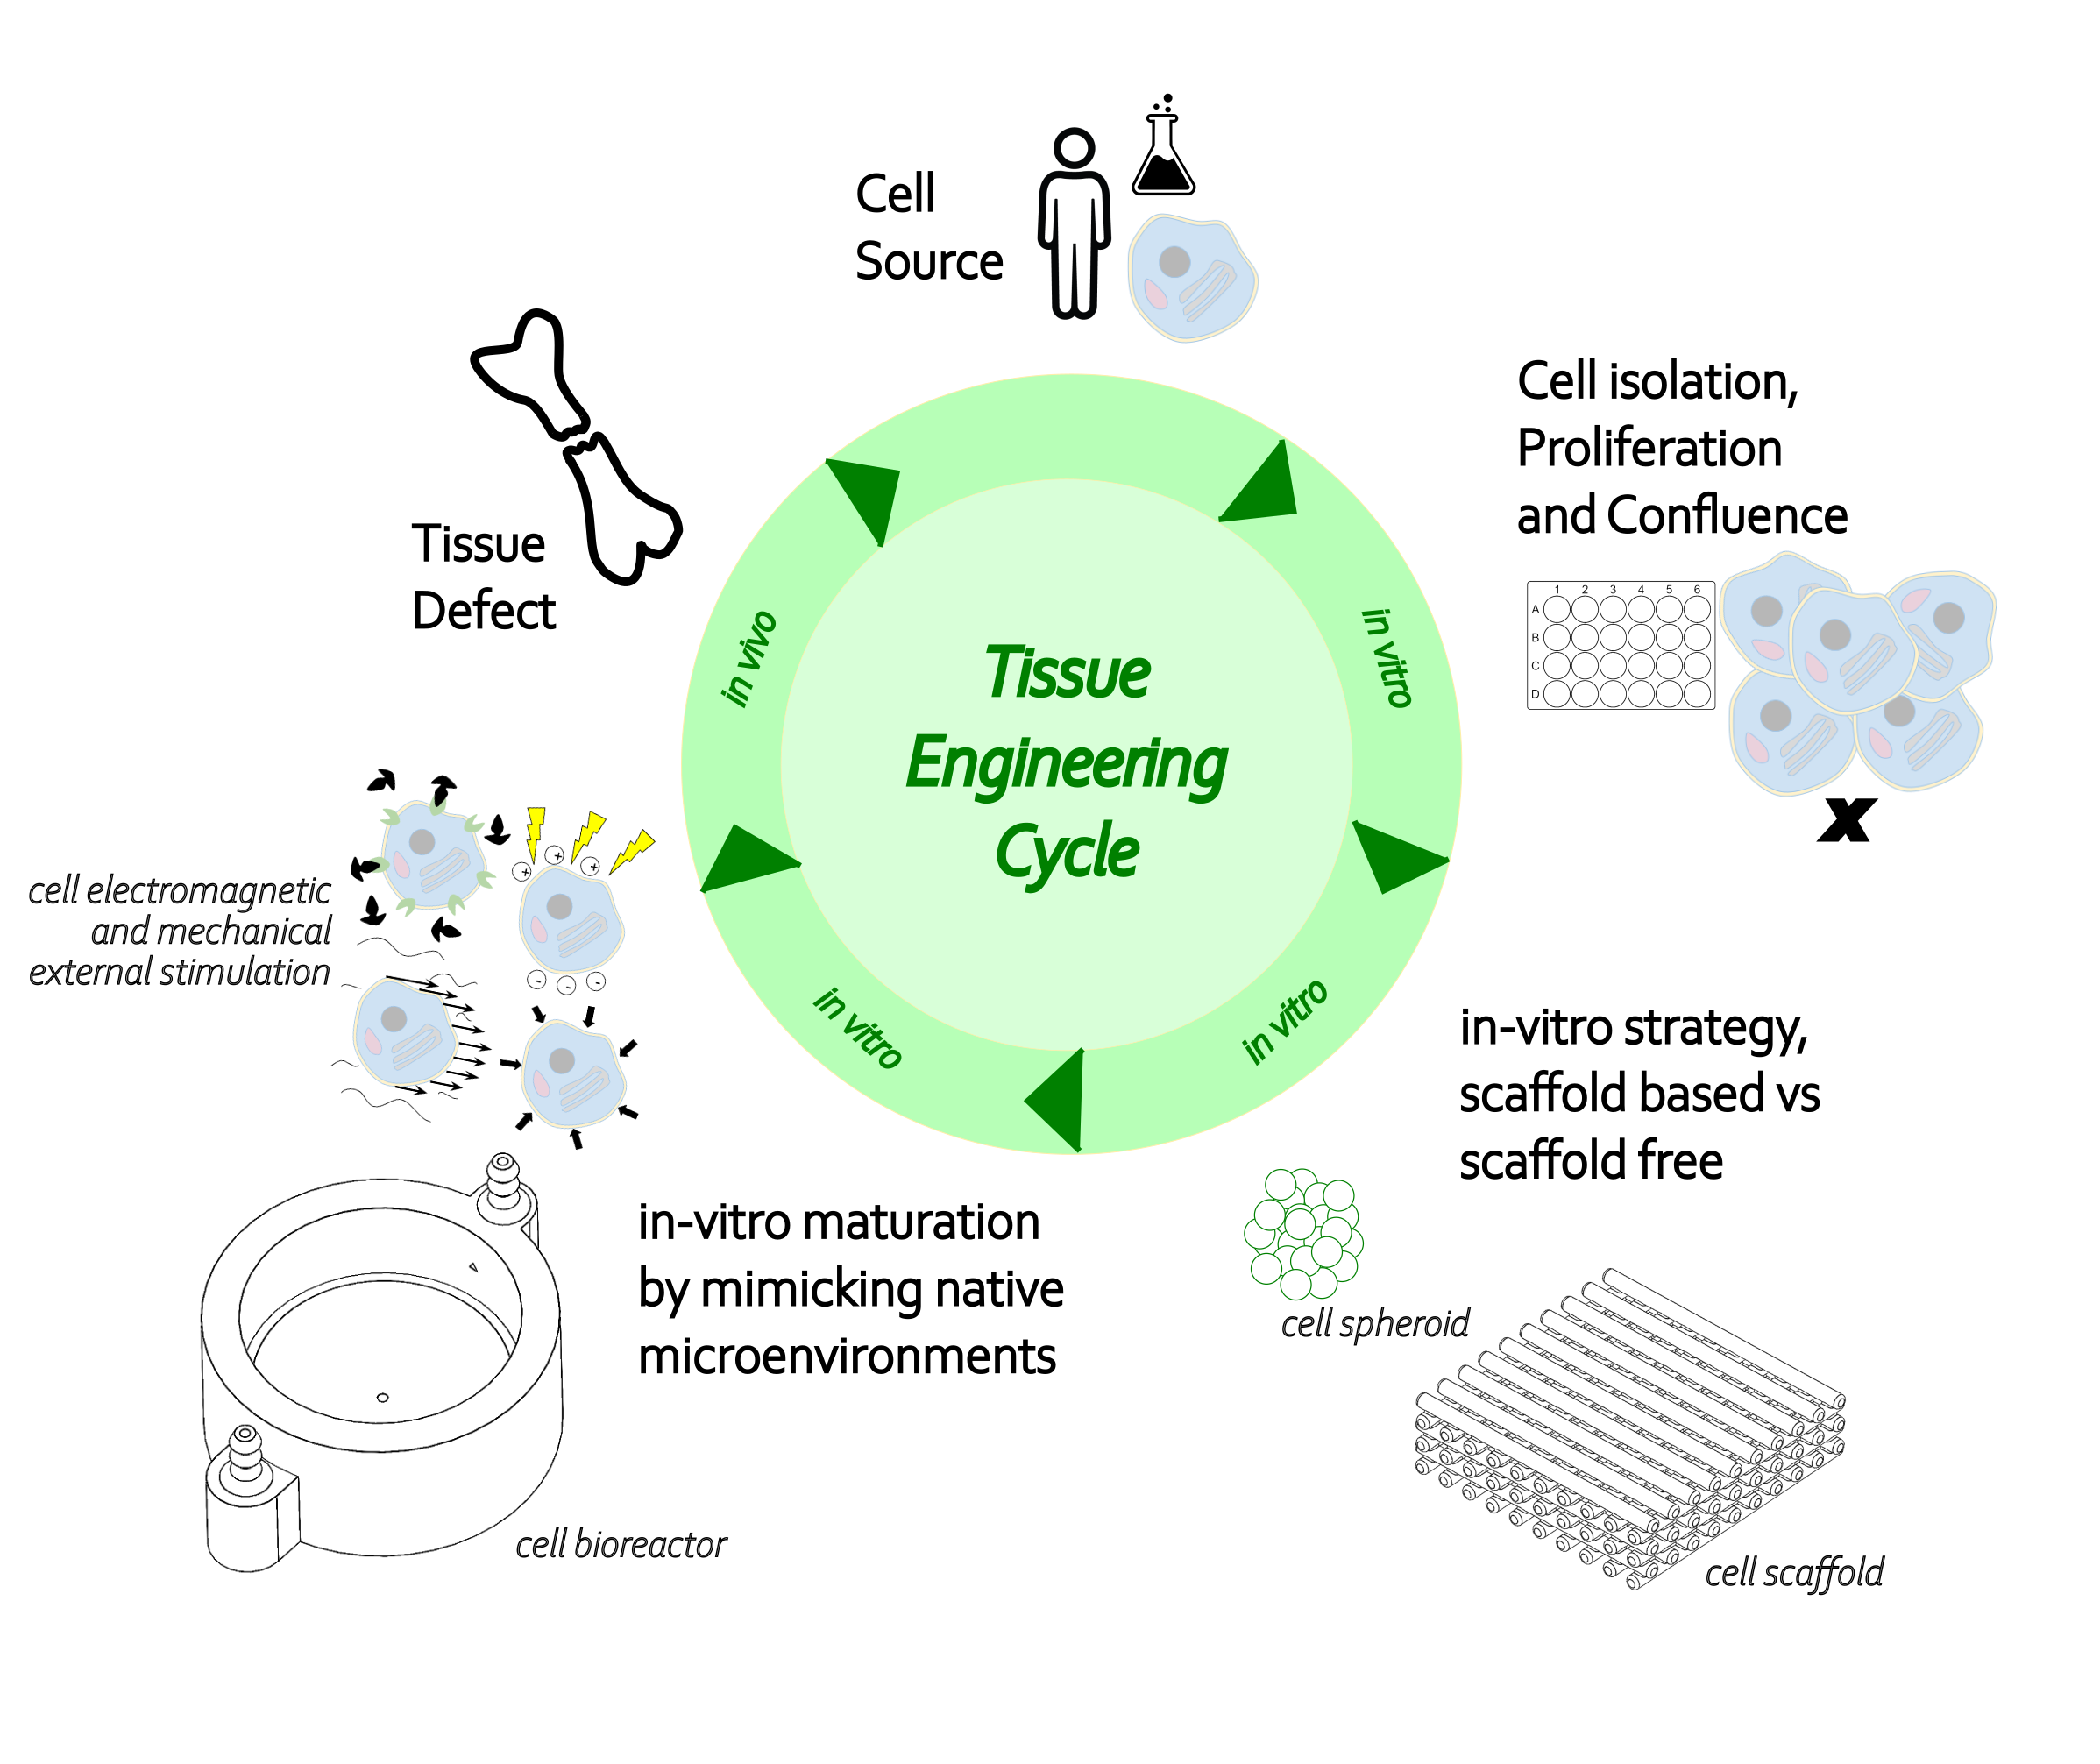
\includegraphics[scale=0.25]{./figures/Figure_1d1.png}}
\caption{The tissue engineering cycle: illustration of the main steps involved.}
\label{fig1d1}
\end{figure}


\subsection{Scaffold-free strategies}

Scaffold-free strategies are characterized by not using cell seeding or adherence within an exogenous material, which will require large cell numbers to secrete even more significant amounts of \ac{ECM} \cite{DuRaine2015-fu}. This bottom-up strategy seeks to produce tissues by mimicking developmental processes following this pattern: cell condensation, cell proliferation, cell differentiation, \ac{ECM} production, and tissue maturation. Scaffold-free approaches account for self-organization or self-assembly events at the cellular level to obtain sheets, spheroids, or tissue strands as building blocks. This strategy's success relies on these building blocks' capacity to secrete a favorable extracellular matrix fusing into larger tissue constructs \cite{Dissanayaka2020-ig}. Cell sheet engineering is one of these scaffold-free techniques where cells are expanded in a monolayer until they achieve a high confluence. Once a cohesive \ac{ECM} layer is obtained, the resultant sheet is lifted and externally manipulated to form the desired structure. Also, multiple sheets can undergo tissue fusion to address more extensive tissue defects \cite{DuRaine2015-fu}. Aggregate tissue engineering is another scaffold-free technique that uses self-organized cell aggregates (cell spheroids) that occur in culture, by applying a rotational force or another non-adherent process to cells in a suspension. Fusing small aggregates to form larger tissues, or injecting aggregates into defects, are considered two of the most promising methods to apply this technique. A recent development is the deposition of cell aggregates in spheroids and strands as cell-only bio-ink to additively fabricate complex \ac{3D} printed constructs \cite{Khoshnood2020-ll}. Another emergent scaffold-free strategy is simultaneously a cell-free strategy. It selectively isolates a set of paracrine molecules and biological factors, collectively termed secretome, due to being secreted by cells into the extracellular space. This strategy suggests that a significant part of cell-based therapeutic benefits are due to their secretome, which may include extracellular vesicles that, after being collected, are applied to the original organ defect impacting many regenerative biological functions \cite{Daneshmandi2020-nn}.


\subsection{Scaffold-based strategies}

Scaffold-based strategies mainly rely on using biomaterials to create a \ac{3D} structural construct with interconnected pores (the scaffold) that support the seeded cells throughout the process of tissue formation \cite{Dissanayaka2020-ig}. The scaffold and the adherent cells are cultured under appropriate biophysical and biochemical conditions for further proliferation and differentiation into the desired tissue \cite{Howard2008-qk}. \textit{In vitro} cell cultures can be made static or dynamic (inside a bioreactor), a culture option that dictates the availability of nutrients and metabolic waste removal according to the profile of the generated culture media fluid flow. When the cultured tissue reaches maturation, a subsequent transplantation phase is performed to address the original \textit{in vivo} health condition. \ac{TE} scaffolds are designed to influence the physical, chemical, and biological environment surrounding a cell population \cite{Reina-Romo2019-ry}. To do so,
scaffold biomaterial(s) are selected accordingly with the cell(s) type and source to promote their adhesion, proliferation, and differentiation. An extensive list of biomaterials and their correspondent cellular interactions has been compiled for a wide range of different cells \cite{Qu2019-qq}, highlighting those that provide improved support and attachment surface, while simultaneously serving as a platform to deliver chemical and physical environmental cues (e.g., growth factors, surface proteins, cellular signals, electrical or mechanical patterns). It is well established that cell function is influenced by scaffolds' composition, topography, and architecture, along with the presence of soluble mediators sculpt the success of scaffold-based strategies \cite{Ripamonti2004-vm}. The adequation of scaffold properties and design to generate the most favorable environment (\textit{in vitro} or \textit{in vivo})  for tissue regeneration is the current critical challenge in scaffold-based strategies \cite{Hutmacher2023-le}.   


\section{Bone tissue engineering}

\ac{BTE} is a subset of tissue engineering dedicated to provide novel methods to treat segmental and contained skeletal defects difficult to repair by conventional strategies. The main idea is to restore the natural signaling pathways of bone development and heal the existing skeletal defects. The standard approach to bone regeneration in \ac{BTE} includes three building blocks: a cellular osteoblastic line that secretes bone matrix (or its progenitor cell line); a scaffold to support cellular attachment and fill the skeletal defect, providing appropriate mechanical stability; bounded systems capable of triggering osteoinduction through the delivery of osteoconductive signals and growth/differentiation factors. Osteogenesis induction of bone progenitor cell lines usually includes dexamethasone, ascorbic acid and sodium-Beta-glycerophosphate to promote differentiation, and \ac{VEGF}, \ac{FGF} or \ac{BMP} to promote growth \cite{Francois2019-ip, Miron2012-vk, Franz-Odendaal2006-eu}. A recent strategy to obtain bone tissues begins with engineering cartilaginous constructs and then attempts to recapitulate the embryonic processes of endochondral ossification \cite{Fu2021-us}.

There is an increasing demand for \ac{BTE} clinical approaches due to the short donor supply of bone substitutes (bone grafts), following the demographic rise of the elderly population. A systematic analysis conducted worldwide (including 204 countries and territories) from 1990 to 2019 concluded that in 2019, there were 178 million new fractures (a 33.4\% increase since 1990), 455 million prevalent cases of acute or long-term symptoms of a fracture (a 70.1\% increase since 1990), that are translated to 25.8 million years lived with disability (a 65.3\% increase since 1990) \cite{Cauley2021-vt}. This data reflects a significant societal and economic cost. In the European Union, the bone fragility fractures in the six founding member states are estimated to increase 23\%, from 2.7 million in 2017 to 3.3 million in 2030 \cite{Borgstrom2020-ki}. These will be further aggravated as the European 'age quake' approaches its historical highest magnitude, going from a median age of 37.7 years old in 2003 to a median age of 52.3 years old by 2050.

Bone fractures may occur after trauma, infection, or oncologic resection. Minor bone defects usually heal without complex interventions, but critical size defects (incapable of spontaneous healing) require one or more surgical procedures to induce union and regeneration \cite{Gordeladze2017-gs}. These surgical interventions involve bone-grafting techniques and other slow healing techniques with autologous or allograft bone that have the disadvantage of regularly producing problems such as fast degradation rates, reduced bioactivity, donor site morbidity, or the risk of pathogen transmission \cite{Peric_Kacarevic2020-hp}. Another drawback of traditional treatments is that there is no guarantee that the applied procedure can completely correct the bone defect. Therefore, searching for surgical alternatives presents a crucial challenge in orthopedic traumatology \cite{Guerado2017-un}.

Anatomically, bone is composed of two distinct regions, one containing dense and solid cortical bone and the other containing honeycomb-like trabecular cortical bone. Cortical bone accounts for 80\% of the total bone mass and performs the major structural function of bone. In terms of mechanical characteristics, cortical bone possesses a compressive strength ranging from 100 to 230 \si{\mega\pascal} and Young’s modulus ranging from 10 to 20 \si{\giga\pascal}, while trabecular bone only reaches 2–12 \si{\mega\pascal} and 0.01–0.9 \si{\giga\pascal}, respectively \cite{Chang2022-ah}. Microscopically, trabecular bone is unorganized and unstructured, while the cortical bone is composed of spatially organized structures, called osteons. These are identified as a hierarchical cylindrical structure surrounding a Haversian canal containing osteocytes, lamellae, and the lacunocanalicular network. The capability of sensing and transducing mechanical stress is attributed to osteon networks, making the bone responsive to external stimuli, moreover, the Haversian canal is known to transport osteoclast and osteoblast progenitor cells to initiate cortical bone remodeling \cite{Chang2022-ah}. Osteocytes are the key regulator of bone turnover \cite{Goldring2015-kn}, mediating osteoclast bone absorption by modulating the RANKL/OPG expression pattern on the plasma membrane and mediating osteoblast bone formation by releasing DKK-1 and sclerostin, two critical inhibitors of the Wnt/b-catenin pathway. Moreover, osteocytes can indirectly participate in bone turnover by secreting bioactive molecules (e.g., prostanoids, nitric oxide, IGF, VEGF, TGF-b), playing critical roles in mechanosensation that is probable to be activated by sensing the bone fluid flow shear stress within the lacunocanalicular network \cite{Murshid2022-rs}. The detailed mechanism of osteocyte mechanotransduction remains a topic under active discussion, trying to make sense of the particular roles of its dendrites, primary cilia, and cell membrane receptor integrins. Nitric oxide, ATP, and prostaglandin have been proposed as signal mediators in this process \cite{Nguyen2013-bx, Geoghegan2019-qi}.

Bone is a composite tissue with organic (mainly made of collagen type I) and inorganic phases (primarily calcium phosphates in the form of \ac{HA}) \cite{Peric_Kacarevic2020-hp}. Regarding cellular content, the most abundant cellular component of mammalian bone cells is osteocytes, approximately 95\% of all bone cells. There are ten times more osteocytes than osteoblasts in an individual bone \cite{Franz-Odendaal2006-eu}. When a critical size fracture occurs, the standard \ac{BTE} approach is to fill the bone defect gap with a scaffold material that should provide characteristics similar to the previously existing native bone structure, such as surface roughness, porosity, pore size interconnectivity, degradation rate, mechanical properties, and biocompatibility. Osteogenesis will occur on the implanted scaffold, depending on its capability to recruit four primary bone cells: bone-lining cells, osteocytes, osteoclasts, and osteoblasts. A significant focus is given to recruiting osteoblasts since their functions include depositing \ac{HA} crystals into the voids between the collagen fibrils, a process called biomineralization. The degree of biomineralization is the characteristic that determines the mechanical properties of a particular bone tissue. Osteoblasts produce new bone and originate from \ac{MSCs} \cite{Franz-Odendaal2006-eu}. \ac{MSCs} may play a significant role in \ac{BTE} strategies due to their capacity for osteogenic differentiation and their abundant availability, since they exist in many organs and tissues of the human body \cite{Guillot-Ferriols2022-wn}. Regarding bone graft substitutes (\ac{BTE} scaffolds), despite the possibility of being made from different materials (e.g., natural or synthetic polymers, bioceramics, metals), they should provide an osteointegrative, osteoinductive, and osteoconductive environment. The osteoinduction process stimulates immature cells (\ac{MSCs}) to develop into preosteoblasts, a process that is typically conducted \textit{in vitro} inside a bioreactor. This mentioned bioreactor unit is one of the central technologies in \ac{BTE} supporting scaffolds and adherent cells, with the increasing mass transport requirements of growing tissues. The bioreactor also allows a controlled recreation of an osteoinductive cellular environment (e.g., chemically, mechanically, electrically), mimicking bone native conditions until the sustained cell culture is sufficiently mature to be transplanted and fill patients' original bone defect.

This thesis research chose \ac{BTE} with the described scaffold-based strategy as a proof of concept due to its growing relevance and the fact that bone cells naturally respond to mechanical and electrical stimulation \cite{Wang2022-op, Nunez-Toldra2020-ai}. This methodological reductionism, from \ac{TE} to \ac{BTE}, is required for practical demonstration and analysis. Even if some conclusions are only valid for the selected cell/tissue type under study, the subjacent developed systems and techniques can be adapted to apply in other \ac{TE} areas without losing their feasibility.


\section{\textit{In-vitro} experimental variability sources}

The final goal of \ac{BTE} is to repair the patient's bone defect. The success of \ac{BTE} strategies crucially depends on the final \textit{in vivo} reimplantation phase, which conceals many unknown uncertainties in the complex biochemical and biophysical interactions between the implant and target tissues. To achieve a successful \ac{BTE} strategy, one must first make sense of the previous \textit{in vitro} cell culture phase before moving on to implantation. It is known that the state-of-the-art in \ac{BTE} \textit{in vitro} research presents a core problem: high research variability in experimental settings and outcomes. This variability lowers reproducibility and narrows the application of \ac{BTE} outputs into everyday practice. This subchapter focuses on identifying the primary sources of variability in \ac{BTE} research. This is an essential step to determine how \textit{in vitro} outcomes can be controlled to increase reproducibility and finally address the remaining challenges of the \textit{in vivo} phase.

\subsection{Bioreactors, flow regimes, and scaffolds}

To bioengineer a bone graft, it is required to pick an adequate cell source and seed the selected cells in an adequate number into the cell support structure, while at the same time providing all the appropriate \textit{in vitro} cell culture conditions to achieve significant levels of proliferation and differentiation. Many systems have been developed and applied in \ac{BTE} over the years to obtain the living bone grafts described above. Nevertheless, it is the presence of two standard non-biological systems that directly support cell culture: a bioreactor system (see Figure \ref{fig1d2}), defined by the vessel that contains the cell culture, responsible for the control and actuation processes, efficiently performing cell nutrient support, cell waste removal and temperature stabilization; a scaffold system, composed of the biomaterial that provides structural support and a tridimensional orientation for cells to migrate and grow, mimicking \ac{ECM} functions. 

\begin{figure}
\makebox[\textwidth][c]{\includegraphics[scale=0.07]{./figures/Figure_1d2.png}}
\caption{Standard non-biological systems that directly support cell culture are shown to exemplify the diversity of systems that need to be accounted for. Shown bioreactor systems differ in operation, design, and level of automation, constituting a source of \textit{in vitro} experimental variability. Additionally and independently from the bioreactor chosen, multiple cell culture options (listed in the image's top left corner) will impact the cell culture results. All bioreactors present in the figure are perfusion bioreactors adapted from the literature \cite{Lim2019-gx, Birru2018-rj, Gabetti2022-hp}.}
\label{fig1d2}
\end{figure}

Bioreactor technologies in \ac{BTE} can be divided into three categories: perfusion bioreactors, rotating bioreactors, and spinner flask bioreactors \cite{Kazimierczak2022-mq}. Vessel design, construction techniques, and mode of operation pose significant differences between these categories \cite{Melo-Fonseca2023-fd}. Differences also appear when comparing systems inside the same category. Computational modelling studies of media flow in \ac{BTE} reactors revealed different fluid velocity profiles that induce a significant variation in shear stress distribution when comparing results between perfusion with rotating \ac{BTE} bioreactors \cite{Nokhbatolfoghahaei2020-yt}. Since different levels of shear stress are expected to generate different cellular outcomes, bioreactor-dependent velocity profiles constitute an important source of experimental variability. 

Calling for best practices in mammalian cell culture environmental control is becoming prominent \cite{Klein2021-dz, Klein2022-yj}.  Even slight deviations in mammalian cell culture from the physiological levels, regarding \acs{pH} \cite{Michl2019-js} or dissolved gasses (\acs{dO2}, \acs{dCO2}) \cite{Ast2019-mc, Place2017-bn}, can provoke substantial cellular perturbations. This, in turn, can profoundly impact study conclusions when these conditions are incorrectly assumed to be stable, or when a critical biological parameter for reproducibility is ignored and routinely not measured or incorrectly reported \cite{Al-Ani2018-df}. The evolution of bioreactor systems to improve upon these best control practices is critical to increase the understanding of experimental results in \ac{BTE}.

Performing cell cultures on tissue-engineered scaffold structures adds a new group of variability sources. The specific interactions between the seeded cells and the introduced biomaterial structural and physical attributes became relevant to consider \cite{Zaeri2022-wk}. For instance, the presence of a scaffold in the cell culture chamber contributes to different nutrient flow and diffusion patterns emerging from its geometry interference \cite{Woo_Jung2013-yq}. The scaffold fabrication process also plays a role in introducing variability, adding specific limitations and outcomes influenced by the fabrication process itself. For example, scaffolds produced by rapid prototyping techniques show architecture variations compared to the original \ac{CAD} design and intersample variability, when compared to other scaffolds produced by the same fabrication process \cite{Campos_Marin2015-qc}. Computer fluid models were performed on additive-manufactured scaffolds reconstructed by \ac{mCT}. Those \ac{mCT} modelling results revealed different fluid velocity and \ac{WSS} profile patterns, showing higher values and more irregular profiles when compared to the precursor \ac{CAD} model analysis. Also, from sample to sample, different \ac{WSS} patterns emerged. These variations affect local fluid velocities and \ac{WSS} values, affecting each cell's mechanical microenvironment and becoming a noise source for \textit{in vitro} experiments. In the worst-case scenario, they may result in heterogeneous cell distributions and different cell responses throughout the scaffold. Scaffold inspection/verification processes based on \ac{mCT} reconstructions have been proposed to become a standard practice to understand the impact of manufacturing limitations on scaffold geometry and consequent biological performance \cite{Podshivalov2013-sy}. 

\subsection{Cell sources and cell culture options}

From static to dynamic cell cultures, with or without cell support structures, a documented important source of variability are the options adopted regarding cell source and cell culture process. Different cell types or even the same cell type from different origin tissues or cellular phases have different metabolic needs that, without proper care, can deplete the culture medium of nutrients \cite{Al-Ani2018-df}. Oxygen consumption ratios, cell seeding density, experiment duration, culture vessel geometry, and media volume all interplay to influence cell nutrient availability, impacting cell culture outcomes. This is even more complex if we consider, for example, that a  proper oxygen delivery must account for additional parameters affecting solubility like temperature variations, atmospheric partial pressure, humidity, carbon dioxide concentration, convective mixing systems, and the ionic strength of culture media, all affecting the amount of oxygen available to cells at each moment. Also, practices for handling the tissue culture should be carefully considered since the number of times they are handled, and the handling procedure exposes the cell culture to different gas mixtures, causing changes in the oxygen concentration in the culture media. Those changes may provoke an imbalance that can take hours to reach a new equilibrium steady state.

Focusing on cell growth and avoiding apoptosis, good cell culture media selection allows controlling osmolality, ammonia levels, and the production of free radicals \cite{Price2017-mm}. For optimal results, researchers need to know the best physical parameters of the cells intended to be cultured. Those will allow supplying: an adequate balanced salt solution in terms of concentrations of anions (e.g., PO\textsubscript{4}\textsuperscript{3-}, Cl\textsuperscript{-}, HCO\textsubscript{3}\textsuperscript{-}) and cations (i.e. Na\textsuperscript{+}, K\textsuperscript{+}, Ca\textsuperscript{2+}, Mg\textsuperscript{2+}); proper levels of energy sources (i.e. glucose and glutamine), vitamins, essential and nonessential amino acids, lipids. The optimal choice of medium depends on the target cells and the purpose of the research. Choosing between classical formulations with serum, serum-free options, or chemically defined media has advantages and disadvantages. Insufficient nutrients or excess toxic byproducts will profoundly impact cell culture results. A significant cause of lack of reproducibility in \ac{TE} applications is the poor implementation of quality control measures and reporting standards. For this reason, good cell culture practices and guidelines for every process step are constantly being updated and revised \cite{Pamies2018-fm, Geraghty2014-rb, Pamies2022-cq}.

\subsection{External stimulation technologies and protocol options}

Mechanical and electromagnetic stimuli have been routinely added to the existing cell culture conditions through specially designed external stimulation systems to lead cells into improved proliferation or/and differentiation or to mimic native tissue conditions where they naturally exist.  

In BTE, fracture healing is a complex, multistep process susceptible to mechanical signaling and micro-mechanical cues \cite{Anani2022-vm}. External mechanical stimulation systems vary in their core technology; by doing so, they all deliver mechanical stimuli with slightly different characteristics. The use of low-intensity pulsed ultrasound, for example, applies an oscillating longitudinal pressure wave with a frequency generally greater than 20 kHz \cite{Harrison2021-gy}. Other techniques use a constant or sinusoidal applied hydrostatic pressure (waveform from 0.001 to 2 Hz) \cite{Henstock2013-co, Nesler2016-le, Stavenschi2018-ze}, whose magnitude is reported to vary between 0 and 300 kPa. More standard methods to apply mechanical stimuli involve direct compression/elongation of the scaffold structure or resorting to perfusion interactions, like fluid flow-induced wall shear stress, to transmit forces to the seeded cell region \cite{Wittkowske2016-xr}. This multitude of methodologies resulted in a significant number of designs that can be generally categorized as fluid perfusion systems, rotary devices (e.g., spinner flasks), dynamic compression/tension systems, vibrational and hydrostatic pressure chambers \cite{McCoy2010-hy, Sart2016-uq, Campsie2019-jq}. These different systems and their multiple protocols introduce specific differences in the cellular microenvironment generated by mechanical stimulation and consequent mechanotransduction effects. This hinders the comparison among results to retrieve solid conclusions \cite{Sun2022-xt}.

Electromagnetic field stimulation in BTE has been shown to promote different ranges of cellular response, from proliferation, migration, growth, differentiation, extracellular matrix expression, or even apoptosis \cite{Thrivikraman2018-su}. Electric fields (\acs{EFs}) are thought to transiently change membrane polarization and permeability of specific ion channels, modulating cascades of events at the intracellular level \cite{Bhavsar2019-iz}. The application of an electromagnetic field consists of a non-specific process that targets any charged particle. Thus, various cellular processes may be modulated by \acs{EFs} with different characteristics (e.g., different magnitudes and frequencies). Experimental setups that apply electromagnetic fields are commonly classified into three groups \cite{Thrivikraman2018-su, Balint2013-rd, Nicksic2022-jy}: 

\begin{itemize}
\item \ac{CCoupled} systems - these apply a time-varying electric field, with both setup electrodes separated from the cell culture medium by an electric insulator layer. A less used variant is the Semi-Capacitively Coupled system, where one of the electrodes is in direct contact with the cell culture medium while the other remains electrically insulated;

\item \ac{DCoupled} systems - a steady or time-varying electric field is applied, with both setup electrodes in contact with the cell culture medium (immersed), or separated from the cell culture medium by an agar-salt bridge;

\item \ac{ICoupled} systems - the setup usually comprises Helmholtz coils that apply a time-varying magnetic field, producing an induced electric field in the cell culture medium region (electromagnetic induction).
\end{itemize}

\ac{ICoupled} systems contrast with the other groups because they apply electromagnetic stimulation by delivering superimposed electric and magnetic fields. An exception can be made to \ac{ICoupled} applications like the transformer-like coupling method, which allows to isolate cellular effects due only to an \ac{EF} \cite{Hess2012-kw}. Even though \ac{CCoupled} setups had less expression in recent publications relative to \ac{DCoupled} and \ac{ICoupled} configurations, this kind of setup offers some advantages when trying to minimize experimental variability. First, \ac{CCoupled} electrodes are not in direct contact with the culture medium, contributing to block electron transfer to the culture medium, avoiding the formation of oxidative radicals species (faradaic products), usually present in \ac{DCoupled} setups, and whom may influence cellular response and survival \cite{Srirussamee2021-cj}. Second, \ac{CCoupled} devices allow to isolate the effects of the \acs{EFs} without additional chemical artifacts, a feature also achievable in ICoupled setups, but with no distinction between actions of electric and magnetic fields. Besides the technology differences, high protocol dissonance can be observed and is extensively compiled in literature reviews \cite{Kim2015-vg, Ryan2021-tq, Da_Silva2020-su, Thrivikraman2018-su}. The mentioned reviews state that difficulties in concluding electrical stimulation studies mainly arise from the varying values of applied stimulation strength or other differences in stimulation protocols, aggravated by incomplete device specification. Thus, it is recommended to increase scientific rigor and report a novel minimum set of parameters \cite{Nicksic2022-jy}.
 
Figure \ref{fig: F3} establishes a visual comparison between a sample of protocols applied in \ac{DCoupled} \acs{EFs} stimulation to exemplify the substantial variability between different experimental studies, even when considering the same external stimulation technology and cellular line.

\begin{figure}
\makebox[\textwidth][c]{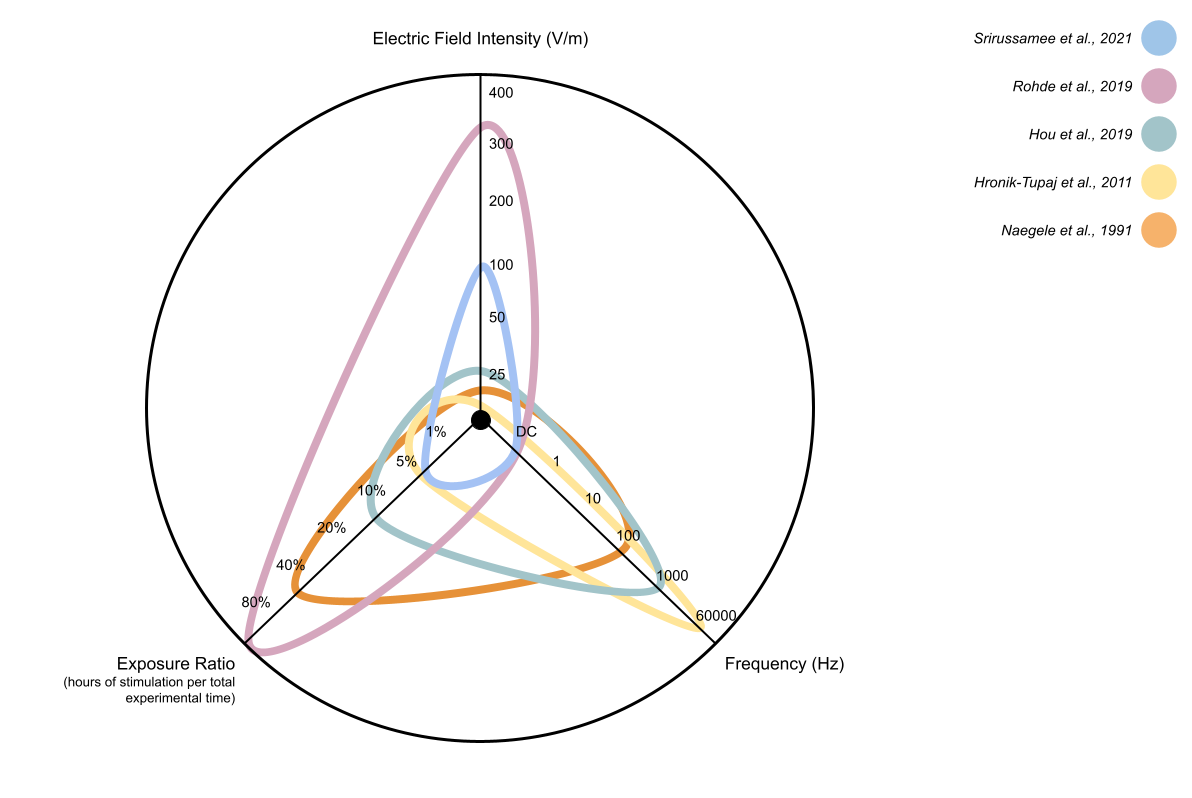
\includegraphics[scale=0.4]{./figures/Figure_1d3.png}}
\caption{Protocol design variability in electromagnetic field stimulation parameters, considering five different \ac{DCoupled} \acs{EFs} studies \cite{Srirussamee2021-cj, Hou2019-yd, Hronik-Tupaj2011-cx, Zhao2011-wy}.}
\label{fig: F3}
\end{figure} 


\section{Context of the thesis}

In TE and BTE, bioreactor and scaffold design are of paramount importance to promote and sustain adequate \textit{in vitro} conditions for cell culture differentiation, proliferation, growth, and support. In addition to nutrient transport and waste removal, diverse bioreactor designs have been developed to provide mechanical or electromagnetic stimuli to cells, enhancing physical microenvironmental conditions to unlock specific cell responses. Previous studies have shown that single or combined stimuli significantly upregulate important cellular functions related to regenerative processes. For different stimulation types and cellular tissues, adequate stimulation properties have been experimentally determined and reported in several \textit{in vitro} studies. However, the biophysical mechanisms by which cells sense, interpret, and transform these stimuli into actions remain unclear. Even under the same cellular lines, experimental protocols present a high variability (quantitative and qualitative) of stimulation parameters and also on the geometry and materials of the setup used for applying the intended stimuli. Reported results of diverse stimuli application prove to have beneficial effects in cell cultures. Still, their protocol design variability originates questions regarding the most appropriate and relevant stimulation parameters and which effects are being effectively produced and observed \cite{Thrivikraman2018-su}.

This Ph.D. thesis aims to develop a multimodal stimulation all-in-one bioreactor design strategy attempting to combine electromagnetic and mechanical stimulation under a common open-source platform. This concept includes sensors for online monitoring and control units to fully automate the bioreactor system. The process of designing the intended bioreactor also includes scaffold design stages, both of them guided by their digital model (an accurate virtual numerical model constructed to reflect the physical object). These constructed numerical models allow us to precisely predict the delivered biophysical microenvironment, a piece of information useful to optimize the bioreactor and scaffold in the design phase. These models are also useful to redefine stimulation protocol standards for bone cell stimulation, fine-tuning the stimulation to better test and provoke cellular responses. Additionally, this thesis proposes a data-driven design methodology based on numerical model predictions, to better understand the underlying biophysics of external stimulation systems and the impact of adding scaffold structures to the cell culture chamber in stimulation-induced outcomes. Despite making the analysis in the subset of \ac{BTE}, most of the conclusions can be easily transferred to other tissues, opening new perspectives for stimulation systems in \ac{TE}. An open-science commitment is made in this thesis, through sharing of detailed methodologies and results in open-source public repositories. This contributes to increase shareability, reproducibility, and standardization of \textit{in vitro} stimulation and culture experimental procedures among researchers.

\subsection{Thesis overview}
This thesis is organized as follows:
\begin{itemize}
\item Chapter 1: Introduction;
\item Chapter 2: Numerical models of external stimulation methods;
\item Chapter 3: Numerical modelling of mechanical stimulation;
\item Chapter 4: Numerical modelling of direct-coupled electric field stimulation;
\item Chapter 5: Numerical modelling of capacitive-coupled electric field stimulation;
\item Chapter 6: All-in-one bioreactor design methodology driven by numerical model predictions;
\item Chapter 7: Final considerations;
\item Chapter 8: Scientific outputs.
\end{itemize}


%\newpage
%\bibliography{library_c1} 
%\bibliographystyle{plain}
%\end{document}
%\documentclass[11pt]{report}
%\usepackage{siunitx}
%\usepackage{graphicx}

%\begin{document}
%\setcounter{chapter}{1}
%\tableofcontents


\newpage
\chapter{External stimulation methods, its effects and models}
This chapter delves into numerical models of external stimulation methods. Capacitive-coupled and direct-coupled external stimulation methods were considered for electric field stimulation delivery, while fluid flow-induced shear stress was considered for mechanical stimulation delivery. Reported biological effects and transducer pathways triggered by each stimulation method are also described. Finally, this chapter includes a state-of-the-art concise review on reported approaches for numerical modelling of each external stimulation method, including some case studies. 



\newpage
\section{Mechanical systems}
Several mechanical stimulation strategies have been developed in \ac{BTE} to overcome inhomogeneous cell distribution and suboptimal differentiation outcomes. In addition, these strategies aimed at accelerating bone formation processes \cite{Melke2018-kv}. Among the various developed mechanical stimulation setups \cite{Melo-Fonseca2023-fd}, fluid perfusion setups were selected for this thesis work, since these apply mechanical stimulation through fluid flow-induced wall shear stress while simultaneously performing mass transfer of nutrients and removal of cell metabolic waste. This is an advantage over other mechanical stimulation technologies operating on static cultures or closed containers without continuous culture medium replacement. This section enumerates the observed biological effects and proven underlying mechanisms for fluid flow-induced shear stress application for multiple cell lines. Literature-reported strategies for numerical modelling these mechanical setups are also discussed. 


\subsection{Fluid flow-induced shear stress setups}


\subsubsection{Reported biophysical effects}
Two categories of setups commonly apply flow-induced shear stress stimulation: the ones that generate a perfusion fluid flow \cite{McCoy2012-jv} and others that generate rotating fluid media (e.g., spinner flask, stirred tank bioreactor, rotating-wall vessel) \cite{Melke2018-kv}. Although both define specific ranges of wall shear stress, these also create dynamic conditions that are dependent on the fluid flow profile generated and pre-conditioned by several physical conditions (fluid velocity, turbulence, channel design, number of inlets and outlets, inserted scaffold design, etc.). If improperly planned and applied, they may result in cell detachment, damage, and apoptosis. Several setups for fluid-induced shear stress stimulation of cell-scaffold constructs have been developed over the years \cite{Alvarez-Barreto2011-lj, Filipowska2016-cd, Gardel2013-cs, Jaasma2008-oe}. Many differ significantly in design and protocol, which hinders precise comparisons and well-sustained identification of the effects of this type of mechanical stimulation in cells.

Biomechanical studies have demonstrated that more than 90\% of bone cells within the \ac{ECM} are osteocytes. These cells sense and transduce mechanical forces exerted on the bone, governing the rates of mineral resorption and deposition that occur during bone remodeling \cite{Franz-Odendaal2006-eu}. Mechanical stimulation applied to osteocytic networks under steady or oscillatory perfusion flow \cite{Lu2012-vh} is observed to modulate intracellular Ca\textsuperscript{2+} responses, specifically the calcium peak's magnitude and frequency, which vary with the fluid flow profiles. Effects of mechanical stimulation on \ac{MSCs} and their surrounding microenvironment were reviewed by Sun et al. \cite{Sun2022-xt}: mechanotransduction occurs via integrins and mechanosensitive ion channels that transmit the mechanical signals via actin stress fibers and known molecular pathways (e.g., RhoA, MAPK, Vinculin, Talin, ERK, YAP/TAZ). Interestingly, some stretch-activated channels mediate intracellular Ca\textsuperscript{2+} responses upon mechanical stimulation \cite{Walker2000-bc, Luo2013-wv}, an effect also showed to be induced by \acs{AC} electric fields in this type of channels in the absence of mechanical stimulation \cite{Cho1999-hr}, which indicates the potential for these channels to be modulated for both kinds of biophysical stimulation. Also, the Wnt signaling pathway was observed to be an essential control mechanism in bone response to mechanical loading \cite{Choi2021-jk}. \ac{MSCs}, when subjected to fluid flow-induced wall shear stress, showed an increase in cell attachment, spreading, cell viability, and osteogenic differentiation \cite{De_Luca2020-hp}. This is transduced in the expression of early markers of osteogenic differentiation like \acs{RUNX2}, \ac{ALP}, and osteopontin or \ac{SPP1}, as well as increased mineralization, comparatively to a static culture. The mechanical environment of bone is complex, and it remains unclear how precisely macro-scale mechanical actions will translate into micro-scale events that regulate and affect bone precursor cell differentiation. Nevertheless, mechanical stimulation has been shown to promote bone growth, improving mineralization and secretion of many specialized extracellular matrix proteomes, such as type I collagen \cite{Partap2010-xt}.


\subsubsection{Reported numerical modelling techniques}
Numerically modelling perfusion setups with or without porous scaffolds requires virtualizing their physical structures. This step can be accomplished in multiple ways, either by drawing their equivalent \ac{CAD} geometries or by obtaining their physical structure from image acquisition techniques (e.g., \ac{mCT}), followed by a subsequent tridimensional reconstruction. Fluid flow modelling is usually obtained by solving continuity and \ac{3D} Navier Stokes equations on these complex geometries. If the scaffold is present, no-slip wall conditions are considered for all physical boundaries, including the scaffold surface. The culture medium is modeled as an incompressible Newtonian fluid, and the solution to all this set of equations is obtained by computational methods, namely by \ac{FEM} \cite{Campos_Marin2018-ff, McCoy2012-jv, Vis2023-xt} or by the \ac{FVM} \cite{De_Wildt2023-ev}. When the geometry of the scaffold's porosity is unknown, it is expected to introduce a new set of equations that account for a global permeability, as determined by Darcy's law \cite{De_Wildt2023-ev}. Empirical models have also been developed to calculate the fluid-induced wall shear stress \cite{Ahmed2023-es}, offering an alternative to the solution obtained from \ac{CFD} techniques that use the resultant shear rate and the fluid kinematic viscosity to perform that calculation. In Chapter 3, \ac{CFD} techniques are used to understand the impact of bioreactor design changes in delivering fluid-induced shear stress to the cultured cells region.



\section{Electromagnetic systems}
The two most important communicating systems in the human body, affecting cellular functions, are the nervous and hormonal systems. These two systems act mainly on the cell's membranes to induce endogenous \ac{EF}s that modulate interactions between intracellular and extracellular environments. As macroscopic functions of the body have been reported to be affected by an applied external electric field, it is straightforward to hypothesize that cellular membrane signal transduction mechanisms can be modulated by an applied \ac{EF} of specific strength and form \cite{Seegers2001-jo}.

Multiple experimental setups have been developed and applied to deliver electromagnetic stimulation to \textit{in vitro} cell cultures in \ac{BTE}. A significant number of reviews split electromagnetic applying experimental setups into a subset of technologies, according to the different aspects of how they obtain the electric and/or magnetic field that will exert an effect on the cell culture \cite{Thrivikraman2018-su, Funk2009-is}. As was presented in the previous chapter, \ac{DCoupled} and \ac{CCoupled} systems were selected for further analysis in this work due to their capability to apply isolated \ac{EF}s. The treatment of \textit{in vitro} cell cultures with \ac{EF}s can evoke biochemical and physiological responses that can be favorable to \ac{BTE} outcomes, provided that the stimulation parameters (e.g., waveform signal, exposure duration, field strength, frequency) are within tolerance limits for the exposed cellular type. Despite multiple evidence of the biological effects produced by cell culture exposure to an \ac{EF}, the complete mechanism of this interaction remains unknown, strongly limiting the accuracy of the applications of \ac{EFs} based therapies \cite{Taghian2015-hf}.

\textit{In vitro} and \textit{in vivo} reports commonly attribute the observed \ac{EF} effects to the activation of membrane proteins, specifically proteins involved in signal-transduction mechanisms. Particularly, the concentration of free cytosolic Ca\textsuperscript{2+} is observed to follow the electric stimulation of cells, contributing to activate a cascade of calcium-dependent cellular processes \cite{Pall2013-wt, De_Menorval2016-fv, Brighton2001-fk, Burke2017-su, Cho1999-hr} including cellular motility \cite{Onuma1988-eu}, redistribution of integral membrane proteins and reorganization of microfilament structures \cite{Cho1999-hr}. The oscillation of intracellular free cytosolic calcium concentration is significant for cell signaling and is reported to be impacted by electromagnetic stimulation \cite{Sun2007-tx}. This oscillation is a complex dynamical process and reflects calcium transportation to and from the exterior cell, cytosol, intracellular stores, exchange between cells, or diffusion and buffering due to its binding to proteins. According to Sun et al. \cite{Sun2007-tx}, regulating calcium oscillation by external physical stimulation could amplify \ac{MSCs} differentiation into a tissue-specific lineage and may offer alternative biotechnology to harness the unique properties of stem cells. Osteogenic markers impacted by electromagnetic stimulation include the expression of \acs{ALP}, \acs{COL1}, osteocalcin and osteopontin, BMP-2, DCN, \acs{RUNX2}, MAPK, ERK, p38 \cite{Guillot-Ferriols2022-wn}. An extensive list of osteogenic differentiation regulatory agents was compiled by Deng et al. \cite{Deng2008-xs}, and a review of the positive and negative effects of electromagnetic stimulation in stem cells is given by Maziarz \textit{et al.} \cite{Maziarz2016-fd}. This section enumerates the observed biological effects and underlying mechanisms for \ac{DCoupled} and \ac{CCoupled} systems. It also discusses the impact of different \ac{EF} patterns applied by both systems in specific cellular responses and how particular setup characteristics contribute to this impact \cite{Meng2021-qn}.


\subsection{Direct-coupled setups}


\subsubsection{Reported biophysical effects}
\textit{In vitro} \ac{DCoupled} electric field stimulation is applied through electrodes immersed in a culture medium, or using a conductive surface/scaffold or Agar-salt bridges \cite{Meng2013-mz}. Direct-current (\acs{DC}) signals are one of the most applied, being current or voltage-controlled. Other studies apply alternate-current (\acs{AC}) or pulsed signals to charge-balance the culture medium, mitigating one of the DCoupled drawbacks, which is a rising gradient in ion distribution in the culture medium that results in altered cell physiology, thus making it difficult to distinguish the effects occurring due to electric field stimulation \cite{Meng2021-qn}. Although variable in the magnitude, frequency, exposure, and waveform, \ac{DCoupled} \ac{EF} stimulation has sequentially proven to modulate different phases of the cell cycle and their metabolic processes, impacting cell proliferation, morphology, and differentiation. 

When subjected to \ac{DCoupled} stimulation, \acs{MSCs} proliferation and osteogenic differentiation occur, accompanied by cell membrane potential changes, with membrane depolarization corresponding to the proliferative phase and membrane hyperpolarization corresponding to the differentiative phase \cite{Bhavsar2019-iz}. Modulation of \acs{MSCs} biomechanics through electrical influence on the cytoskeleton elasticity was observed by Titushkin \textit{et al.} \cite{Titushkin2009-gi}, where elasticity was reduced due to substantial actin reorganization and led to changes in specific linker proteins (ezrin/radixin/moesin family) at focal adhesion sites. These morphological modifications are hypothesized to be connected to the control of cell differentiation and other cellular processes that can, by this way, become efficiently regulated by a \acs{DCoupled} electrical stimulus.

Osteoblast-like cells subjected to \acs{DCoupled} stimulation \cite{Wang1998-ek} increased their proliferation and the presence of calcification deposits. Intracellular free calcium ion concentration was measured, showing an average increase of 2.3 times the initial level. This intracellular calcium ion concentration effect was also observed in \ac{MSCs} cultured in silk scaffold \cite{Cakmak2016-oj} and in conductive scaffolds \cite{Zhang2016-ul} when subjected to a \acs{DCoupled} stimulation. Also, \acs{MSCs} seeded into conductive scaffolds subjected to \acs{DCoupled} stimulation together with blockers of voltage-gated calcium (Ca\textsuperscript{2+}\textsubscript{v}), sodium (Na\textsuperscript{+}\textsubscript{v}), potassium (K\textsuperscript{+}\textsubscript{v}), or chloride (Cl\textsuperscript{-}\textsubscript{v}) channels, showed stimulation reduced effects with the presence of Na\textsuperscript{+}\textsubscript{v}, K\textsuperscript{+}\textsubscript{v}, or Cl\textsuperscript{-}\textsubscript{v} blockers and completely nullified effects with Ca\textsuperscript{2+}\textsubscript{v} blocker. These results indicate that ion fluxes through these channels are promoted by \acs{DCoupled} stimulation and that Ca\textsuperscript{2+}\textsubscript{v} channels play a more critical role than the other three tested channels \cite{Zhang2016-ul}. Another study \cite{Kim2009-dv} reports that applying \acs{DCoupled} stimulation through a biphasic waveform to \acs{MSCs} increased proliferation, alkaline phosphatase activity, calcium deposition, vascular endothelial growth factor and
BMP-2 production. Treatment with selective inhibitors of p38, MAPK, or ERK, as well as calcium channel blockers, reduced the increase
of vascular endothelial growth factor expression and cell proliferation. Kim \textit{et al.} \cite{Kim2009-dv} point that osteoblast differentiation of hMSCs occurs by enhancement of cell proliferation and modulation of the local endocrine environment through \ac{VEGF} and BMP-2, inducing the activation of MAPK (ERK and p38) and the calcium channel.

Studies that applied electric fields in \ac{BTE} research throughout \ac{DCoupled} setups report positive effects for a broad range of \ac{EF} magnitudes, as shown in Figure \ref{fig: F2d1}. Despite the considerable applicability of \ac{DCoupled} stimulation as a tool to improve \ac{BTE} solutions, a systematic study of the impact of the \ac{EF}, with an improved understanding of underlying biochemical mechanisms that are activated, is still missing to optimize its application outcomes. \ac{DCoupled} electric fields were observed to influence different phases of the cellular cycle, from differentiation to proliferation and maturation in terms of late-stage gene expression and development of osteogenic-phenotype properties. However, depending on the type of metals used in \ac{DCoupled} systems' electrodes, an irreversible metal dissolution might occur, modifying the \ac{pH} value of the medium, an undesired effect that may go along with electrode corrosion provoking cytotoxic effects. Faradaic by-products resulting from redox and electrochemical reactions at the electrode-electrolyte interface (carbon reactions, water chemistry interactions) can mislead the results from the application of \ac{EF}s, unless a profound characterization of the electrode-electrolyte interface environment is taken into consideration \cite{Spadaro1982-af}. \ac{DCoupled} systems using salt bridges successfully circumvent this limitation, but present other disadvantages related to the small area of charge delivery, the presence of cell diffusion effects due to concentration differences between bridge contents and culture medium, and difficulties in running several chambers simultaneously while maintaining a stable reaction rate \cite{Guette-Marquet2021-rp}.


\begin{figure}
\makebox[\textwidth][c]{\includegraphics[scale=0.3]{./figures/Figure_2d1.png}}
\caption{A sample of reported electric field magnitudes and biological effects for the same exposed cell type (hMSCs) in different Dcoupled (green) and CCoupled (red) systems.}
\label{fig: F2d1}
\end{figure}
      

\subsubsection{Reported numerical modelling techniques}
Experimentally obtained \ac{DCoupled} \ac{EF} ranges that promote specific cellular processes may be found for several cell types and metabolic phases. Still, the diversity of applied protocols and system options prevents an effective comparison and the drawing of global conclusions. Numerical modelling techniques have been introduced to \ac{DCoupled} systems to help to understand and control the effective magnitude of \ac{EF} stimulation being applied and to get hints on the most probable intracellular targets of a particular stimulation protocol. 

Approaches found in the literature use analytical estimates to predict the \ac{EF} magnitude delivered by DCoupled systems. These divide the applied potential by the distance between the electrodes \cite{Mobini2016-jh} or use adaptations of Gauss’s Law to calculate the electric field strength at any distance \cite{Hronik-Tupaj2011-cx}. More complex \ac{FEM}-based approaches were applied to model \ac{DCoupled} systems, considering the entire tridimensional reality of the setup. A \ac{FEM} computational model using a set of electrochemistry equations was established by Srirussamee \textit{et al.} \cite{Srirussamee2021-cj}, considering a secondary current distribution to calculate the transport of charged ions in an electrolyte, while using the Butler-Volmer equation to include activation overpotentials, charge transfer reactions and Ohm's law to include the electrodes conduction with a charge balance. With increased complexity, this last model tries to introduce the electrode/electrolyte interface dynamics, improving the existing analytical alternatives. A different \ac{FEM} approach used a quasi-static approximation of Maxwell’s equations \cite{Stephan2020-qh, Shaner2023-on, Zimmermann2021-fx}, considering Laplace’s equation to solve for the electric potential, and including Ohm's law with a set of equations to guarantee electric field irrotational conditions and the conservation of electric currents. This last \ac{FEM} modelling strategy can be used on its own or can be combined with electrode/electrolyte experimental characterization data to develop a reliable dose-response curve for the delivery of an electric field or current in a \ac{DCoupled} system \cite{Zimmermann2023-gm}. Similar to this last modelling proposition, a combined approach between an experimental electric current measurement and a \ac{FEM} implementation of electric currents equations was applied and is described in Chapter 4 to model a \ac{DCoupled} system, introducing the electrode/electrolyte effects by indirectly employing the resultant current.  


\subsection{Capacitive-coupled setups}


\subsubsection{Reported biophysical effects}
In \ac{BTE}, \textit{in vitro} \ac{CCoupled} electric field stimulation is one of the oldest stimulation processes applied to promote bone cell activity. Usually, at \ac{CCoupled} setups, the electrodes are placed in parallel positions (despite not being mandatory), and they are separated from the culture medium by an air gap or an electrical insulator material. This separation forms a capacitor that accumulates surface charges when a potential is applied, creating an \ac{EF} between the electrodes \cite{Thrivikraman2018-su}. The insulator barrier present in \ac{CCoupled} systems prevents the generation of faradaic byproducts and electrode corrosion reactions. The applied waveform signal must contain high-frequency components to surpass this conductivity barrier and guarantee that an effective electric field reaches the cellular content. This constitutes one drawback of \ac{CCoupled} systems, since the voltage drop across the culture medium is only a tiny fraction of the applied voltage, i.e., the \ac{EF} induced in the culture medium is weak when compared to that obtained by \ac{DCoupled} setups. However, the efficiency of capacitive coupling increases with frequency. So, the strength of the induced \ac{EF} can be increased by working at higher frequencies as an alternative to applying higher voltages. Differences in electrical conductivities between the insulator and culture medium (and any other material present in the culture) will impact the spatial and temporal profile of the generated \ac{EF}. \ac{CCoupled} applications are known to generate non-faradaic processes, like the build-up of capacitive ion storage in an electric double layer, ion kinetics modifications related to ion mobility, and the creation of chemical surface charges.

A diverse range of \ac{EF} magnitudes, frequencies, and input waveforms (sinusoidal, pulsed square, asymmetric sawtooth, degenerate wave) have been applied by different \ac{CCoupled} setups \cite{Brighton1992-gg, Hartig2000-ny, Korenstein1984-qb}, obtaining favorable effects in bone line cells like proliferation, differentiation, extracellular matrix maturation, and mineralization. \ac{CCoupled} \ac{EF}s source of effects is attributed to polarization mechanisms that directly provoke the activation of membrane proteins and/or generate ion flux displacements, in both differentiated and undifferentiated cells \cite{Korenstein1984-qb, Danon1984-eu, Ozawa1989-uz}. Secondary messengers are known to be involved in transducing \ac{CCoupled} stimulation into cellular effects. \ac{CCoupled} stimulation is known to upregulate cyclic adenosine monophosphate, involved in the activation of protein kinases, which in turn favor \acs{DNA} transcription to initiate cell division \cite{Korenstein1984-qb}. Calcium uptake was observed to increase after \ac{CCoupled} stimulation \cite{Danon1984-eu}, activating the signaling cascades necessary for proliferation and differentiation, like the calmodulin pathway. The calcium transduction pathway was observed to occur through cellular membrane voltage-gated calcium channels or the release from cellular internal reservoirs, such as the endoplasmic reticulum \cite{Clark2014-sz, Brighton2001-fk}. Another set of observations showed that \ac{CCoupled} stimulation provokes cytoskeleton changes evidenced by actin polymerization \cite{Laub1984-qm, Binderman1984-og}. \acs{ALP} enzyme is involved in dephosphorylating processes essential for macromolecule syntheses, such as \ac{HA} and other components of bone \ac{ECM}. \acs{ALP} upregulation was observed to be promoted by \ac{CCoupled} stimulation and is followed by the increase of bone phenotypes maturation markers, like \acs{BMP} and \acs{TGF}, increasing the repair and upregulation of bone differentiation markers \cite{Clark2014-sz, Wang2006-hx}. Mineralization is observed to increase after more extended periods applying \ac{CCoupled} stimulation.    


\subsubsection{Reported numerical modelling techniques}
Numerical modelling of \ac{CCoupled} setups applying \ac{EF} stimulation protocols has been developed to predict and understand the \ac{EF} strength being applied. An existing approach to model \acs{CCoupled} systems is to consider a circuit in parallel comprising both resistor and capacitor elements \cite{Hartig2000-ny, Korenstein1984-qb}, and solve it analytically to find the electric potential drop in the cell culture medium. Another approach solves Maxwell’s electromagnetic field equations using \acs{FEM} techniques \cite{Brighton1992-gg, Armstrong1988-ob, Stephan2020-qh}, considering appropriate boundary conditions, resulting in a \ac{3D} computer-generated solution. The diversity of stimulation parameters applied in the \acs{CCoupled} studies (e.g., magnitude, frequency, duty cycle, waveform) raises questions regarding the most relevant \ac{EF} characteristics to modulate a particular osteogenic response. In Chapter 5, multiple modelling techniques were applied to diverse \ac{CCoupled} setups reported in the literature to identify the agreement between different modelling strategies that predict \ac{EF}, ultimately comparing with the value reported for each \textit{in vitro} setup.
  


\section{Summary}
\ac{EF} transduction and mechanotransduction depend on cell type maturation and differentiation phase since they express different membrane channel proteins at each development stage, among other phenotype properties. Cells privilege specific metabolic pathways according to their evolution and their surroundings. Considerable evidence collected and reviewed demonstrates that external stimulation impacts cellular mechanisms, providing a way to interfere with proliferation, cell functions, and differentiation outcomes. However, due to significant methodological differences between existent studies, it is challenging to draw comparisons and conclusions about all the involved cellular pathways. Although it is possible to hypothesize that they all can play a part in transducing external stimulation signals, understanding and weighing the importance of each pathway may be crucial to developing external stimulation systems and protocols toward more optimized outputs. This thesis hypothesizes that to make sense of the biological stimulation effects, it is first necessary to determine the conditions generated in the cell culture region by each type of external stimulation. This will be addressed in the following three chapters for different stimulation experimental setups with different stimulation protocol paradigms, using numerical modelling to predict the stimulation conditions being applied. Finally, in Chapter 6, the conclusions from each studied setup technology will be brought together into a data-driven strategy based on numerical predictions to design a multimodal bioreactor able to deliver precise and replicable stimulation ranges. 



%\newpage
%\bibliography{library_c2} 
%\bibliographystyle{plain}
%\end{document}
%\documentclass[11pt]{report}
%\usepackage{siunitx}
%\usepackage{graphicx}
%\usepackage{amsmath}

%\begin{document}
%\setcounter{chapter}{2}
%\tableofcontents


\newpage
\chapter{Numerical modelling of mechanical stimulation}
This chapter contains the results of the numerical modelling approaches applied to perfusion setups to predict fluid flow-induced shear stress. This chapter's contents were compiled from the following published works:
\begin{itemize}
\item \small \textit{Meneses, João, João C Silva, Sofia R Fernandes, Abhishek Datta, Frederico Castelo Ferreira, Carla Moura, Sandra Amado, Nuno Alves, and Paula Pascoal-Faria. 2020. “A Multimodal Stimulation Cell Culture Bioreactor for Tissue Engineering: A Numerical Modelling Approach.” Polymers 12 (4)};
\item \small \textit{Meneses, João, Sofia R. Fernandes, Abhishek Datta, Sandra Amado, Nuno Alves, and Paula Pascoal-Faria. 2022. “Numerical Modelling of a Bioreactor Design Targeting Optimal Conditions for Cell Culture.” AIP Conference Proceedings 2425 (1): 220003};
\end{itemize}
\newpage




\section{Introduction}

Mechanical stimulation can be applied to \textit{in vitro} cell cultures in multiple ways, as described in both Chapters 1 and 2. One of the most typical mechanical stimulation systems is a stretching/compression setup that directly applies tensile strain to the cell adhesion substrate, for example, to the scaffold material. These setups can be applied by different actuators, like systems that use a vacuum to deform elastic membranes where cells had previously adhered \cite{Wang2017-bk}, or systems that use pistons to compress cell scaffold structures \cite{Schreivogel2019-ec, Friedl2007-ux, Sandino2008-fn}. Numerical models of stretching/compressing external stimulation systems are extensively reviewed by Vetch \textit{et al.} \cite{Vetsch2015-xz}. Other kinds of systems that apply mechanical stimulation are vibration setups that generate low-level vibrations employing electromagnetic actuators controlled by function generators, like the system applied by Gao \textit{et al.} \cite{Gao2017-pn}, for which examples of numerical models in the literature were not found. Also in this category, ultrasound setups use a sonicator device to deliver oscillatory perturbations to the cell culture region \cite{Liu2022-kf, Uddin2013-xh}, where the impact and magnitude of the delivered stimulus can be predicted, for example, with the developed \ac{FEM} techniques and computational mechanobioregulatory models \cite{Grivas2019-ab}. Another way of applying mechanical stimulation to \textit{in vitro} cell cultures is to use hydrostatic pressure, where this kind of setup applies pressure transients to the entire cell culture chamber \cite{Henstock2013-co, Nesler2016-le, Stavenschi2018-ze}. In those pressure setups, numerical model implementations of \ac{CFD} are used to predict the described pressure fluctuations accurately. These models are also used to predict the fluid flow-induced shear stress generated by the interaction between perfusing culture medium fluid and the cellular/scaffold/bioreactor bodies \cite{Hidalgo-Bastida2012-tp}. The mechanical stimulation applied by perfusion setups works by controlling the culture medium flow velocity \cite{Banka2012-uo}, and its model predictions at the cell culture region may further be combined with mechano-regulation theory to optimize flow rates and cell culture outcomes \cite{Zhao2018-ci}, leading in turn to more efficient cultures. 

As described in Chapter 2, this thesis focuses on perfusion bioreactors, since they can create dynamic cell culture conditions that facilitate mass transport and waste removal to/from the cells. While performing this task with perfusion, bioreactors simultaneously apply a fluid flow-induced shear stress and/or hydrostatic pressure that will act as a mechanical stimulus to cultured cells \cite{McCoy2010-hy, Bhaskar2018-cr, Beskardes2018-fq, Lovecchio2019-ut, Sart2016-uq}. In this chapter, \ac{CFD} models were applied to a developed multimodal perfusion bioreactor design (capable of simultaneous electrical and mechanical stimulation), to find the inlet fluid velocity magnitude that, according to the literature, can be predicted to generate a shear stress range capable of promoting osteodifferentiation of \ac{MSCs} \cite{Zhao2018-ci}. 

Once the inlet fluid velocity is calculated, a precise application of this fluid flow is required to deliver a precise \ac{WSS} range. Different pumps from different manufacturers pose a challenge since these include different tube diameters and specific built-in characteristics that result in different output flow rates. To address the application of perfusion with velocity-limiting laboratory equipment, a \ac{CFD} model was used to adapt the current bioreactor design to a specific perfusion protocol and a specific peristaltic pump. The proposed bioreactor is also ready to be radially expanded, so it can accommodate scaffolds capable of filling large bone defects. All bioreactor parts were designed considering all constraints and requirements for fabrication by a commercially available fused deposition modelling \ac{3D} printer. 

Along the described work a strict relationship was established between the design and numerical prediction phases, iterating through multiple designs until they culminate in the presented solution proposals.



\section{Aims}
The work described in this chapter has the following main goals:
\begin{itemize}
\item Numerical modelling a new perfusion bioreactor design (compatible with additive manufacturing requirements) to predict the fluid flow inlet velocity parameters that generate optimal fluid flow-induced shear stress stimulation at the cell culture region, within a range of  reported \textit{in vitro} osteogenic values;
\item Numerical modelling of perfusion bioreactor design variations concerning the flow path and channel dimensions, to adapt the design for an established osteoinductive shear stress to be achieved, considering the use of limiting peristaltic pump equipment.
\end{itemize}




\section{Methods}

\subsection{Design of a perfusion bioreactor}
A cylindrical perfusion bioreactor was developed to achieve a uniform fluid flow in the cell culture region (bioreactor center). The bioreactor design is presented in Figure \ref{figReactorA}. It contains two symmetric inlets opposed 180\si{\degree} from each other and four outlets disposed radially at the region of cell culture (Figure \ref{figReactorA}a, \ref{figReactorA}b). One flow splitter was added between each inlet and the scaffold to prevent the inlet flow from directly colliding with the scaffold, establishing indirect flow prevalence in the culture region (Figure \ref{figReactorA}a). The radial outlet system was designed to ensure that the fluid exiting from every outlet branch converges into a single outlet going through the same distance, thus keeping the fluid pressure drop homogeneous among all four outlet branches (Figure \ref{figReactorA}b). Each inlet and outlet has a hose joiner for connection with tubes to the peristaltic pump system. The cell culture chamber is divided into two parts to allow the placement and removal of the cell culture scaffold and the cell seeding process.  The scaffold structure is kept entrapped between the top and bottom parts. This perfusion bioreactor was designed using SOLIDWORKS 2018 Student Edition (Dassault Sistèmes). The final design version was exported to the \acs{STEP} format for further \ac{FEM} analysis.

An electrical stimulation apparatus was added to the designed perfusion bioreactor (already capable of mechanical stimulation through fluid flow-induced shear stress), introducing the parts required to achieve a multimodal bioreactor. This electrical stimulation apparatus was included to account for its overall impact in the full bioreactor geometry, which translates into changes in the resultant fluid flow. Electrodes were embedded into each fluid flow splitter component. Each electrode reserved space allows for a circular electrode shape with a diameter of 6 \si{\milli\meter}, placing the two electrodes 16 \si{\milli\meter} apart (Figure \ref{figReactorA}a). The parallel plate capacitor geometry was selected for our design because it predictably results in an electric field distribution with uniform magnitude and primary orientation defined by the direction perpendicular to the electrode plate surfaces \cite{Sherman1982-jz}.

\begin{figure}
\makebox[\textwidth][c]{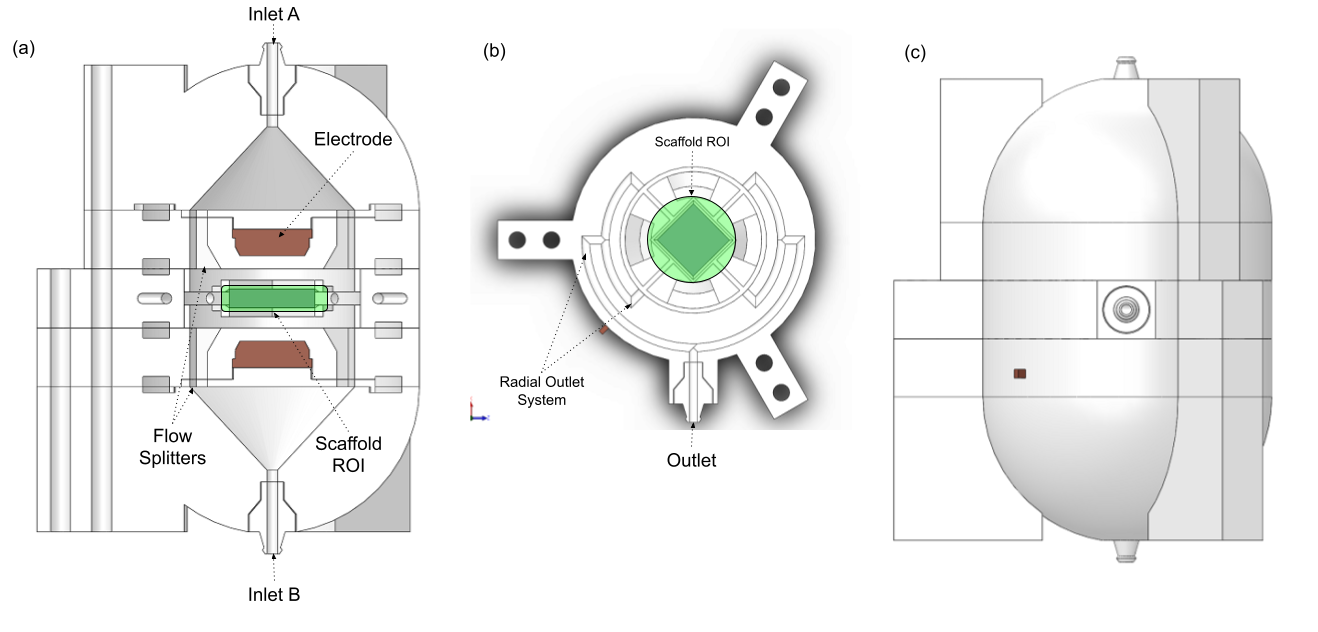
\includegraphics[scale=0.35]{./figures/Figure_3d1}}
\caption{Novel bioreactor design: (\textbf{a}) Vertical cut view of the bioreactor design with parallel electrodes setup, the upper and bottom inlets, and the inlet flow splitters can be observed. (\textbf{b}) Horizontal cut view of the bioreactor design, where the radial outlet system can be observed. The green regions represent the \ac{ROI} where the scaffold and/or cell culture will be placed. This region was represented by a cylinder with a height of 4 \si{\milli\meter} and a diameter of 10 \si{\milli\meter}. (\textbf{c}) Bioreactor \ac{CAD} design assembled in frontal view, the outlet hose joiner is visible in the middle.}
\label{figReactorA}
\end{figure}   


\subsection{Modelling osteogenic promoting perfusion flow}

\ac{FEM} modelling was performed using the \ac{CFD} module from COMSOL Multiphysics software (version 5.2a, Stockholm, Sweden). A stationary study was performed with the \textit{Laminar Flow (spf)} physics interface, solving the equations for a single-phase incompressible fluid in the laminar flow regime, i.e. the Navier-Stokes equations for conservation of momentum and the continuity equation for conservation of mass (equations \ref{NS1}, \ref{NS2}, \ref{NS3}). 

\begin{equation}
\label{NS1}
\nabla \cdot u = 0
\end{equation}

\begin{equation}
\label{NS2}
\rho \frac{\partial u}{\partial t} + \rho u \cdot \nabla (u) = -\nabla p + \nabla \cdot (\mu (\nabla u + \nabla u^T)) + F
\end{equation}

\begin{equation}
\label{NS3}
\rho C_p \frac{\partial T}{\partial t} + \rho C_p u \cdot \nabla T = \nabla \cdot (k \nabla T) + Q
\end{equation}

\noindent were $u$ is the velocity field, $p$ represents the pressure, and $T$ the temperature of the fluid in the modeled domain. $F$ is the Navier-Stokes equation term that represents the external forces applied to the fluid. $\rho$ is the fluid kinematic viscosity, $k$ is the thermal conductivity of the fluid, $C_p$ is the specific heat, and $Q$ represents dissipation. Navier-Stokes equations follow the principle of conservation of the energy, momentum, and mass of a fluid flow. 

Our goal was to find which input stimulation fluid velocity originated proper osteogenic \ac{WSS} values. Osteogenic flow stimulation conditions were reported, for example, in experimental studies conducted by Zhao \textit{et al.} \cite{Zhao2018-ci}. Zhao \textit{et al.} work found that the optimal flow rates, under which the highest fraction of scaffold surface area is subjected to a wall shear stress that induces mineralization, are strongly dependent on the scaffold geometries. Nevertheless, the variation range of such optimal flow rates was found to be within 0.5 to 5 \si{\milli\liter\per\minute} (or fluid velocity: 0.166--1.66 \si{\milli\meter\per\second}). Those ranges were obtained considering different scaffold geometries and predictions from a mechano-regulation theory, where extracellular matrix mineralization would be stimulated with \ac{WSS} values previously reported as being osteogenic \cite{Zhao2018-ci}.

\begin{figure}
\makebox[\textwidth][c]{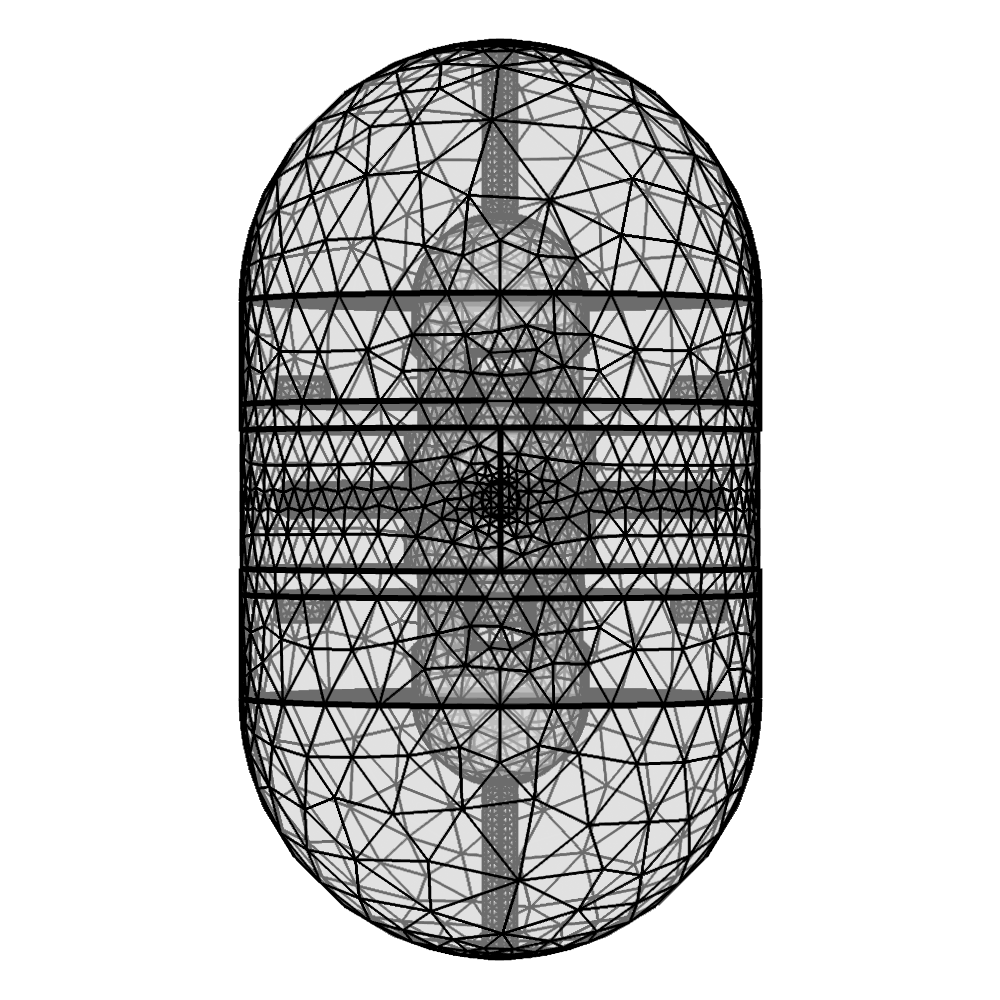
\includegraphics[scale=0.6]{./figures/Figure_3d2}}
\caption{Bioreactor geometry volume mesh created using COMSOL Multiphysics, with 1.9 $\times$ 10$^{6}$ elements and an average element quality of 0.65. External connector parts were excluded from \ac{FEM} analysis.}
\label{figMesh}
\end{figure}   

The \ac{CAD} model of the bioreactor was imported into COMSOL, where a physics-controlled mesh was generated with \num{1.9d6} tetrahedral volume elements and an average element quality of 0.65, as shown in Figure \ref{figMesh}. The final geometry comprised two distinct domains: one fluidic domain, made from culture medium material, and one construction domain, consisting of \acs{PETG} material. The temperature for this simulation was set at 37 \si{\degreeCelsius}. Regarding the COMSOL laminar flow study, the fluid domain representing the culture medium was assumed to be a homogeneous and incompressible Newtonian fluid with a volume density of 993.3 \si{\kilo\gram\per\cubic\meter} and dynamic viscosity of \num{6.9d-4} \si{\pascal}$\cdot$\si{\second}. Considering that the \acs{ROI} diameter is 0.010 \si{\meter}, and the fluid velocity in the same region was established at 0.0016 \si{\meter\per\second} \cite{Zhao2018-ci}, the calculated Reynolds number was 18.51, which is less than the threshold for turbulent flow (2300) \cite{Chen2019-cl}, so a single-phase laminar flow regime was also considered. The \ac{GMRES} solver was selected with adaptive meshing for local solution improvement. Boundary conditions were set for all bioreactor's walls with a no-slip condition. This boundary condition is valid for low-viscosity fluids at all fluid-solid boundaries, meaning that the fluid velocity is considered zero at the surface interface, starting to increase in the flux region right above the no-slip layer. The outlet was set at a reference constant pressure of one atmosphere (101.325 \si{\pascal}), while the two inlets were set at the same value for inflow velocity, assuming the velocity vector field as normal to the inlet surface. Multiple inlet conditions were introduced into \ac{FEM} until the results predicted the desired fluid velocity/shear stress values at the \ac{ROI} that adequately translate osteogenic conditions in the scaffold cell culture region.


\subsection{Adapting perfusion bioreactor design to limiting hardware}

The previously presented multimodal perfusion bioreactor design was expanded to support a single large bone-defect scaffold (with the same size as the non-healing fracture). To accomplish this, the \ac{ROI} was increased to a cylindrical region (diameter=30 mm, height=5 mm) placed concentrically at the center of the bioreactor, equally distant from both splitter components (Figure \ref{fig3d3}). This bioreactor \ac{CAD} was also adapted to operate with velocity-limiting peristaltic pump hardware, here represented by a peristaltic pump equipment model from Reglo Digital (Ismatec, Germany), with output flow rate dependent on the tubing used. Constraints imposed by the standard fuse deposition modelling (\acs{FDM}) 3D printing process determined that the internal tube diameter of bioreactor inlet tube fittings has to be superior to 2.40 \si{\milli\meter} (1.80 \si{\milli\meter} - channel, plus 2x0.30 \si{\milli\meter} - walls). According to Ismatec, one manufacturer of peristaltic tubing, the most approximate tubing available that meets these necessary conditions has 2.54 \si{\milli\meter} of internal diameter, which will provide a maximum peristaltic pump flux of 8.3 \si{\milli\liter\per\minute} for the equipment considered, originating a bioreactor inlet velocity of 0.0542 \si{\meter\per\second} (applied equally to both inlets). The optimization of the culture medium flow was obtained by geometrically adjusting and redesigning two components of the bioreactor: the inlet cap component, where the culture medium flow enters the bioreactor and is redirected to multiple feeding channels, and the flow splitter component, where the flow is divided and oriented to the cell culture \ac{ROI}.

\begin{figure}
\makebox[\textwidth][c]{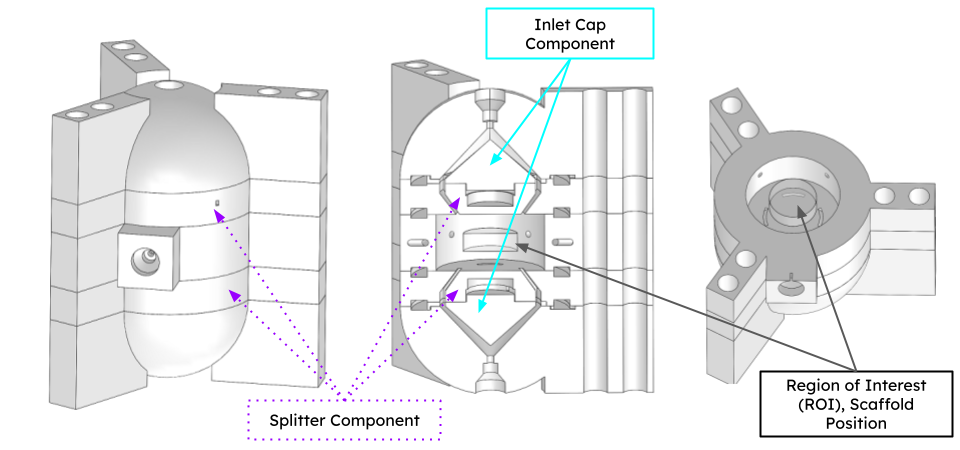
\includegraphics[scale=0.5]{./figures/Figure_3d3}}
\caption{Optimized bioreactor design. (A) Full view of the bioreactor exterior; (B) Vertical slice illustrating the bioreactor
interior; (C) Horizontal slice showing the \ac{ROI}. The blue and purple arrows identify components under optimization, while
the \ac{ROI} is identified by the black arrows.}
\label{fig3d3}
\end{figure} 




\section{Results}


\subsection{Modelling osteogenic promoting perfusion flow}

Several inlet velocities were tested to find a combination of inlet and outlet flow conditions to originate a flow range in the \ac{ROI} similar to the one reported in Zhao \textit{et al.} \cite{Zhao2018-ci}. \ac{FEM} results conduced to an inlet velocity of 0.003 \si{\meter\per\second} at each bioreactor inlet, combined with an outlet constant pressure value of one atmosphere. The laminar flow study predicted an average velocity of \num{1.14d-4} \si{\meter\per\second} and an average pressure of 0.6 \si{\pascal}, generating a flow of 2.58 \si{\milli\liter\per\minute} in the \ac{ROI}, which is within the considered range of 0.5 to 5 \si{\milli\liter\per\minute} used for obtaining maximum mineralization in bone tissue engineering, according to the work performed by Zhao \textit{et al.} \cite{Zhao2018-ci}. Velocity and pressure distributions predicted inside the bioreactor model are presented in Figure \ref{figResultsA}.

\begin{figure}
\makebox[\textwidth][c]{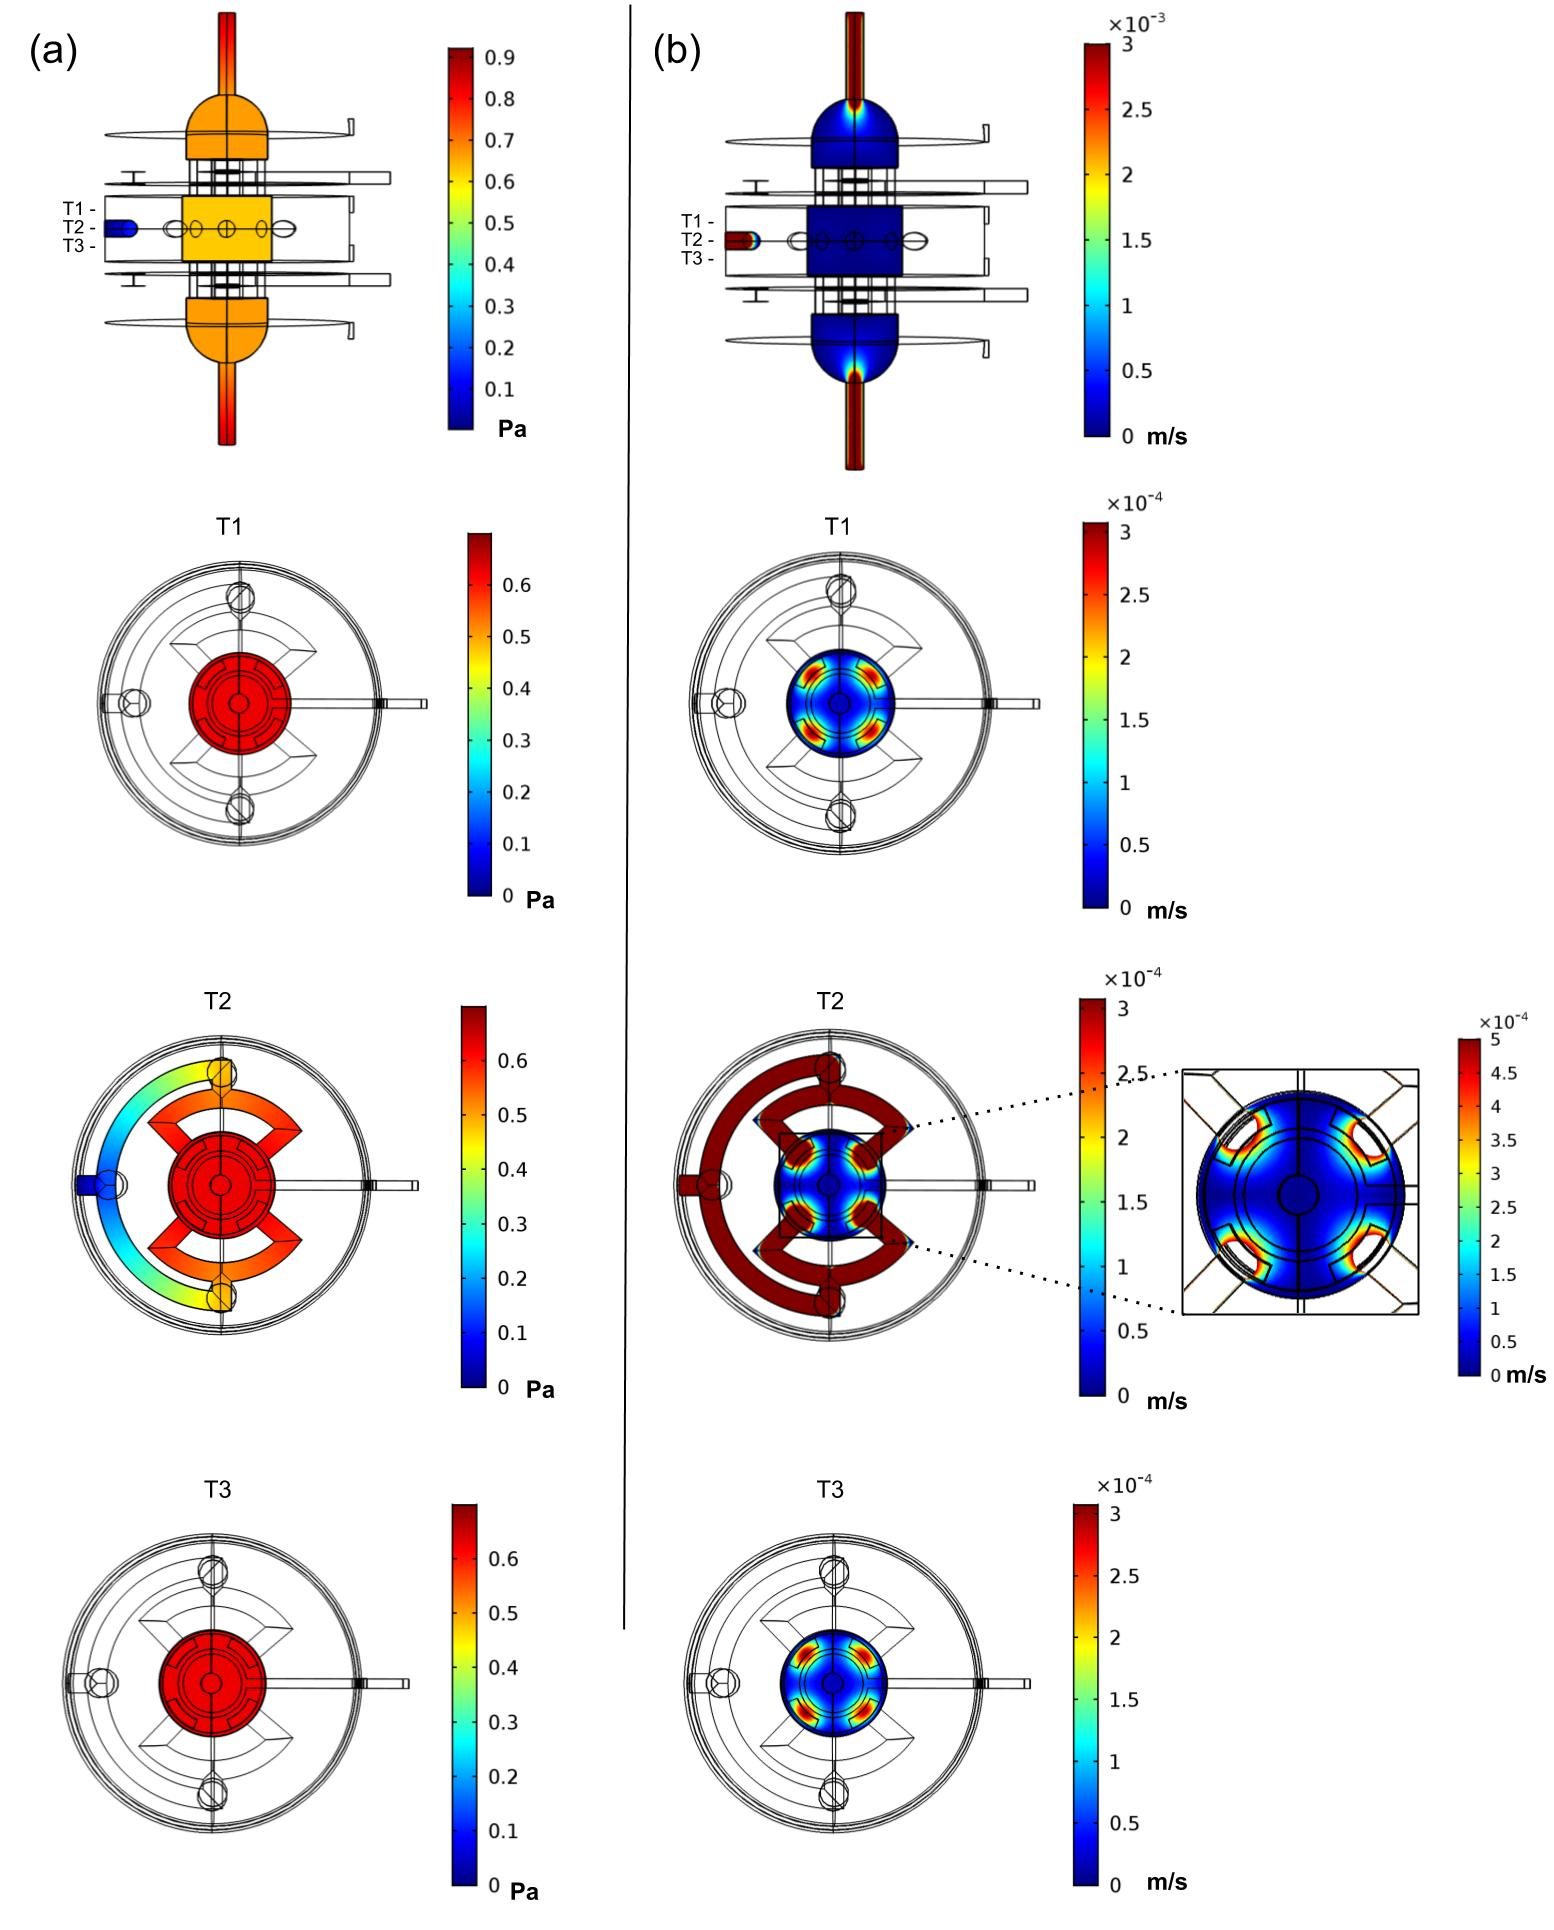
\includegraphics[scale=0.22]{./figures/Figure_3d4}}
\caption{\ac{FEM} analysis of the proposed bioreactor design for a laminar perfusion flow with lateral (upper row) and top slice views. The three top views represent the \ac{ROI} upper slice (T1), the \ac{ROI} middle plane slice (T2), and the ROI bottom slice (T3).  (\textbf{a}) Pressure distribution predicted considering applied inlet velocity of 0.003 \si{\meter\per\second} and outlet pressure of one atmosphere. (\textbf{b}) Fluid velocity distribution predicted for the same inlet/outlet conditions. The velocity distribution at the \ac{ROI} middle plane slice is presented in more detail in a top-view inset at the right of the slice plane.}
\label{figResultsA}
\end{figure}


\subsection{Adapting perfusion bioreactor design to limiting hardware}

\textit{Inlet cap component optimization.} The main goal was to reduce the flow velocity loss at the output of this component. For this purpose, three design hypotheses were tested (Figure \ref{figInlet}): (E) initial design starting point; (F) size reduction applied to all output channels; (G) pyramidal fill added to design hypothesis F. This design hypothesis were created considering that progressively directing the inlet flow to the output channels through a shorter path would lead to higher velocities. \ac{FEM} analyses were run independently for the three inlet component hypotheses. Hypothesis G was predicted to be the most suitable design for the established goal, since it increased the outflow average velocity to 0.0021 \si{\meter\per\second} per channel (26 times less than the bioreactor inlet velocity), in comparison to the design hypothesis E, where the outflow average velocity was predicted to be 50 times less than the bioreactor inlet velocity (Figure \ref{figInletResult}). Compared with design hypothesis F, design G results in the same outflow average velocity, but it requires less fluid to operate, which is an advantage in \ac{TE} applications due to the costs of the cell culture medium. Therefore, design G was chosen because it improves outflow average velocity and reduces liquid volume requirement.

\begin{figure}
\makebox[\textwidth][c]{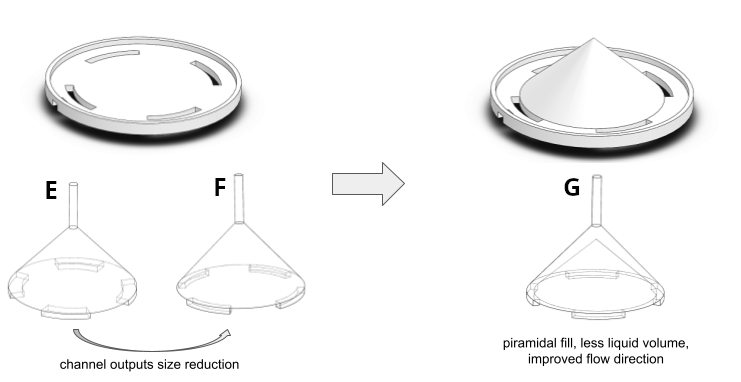
\includegraphics[scale=0.55]{./figures/Figure_3d5}}
\caption{Inlet component optimization: illustration of design hypotheses E, F, and G.}
\label{figInlet}
\end{figure}

\begin{figure}
\makebox[\textwidth][c]{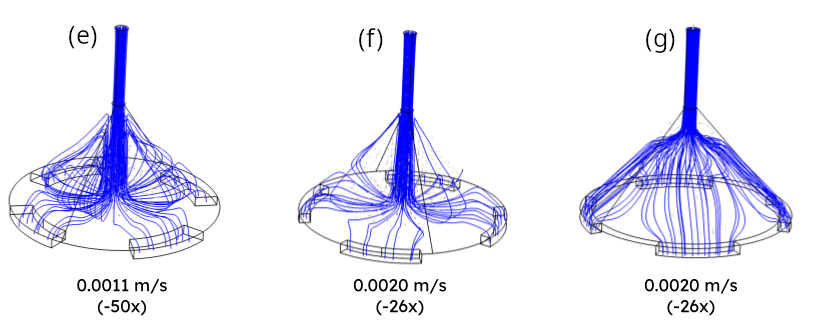
\includegraphics[scale=0.5]{./figures/Figure_3d6}}
\caption{Inlet component optimization: streamlines representing the fluid flow for each design hypothesis. The estimated
average outflow velocity and the number of times above the inlet velocity are indicated below in parentheses.}
\label{figInletResult}
\end{figure} 


\textit{Splitter component optimization.} For this component and augmented bioreactor dimensions, the main goal was to obtain the generated fluid flow-induced \ac{WSS} in the \ac{ROI} within the range of 0.11 - 60 \si{\milli\pascal}, as determined previously by Zhao \textit{et al.}, since this \ac{WSS} range was observed to effectively promote osteogenic differentiation and improve bone matrix secretion \cite{Zhao2018-ci}. First, the inlet component design shown in Figure \ref{figInlet}c was assumed as part of the bioreactor. Then, the entire liquid volume was filled, and the cylindrical \ac{ROI} was placed in the middle of the bioreactor. Four design hypotheses were tested, each assuming design variations in channel size and configuration that will originate different fluid flow velocities and directions. The tip of the channel size was progressively decreased, and its direction is progressively pointed towards the \ac{ROI} (Figure \ref{figSplitter}). Channel sizes hypothesis: A - 3.86 \si{\milli\meter}; B - 2.00 \si{\milli\meter}; C - 1.50 \si{\milli\meter}; D - 1.00 \si{\milli\meter}. For Newtonian fluids, shear stress $(\tau_s)$ is related to the shear rate $(\tau_r)$, calculated with COMSOL, by using the kinematic viscosity $(\mu)$ with the following equation \ref{TAU}.

\begin{equation}
\label{TAU}
\tau_r = \tau_s/\mu
\end{equation}

Using this equation \ref{TAU}, the shear rate values should lie in the range of 0.15 - 86 \si{\per\second}, corresponding to a \ac{WSS} range of 0.11 - 60 \si{\milli\pascal} at the \ac{ROI} as pointed by Zhao \textit{et al.} \cite{Zhao2018-ci}. Design hypothesis D was predicted to have the most considerable average shear rate at the \ac{ROI} within the range determined above, with a mean value of 0.30 \si{\per\second} (max:0.71 \si{\per\second}, min:0.046 \si{\per\second}), thus it was considered to be the best splitter component to achieve the proposed goals for mechanical stimulation inside optimal osteoinductive ranges.

\begin{figure}
\makebox[\textwidth][c]{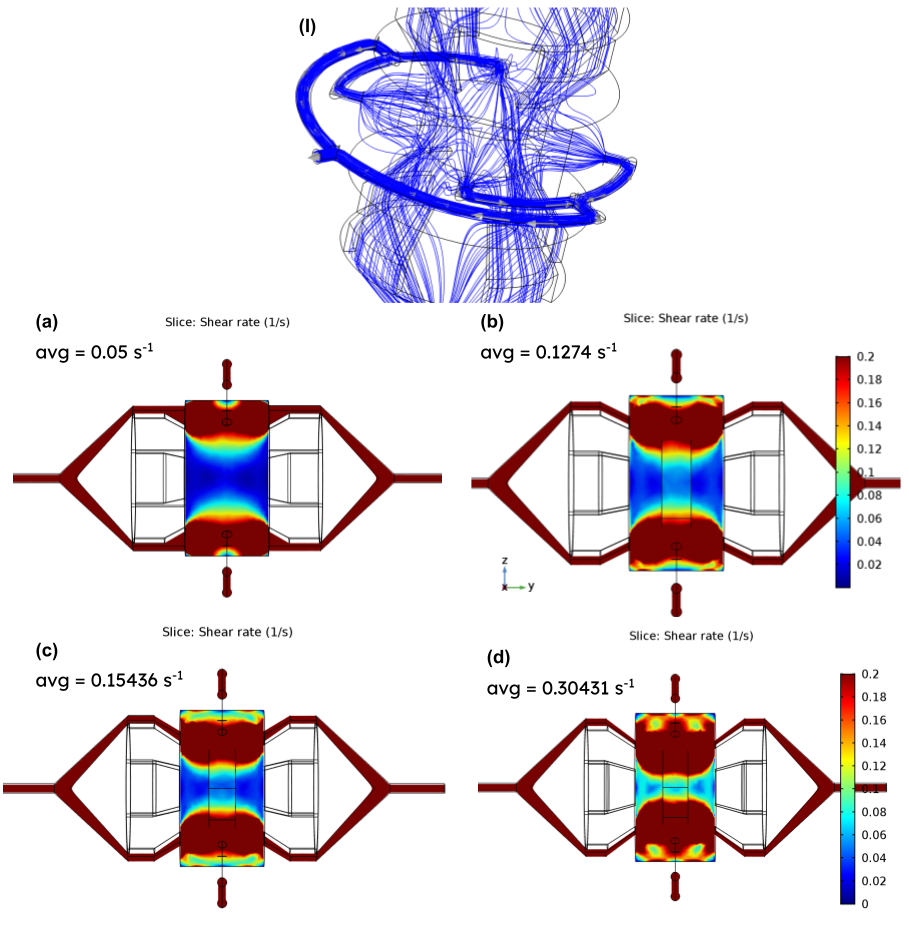
\includegraphics[scale=0.45]{./figures/Figure_3d7}}
\caption{(i) Shows the \ac{CFD} streamline plot for the center of the bioreactor, including a perspective over the outlet radial channels. Splitter component optimization: computer fluid dynamics results for fluid shear rate (1/s). The predicted shear rate average (avg) at the \ac{ROI} was calculated for each design hypothesis and is indicated below each figure index letter. Each channel end size tested hypothesis: (a) 3.86 \si{\milli\meter}; (b) 2.00 \si{\milli\meter}; ((c) 1.50 \si{\milli\meter}; (d) 1.00 \si{\milli\meter}.}
\label{figSplitter}
\end{figure} 




\section{Discussion}
This work demonstrated that applying a well-established \ac{CFD} numerical model is critical to predict and design the flow outcomes of a perfusion bioreactor. \ac{CFD} equations can be applied to predict fluid velocity, shear stress, and pressure stimulation conditions at the cell culture region and at other regions of the developed perfusion bioreactor design. These \ac{CFD} models can help find the input conditions needed to obtain or replicate a determined microenvironment in a custom design, like in the bioreactor proposed. Additionally, to adapt a protocol for a particular design, \ac{CFD} numerical models can be interactively used to shape and redesign parts or expand designs, generate specific mechanical stimulation hypotheses, or accommodate existing laboratory equipment that may constrain perfusion.  

Although empty chamber \ac{CFD} model predictions are adequate to compare different perfusion setups, introducing a cell culture scaffold will affect how the fluid flows. Thus, \ac{FEM} studies should consider the scaffold geometry to find the appropriate inlet/outlet conditions for each specific scaffold, a subsequently conducted study that its described in Chapter 6. The mechanical stimulation systems that act through fluidic interactions need to take into account the geometry of the scaffold once it creates different stimulation regions by shaping the microfluidic dynamics, as observed by Porter \textit{et al.} \cite{Porter2005-fd}, and predicted numerically by others \cite{Seddiqi2020-ti, Saatchi2020-bg}. In an original approach, Li \textit{et al.} \cite{Li2009-wu} manipulated fluid flow velocity and viscosity (by using dextran concentration) to be able to treat fluid flow-induced shear stress and mass transport as independent variables. They observed that, for $\beta$-tricalcium phosphate scaffolds seeded with \ac{MSCs}, that increasing flow-induced shear stress accelerated osteogenic differentiation and improved mineralization, while increased mass transport inhibited \ac{ECM} mineralization. The \ac{CFD} models proposed in this chapter were recently applied by Capuana \textit{et al.} \cite{Capuana2023-ik} to an airlift perfusion bioreactor in two stages: first, considering the entire bioreactor apparatus with a scaffold support multigrid; second, considering a micro-computed tomography of a region of a \acs{PLLA} scaffold produced by thermally induced phase separation. They confirm their two-step numerical predictions as essential to understand the turbulent characteristics generated by their developed bioreactor. Our bioreactor design concepts are conceived to create laminar flow conditions, reducing the numerical model's complexity and thus reinforcing the confidence in the numerical predictions. Posteriorly, adding scaffold structures, performing the cell seeding process, and even cell proliferation, growth, and external cellular matrix secretion will impact how fluid flows and the resultant shear stress is delivered to cells. This phenomenon needs to be further addressed.  

To fully take advantage of \ac{CFD} models' potential, these must be validated for each bioreactor/scaffold design combination, considering the limitations imposed by existing laboratory equipment. Validated models could then be applied to control, update, and optimize mechanical stimulation conditions in real-time \cite{Post2022-pr}. Also, refining mechanical stimulation protocols and their delivery may improve the understanding of cellular mechanotransduction responses.



\section{Summary}
This chapter proposes a novel design of a perfusion bioreactor for \ac{BTE} \textit{in vitro} applications. This design allows the application of fluid flow-induced shear stress aiming at more significant outcomes in cell differentiation, migration, and proliferation with bone cell lines. It also underlines the importance of combining \ac{3D} \ac{CAD} design and \ac{CFD} numerical modelling simulations to find the optimal input that generates the desired stimulation ranges, informed by previous experimental studies, and to optimize outcomes for \ac{TE} purposes. A data-driven design approach based on numerical predictions will be essential to create and optimize experimental conditions to understand the underlying biophysical effects of mechanical stimuli in cell cultures. It can be a powerful tool for standardizing stimulation protocols considering different bioreactor designs, diverse lab equipment, and specific BTE outcomes. The CFD framework applied here will be further explored in Chapter 6, where all individual numerical models were combined into a multimodal stimulation bioreactor design strategy.  


%\newpage
%\bibliography{library_c3b} 
%\bibliographystyle{plain}
%\end{document}
%\documentclass[11pt]{report}
%\usepackage{siunitx}
%\usepackage{graphicx}
%\usepackage{multirow}
%\usepackage[table,xcdraw]{xcolor}
%
%\begin{document}
%\setcounter{chapter}{3}
%\tableofcontents



\newpage
\chapter{Numerical modelling of direct-coupled stimulation}
This chapter contains the results of the numerical modelling approaches applied for direct-coupled (DCoupled) electric field setups. This chapter's contents were collected from the following work:
\begin{itemize}
\item \small \textit{''Direct coupled electrical stimulation towards improved osteogenic differentiation of human mesenchymal stem/stromal cells: a comparative study of different protocols.'', João C. Silva and João Meneses, Fábio F.F. Garrudo, Sofia R. Fernandes, Nuno Alves, Frederico Castelo Ferreira, and Paula Pascoal-Faria, work under review at Nature Scientific Reports.} 
\end{itemize}

This chapter's required cell culture procedures were made in collaboration with the SCERG - Stem Cell Engineering Research Group from iBB/IST - Instituto Superior Técnico, Portugal. Results from this work also gave rise to updated versions of the DCoupled electric field stimulation setup presented here and enhanced stimulation protocols applied to bone marrow-derived mesenchymal stem/stromal cells. This subsequent study will be available at:
\begin{itemize}
\item \small \textit{''Synergy between 3D-extruded electroconductive scaffolds and electrical stimulation in enhancing bone regeneration.'', João C. Silva, Pedro Marcelino, João Meneses, Frederico Barbosa, Carla S. Moura,e Ana C. Marques, Joaquim M. S. Cabral, Paula Pascoal-Faria, Nuno Alves, Jorge Morgado, Frederico C. Ferreira, Fábio F. F. Garrudo, work under submission.}
\end{itemize}  





\newpage
\section{Introduction}
The application of a \ac{DCoupled} constant current stimulation protocol constitutes a simple and straightforward approach shown to promote multiple cellular responses, ranging from cell migration to proliferation and differentiation \cite{Guillot-Ferriols2022-wn, Song2007-qr}. Bioelectric cues function alongside chemical gradients, transcriptional networks, and haptic/tensile cues as part of the morphogenetic field that orchestrates individual cell responses \cite{Tseng2013-yx, Da_Silva2020-su, Guillot-Ferriols2022-wn}. Electrical stimulation cues are considered a valuable tool to guide cells into desirable \ac{TE} outcomes and ultimately unlock the potential of tissue engineering approaches for therapeutic applications \cite{Da_Silva2020-su}.

Electric stimulation has been used clinically for over four decades to promote bone healing, mainly as an adjunct to standard fracture care \cite{Bassett1974-rb}. Several \textit{in vitro} and \textit{in vivo} studies have been conducted by applying DCoupled stimulation to undifferentiated stem cells and differentiated osteoblast cells through the use of different setups, electrode or substrate materials and a variety of waveforms \cite{Guillot-Ferriols2022-wn, Ryan2021-tq, Thrivikraman2018-su}. Accordingly, a study performed by Wang \textit{et al.} demonstrated that a current-base DCoupled protocol (4 \si{\micro\ampere}, 3 \si{\hour} per day for 14 days) enhanced significantly the proliferation and osteogenic differentiation of MC3T3-E1 preosteoblastic cells \cite{Wang2021-tm}. Moreover, Srirussamee and colleagues reported that a daily direct electrical stimulation of 2.2 \si{\volt} for 1 \si{\hour} during a total period of 7 days promoted the \textit{in vitro} osteogenesis of human bone marrow-derived \ac{MSCs}, as evidenced by the significant upregulation of bone-specific marker gene SPP1 \cite{Srirussamee2021-cj}. Mesenchymal stem/stromal cells are a promising cell source for bone repair and have been playing a significant role in \ac{BTE} strategies due to their ability to differentiate towards osteogenic lineage, accumulating other selective advantages like their high availability (since they reside in many organs and tissues of the body), their high in vitro proliferation capacity, low immunogenicity and advantageous immunomodulatory/trophic features \cite{Arthur2020-bs, Silva2020-sw}. Bone marrow-derived MSCs (BMSCs) are considered “gold standard” sources for cell-based therapies, and due to their nature as bone residents, they have been widely used in BTE strategies \cite{Rossi2023-od, Shang2021-ty, Silva2020-dc}. 

The mechanisms behind electrically-driven cellular processes rely on the modulation of membrane potentials by endo or exogenous \ac{EFs} \cite{Thrivikraman2018-su}. The scarcity of predictive models to guide and estimate the experimental \acs{EFs} delivered upon \ac{DCoupled} stimulations has led researchers to rely on the applied input electric potential or on the electric potential drop between the electrodes as a stimulation magnitude comparator between different studies. However, these values do not translate the \acs{EF} effectively delivered to cells, since they do not take into account the critical dielectric properties of the materials involved, the geometry of the electrodes and stimulation chamber, or the complex electrode/electrolyte interface effects \cite{Guette-Marquet2021-rp}. An exception was made by a few studies modelling DC stimulation. Srirussamee \textit{et al.} \cite{Srirussamee2021-cj} designed an electrochemical-based \ac{FEM} model considering a secondary current distribution ruled by Ohm’s law that also accounts for charge transfer reactions, following the Butler-Volmer equation. Two other studies were conducted by Zimmermann \textit{et al.} \cite{Zimmermann2021-fx, Zimmermann2023-gm}. One tackled a \ac{DCoupled} \ac{EF} stimulation \ac{FEM} model that solves Laplace’s equation and accounts for electrode-electrolyte interface interactions, by adjusting the solution to experimental current measurements, and by previously calibrating model parameters with results from electrochemical characterization \cite{Zimmermann2021-fx}. Another work from the same authors presents experimental and numerical methods to calculate the delivered \ac{EF} and current density, including procedures with lumped-element and a \ac{FEM} model approach \cite{Zimmermann2023-gm}. Notably, the widespread implementation of digital models would be highly advantageous to improve current \ac{BTE} methods, since they will allow the optimization of stimulation protocols and the development of predictive platforms, while at the same time reducing experimental time and associated costs \cite{Moller2021-kr, Geris2018-tz}.

The work described in this chapter replicates the \ac{DCoupled} setup originally conceived by Mobini \textit{et al.} \cite{Mobini2016-jh} and further applied in many subsequent studies \cite{Mobini2017-wp, Mobini2017-zr, Leppik2018-bw, Moon2023-rm}. Distinctively from \cite{Mobini2016-jh}, we created a 6-well plate custom lid with L-shaped electrodes made of medical-grade stainless steel wire instead of pure platinum. This work explored the influence of different electric stimulation parameters on \acs{MSCs} osteogenesis. Each applied protocol was guided by an electrical characterization of the \ac{DCoupled} resultant waveform, to individually understand the biological impact of different parts of a typical stimulation waveform. A finite-element model of one of the 6 wells was designed and used to simulate and predict the \ac{EFs} induced by the DCoupled protocols applied. With the results from the developed \ac{DCoupled} setup characterization and correspondent setup digital model, this work also hypothesizes if \ac{DCoupled} electric stimulation performed below the water electrolysis potential remains capable of producing similar osteoinductive effects in \ac{MSCs} as previously reported at higher potentials \cite{Mobini2016-jh, Mobini2017-wp, Mobini2017-zr, Leppik2018-bw}. Also, we explore, with the same constant potential step, what are the differences in terms of osteoinductive effects when applying a very short stimulation exposure versus a more prolonged exposure typical of DCoupled stimulation literature \cite{Mobini2016-jh, Mobini2017-wp, Mobini2017-zr, Leppik2018-bw}. Additionally, the generated protocols allow us to better understand the differences when applying an intermittent step with two distinct frequencies versus a steady electric potential step. A constant current condition was also explored, allowing one of the electrodes to float its potential accordingly. This work contains one of the first studies to directly compare potential-controlled electric stimulation with current-controlled electric stimulation protocols to enhance the osteogenic differentiation of human \acs{MSCs}. All protocols were compared regarding their ability to promote bone marrow-derived \acs{MSCs} viability, proliferation, and osteogenic differentiation.


\section{Aims}
The work described in this chapter has the following main goals:
\begin{itemize}
\item Address the electrode/electrolyte relation in a \acs{BTE} typical \acs{DCoupled} setup;
\item Develop a numerical model to predict the \acs{EF} applied by a custom-developed \acs{DCoupled} setup;
\item Validate the developed model against the reported \acs{EF} from other researchers' \acs{DCoupled} setups;
\item Observe if \acs{DCoupled} electric stimulation, when performed below the water electrolysis potential, remains capable of producing similar osteoinductive effects, as previously reported for \acs{MSCs} subjected to higher potential protocols;
\item Explore differences in \acs{MSCs} effects when subjected to different stimulation protocols parameters: short \acs{DCoupled} stimulation exposure versus a longer exposure; intermittent step waveform with two distinct frequencies; steady electric potential step versus a constant current condition.  
\end{itemize}



\section{Methods}

\subsection{\acs{DCoupled} electrical stimulation system}
Electrical stimulation system custom lids (see Figure \ref{fig4d1}) for a 6-well plate (Falcon\textregistered, Corning, USA) polystyrene tissue culture-treated were designed and \ac{3D} printed in \acs{C8} material (3d4makers, Netherlands) \cite{Meneses2020-dx} by fuse deposition modelling technique (Creatbot F430, Henan Suwei Electronic Technology Co., China). The custom lid computer-aided design files are available for download at Figshare (https://doi.org/10.6084/m9.figshare.23629926.v1). Medical grade stainless steel wire 316LVM (Tegra Medical, Franklin, USA), with a 1 \si{\milli\meter} diameter, was manually bent into an L-shape (width 22 \si{\milli\meter}, height 18 \si{\milli\meter}) and used as electrodes, similarly to Mobini \textit{et al.} \cite{Mobini2016-jh}. Each L-shaped electrode was inserted at its respective hole at the top of the custom lid and glued by a drop of commercial silicone, remaining separated by a distance of 25 \si{\milli\meter} to the next electrode in the same well (Figure \ref{fig4d1} (a)-(c)). The described electrode pair per well constitutes the \ac{DCoupled} electric stimulation system.

Every row of three wells was connected to guarantee that the same electrical current and, correspondingly, the same \acs{EF} were applied across these three wells. Figure \ref{fig4d1}(d) shows the electrical connection schematic. Each row ($n=3$) was then subjected to an electric potential or electric current, with duration and characteristics according to the required stimulation protocol to be applied. The electric potential step application, constant or intermittent, was performed by a lab power source equipment (Tektronix, Berkshire, UK). The electric current application was performed by a custom current source electric circuit (Figure \ref{fig4d2}), composed of an operational amplifier (model TLV 2302), a PNP transistor (model PNP BC 556), and a 100-ohm resistor ($R$), wired according to Figure \ref{fig4d2}. This electric circuit requires a power source ($V_{cc}$) of 12 \si{\volt}, a ground reference, and a potential input ($V_i$) that allows the control and adjustment of the electric current output ($I_e$), following the expression: $I_e=(V_{cc}-V_i)/R$ (see Figure \ref{fig4d2}). The output of each potential or current source condition was measured and validated with a multimeter (ISO-TECH IDM 73, Ahaus, Germany) before its application. 

\begin{figure}
\makebox[\textwidth][c]{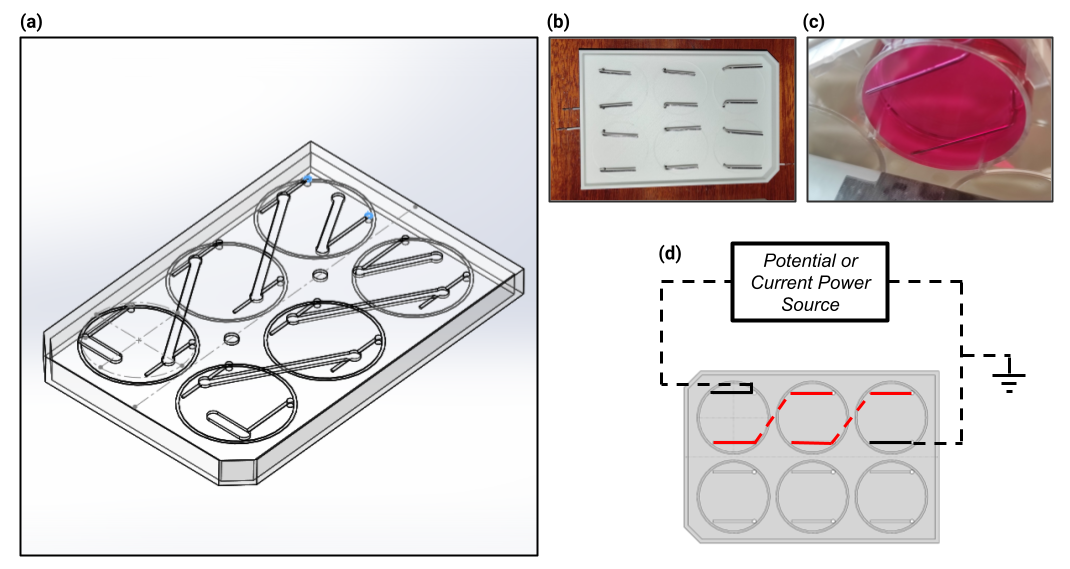
\includegraphics[scale=0.40]{./figures/Figure_4d1.png}}
\caption{\acs{DCoupled} electrical stimulation setup. (a) CAD of the developed custom lid; (b) Bottom view of the custom lid with the L-shape electrodes in medical grade stainless steel wire 316LVM; (c) Bottom view of a single well with electrodes, filled with culture media; (d) Diagram illustrating the electric connection in series of the three wells.}
\label{fig4d1}
\end{figure} 

\begin{figure}
\makebox[\textwidth][c]{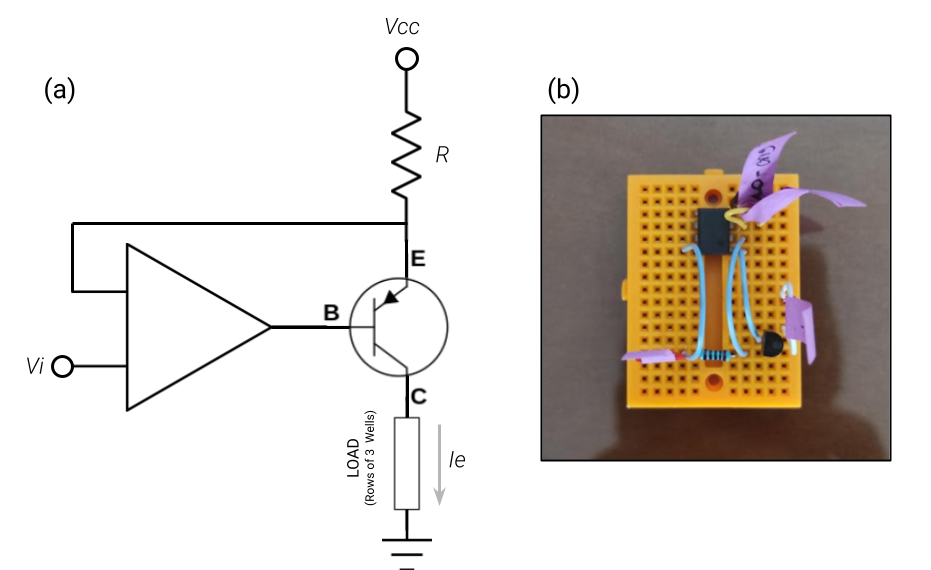
\includegraphics[scale=0.35]{./figures/Figure_4d2.png}}
\caption{Electric circuit of the custom current source developed for the \acs{DCoupled} setup. (a) Diagram of the electric circuit; (b) Image of the corresponding assembled breadboard with the required electronic components.}
\label{fig4d2}
\end{figure} 

\subsection{Determination of culture medium electrical conductivity}
Standard basal media (BM) is composed of Dulbecco’s modified eagle medium (DMEM, Gibco Thermofisher Scientific, Waltham, MA, USA) supplemented with 10\si{\percent} fetal bovine serum (FBS, MSC qualified, Gibco, Thermofisher Scientific) and 1\si{\percent} Antibiotic-antimycotic (Anti-Anti, Gibco, Thermofisher Scientific). Osteogenic culture media (OM) is composed of DMEM + 10\si{\percent} FBS(MSC) + 1\si{\percent} Anti-Anti supplemented with 10 \si{\milli\molar} beta-glycerolphosphate (Sigma-Aldrich, St. Louis, MO-IL, USA), 10  \si{\nano\molar} dexamethasone (Sigma-Aldrich) and 50 \si{\micro\gram\per\milli\liter} ascorbic acid (Sigma-Aldrich). Standard basal culture medium and osteogenic medium electrical conductivities were measured at room temperature (21 - 23 \si{\celsius}) and 37 \si{\celsius} using a multimeter (ISO-TECH IDM 73).
 
\subsection{\acs{DCoupled} electrical stimulation system response characterization}
The response of a single well from the developed \acs{DCoupled} system was studied to determine if the electrode/electrolyte interaction between the stainless steel wire 316LVM and the osteogenic culture medium or basal medium was driven by a faradaic or non-faradaic process. Following the procedure described in the work of Biesheuvel \textit{et al.} \cite{Biesheuvel2018-wu}, we applied an electric current step input to one of the electrodes and fixed the other as ground. The electric potential at the first electrode was probed with an oscilloscope (Keysight DSOX 1102A, Santa Rosa, USA), checking if the resulting curve is likewise the faradaic or non-faradaic typical waveform, as explained by Biesheuvel \textit{et al.} \cite{Biesheuvel2018-wu}. An electric potential step was also applied in the same single well, and the resulting potential waveform at the interface electrode/electrolyte was registered with the same oscilloscope. The response of a row of three wells in series to a potential step of 1.2 \si{\volt} was also acquired to check if the interpretation of a single well result could be expanded to a three-in-a-row configuration. A multimeter (KLEIN TOOLS MM600, Chicago, USA) was used to register the electric current passing these three wells in series to the ground electrode (last well of the row). With this test setup, by applying a range of input potentials (from 0 to 4 \si{\volt}, at increasing steps of 0.5 \si{\volt}), we obtained an I-V curve for the system electrode/electrolyte interactions. The I-V curve was then used to compare the stainless steel wire 316LVM response with previously reported results from different electrode materials. 

\subsection{\acs{EF} predictions from \ac{FEM}}
To predict the \acs{EF} delivered by the \ac{DCoupled} system to the cellular content, a \acs{FEM} analysis was conducted with the AC/DC module of COMSOL Multiphysics (version 5.2a, www.comsol.com, Stockholm, Sweden). The Electric Current (ec) physics interface was selected, considering a stationary study, solving for current conservation (equation \ref{SC1}) and Faraday's law (steady currents derived equation \ref{SC2}).

\begin{equation}
\label{SC1}
\nabla \cdot J = 0
\end{equation}

\begin{equation}
\label{SC2}
\nabla \times E = 0
\end{equation}

\noindent where $J$ is the current density vector and $E$ is the electric field. This equations are then combined to describe materials where the current density is proportional to the electric field, resulting in the constitutional equation known as Ohm's law. Which when solved using the electrostatic potential ($\phi$) and the electric conductivity ($\sigma$) becomes Laplace's fundamental equation for steady currents \ref{SC3}:

\begin{equation}
\label{SC3}
\nabla \cdot (\sigma \nabla \phi) = 0
\end{equation}

A \ac{3D} physics-controlled mesh was generated in COMSOL with the finer mesh option. The model is composed of three material domains, characterized by their electrical conductivity ($\sigma$) and relative permittivity ($\epsilon_r$), according to Figure \ref{fig4d3}: stainless steel 316LVM for electrodes ($\sigma$: \num{1d5} \si{\siemens\per\meter}, $\epsilon_r$: 1); osteogenic culture medium at 37 \si{\celsius} ($\sigma$: \num{1.725} \si{\siemens\per\meter} - determined experimentally as described above, $\epsilon_r$: 80.1 \cite{Visone2018-sa}); polystyrene petri dish ($\sigma$: \num{6.7d-14}  \si{\siemens\per\meter}, $\epsilon_r$: 2.5). An electric potential step of 1.2 \si{\volt} was applied to obtain the current values for the I-V curve (avoiding water electrolysis by staying below the 1.23 \si{\volt} limit \cite{Guette-Marquet2021-rp}). Using this curve, we obtained a peak electric current of 0.17 \si{\milli\ampere}, followed by a drop in current to 0.03 \si{\milli\ampere} (see results section), both measures obtained for the osteogenic medium at 37 \si{\celsius}. These electric current conditions were then added to the model as a floating potential boundary condition to one of the electrodes while setting the other to a ground boundary condition. The average \acs{EF} was calculated at a disk shape region of interest, placed at the center of the well and equidistant from both electrodes (Figure \ref{fig4d3}a, \ref{fig4d3}b, \ref{fig4d3}c). The solution of the model was computed using the conjugate gradients iterative solver.


\begin{figure}
\makebox[\textwidth][c]{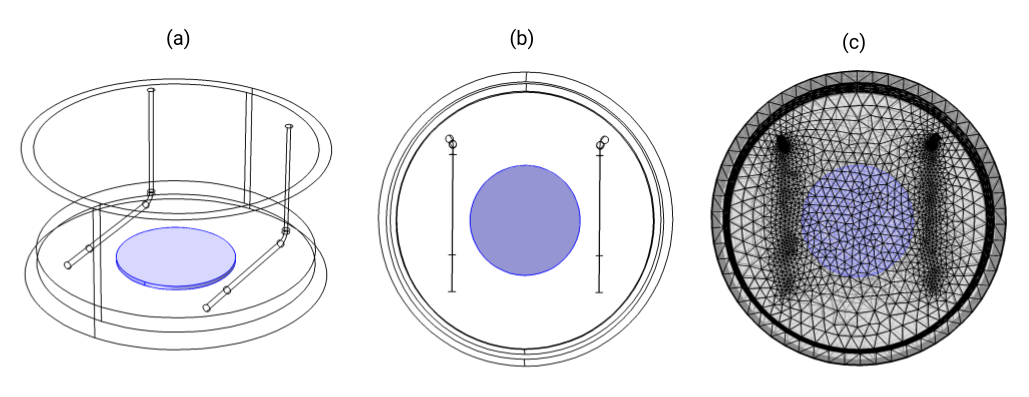
\includegraphics[scale=0.35]{./figures/Figure_4d3.png}}
\caption{\acs{FEM} model geometry of the \acs{DCoupled} setup. The central disk, in blue, represents the ROI under study. (a) Perspective view of the geometry; (b) Top view of the geometry; (c) Top view of the fine mesh.}
\label{fig4d3}
\end{figure}

Due to slight differences between the electrode's sizes, angles, and distances generated when hand-mounted into the custom lid, multiple electrode geometries were modeled inside a single culture well to study and understand the impact of minor geometrical variations on the delivered \acs{EF} prediction. Three geometry variation studies were performed: (1) distances between electrodes, 20 \si{\milli\meter} or 25 \si{\milli\meter}, keeping the same culture medium height and a constant electric current; (2) different culture medium heights, from 2 to 6 \si{\milli\meter}, comparing also between regular or shorter electrodes lengths, $\delta L \pm 5$ \si{\milli\meter}. For this study, we kept the electric current constant at \num{0.05} \si{\milli\ampere}; (3) regular position versus the worst-case tilt scenario, where one of the electrodes has an upper tilt of 5\si{\degree} and the other electrode has a bottom tilt of the same amplitude. Variation study (3) considered the same culture medium height of 5 \si{\milli\meter} and a constant electric current for the two test conditions.

\subsection{FEM model prediction for Mobini \textit{et al.} setup}
The FEM modelling approach described in the previous subsection was also applied to Mobini \textit{et al.} \cite{Mobini2016-jh} setup for \ac{FEM} model validation. Regarding geometric modelling, Mobini \textit{et al.} \cite{Mobini2016-jh} reported a cell culture dish diameter of \num{33.78} \si{\milli\meter} from a 6-well cell culture plate, with 128x85x22 \si{\milli\meter} (produced by TPP, Transadingen, Switzerland). Unfortunately, this well plate device is discontinued for the reported dimensions, but all the remaining models from the same supplier are produced in polystyrene material. The electrode wire has a diameter of 1 \si{\milli\meter} and was made from \num{99.99} \% pure platinum. This wire is reported to have a total length of 50 \si{\milli\meter} bent into an L-shape configuration, with 29-21 \si{\milli\meter} parts. Two electrodes per culture dish were separated by 25 \si{\milli\meter}. It is possible to estimate a wall thickness of 1 \si{\milli\meter} for the entire dish based on recent petri dish models. For the height, it is assumed the reported maximum plate height by the supplier is 22 \si{\milli\meter} (the actual dimension should have been shorter in older models). Also, regarding the reported distance between electrodes and in the absence of a detailed explanation, it was assumed from the wire center axis to the other wire center axis and not from the inner extremities. When trying to consider the inner extremities as the reference, the remaining reported dimensions have been shown to cause a superposition conflict with the reported dish wall position, resulting in an invalid CAD geometry. The distance of the electrodes to the dish bottom is not reported and was assumed to be \num{0.25} \si{\milli\meter}, remaining not in contact with the bottom. The culture medium volume used in each culture dish well was not reported. Still, for similar culture dish dimensions, the Thermo Fisher table about useful numbers in cell culture points \cite{Thermo} recommends a culture medium volume of 2 \si{\milli\liter}. Using this value in the geometrical model, we obtain a liquid volume height of \num{2.26} \si{\milli\meter}. 

Regarding finite element model considerations, the geometric model described in the previous step was imported into COMSOL. Culture dish, electrode and culture medium electrical properties were not measured but otherwise estimated or reported in the Mobini \textit{et al.} \cite{Mobini2016-jh} manuscript. So, to run COMSOL electric currents physics interface, electrical properties for the culture medium were obtained from \cite{Visone2018-sa}, $\sigma$: 1.5 \si{\siemens\per\meter}, $\epsilon_r$: 80.1. For polystyrene material electrical properties were retrieved from \cite{Plastic} with $\sigma$: \num{1.0d-18} \si{\siemens\per\meter} (reported $>$ \num{1.0d18} \si{\ohm\per\meter}), and $\epsilon_r$: 2.6 (interval 2.4 to 3.1). Platinum material $\sigma$ was assumed as \num{9.52d6} \si{\siemens\per\meter} (reported \num{1.05d-9} \si{\ohm\per\meter} \cite{Schuettler2007-zd}), and all metal's relative permittivity for lower frequencies is considered to be 1. The electric stimulus applied in this setup was a 2.2 \si{\volt} DC, as reported in the manuscript, generating an \acs{EF} of 100 \si{\milli\volt\per\milli\meter} (predicted) for this input electrical potential. To translate this to COMSOL, two boundary conditions were applied, one for ground in one electrode tip and another for the measured 0.07 \si{\milli\ampere} current \cite{Srirussamee2019-ai} that translates to a DC floating potential boundary condition on the opposite electrode tip. A normal-sized physics-controlled mesh was created, comprised of 19320 domain elements, 8080 boundary elements, and 721 edge elements. 

\subsection{Electrical stimulation protocol hypothesis}
With the information from the \acs{EF} numerical predictions and the DCoupled system electric response characterization, we created a group of electric stimulation conditions to test some hypotheses (see Figure \ref{fig_t4d1}). Two control cell culture conditions were created with no electrical stimulation protocol, one with basal media and the other with the osteogenic medium. The comparison between them allows us to infer the osteogenic medium effect alone. Then, we tested five cell culture conditions under different DCoupled electric stimulation protocols, all with the osteogenic medium. The potential or current step applied was the same as previously characterized, taking advantage of the characteristic DCoupled system response curve (see results section) when defining the stimulation protocol conditions. All-electric stimulation protocol conditions were applied every two days, stopping when we counted 14 days from the beginning of the experiment.

\begin{figure}
\makebox[\textwidth][c]{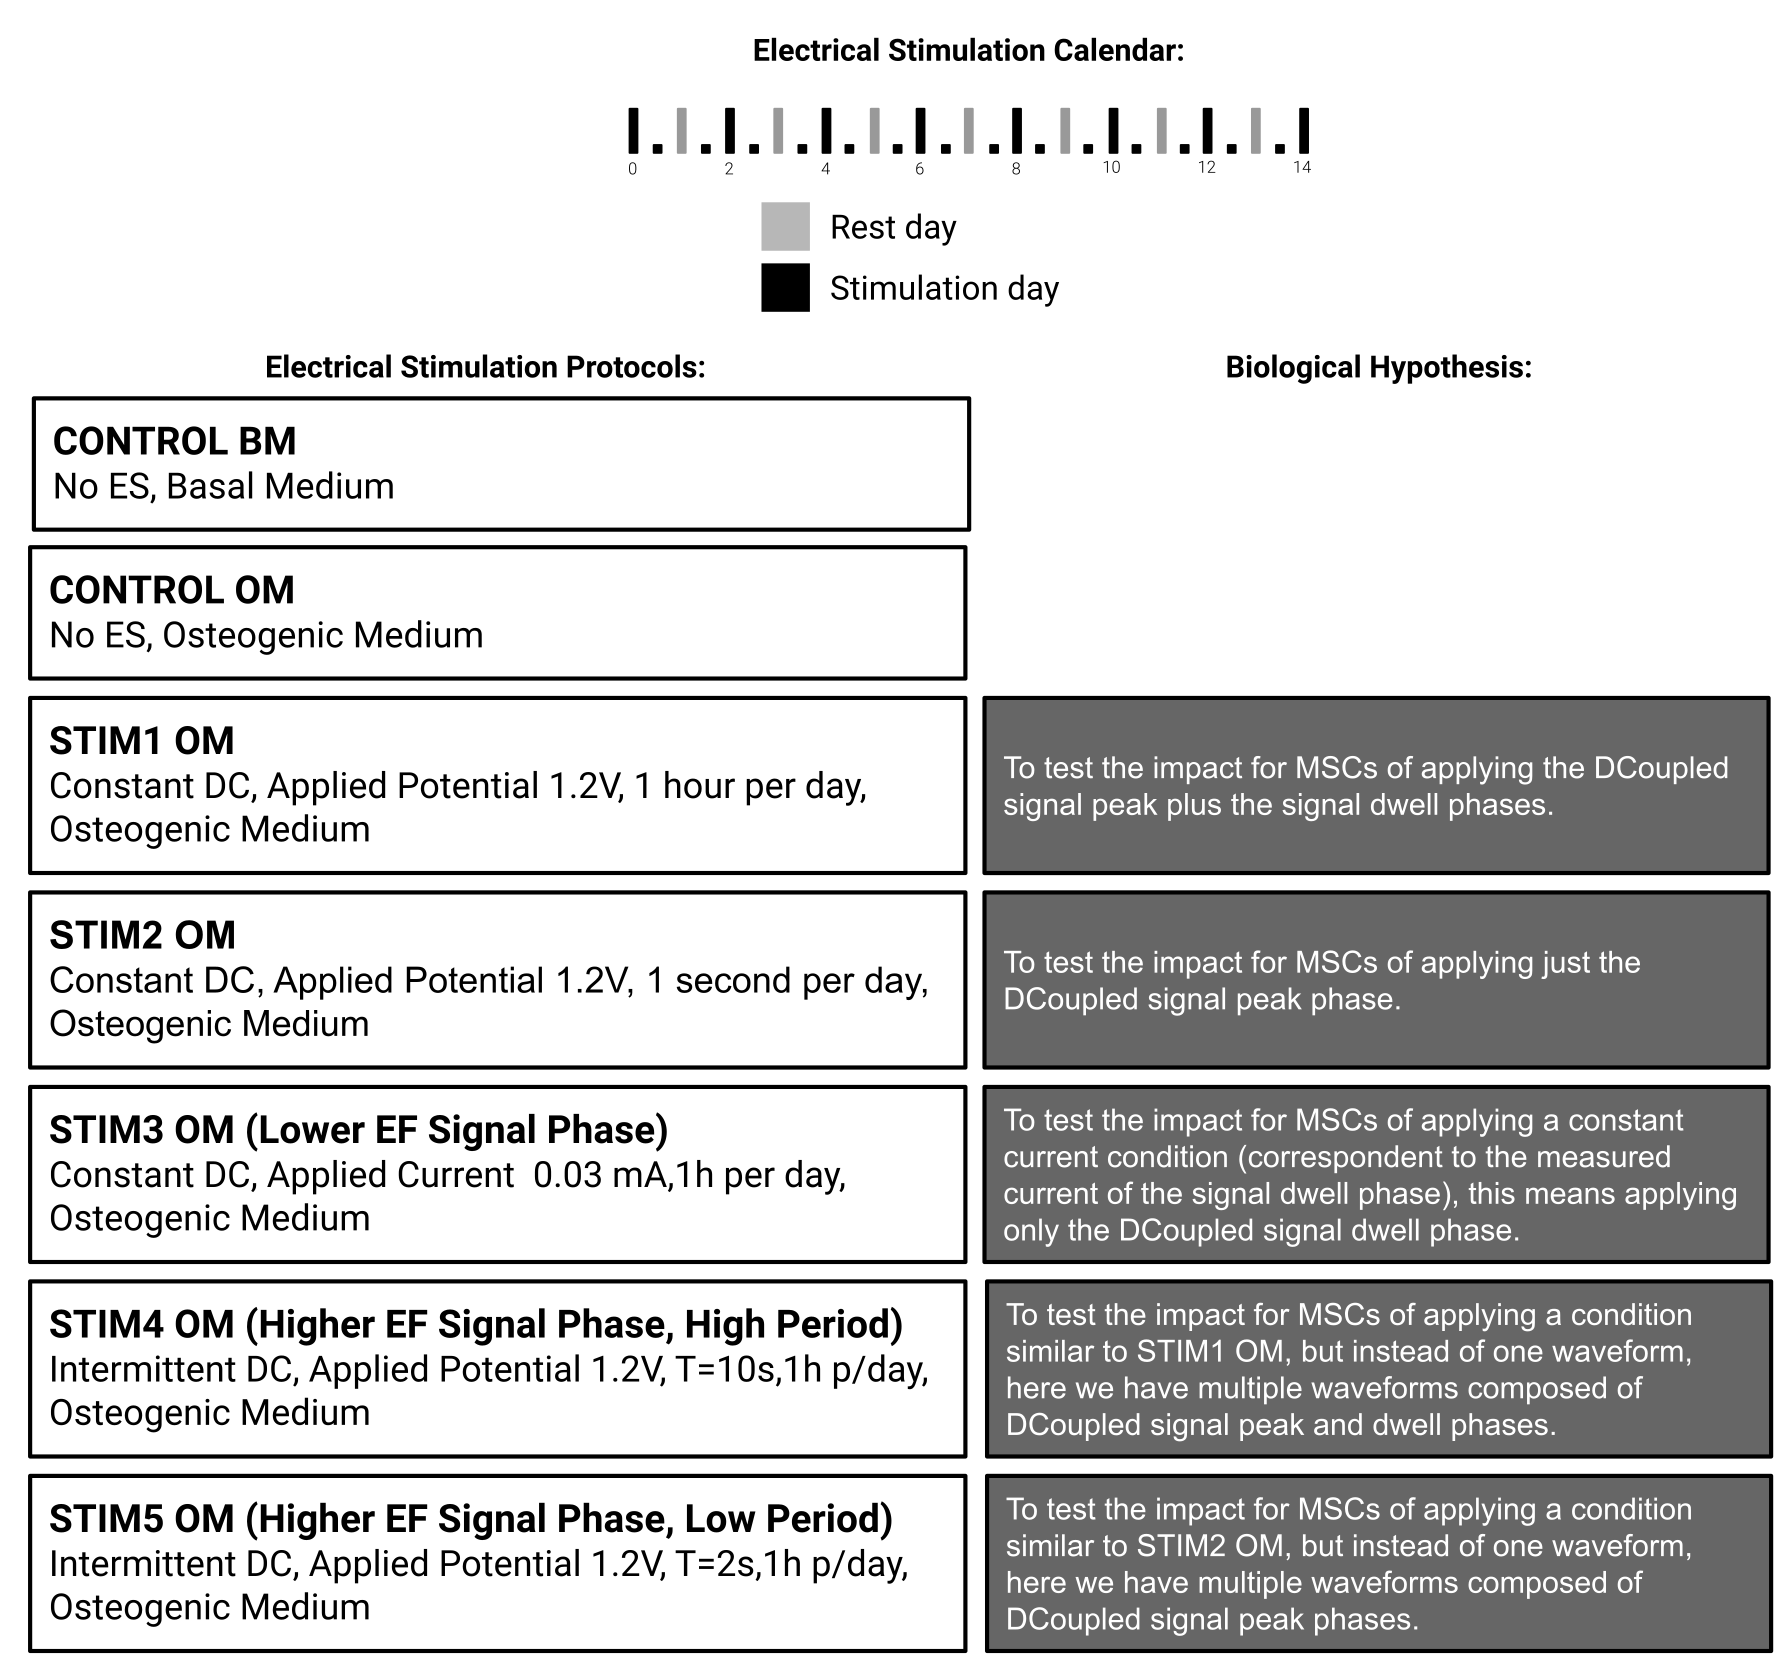
\includegraphics[scale=0.8]{./figures/Table_4d1.png}}
\caption{Infography with DCoupled electrical stimulation protocol description and biological hypothesis under test. Above is the stimulation timeline that was applied to every stimulation condition. Each mentioned protocol reference code will be used in the rest of this chapter to reference a particular protocol.}
\label{fig_t4d1}
\end{figure} 

\subsection{Human \ac{MSCs} culture}
Human bone marrow-derived \ac{MSCs} used in this work were part of the cell bank available at the Stem Cell Engineering Research Group - Institute for Bioengineering and Biosciences (iBB) at Instituto Superior Técnico (IST). Those MSCs were previously isolated according to protocols previously established at iBB-IST \cite{Carvalho2021-ru}. Bone marrow aspirates (Male 46 years) were obtained from Centro Clínico da GNR-Lisboa under previously established collaboration agreements with iBB-IST. An additional sample of fresh, unprocessed bone marrow (Male 24 years) was obtained from Lonza (Switzerland). The human samples were obtained from healthy donors after written informed consent according to Directive 2004/23/EC of the European Parliament and of the Council of March 31, 2004, on setting standards of quality and safety for the donation, procurement, testing, processing, preservation, storage, and distribution of human tissues and cells (Portuguese Law 22/2007, June 29), with the approval of the Ethics Committee of the respective clinical institution. Isolated cells were frozen in liquid/vapor nitrogen tanks until further use. Before the cell culture assays, the \ac{MSCs} were thawed and expanded on tissue culture flasks (T-75 \si{\square\centi\meter}) using low-glucose \acs{DMEM} (Gibco, Thermo Fisher Scientific) supplemented with 10\si{\percent} \acs{FBS} (Gibco, Thermo Fisher Scientific) and 1\si{\percent} Anti-Anti Solution (Gibco, Thermo Fisher Scientific). Cells were kept in an incubator at 37 \si{\celsius} and 5\si{\percent} CO\textsubscript{2} in a humidified atmosphere, and the medium was exchanged every three days. All the experiments were conducted using cells between passages 3 and 5. 

\subsection{Evaluation of the effects of different electric stimulation protocols on MSC proliferation and osteogenic differentiation} 
Human bone marrow-derived \ac{MSCs} were harvested and seeded in 6-well culture plates at a density of 10.000 cells/ \si{\square\centi\meter}. The cells were then cultured for 14 days in an incubator at 37 \si{\celsius} and 5\si{\percent} CO\textsubscript{2} under the different electrical stimulation protocols and respective controls as previously specified in subsection 4.3.6. Culture media (volume of 3 mL per well) were fully renewed every three days. Cell morphology and metabolic activity were monitored throughout the culture after 14 days of culture and exposure to the different electric stimulation protocols, and the osteogenic differentiation of \ac{MSCs} was assessed. 

\subsection{Cell viability and morphology assessment} 
After 14 days of human bone marrow-derived \ac{MSCs} osteogenic differentiation under the different electric stimulation protocols, cell viability was assessed through LIVE/DEAD staining. Briefly, cells were first washed with \ac{PBS}, after which they were incubated in the dark with ethidium bromide (2 \si{\micro\molar}) (Sigma-Aldrich) and calcein (4 \si{\micro\molar}) (Sigma-Aldrich) solution (prepared in \ac{PBS}) for 1 hour. Fluorescence images were obtained using a LEICA DMI3000B inverted fluorescence microscope (Leica Microsystems). 

Cell morphology was observed and imaged at several culture time points using bright-field microscopy (LEICA DMI3000B, Leica Microsystems). At the end of the protocol (day 14), the morphology of the cells was also observed after staining with 4,6-diamidino-2-phenylindole dihydrochloride (DAPI, nuclei stains in blue) and Phalloidin (actin cytoskeleton stains in red). For that, the cultures were firstly washed with \ac{PBS}, fixed in 4\si{\percent} paraformaldehyde (Sigma-Aldrich) solution (in \ac{PBS}) for 20 minutes and permeabilized in a 0.1\si{\percent} Triton X-100 solution (Sigma-Aldrich) in \ac{PBS} for 10 minutes. Afterward, cells were incubated with Phalloidin-TRITC (2 \si{\micro\gram\per\milli\liter} in PBS; Sigma Aldrich) and protected from light for 45 minutes. Samples were then washed with \ac{PBS} and counterstained with DAPI (1.5 \si{\micro\gram\per\milli\liter} in \ac{PBS}; Sigma-Aldrich) for 5 minutes. Finally, the cultures were rewashed with PBS, and the fluorescence staining was imaged using an inverted fluorescence microscope (LEICA DMI3000B, Leica Microsystems). 

\subsection{Metabolic activity assay} 
The metabolic activity of differentiating human bone marrow-derived \ac{MSCs} under the different electric stimulation protocols (and respective controls) was evaluated on days 3, 7, and 14 using the AlamarBlue assay (AlamarBlue Cell Viability Reagent; Thermo Fisher Scientific) following the manufacturer’s guidelines. Briefly, a 10\si{\percent} (v/v) AlamarBlue solution diluted in cell culture media was added to the cell cultures and incubated at 37 \si{\celsius} and 5\si{\percent} CO\textsubscript{2} in a humidified atmosphere for 3 \si{\hour}. Fluorescence intensity was measured in a microplate reader (Infinite 200 Pro; TECAN) at an excitation/emission wavelength of 560/590 \si{\nano\meter}. For each experimental group, the fluorescence intensity was analyzed in 3 independent samples ($n=3$), and the fluorescence values of each sample were measured in triplicates. 

\subsection{Alkaline phosphatase activity assay} 
\acs{ALP} activity, which is associated with bone formation and osteoblast function \cite{Nakamura2020-zx}, was quantified using a colorimetric \ac{ALP} quantification kit (BioAssays Systems) following the manufacturer’s guidelines. \ac{ALP} activity was assessed after 14 days of osteogenic differentiation under the different electric stimulation protocols. Cultures were firstly washed with \ac{PBS}, and lysates were obtained after incubation in a 0.2\si{\percent} Triton X-100 (Sigma-Aldrich) solution (prepared in \ac{PBS}) overnight at room temperature and under agitation. Afterward, a p-nitrophenyl solution (10 \si{\milli\molar}) was added to the lysates. The absorbance was measured on a microplate reader (Infinite 200 Pro; TECAN) at 405 \si{\nano\meter}. For each experimental group, the absorbance was quantified for three independent samples ($n=3$), and values for each sample were measured in triplicates. \ac{ALP} activity values were calculated following the manufacturer’s protocol and normalized to the cell metabolic activity of each sample.  

\subsection{Calcium quantification assay} 
The calcium content levels produced by human bone marrow-derived \ac{MSCs} under osteogenic differentiation and submitted to the different electric stimulation protocols for 14 days were determined using a calcium colorimetric assay kit (Sigma-Aldrich). First, cells were washed with \ac{PBS} and incubated in a 1\si{\molar} HCl solution overnight (with agitation). Afterward, the supernatant was collected and used for calcium determination, following the manufacturer’s instructions. Briefly, three independent samples of each experimental condition ($n=3$) and diluted forms of a Calcium Standard Solution (500 \si{\milli\molar}) available in the kit were pipetted into a 96-well plate at several concentrations. Afterward, a Chromogenic Reagent and a Calcium Assay buffer (provided in the kit) were added to each well, and the solutions were gently mixed. The samples were incubated for 10 min in the dark at room temperature. The absorbance was measured on a microplate reader (Infinite 200 Pro; TECAN) at 575 \si{\nano\meter} (duplicate measurements per sample). The absorbance measurements for the different Calcium Standard Solution concentrations were used to develop a calibration curve, which was used to estimate the concentration of calcium present in each sample. The values were normalized to the cell metabolic activity of the respective sample.

\subsection{Osteogenic stainings} 
\ac{ALP}/Von Kossa, Alizarin Red, and Xylenol Orange stainings are often used to confirm the osteogenic differentiation of \ac{MSCs} through the detection of the bone \ac{ECM} markers (\ac{ALP} and mineral deposits) \cite{Zhou2021-av}. In this study, the stainings were performed after 14 days of osteogenic differentiation under the different electric stimulation protocols. After being washed with \ac{PBS} and fixed with 4\si{\percent} paraformaldehyde for 20 min, the human bone marrow-derived \ac{MSCs} were first washed twice with milliQ and stained for ALP presence by incubation in a solution comprised of 0.1 \si{\molar} TRIS-HCl (Sigma-Aldrich), containing Fast Violet Solution (Sigma-Aldrich) and Naphthol AS MX-P04 (Sigma-Aldrich) for 45 min. The cells were then washed three times with \ac{PBS} and kept in milliQ water while being observed under the microscope (LEICA DMI3000B, Leica Microsystems). After washing the samples with \ac{PBS}, Von Kossa staining was performed on the same samples by incubating them in a 2.5\si{\percent} silver nitrate solution (Sigma-Aldrich) for 30 min. Finally, the cultures were washed three times with \ac{PBS}, once with miliQ water, and kept in milliQ water until observation under the microscope (LEICA DMI3000B). 

Alizarin red staining of the cells from different experimental groups was performed to detect the calcium deposits. Paraformaldehyde-fixed samples were incubated in a 2\si{\percent} Alizarin red (Sigma-Aldrich) solution (in \ac{PBS}) for 1 hour at room temperature. The cultures were washed afterward multiple times with \ac{PBS} and milliQ water, after which they were imaged with an inverted fluorescence microscope (LEICA DMI3000B).  

To further confirm the presence of mineral deposits within the samples after 14 days of human bone marrow-derived \ac{MSCs} osteogenic differentiation under the different electric stimulation protocols, a 20 \si{\milli\molar} Xylenol Orange solution (Sigma-Aldrich) was added to previously fixed samples for 1 hour at room temperature. Cells were then washed successively with \ac{PBS}, and the fluorescence staining was imaged using an inverted fluorescence microscope (LEICA DMI3000B).

\subsection{\acs{RNA} isolation, conversion to complementary \acs{DNA}, and quantitative real-time polymerase chain reaction (\acs{RT-qPCR}) analysis} 

After the osteogenic differentiation of human bone marrow-derived \ac{MSCs} under the different electric stimulation protocols for 14 days, cells were harvested from the plates, centrifuged, and the obtained pellets were stored at -80 \si{\celsius} until further use. \ac{RNA} extraction from cell pellets was performed using the RNeasy Mini Kit (QIAGEN) according to the manufacturer’s guidelines. Afterwards, the \ac{RNA} concentration of the different samples was quantified using a NanoVue Plus spectrophotometer (GE Healthcare).  

Complementary \ac{DNA} was synthesized from the purified \ac{RNA} using the High-Capacity complementary \ac{DNA} Reverse Transcription Kit (Applied Biosystems) according to the manufacturer’s protocol. Reaction mixtures comprised of 10 \si{\micro\liter} of MasterMix – constituted by 2 \si{\micro\liter} of RT 10x buffer, 0.8 \si{\micro\liter} of dNTP mix, 4.2 \si{\micro\liter} of RNase-free water, 2 \si{\micro\liter} of random primers and 1 \si{\micro\liter} of Multiscribe Reverse Transcriptase – and 10 \si{\micro\liter} of purified \ac{RNA} sample were mixed and placed in a T100TM thermal cycler (Bio-Rad) for 5 minutes at 25 \si{\celsius}, 20 minutes at 46 \si{\celsius} and 1 minute at 95 \si{\celsius}, and then were maintained at 4 \si{\celsius}.  

\acs{RT-qPCR} analysis was performed using a StepOnePlus real-time polymerase chain reaction system (Applied Biosystems) and NZYSpeedy qPCR Green Master Mix (2x), ROX plus (Nzytech) following the manufacturer’s protocol. The reactions were carried out at 95 \si{\celsius} for 10 minutes, followed by 40 cycles of 95 \si{\celsius} for 15 seconds and 60 \si{\celsius} for 1 minute. All samples were analyzed in triplicates ($n=3$). The results obtained were analyzed using the 2-\si{\Delta\Delta}Ct method to determine relative changes in specific target genes (ALP, RUNX2, COL1A1, OPN, OC, CACNA1C, and SCN1\si{\alpha}) expression compared with the control sample (human bone marrow-derived \ac{MSCs} at day 0 before seeding). Gene expression was primarily normalized to the housekeeping gene glyceraldehyde-3-phosphate (GADPH) expression and then calculated as a fold-change relative to the baseline expression of the target genes in the control sample. The primer sequences used in the \ac{RT-qPCR} analysis are presented in Table \ref{tabPrimers}.

\begin{table}
\caption{Primer sequences used in the RT-qPCR analysis.}
\bigskip
\scriptsize
\centering
\begin{tabularx}{350px}{lll} \toprule[0.25em]
\multicolumn{1}{l}{\textbf{GENE}} & \textbf{FWD PRIMER SEQUENCE} & \textbf{REV PRIMER SEQUENCE} \\ \cmidrule(r){1-3}
GAPDH & \textit{5’-GGTCACCAGGGCTGCTTTTA-3’} & \textit{5’-CCTGGAAGATGGTGATGGGA -3’} \\
ALP & \textit{5’- ACCATTCCCACGTCTTCACATTT-3’} & \textit{5’- AGACATTCTCTCGTTCACCGCC-3’} \\
Runx2 & \textit{5’-AGATGATGACACTGCCACCTCTG-3’} & \textit{5’-GGGATGAAATGCTTGGGAACT-3’} \\
COL1A1 & \textit{5’-CATCTCCCCTTCGTTTTTGA-3’} & \textit{5’-CCAAATCCGATGTTTCTGCT-3’} \\
OPN & \textit{5’-CAGGTCTGCGAAACTTCTTAG-3’} & \textit{5’-CTCCATTGACTCGAACGACTC-3’} \\
OC & \textit{5’-TGTGAGCTCAATCCGGCATGT-3’} & \textit{5’-CCGATAGGCCTCCTGAAGC-3’} \\
CACNA1C & \textit{5’-GTACAAAGACGGGGAGGTTGAC-3’} & \textit{5’-GTAGTTGTAGATGGGGCCCTTG-3’} \\
SCN1\si{\alpha} & \textit{5’- TTGTGACGCTTAGCCTGGTAG-3’} & \textit{5’- ACGATGATGGCCAAGACGAG-3’} \\ \bottomrule[0.25em] 
\end{tabularx}
\label{tabPrimers}
\end{table} 

\subsection{Immunofluorescence analysis of bone-specific proteins} 
Immunofluorescence analysis evaluated the presence of type I collagen, osteopontin, and osteocalcin (relevant proteins produced during bone \acs{ECM} formation) within the cultures after 14 days of osteogenic differentiation under the different electric stimulation protocols. Previously fixed (paraformaldehyde 4\si{\percent} for 20 minutes) samples were washed twice in \acs{PBS}, after which the scaffolds were immersed in a permeabilization/blocking solution comprised of 1\si{\percent} \ac{BSA} (Sigma-Aldrich), 10\si{\percent} \acs{FBS} and 0.03\si{\percent} Triton X-100 for 45 min at room temperature. Solutions containing primary antibodies for type I collagen (MA1-26771, Thermo-Fischer), osteopontin (ab8448, Abcam) and osteocalcin (MAB1419, R\&D Systems) (1:200 in 1\si{\percent} \acs{BSA}, 10\si{\percent} \acs{FBS}, 0.03\si{\percent} Triton X-100 solution) were then incubated with the respective samples overnight at 4 \si{\celsius}. Cells were then incubated with the secondary antibodies (1:200 in 1\si{\percent} \acs{BSA}; goat anti-mouse IgG-AlexaFluor 546 (Thermo Fisher Scientific) for type I collagen and goat anti-rabbit IgG-AlexaFluor 546 (Thermo Fisher Scientific) for osteopontin and osteocalcin) for 1 hour at room temperature in the dark. Following two washes with \ac{PBS}, the samples were counterstained with DAPI (1.5 \si{\micro\gram\per\milli\liter} in \ac{PBS}) for 5 min at room temperature, washed twice with \ac{PBS} and imaged using a fluorescence microscope (LEICA DMI3000B). 

\subsection{Statistical analysis}
When applicable, results are presented as average values $\pm$ standard deviation (SD). All the in vitro cell culture experiments were performed using three independent samples ($n=3$) from two different donors unless specified otherwise. Statistical analysis of the data was performed by one-way ANOVA, followed by a Tukey post-hoc test using the GraphPad Prism 7.0 software (GraphPad, San Diego, CA, USA). Data were considered statistically significant when the p-values obtained were less than 0.05 (95\si{\percent} confidence intervals, $*p<0.05$). 




\section{Results}


\subsection{Electrode/electrolyte interface characterization}
The response of a DCoupled system single well (filled with osteogenic culture medium) to an electric current square wave input followed the predicted response for a faradaic process. Such behavior differs from a typical non-faradaic process, as shown in Figure \ref{fig4d4}a,b. Moreover, replacing the osteogenic culture medium with basal medium resulted in the same response curve shape, meaning that a faradaic process also drives basal medium interaction with stainless steel wire 316LVM. We further confirmed the electrode/electrolyte interface faradaic process by analyzing the response to an electric potential step, since the response curve shape followed exactly the waveform indicated by Biesheuvel \textit{et al.} \cite{Biesheuvel2018-wu} (Figure \ref{fig4d4}c). This potential step response curve is characterized by an initial signal peak (higher potential and current) when the input potential step is applied, followed by a decrease in the electric potential until it reaches a stable signal dwell (lower potential and current). The developed system, composed of a series of three wells, showed the same response (Figure \ref{fig4d5}a), attenuated by the fact that the overall electric resistance of the system is at least three times higher than the electric resistance of a single well. The I-V curve for these three wells in a series setup is also shown in Figure \ref{fig4d5}b. We digitized the curve obtained by Srirussamee \textit{et al.} \cite{Srirussamee2021-cj} (red line in Figure \ref{fig4d5}b) and observed that our stable curve and theirs are similar in shape. The divergence observed in the values may be attributed to the different electrode/electrolyte species involved. We clarify that the stable curve in Figure \ref{fig4d5}b represents the value of the electric current in the signal dwell phase. In contrast, the peak curve represents the maximum current achieved when the input signal is applied to the three wells in the series setup. The applied potential of 1.2 \si{\volt} was chosen deliberately below the water electrolysis limit of 1.23 \si{\volt} \cite{Guette-Marquet2021-rp} to test if DCoupled electric stimulation performed below the water electrolysis potential remains capable of producing similar osteoinductive effects as previously reported at higher potentials \cite{Mobini2017-wp, Mobini2017-zr, Leppik2018-bw}. When 1.2 \si{\volt} is applied to our setup, we measured a peak electric current of 0.17 \si{\milli\ampere} (during signal peak) preceding a current drop to 0.02 - 0.03 \si{\milli\ampere} (during signal dwell). Dwell current showed to be slowly dropping with time. Regarding the electric current controlled hypothesis, a constant current condition of 0.03 \si{\milli\ampere} generated electrode potential differences that grew above the water electrolysis limit, registering a maximum potential difference of 3.74 \si{\volt} for one electrode pair in a three-well series. The results from this characterization process allowed us to create the protocol conditions described in the methods section, disaggregating the part of the waveform responsible for the higher current and higher \acs{EF} from the part responsible for the lower current and lower \acs{EF}.    

\begin{sidewaysfigure}
\makebox[\textwidth][c]{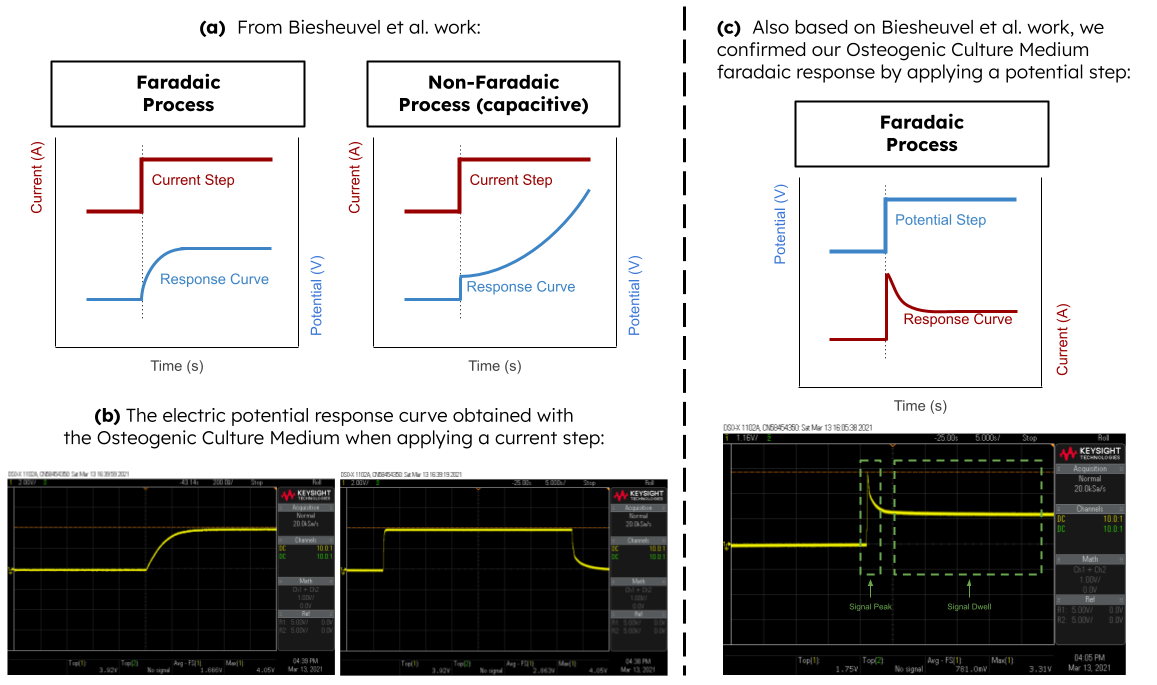
\includegraphics[scale=0.50]{./figures/Figure_4d4.png}}
\caption{Responce characterization of a DCoupled system accordingly to Biesheuvel \textit{et al.} \cite{Biesheuvel2018-wu}: (a) Reference Faradaic versus Non-Faradaic expected responses for an applied current step; (b) Oscilloscope print screens for the measured responses of the custom developed DCoupled system for a current step input, showing a Faradaic process response. At the vertical axis is presented the electric potential and at the horizontal axis is the time; (c) Reference versus oscilloscope print screen for the measured responses of the custom-developed DCoupled system for a potential step input. In the potential step response (c), the peak and dwell phases of the waveform are identified.}
\label{fig4d4}
\end{sidewaysfigure}

\begin{sidewaysfigure}
\makebox[\textwidth][c]{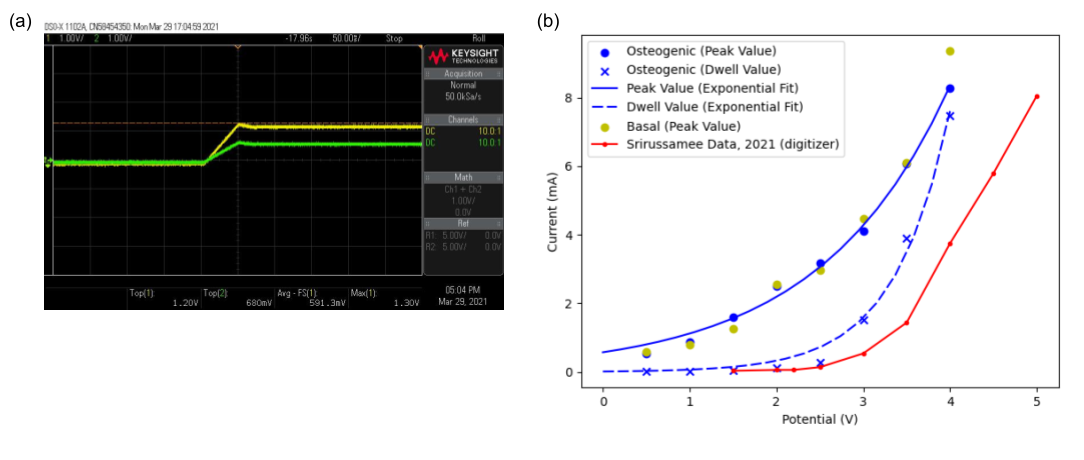
\includegraphics[scale=0.50]{./figures/Figure_4d5.png}}
\caption{Response of the developed DCoupled setup with three wells in series: (a) Oscilloscope print screen for the potential step input response. It shows the measurements at the first (yellow curve) and last electrode (green curve) in the three wells array; (b) Comparison between the obtained I-V curve (maximum and stable forms, in blue) and curve data from Srirussamee \textit{et al.} \cite{Srirussamee2021-cj} (in red; obtained with a digitizer).}
\label{fig4d5}
\end{sidewaysfigure}


\subsection{Computational modelling of the \acs{EF}}
Before the \acs{FEM} analysis of the \acs{EF}s generated within the electric stimulation setup, the electrical conductivities of both basal (BM) and osteogenic (OM) culture media were determined. For typical room temperatures of 21 - 23 \si{\celsius}, the electrical conductivity values were 1.383 \si{\siemens\per\meter} (OM) and 1.392 \si{\siemens\per\meter} (BM). Increasing the media temperature to 37 \si{\celsius} also increased its electrical conductivity to 1.741 \si{\siemens\per\meter} (OM) and 1.725 \si{\siemens\per\meter} (BM). The values measured follow the ones reported by Mazzoleni \textit{et al} \cite{Mazzoleni1986-wp}. 

\ac{FEM} solutions were obtained using the conjugate gradients iterative solver, that quickly converged (less than 10s). Mesh independence was confirmed by repeating the calculation of the obtained results with the COMSOL extremely fine element size option. Slight geometrical deviations were introduced into the developed model to study the impact of such differences in the \acs{EF} magnitude. Changing the distance between electrodes from 20  to 25 \si{\milli\meter} (while keeping the culture medium volume height constant and a constant electric current input) showed no difference in the \acs{EF} predictions larger than 0.01 \si{\volt\per\meter}, stating that minor geometric deviations do not impact on this particular setup. The impact of culture media height changes was also studied (ranging from 2 \si{\milli\meter} to 6 \si{\milli\meter} in steps of 1 \si{\milli\meter}) at the same constant electric current magnitude and distance between the electrodes. The predicted \acs{EF} changes by almost 30\si{\percent} per milliliter of culture medium added or removed. This result indicates that each well should have the same volume of culture medium. In this study, we used 3 \si{\milli\liter} of culture medium per well of a standard 6-well culture plate, corresponding to a height of approximately 3.5 \si{\milli\meter}. At a constant electric current and culture medium height, changing the electrode length to more or less 5 \si{\milli\meter} will have a maximum impact of 6\si{\percent} in the predicted \acs{EF}. Also, under the same conditions, twisting 5\si{\degree} up/down one or both electrodes corresponds to a maximum variation of 0.09\si{\percent} in the predicted \acs{EF}, representing only a residual impact in this setup (Tables \ref{tab4d1},\ref{tab4d2},\ref{tab4d3}). Our modelling method applied to Mobini \textit{et al.} \cite{Mobini2016-jh} setup predicts an average \acs{EF} in the cell culture medium of 0.59 \si{\volt\per\meter}. The solution converged in 2 seconds, and as previously stated in the methods section, it considered the resulting current of 0.07 \si{\milli\ampere} as reported by Srirussamee \textit{et al.} \cite{Srirussamee2019-ai} and geometry approximations as reported in the original Mobini \textit{et al.} manuscript. 

Numerical \ac{FEM} models of the developed setup predicted an average culture medium \acs{EF} in each of the three wells of 1.48 \si{\volt\per\meter} during the signal peak phase and 0.26 \si{\volt\per\meter} during the signal dwell phase (Figure \ref{fig4d6}a, \ref{fig4d6}b).


\begin{figure}
\makebox[\textwidth][c]{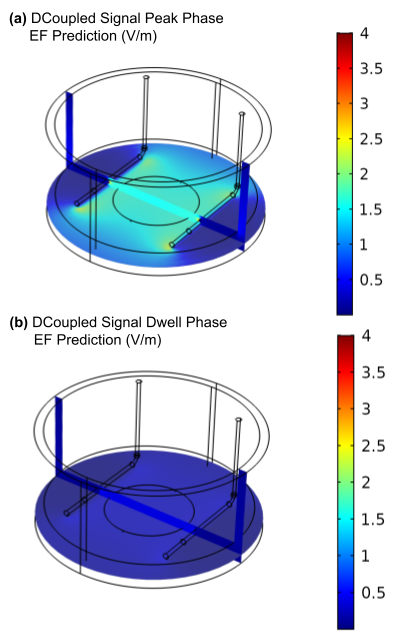
\includegraphics[scale=0.65]{./figures/Figure_4d6.png}}
\caption{FEM numerical model of the developed DCoupled setup: (a) EF prediction for the signal peak electric current of 0.17 \si{\milli\ampere}; (b) EF prediction for the signal dwell electric current of 0.03 \si{\milli\ampere}.}
\label{fig4d6}
\end{figure}

\begin{table}
\caption{Predicted impact of electrodes distance in the DCoupled setup \acs{EF} stimulation delivery at the \acs{ROI}, considering 2 \si{\milli\meter} of culture medium height, 20/25 \si{\milli\meter} distance.}
\bigskip
\small
\centering
\begin{tabularx}{280px}{lll} \toprule[0.15em]
 \textbf{Distance Between Electrodes} & \multicolumn{2}{l}{\textbf{Electric Field}} \\ \cmidrule(l){2-3}
 & 0.03 \si{\milli\ampere} & 0.17 \si{\milli\ampere} \\ \cmidrule(r){1-3}
25 \si{\milli\meter}  & 0.33 \si{\volt\per\meter} & 1.88 \si{\volt\per\meter} \\
20 \si{\milli\meter}  & 0.33 \si{\volt\per\meter} & 1.88 \si{\volt\per\meter} \\ \bottomrule[0.15em] 
\end{tabularx}
\label{tab4d1}
\end{table}


\begin{table}
\caption{Well liquid volume variation impact in the DCoupled setup \acs{EF} stimulation delivery at the \acs{ROI}, for a constant electric current of 0.05 \si{\milli\ampere}. The green values indicate the variation in the \acs{EF} due to liquid volume change. In contrast, the red values indicate the variation imposed by the longer versus shorter electrodes ($\pm$ 5 \si{\milli\meter} size).}
\bigskip
\small
\centering
\begin{tabularx}{\textwidth}{lll} \toprule[0.25em]
 \textbf{Liquid Height} &  \textbf{Electric Field, Long Electrodes} &  \textbf{Electric Field, Short Electrodes} \\ \cmidrule(r){1-3}
2 \si{\milli\meter} & 0.55 \si{\volt\per\meter} & 0.58 V/m (\textcolor{red}{+5\%}) \\ 
3 \si{\milli\meter} & 0.37 \si{\volt\per\meter} (\textcolor{green}{-32\%}) & 0.38 V/m (\textcolor{red}{+3\%}) \\ 
4 \si{\milli\meter} & 0.27 \si{\volt\per\meter} (\textcolor{green}{-27\%}) & 0.28 \si{\volt\per\meter} (\textcolor{red}{+4\%}) \\ 
5 \si{\milli\meter} & 0.22 \si{\volt\per\meter} (\textcolor{green}{-18\%}) & 0.23 \si{\volt\per\meter} (\textcolor{red}{+5\%}) \\ 
6 \si{\milli\meter} & 0.18 \si{\volt\per\meter} (\textcolor{green}{-18\%}) & 0.19 \si{\volt\per\meter} (\textcolor{red}{+6\%}) \\ \bottomrule[0.25em] 
\end{tabularx}
\label{tab4d2}
\end{table}


\begin{table}
\caption{Worst case scenario impact in the DCoupled setup \acs{EF} stimulation delivery at the \acs{ROI}, considering a twist angle 5º up/down and a constant 5 \si{\milli\meter} culture medium height. The variation value, presented by the red color, was calculated by comparison with the no-twist scenario under the same conditions.}
\bigskip
\small
\centering
\begin{tabularx}{200px}{ll} \toprule[0.15em]
\textbf{Electric Current} &  \textbf{Electric Field}  \\ \cmidrule(r){1-2}
0.03 \si{\milli\ampere} & 0.133 \si{\volt\per\meter} (\textcolor{red}{0.09\%}) \\ 
0.17 \si{\milli\ampere} & 0.75 \si{\volt\per\meter} (\textcolor{red}{0.09\%})  \\ \bottomrule[0.15em] 
\end{tabularx}
\label{tab4d3}
\end{table}



\subsection{Effects of electric stimulation protocols on \ac{MSCs} viability, morphology and proliferation}
The metabolic activity and viability of differentiating human bone marrow-derived \ac{MSCs} cultured under the different electric stimulation protocols for 14 days were evaluated using the AlamarBlue and LIVE/DEAD assays, respectively. As observed in Figure \ref{figMetabolic}A, all electric stimulation conditions promoted the maintenance of high metabolic activities throughout all the analyzed time points, similarly to the non-stimulated controls. However, statistical differences in cells’ metabolic activity were observed between the protocols, particularly on day 14 and concerning protocol STIM3 OM (current control condition). Additionally, all electric stimulation protocols resulted in cultures with high cell viability (the presence of dead cells was residual) and regular morphology, as demonstrated by LIVE/DEAD and DAPI/Phalloidin stainings, respectively (Figure \ref{fig4d7}B). 


\begin{sidewaysfigure}
\makebox[\textwidth][c]{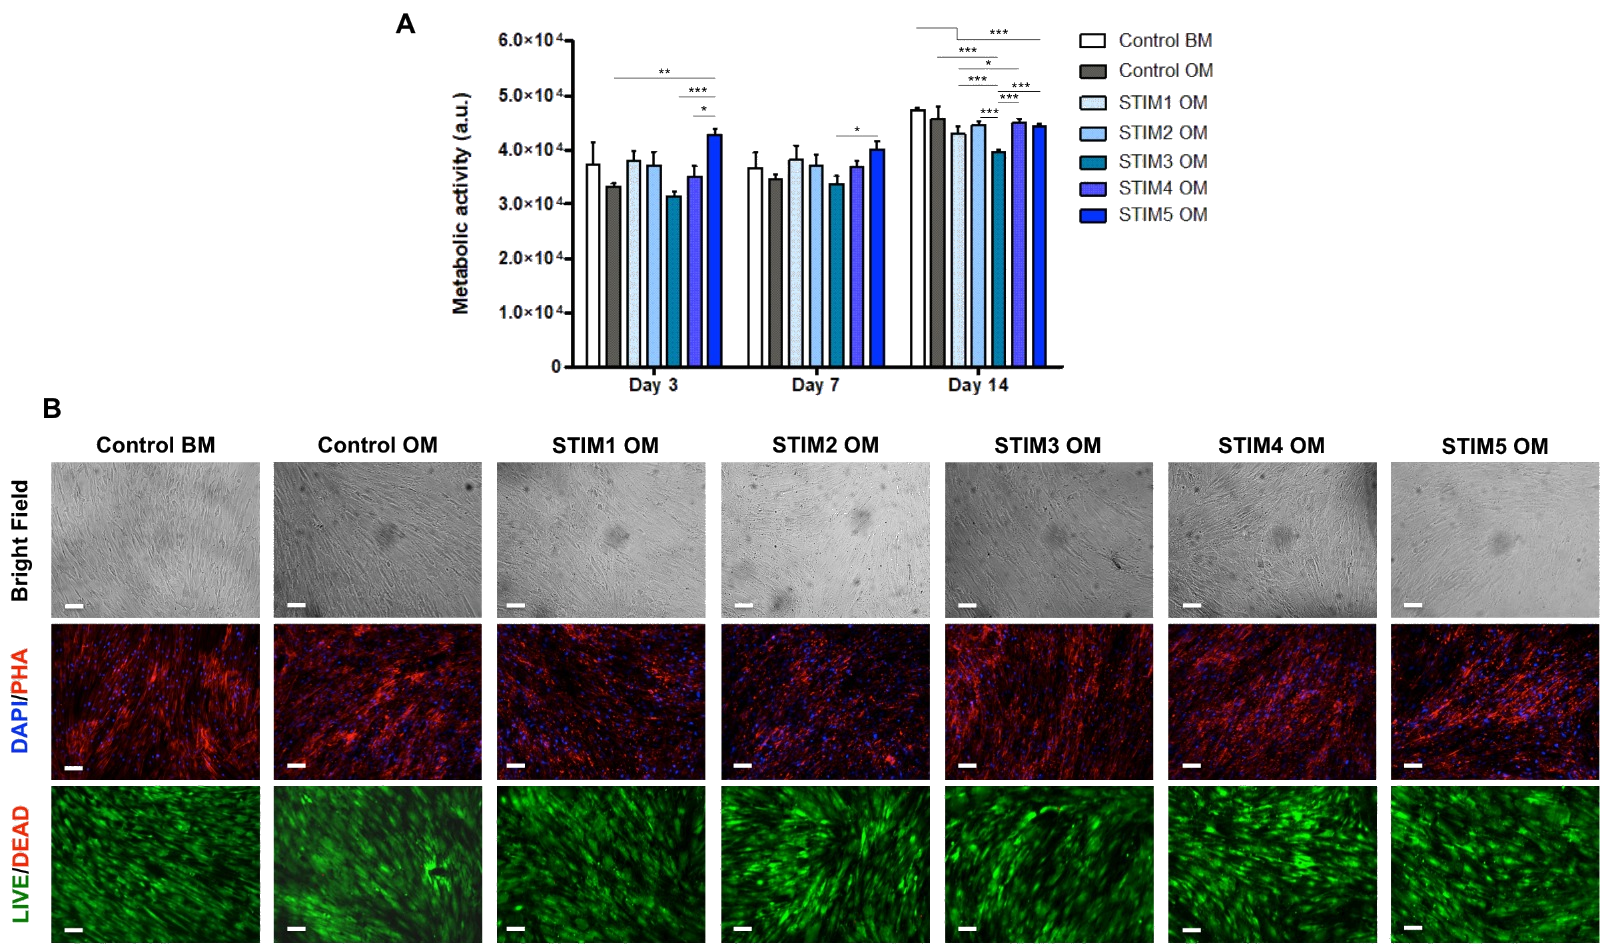
\includegraphics[scale=1.2]{./figures/Figure_4d7.png}}
\caption{Effects of the different electric stimulation protocols on human bone marrow-derived \ac{MSCs} metabolic activity, viability, and morphology. (A) Metabolic activities (determined using the AlamarBlue assay at days 3, 7, and 14) of human bone marrow-derived \ac{MSCs} undergoing osteogenic differentiation under the different electric stimulation protocols. Results are presented as average $\pm$ SD of three ($n=3$) independent experiments. $*p < 0.05; **p < 0.01; ***p < 0.001$. (B) Assessment of cell morphology and viability by Bright Field imaging (top), DAPI/Phalloidin (middle), and LIVE/DEAD (bottom) fluorescent stainings at the end of the experiment (day 14). DAPI stains the nuclei blue, and Phallodin stains the actin cytoskeleton red. In the LIVE/DEAD staining, viable cells are stained in green, while dead cells appear in red. Scale bar: 100 \si{\micro\meter}.}
\label{fig4d7}
\end{sidewaysfigure}
 

\subsection{\acs{ALP} activity, calcium production, and osteogenic stainings} 
To assess the effects of the different electric stimulation protocols on the osteogenic differentiation of human bone marrow-derived \ac{MSCs}, \acs{ALP} activity (Figure \ref{fig4d8}A) and calcium content (Figure \ref{fig4d8}B) quantitative assays were performed on the cultures obtained at the end of the experiment (day 14). As expected, all the conditions (electrically stimulated and non-stimulated) cultured under osteogenic medium presented statistically significant higher \ac{ALP} activities in comparison to the non-stimulated cells cultured under standard growth media conditions (CONTROL BM). Lower \ac{ALP} activity values were observed for the current-based protocol (STIM 3 OM). Nevertheless, this difference was not statistically significant (Figure \ref{fig4d8}A). 

Regarding mineralization, the experimental groups cultured under osteogenic induction conditions present significantly higher calcium contents than the CONTROL BM group (Figure \ref{fig4d8}B). Notably, the current-based electric stimulation protocol (STIM 3 OM) was the only condition that achieved statistically significant higher calcium content (mineralization) than the non-stimulated cells cultured under osteogenic medium (CONTROL OM).

\begin{figure}
\makebox[\textwidth][c]{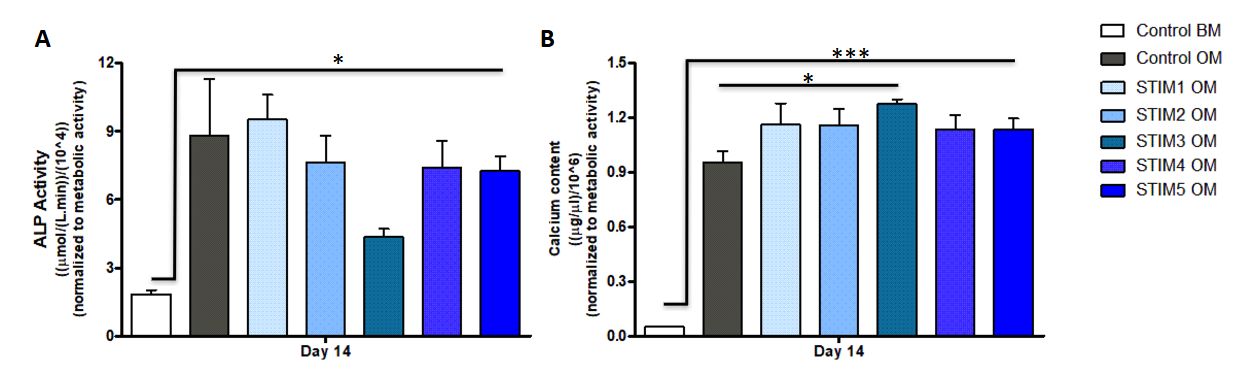
\includegraphics[scale=0.50]{./figures/Figure_4d8.png}}
\caption{(A) \ac{ALP} activity and (B) calcium deposition quantification of human bone marrow-derived \ac{MSCs} cultured under five different electric stimulation protocols after 14 days of osteogenic differentiation. Results are presented as average $\pm$ SD of three ($n=3$) independent experiments. $*p < 0.05; ***p < 0.001$.}
\label{fig4d8}
\end{figure}

The differentiation of human bone marrow-derived \ac{MSCs} towards osteoblasts was further confirmed by the common ALP/Von Kossa, Alizarin Red, and Xylenol Orange osteogenic stainings (Figure \ref{fig4d9}). As expected, all the experimental groups cultured under osteogenic induction medium stained positively for \ac{ALP} activity (top row) and cell mineralization (three bottom rows), demonstrated by the presence of black, red, and fluorescent red mineralized deposits identified by Von Kossa, Alizarin Red and Xylenol Orange stainings, respectively. None or minimal positive osteogenic stainings were observed for the CONTROL BM group. Importantly, all the electric stimulation protocols showed a more intense and spread staining concerning the Alizarin Red staining than the osteogenic non-stimulated group (CONTROL OM). This was particularly evident for the STIM1 OM and STIM3 OM experimental groups. Moreover, Xylenol Orange staining images also suggest a more intense staining for the current-controlled protocol (STIM3 OM).

\begin{sidewaysfigure}
\makebox[\textwidth][c]{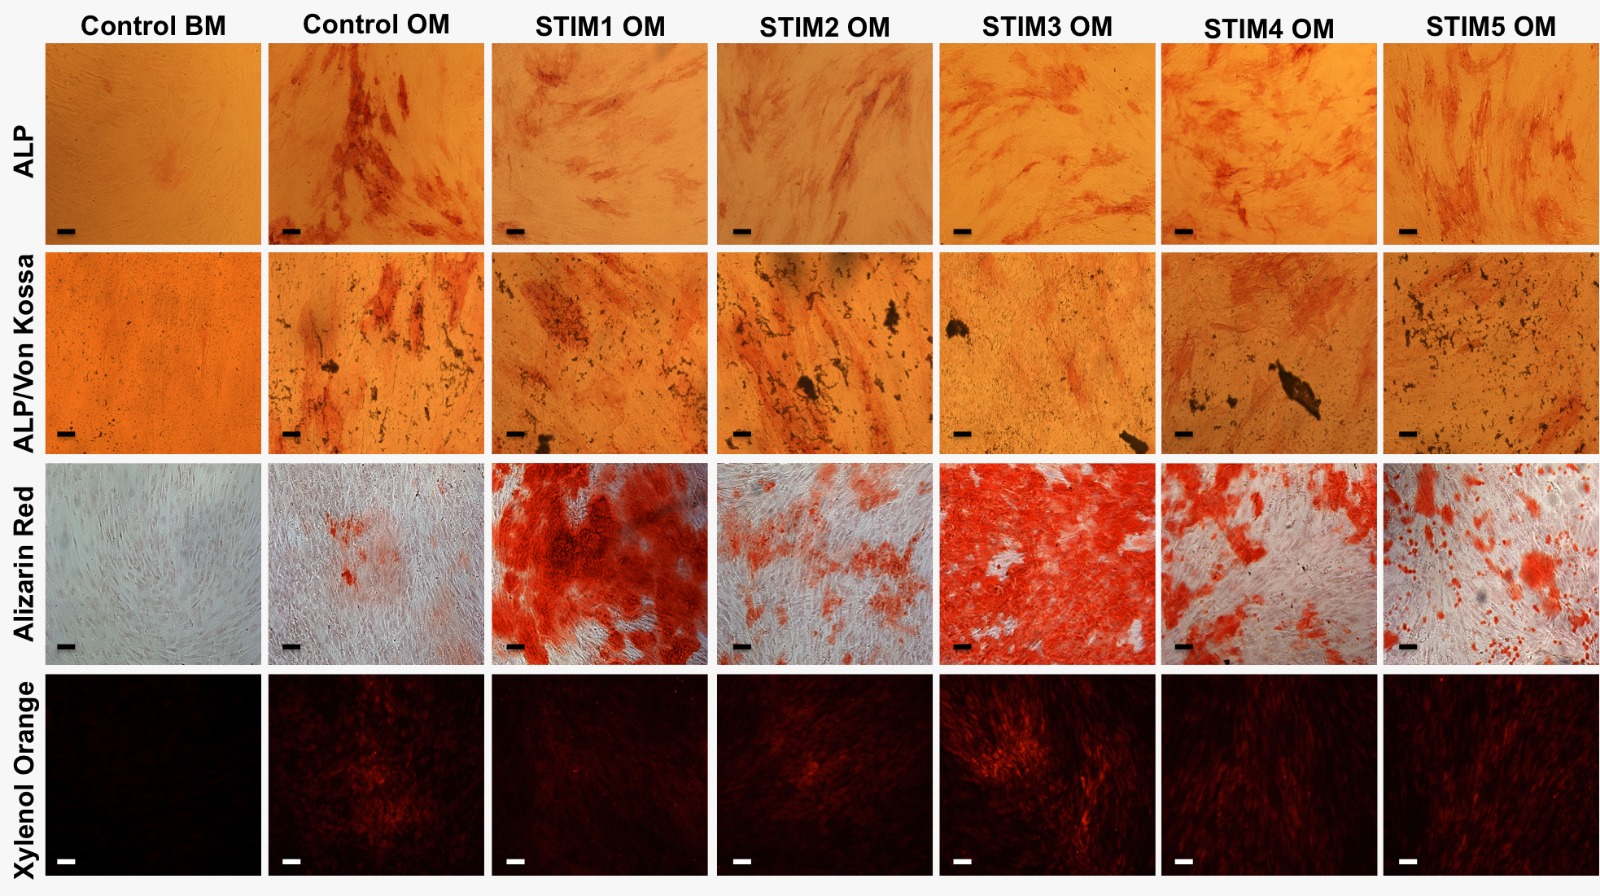
\includegraphics[scale=0.35]{./figures/Figure_4d9.jpeg}}
\caption{ALP, ALP/Von Kossa, Alizarin Red, and Xylenol Orange stainings (from top to bottom rows) of human bone marrow-derived \ac{MSCs} cultured under osteogenic differentiation conditions and exposed to the different electric stimulation protocols for 14 days (and respective non-stimulated controls). \acs{ALP}/Von Kossa staining evidenced the \ac{ALP} activity of the differentiating human bone marrow-derived \ac{MSCs} (reddish areas) and the presence of mineralization (Von Kossa – dark deposits). Alizarin Red staining further confirmed the presence of calcium deposits (red staining). Xylenol Orange fluorescent staining showed the presence of calcium deposits in red. Scale bar: 100 \si{\micro\meter}.}
\label{fig4d9}
\end{sidewaysfigure}   


\subsection{Osteogenic gene expression and immunofluorescence analysis of bone-specific proteins} 
\ac{RT-qPCR} analysis was performed to evaluate the effects of the five different electric stimulation protocols on the expression of bone-specific genes by human bone marrow-derived \ac{MSCs} cultured under osteogenic induction medium for 14 days. As it is possible to observe in Figure \ref{fig4d10}, marker gene expressions were distinctively influenced by the different electric stimulation protocols. ALP (Figure \ref{fig4d10}A) expression was the highest for the non-stimulated CONTROL OM condition, but this difference was only statistically significant concerning STIM2 OM and STIM3 OM groups. All the experimental groups cultured in an osteogenic medium presented significantly upregulated ALP expression in comparison to CONTROL BM. COL1A1 (Figure \ref{fig4d10}B) expression was significantly lower in the STIM3 OM condition than in the other experimental groups. Moreover, the other protocols did not observe statistically significant differences in COL1A1 expression. As expected, the expression of Runx2 (Figure \ref{fig4d10}C) was significantly higher in all the groups cultured under osteogenic induction in comparison to the basal medium condition (CONTROL BM). However, the CONTROL OM group achieved a significantly higher Runx2 expression than all the electric stimulation protocols. OPN (Figure \ref{fig4d10}D) expression was upregulated in all samples cultured in an osteogenic medium in relation to the control BM group. Notably, this late-stage differentiation marker (OPN) expression was significantly higher in STIM3 OM (current) and STIM5 OM protocols when compared to all the other experimental groups cultured under osteogenic induction conditions. OC (Figure \ref{fig4d10}E) expression was the highest in cells cultured under the STIM1 OM protocol. Such upregulated expression was statistically significant compared to all experimental groups except for the STIM3 OM protocol. The gene expressions of CACNA1C and SCN1$\alpha$ - which encode for the 1C subunits of type L of voltage-gated calcium channels and 1$\alpha$ subunit of voltage-gated sodium channels, respectively - were also analyzed due to their known role on the delivery of electrical cues to cells \cite{Li2022-js}. CACNA1C (Figure \ref{fig4d10}F) expression was significantly upregulated in all stimulation protocols in comparison to the non-stimulated conditions (CONTROL BM and CONTROL OM). Moreover, the STIM5 OM condition presented a significantly higher CACNA1C expression than all the other experimental groups. Intriguingly, SCN1$\alpha$ (Figure \ref{fig4d10}G) expression was only significantly upregulated (comparatively to the non-stimulated groups) in the protocols STIM3 OM, STIM4 OM, and STIM5 OM. 

\begin{figure}
\makebox[\textwidth][c]{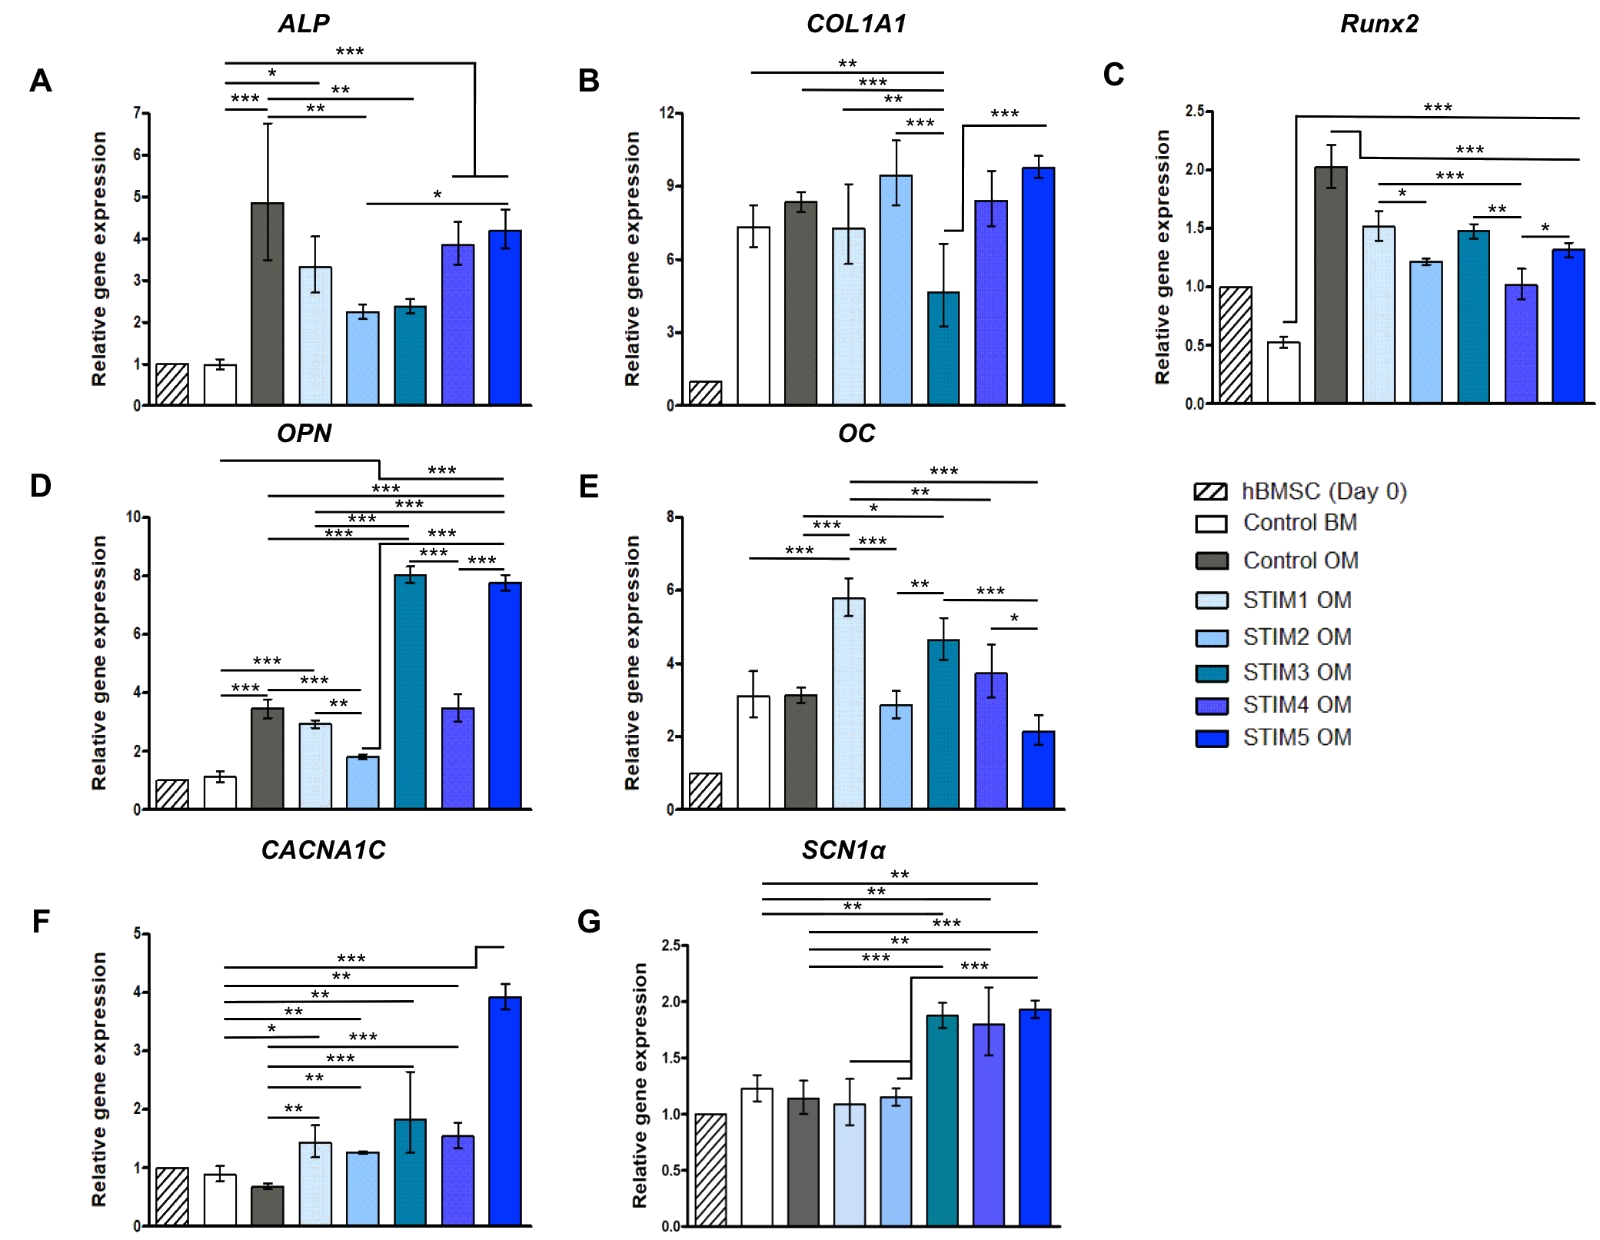
\includegraphics[scale=1.0]{./figures/Figure_4d10.png}}
\caption{Gene expression analysis by RT-qPCR of human bone marrow-derived \ac{MSCs} undergoing osteogenic differentiation under the different electric stimulation protocols for 14 days. Expressions of (A) ALP, (B) COL1A1, (C) Runx2, (D) OPN, (E) OC, (F) CACNA1C, and (G) SCN1$\alpha$ were normalized to the endogenous control GAPDH and calculated as a fold-change relative to the baseline expression of the control sample (hBM-MSCs at day 0). Results are expressed as average $\pm$ SD of three ($n=3$) independent samples. $*p < 0.05; **p < 0.01; ***p < 0.001$.}
\label{fig4d10}
\end{figure}

Immunofluorescence staining of the samples obtained after the osteogenic differentiation of human bone marrow-derived \ac{MSCs} exposed to the five different electric stimulation protocols was performed to assess the presence of the relevant bone \ac{ECM} proteins type I collagen, osteopontin, and osteocalcin. As shown in Figure \ref{fig4d11}, all three proteins (Col I, OPN, OC) were positively identified in all the experimental groups cultured under osteogenic induction conductions, with no noticeable differences in marker intensity expression being observed between the different electric stimulation protocols.

\begin{sidewaysfigure}
\makebox[\textwidth][c]{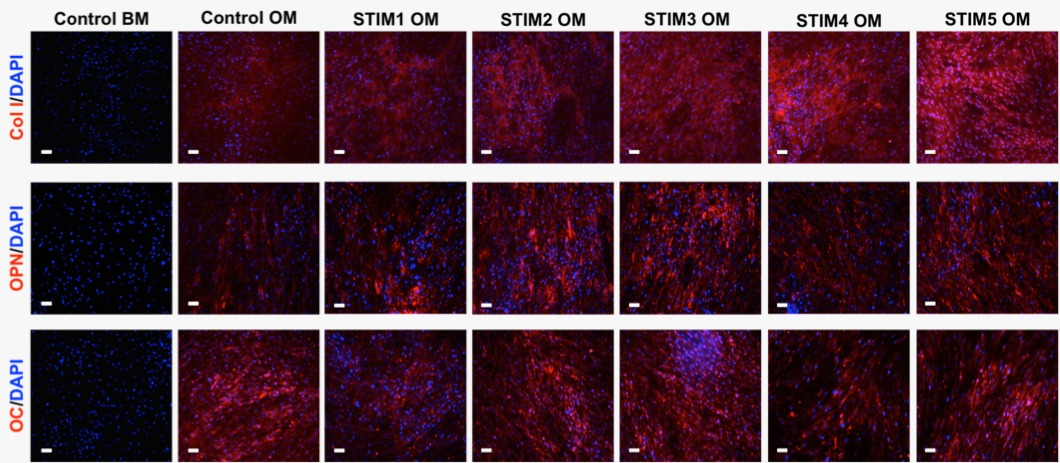
\includegraphics[scale=0.50]{./figures/Figure_4d11.jpg}}
\caption{Immunofluorescence analysis to evaluate the presence of type I collagen (Col I, top), osteopontin (OPN, middle), and osteocalcin (OC, bottom) bone-specific proteins on differentiating human bone marrow-derived \ac{MSCs} cultured under osteogenic induction conditions and exposed to the different electric stimulation protocols for 14 days (and respective non-stimulated controls). Antibody fluorescent staining in the samples appears in red. The samples were counterstained with DAPI, which stains cell nuclei in blue. Scale bar: 100 \si{\micro\meter}.}
\label{fig4d11}
\end{sidewaysfigure}


\section{Discussion}

\subsection{DCoupled setup response characterization and modelling}
An essential difference between direct-coupled systems using electrode/electrolyte interfaces (the system used in this work) and those that use agar salt bridges \cite{Song2007-qr} is that in the latter, only potassium and chloride ions flow from the agar salt bridge into the cell culture region. By contrast, when using immersed electrodes, uncontrolled and unknown free-flowing ions balance the charges by becoming oxidized and reduced in the process, which can unleash unexpected biological effects \cite{Srirussamee2019-ai, Srirussamee2021-cj}. The electrode may also release ions from its material, generating free radicals or being biologically active without further reactions. Stainless steel electrodes can not be considered inert, since they have been previously reported to release ferrous ions when subjected to pulsed stimulation. The ferrous ions release was strongly correlated with waveform parameters and the medium's ionic strength \cite{Tomov2000-db}. Despite this fact, this effect was neglected in the current study because the application of small constant electric currents or low-frequency potential waveforms is expected to release small ionic content into the media. This study unveils the predominant faradaic nature of the electrode/electrolyte interface between the stainless steel 316LVM and the BM or OM, which was established by applying a simple characterization process described by Biesheuvel \textit{et al.} \cite{Biesheuvel2018-wu}. Since our observations result from applying electric potentials inferior to the water hydrolysis limit, we can infer that other cell culture medium chemical species are being oxidized/reduced. This reinforces the importance of further understanding the faradic by-products that are being produced in \ac{DCoupled} stimulations when the electrode material is in direct contact with the culture medium, a necessity also highlighted by \cite{Srirussamee2019-ai, Tomov2000-db}. The average \acs{EF}s generated by our \ac{DCoupled} setup are predicted to be between 1.48 and 0.26 \si{\volt\per\meter}, corresponding to the time-dependent system responses to the input potential step signal, generating a peak electric current (0.17 \si{\milli\ampere}) that immediately drops to a much lower current (0.02-0.03 \si{\milli\ampere}). This peak effect is only observable when applying an electric potential step, since when applying an electric current step, the current source will adjust the electric potential of the electrode terminals in a time-dependent manner. Once the culture medium becomes more/less resistive, the current source will increase/decrease the electric potential at the electrode terminals to maintain the established current. The original \ac{DCoupled} setup from Mobini \textit{et al.} \cite{Mobini2016-jh} was subjected to a current measurement validation in a later work by Srirussamee \textit{et al.} \cite{Srirussamee2019-ai}. When they applied Mobini’s potential of 2.2 \si{\volt} DC, a total current of 0.07 $\pm$ 0.01 \si{\milli\ampere} (mean $\pm$ SD) was measured in each well after it reached a steady state. This measurement corresponds to the dwell phase of the system signal response, as we have observed here. Despite being of identical magnitude to our measured current at the same signal phase (0.02-0.03 \si{\milli\ampere}), the observed difference may arise from the differences in the electrical conductivity of the used culture medium and on the electrode material, which in turn generates a different electrode/electrolyte I-V curve interface relation, as shown in Figure \ref{fig4d5}.   

Since our developed DCoupled setup tries to emulate Mobini's \ac{DCoupled} setup, we also numerically modeled Mobini \textit{et al.} setup \cite{Mobini2016-jh} using the same methodology, considering their reported geometry and the posterior measured electric current by Srirussamee \textit{et al.}. We also took advantage of known typical electrical material properties for titanium, polystyrene, and culture medium. The average predicted \acs{EF} in Mobini's setup is 0.59 \si{\volt\per\meter} for the culture medium volume. This predicted electric field is lower than the reported by Mobini \textit{et al.} \cite{Mobini2016-jh} original setup and by other subsequent studies using the same setup \cite{Mobini2017-wp, Mobini2017-zr, Leppik2018-bw}, which report that a potential step of 2.2 \si{\volt} DC generated 100 \si{\volt\per\meter}. This value is contradicted by Srirussamee \textit{et al.} current measures (2019) \cite{Srirussamee2019-ai}, later repeated with more detail \cite{Srirussamee2021-cj} and with an additional potential measure at two distant points (8 \si{\milli\meter} apart) in the culture medium.

From Figure 2 in Srirussamee \textit{et al.} \cite{Srirussamee2021-cj} and with the help of a digitizer, the voltage drop between those two points can be estimated to be 0.0169 \si{\volt} (A: 0.8125 \si{\volt}, B: 0.7956 \si{\volt}). This potential measurement allows us to grossly estimate the \acs{EF} to be 2.1 \si{\volt\per\meter}, a magnitude value closer to our estimate. The difference between this value and the ones presented in our study may rely on the unknowns of the exact properties of the culture medium and the exact geometry of the electrodes and liquid volume used. Nevertheless, the measurements from Srirussamee \textit{et al.} \cite{Srirussamee2019-ai} and Tomov \textit{et al.} \cite{Tomov2000-db} reinforce the confidence in our delivered \ac{EF} prediction methodology. Also, the study from Zimmermann \textit{et al.} \cite{Zimmermann2021-fx}, describing the application of digital models to monitor and control electrical stimulation \textit{in vitro}, considered a stimulation chamber similar to the Mobini \textit{et al.} setup \cite{Mobini2016-jh}. Results from their \ac{DCoupled} model for Mobini’s DC stimulation conditions predicted an \ac{EF} of 0.33 \si{\volt\per\meter}, following Srirussamee \textit{et al.} \cite{Srirussamee2021-cj} current density predictions (0.5 \si{\ampere\per\square\meter}). That prediction agrees with our model calculations for Mobini’s \ac{EF} magnitude (0.59 \si{\volt\per\meter}), differing from the values of 100 \si{\volt\per\meter} reported by Mobini \textit{et al.}. Regarding \ac{DCoupled} stimulation regimes using directly immersed electrodes, agar-salt bridges, or a conductive scaffold substrate, a mandatory reading for further understanding of the electrochemistry effects in each setup is the theoretical analysis of Guette-Marquet \textit{et al.} \cite{Guette-Marquet2021-rp}. Their analysis also suggests that, for two-electrode systems (like the one used here), many reported \ac{EF} magnitude values have been overestimated, which is also in line with Zimmermann \textit{et al.} \cite{Zimmermann2021-fx} and our predictions. Guette-Marquet \textit{et al.} also advises changing experimental practices by applying current instead of voltage, a condition that we implemented in the protocol condition STIM3 OM. We monitored and reported the resultant electric current for the remaining potential conditions. Although we have used a direct probing method (multimeter) to measure the electric current that passes through the system, indirect probing methods should be privileged in the future to avoid direct influence in effects, like the Rogowski-coil method of measuring electric current \cite{Ward1993-wl}.


\subsection{Effects of different electric stimulation protocols on \ac{MSCs} osteogenic differentiation}
The successful clinical outcomes of electric stimulation in bone healing strategies encouraged the scientific community to try to understand its underlying mechanisms at the cellular and molecular levels. Electric stimulation has been previously applied to enhance the osteogenic differentiation of \ac{MSCs} \textit{in vitro} \cite{Guillot-Ferriols2022-wn, Peng2023-ud, Bianconi2023-rs}. However, the cellular processes/signaling pathways by which electric stimulation regulates osteogenesis are still poorly understood. Therefore, there is no optimal, defined, standardized electric stimulation protocol for inducing \ac{MSCs} osteogenic commitment \textit{in vitro}. Many studies using poorly characterized experimental systems for electric stimulation limit the comparison of results and protocol reproducibility. Existing studies often use single voltage-controlled protocols to treat \ac{MSCs} without using numerical modelling to visualize the output of the selected stimulation parameters. They usually analyze the results only by comparing them to non-stimulated controls, unable to compare their results with other existent works. Moreover, current-based electric stimulation protocols imposing current intensity instead of voltage is vastly unexplored \cite{Guette-Marquet2021-rp}.

Thus, in this study, we aimed to directly compare different potential-controlled electric stimulation protocols with a current-controlled one in terms of their capacity to improve the in vitro osteogenesis of human bone marrow-derived \ac{MSCs}. The \ac{EF} magnitude calculation performed will allow us to compare this work output with similar future studies. All the electric stimulation protocols resulted in final cell cultures with high viability, high metabolic activity, and regular cell morphology (Figure \ref{fig4d7}). These results follow the study from Zhao \textit{et al.} \cite{Zhao2011-wy}, which reported high cell viabilities (90-95\%) and typical elongated fibroblast-like morphology for human bone marrow-derived \ac{MSCs} exposed to \ac{EFs} of 200 \si{\milli\volt\per\milli\meter} (two orders of magnitude higher than the \ac{EFs} applied in this work). Regarding the applied current-controlled protocol (STIM3 OM), the overtime increase in metabolic activity (indirect measure of cell proliferation, AlamarBlue assay) observed in Figure \ref{fig4d7}A and high cell viability/regular cell morphology (Figure \ref{fig4d7}B) are concordant with the results reported by Shao \textit{et al.} \cite{Shao2011-dz} for osteoblasts exposed to DCoupled electric stimulation of 100 \si{\micro\ampere} (4 \si{\hour} per day) for six days.

The effects of the different electric stimulation protocols on the human bone marrow-derived \ac{MSCs} osteogenic differentiation were assessed after 14 days through the quantification of ALP activity and calcium production (Figure \ref{fig4d8}), typical osteogenic stainings (Figure \ref{fig4d9}), bone-related marker genes expression (Figure \ref{fig4d10}) and immunofluorescence analysis of essential bone ECM proteins (Figure \ref{fig4d11}). Our results suggested an advantageous performance of the applied current protocol (STIM3 OM) in enhancing calcium production/mineralization by osteogenic differentiating human bone marrow-derived \ac{MSCs} (Figure \ref{fig4d8}B). This result concurs with the more intense and spread Alizarin Red and Xylenol Orange stainings observed in Figure \ref{fig4d9} for the cultures exposed to STIM3 OM protocol. Moreover, the higher mineralization observed for the applied current electric stimulation condition is supported by the previous study performed by Zhang \textit{et al.} \cite{Zhang2016-ul}, in which significantly higher calcium deposition was obtained (at day 14) for human adipose-derived \ac{MSCs} cultured on polypyrrole/polycaprolactone scaffolds under osteogenic induction and exposed to 200 \si{\micro\ampere} of direct current for 4 \si{\hour} per day.

All the electric stimulation protocols resulted in similar or lower ALP activities (Figure \ref{fig4d8}A) and \textit{ALP} (Figure \ref{fig4d10}A), \textit{Runx2} (Figure \ref{fig4d10}C) gene expressions than the non-stimulated Control OM group. Such observation might be explained by the fact that \textit{Runx2} and \textit{ALP} expressions (and respective ALP activity) are more predominant in the initial phase of MSC’s osteogenic differentiation (early markers) that precede the mineralization phase, after which their levels decrease \cite{Beck2003-fx}. Thus, it is possible that electric stimulation protocols promoted a faster osteogenic differentiation (as supported by the enhanced mineralization (Alizarin Red staining, Figure \ref{fig4d9}), upregulation of late-stage markers (\textit{OPN} (Figure \ref{fig4d10}D) and \textit{OC} (Figure \ref{fig4d10}E)) expression and respective proteins presence in Figure \ref{fig4d11}), resulting in the observed lower \textit{Runx2} and \textit{ALP} expressions.

OPN has been shown to play a pivotal role in regulating calcium phosphate nucleation during the mineralization process \cite{Liu2020-zx}. Thus, the significantly higher \textit{OPN} gene expression observed in Figure \ref{fig4d10}D for the cultures exposed to STIM3 OM protocol is well correlated with the enhanced mineralization obtained for the same condition (Figure \ref{fig4d8}B and Figure \ref{fig4d9} - Alizarin Red and Xylenol Orange stainings). This beneficial effect of applied current electric stimulation on \textit{OPN} expression and mineralization has been previously reported \cite{Zhang2016-ul}. \textit{OC} gene upregulated expression has also been associated with improved bone mineralization \cite{Zoch2016-bn}. Therefore, the significantly higher \textit{OC} expressions obtained for the experimental groups STIM1 OM and STIM3 OM might explain these conditions’ improved calcium production (Figure \ref{fig4d8}B) and more intense mineral deposition (Alizarin Red staining, Figure \ref{fig4d9}).

\textit{CACNA1C} gene role in the signaling cascade regulating the osteogenic differentiation of human MSCs and subsequent tissue mineralization has been demonstrated in previous works \cite{Zhang2016-ul}. Zhang \textit{et al.} showed the superior role of voltage-gated calcium channels in the modulation of adipose-derived \ac{MSCs} in comparison to other ionic channels (sodium, potassium, and chloride) \cite{Zhang2016-ul}. Moreover, the study from Camarero-Espinoza and Moroni further evidenced the correlation between \textit{CACNA1C} and the osteogenic differentiation of human bone marrow-derived \ac{MSCs}, as they showed that blocking the activity of \textit{CACNA1C} resulted in a downregulation of the bone-specific genes (\textit{Runx2}, \textit{COL1A1} and \textit{OC}) \cite{Camarero-Espinosa2021-dh}. Previous studies have proposed that electric stimulation promoted the increase of cytosolic calcium ionic concentration both in osteoblasts and \ac{MSCs}, which subsequently activates voltage-gated calcium channels and regulates cell functions via calmodulin pathways \cite{Zhang2016-ul, Zayzafoon2006-vc}. Accordingly, our results showed that all the electric stimulation protocols resulted in the upregulation of \textit{CACNA1C} expression (Figure \ref{fig4d10}F) with the highest levels observed for the STIM5 OM condition. STIM5 OM protocol also promoted the highest \textit{COL1A1} expression (Figure \ref{fig4d10}B), which is in line with the relation between \textit{CACNA1C} and \textit{COL1A1} genes previously suggested in the study from Camarero-Espinoza and Moroni \cite{Camarero-Espinosa2021-dh}.

The different electric stimulation protocols employed resulted in distinct cellular responses, particularly regarding \ac{MSCs} gene expression profiles (Figure \ref{fig4d10}). Considering the protocols STIM1 OM (1 hour, Higher \ac{EF}+Lower \ac{EF}) and STIM2 OM (1 second, Higher \ac{EF}), it appears that a single pulse of high \ac{EF} (STIM2 OM) is sufficient to achieve \textit{ALP}, \textit{COL1A1}, \textit{CACNA1C} and \textit{SCN1$\alpha$} expressions similar to STIM1 OM. However, a more prolonged stimulation (prevalence of the Lower \ac{EF} signal component) seems to be advantageous for higher expressions of more mature marker genes (\textit{OPN} and \textit{OC}) and mineralization (intense and spread Alizarin Red staining, Figure \ref{fig4d9}), suggesting a more advanced differentiation stage achieved by the cells exposed to STIM1 OM than STIM2 OM. This effect is also observed comparing a single pulse of high \ac{EF} (STIM2 OM) with multiple pulse protocols (STIM4 OM and STIM5 OM), in which the latter resulted in higher levels of bone-specific gene expression. Statistical significant differences in gene expression levels (\textit{Runx2}, \textit{OPN}, \textit{OC} and \textit{CANA1C}) were also observed between the protocols STIM4 OM (1 hour, sequence of multiple Higher \ac{EF} + short duration Lower \ac{EF}) and STIM5 OM (1h, sequence of multiple Higher \ac{EF} + short duration Lower \ac{EF}, with five times more pulses than STIM4 OM), suggesting the relevance of the signal period/frequency in the modulation of \ac{MSCs} osteogenic differentiation. Concordantly, Wang \textit{et al.} \cite{Wang2016-ff} study showed that different frequencies of electric stimulation lead to distinct outcomes in the \textit{in vitro} osteogenesis of MC3T3-E1 pre-osteoblastic cells.

In general, our results (higher mineralization and \textit{OPN} gene expression) suggest the benefits of using a current-controlled electric stimulation protocol (STIM OM3) for the in vitro stimulation of \ac{MSCs} towards the bone lineage. We are aware that this improved performance in STIM3 OM may result from the potential signal oscillation at the electrodes that, when trying to support the prescribed current, increased the potential above 1.2 \si{\volt}, which probably generated uncontrolled and unknown redox artifacts that might influence \ac{MSCs} response. Previous studies have reported the role of reactive oxygen products on the enhancement of MSC osteogenic differentiation \cite{Srirussamee2021-cj, Sheppard2022-gj}. Despite this limitation, our work provides valuable insights towards the \textit{in silico} and \textit{in vitro} optimization of electric stimulation protocols for producing high-quality clinically relevant \ac{MSCs}-based \ac{BTE} products for bone repair treatments.

Future work will include further optimization of the applied current-controlled electric stimulation protocols toward improved osteogenesis combined with whole transcriptome analysis. This will allow the unraveling and understanding of underlying molecular mechanisms/signaling pathways by which current-controlled electric stimulation modulates \ac{MSCs} osteogenesis. Those electric stimulation protocols could also be applied to basal medium cultures to find if an electric stimulus on its own could replace the addition of osteogenic promoters. Developing new scalable devices for electric stimulation to allow a middle/high-throughput analysis will also be considered.


\section{Summary}

This chapter points out that the custom-developed \acs{DCoupled} system will generate redox reactions in the electrode/electrolyte interface even for potential differences inferior to the water electrolysis limit, observable by the characteristic system's electric wave response. So, once unknown chemical species present in the medium solution are oxidized or reduced, \acs{DCoupled} systems like this one may generate uncontrollable and unpredictable cellular interactions, which, in turn, will hamper the conclusions regarding the effects of the applied \acs{EF}. 

A numerical \acs{FEM} digital model of the cell culture condition and \acs{DCoupled} system was employed to characterize and predict the magnitude distribution of the electric fields generated by the different stimulation protocols. The models successfully assessed the impact of small culture medium volume and electrode geometrical variations on the delivered \acs{EF}. Performed \textit{in vitro} cell culture studies showed that all the electric stimulation protocols applied did not cause any impairment in cell viability and morphology, effectively supporting the osteogenic differentiation of human bone marrow-derived \ac{MSCs}. Differences observed in the provoked cellular effects between all the applied protocols conclude that osteogenic gene expression was promoted in all protocols when compared to osteogenic media control regarding the expression of COL1A1, CACNA1C, SCN1$\alpha$. Applying just a single higher \acs{EF} signal phase does not affect ALP activity and calcium content. However, increasing the number of times this signal was applied increased the gene expression of APL, Osteopontin, CACNA1C, and SCN1$\alpha$ correspondingly. Moreover, it is important to notice that applying different stimulation protocol parameters has been shown to promote different gene expression conditions.  

Despite the practical nature of \acs{DCoupled} setups and their capabilities as a tool to promote osteogenesis, this thesis moved on to a more reliable capacitive coupled stimulation system that guarantees stimulation without electron transfer processes. Thus bypassing the unresolved faradaic uncertainties associated with \acs{DCoupled} systems that were observed in this chapter.


%\newpage
%\bibliography{library_c4b} 
%\bibliographystyle{plain}
%\end{document}
%\documentclass[11pt]{report}
%\usepackage{siunitx}
%\usepackage{graphicx}
%\usepackage{multirow}
%\usepackage[table,xcdraw]{xcolor}
%\usepackage{amsmath}
%\usepackage{longtable}
%
%\begin{document}
%\setcounter{chapter}{4}
%\tableofcontents



\newpage
\chapter{Numerical modelling of capacitive-coupled stimulation}
This chapter contains the results of the numerical modelling approaches applied to capacitive-coupled setups to predict the generated electric field. This chapter describes the work presented in the following published works:
\begin{itemize}
\item \small \textit{Meneses, Joao, Sofia R. Fernandes, Nuno Alves, Paula Pascoal-Faria, and Pedro Cavaleiro Miranda. 2021. “Effects of Scaffold Electrical Properties on Electric Field Delivery in Bioreactors.” Conference Proceedings: Annual International Conference of the IEEE Engineering in Medicine and Biology Society. IEEE Engineering in Medicine and Biology Society. Conference 2021 (November): 4147–51.};
\item \small \textit{Meneses, João, Sofia Fernandes, Nuno Alves, Paula Pascoal-Faria, and Pedro Cavaleiro Miranda. 2022. “How to Correctly Estimate the Electric Field in Capacitively Coupled Systems for Tissue Engineering: A Comparative Study.”, Scientific Reports 12 (1): 12522.};
\end{itemize}


\newpage
\section{Introduction}

As defined in Chapter 1, \acs{CCoupled} setups are composed of two electrodes physically separated from the cell culture medium through an electric insulator material, usually an air gap or a petri dish wall. This electric insulator layer obstructs any electron transfer reactions, so the electric signal propagation to the cell culture medium is only possible through a time-varying electric displacement field. This displacement field polarizes the insulator material layers and the cell culture medium trapped between them. In the insulator, the polarization mechanism involves aligning electric dipoles with the applied \acs{EF} (complete absence of free charges). On the other hand, in the culture medium, polarization occurs due to the flow of (free) charged particles, usually ions. The resultant polarization will originate an \acs{EF} in the dielectric medium (insulator layers plus cell culture medium) that opposes the direction of the initially applied \acs{EF} \cite{Ida_undated-cu}. 

Accurate estimates of the \acs{EF} applied by CCoupled setups are essential to compare results from different studies and establish a relation between stimulus characteristics and specific cellular effects. However, this quantity is rarely measured and often estimated with incorrect assumptions of the underlying physics. This chapter includes two works performed on modelling \acs{CCoupled} setups to help understand which factors most affect the generated \acs{EF} delivery for this particular stimulation setup.   

The first work investigated the influence of scaffolds on the \acs{EF} delivered inside a bioreactor \acs{CCoupled} setup, since it constitutes an effect often neglected. Multiple electrical conductive and non-conductive biomaterials have been developed for \acs{BTE} cell culture substrates in a variety of forms (porous scaffolds, films, nanofibers, coatings) \cite{Dong2020}. After cell seeding, this structure is subjected to an electrical stimulation employing, for example, \acs{CCoupled} setups to achieve the desired cell function modulation. The ubiquitous use in the literature of cell support materials in experimental protocols applying electrical stimulation should be addressed in terms of their impact in the \acs{EF} at cellular targets. This impact should then be considered when selecting the scaffold geometry and/or material, in order to ensure no interference or even synergy with the induced \acs{EF}. In this work, we considered the \acs{CCoupled} setup based on Brighton's original work \cite{Brighton1988-vc, Brighton1992-gg} to analyze the impact of a scaffold insertion in the \acs{EF} characteristics. A geometrical model for this setup was created, and a sensitivity analysis was performed using the \acs{FEM}. After validating our model with the experimental measures made by Brighton \textit{et al.} \cite{Brighton1988-vc, Brighton1992-gg} in an empty chamber, an orthogonal scaffold was introduced in the culture medium, and an extensive sensitivity analysis of the delivered \acs{EF} was performed for different values of function of the electrical conductivity and permittivity of the scaffold material and culture medium. Understanding the influence of scaffold geometry and material composition in the delivery of \acs{CCoupled} \acs{EF}s will allow the building of precise, reliable, and replicable stimulation protocols.   

The second work reported in this chapter applies modelling methods to \acs{CCoupled} systems reported in previous literature to corroborate estimates of the \acs{EF} in the culture medium. For this purpose, eight \acs{CCoupled} studies were analyzed as shown in Figure \ref{fig5d1}. The fundamental physics underlying \acs{CCoupled} stimulation were reviewed, and then, three modelling approaches were delineated to estimate the \acs{EF}: two of them based on solving an analog electric circuit model, the first by solving analytically the circuit to find the electric current in the culture medium and the produced \acs{EF}, the second by performing the same steps using LTSpice as a solver, an analog electronic circuit simulator computer software (allowing more complex waveform solutions); the third and last approach was to apply the \acs{FEM} to model the \acs{CCoupled} system geometry and solve it with a golden standard software. A free, open-source tool was developed to perform the models using the first approach and ease future calculation of the \acs{EF} being delivered by \acs{CCoupled} systems in \acs{TE} and \acs{BTE} applications. This \acs{EF} Calculator for \acs{CCoupled} systems is available for download from Zenodo hosting platform \cite{Meneses2022-yk}. An extremely large span of \acs{EF} strengths in the culture medium has been reported for \acs{CCoupled} setups alone, ranging from \num{1.0d-5} \si{\volt\per\meter} \cite{Fitzsimmons1986-ks} to \num{1.7d5} \si{\volt\per\meter} \cite{Rodan1978-yu}. In these studies, different methods were used to estimate the \acs{EF} strength, some of them flawed. Yet, they all describe a positive effect of electrical stimulation on cell culture, and some of them are widely cited. This work aims to determine the validity of the \acs{EF} strength estimated in several \acs{CCoupled} \textit{in vitro} studies by comparing it with the predictions from three different modelling approaches. This work also presents a solid theoretical and practical methodology to estimate the \acs{EF} in \acs{CCoupled} stimulation protocols, thus contributing to enhance reproducibility and help to establish guidelines when \acs{CCoupled} systems are used in \acs{BTE} applications.

\begin{figure}[h]
\makebox[\textwidth][c]{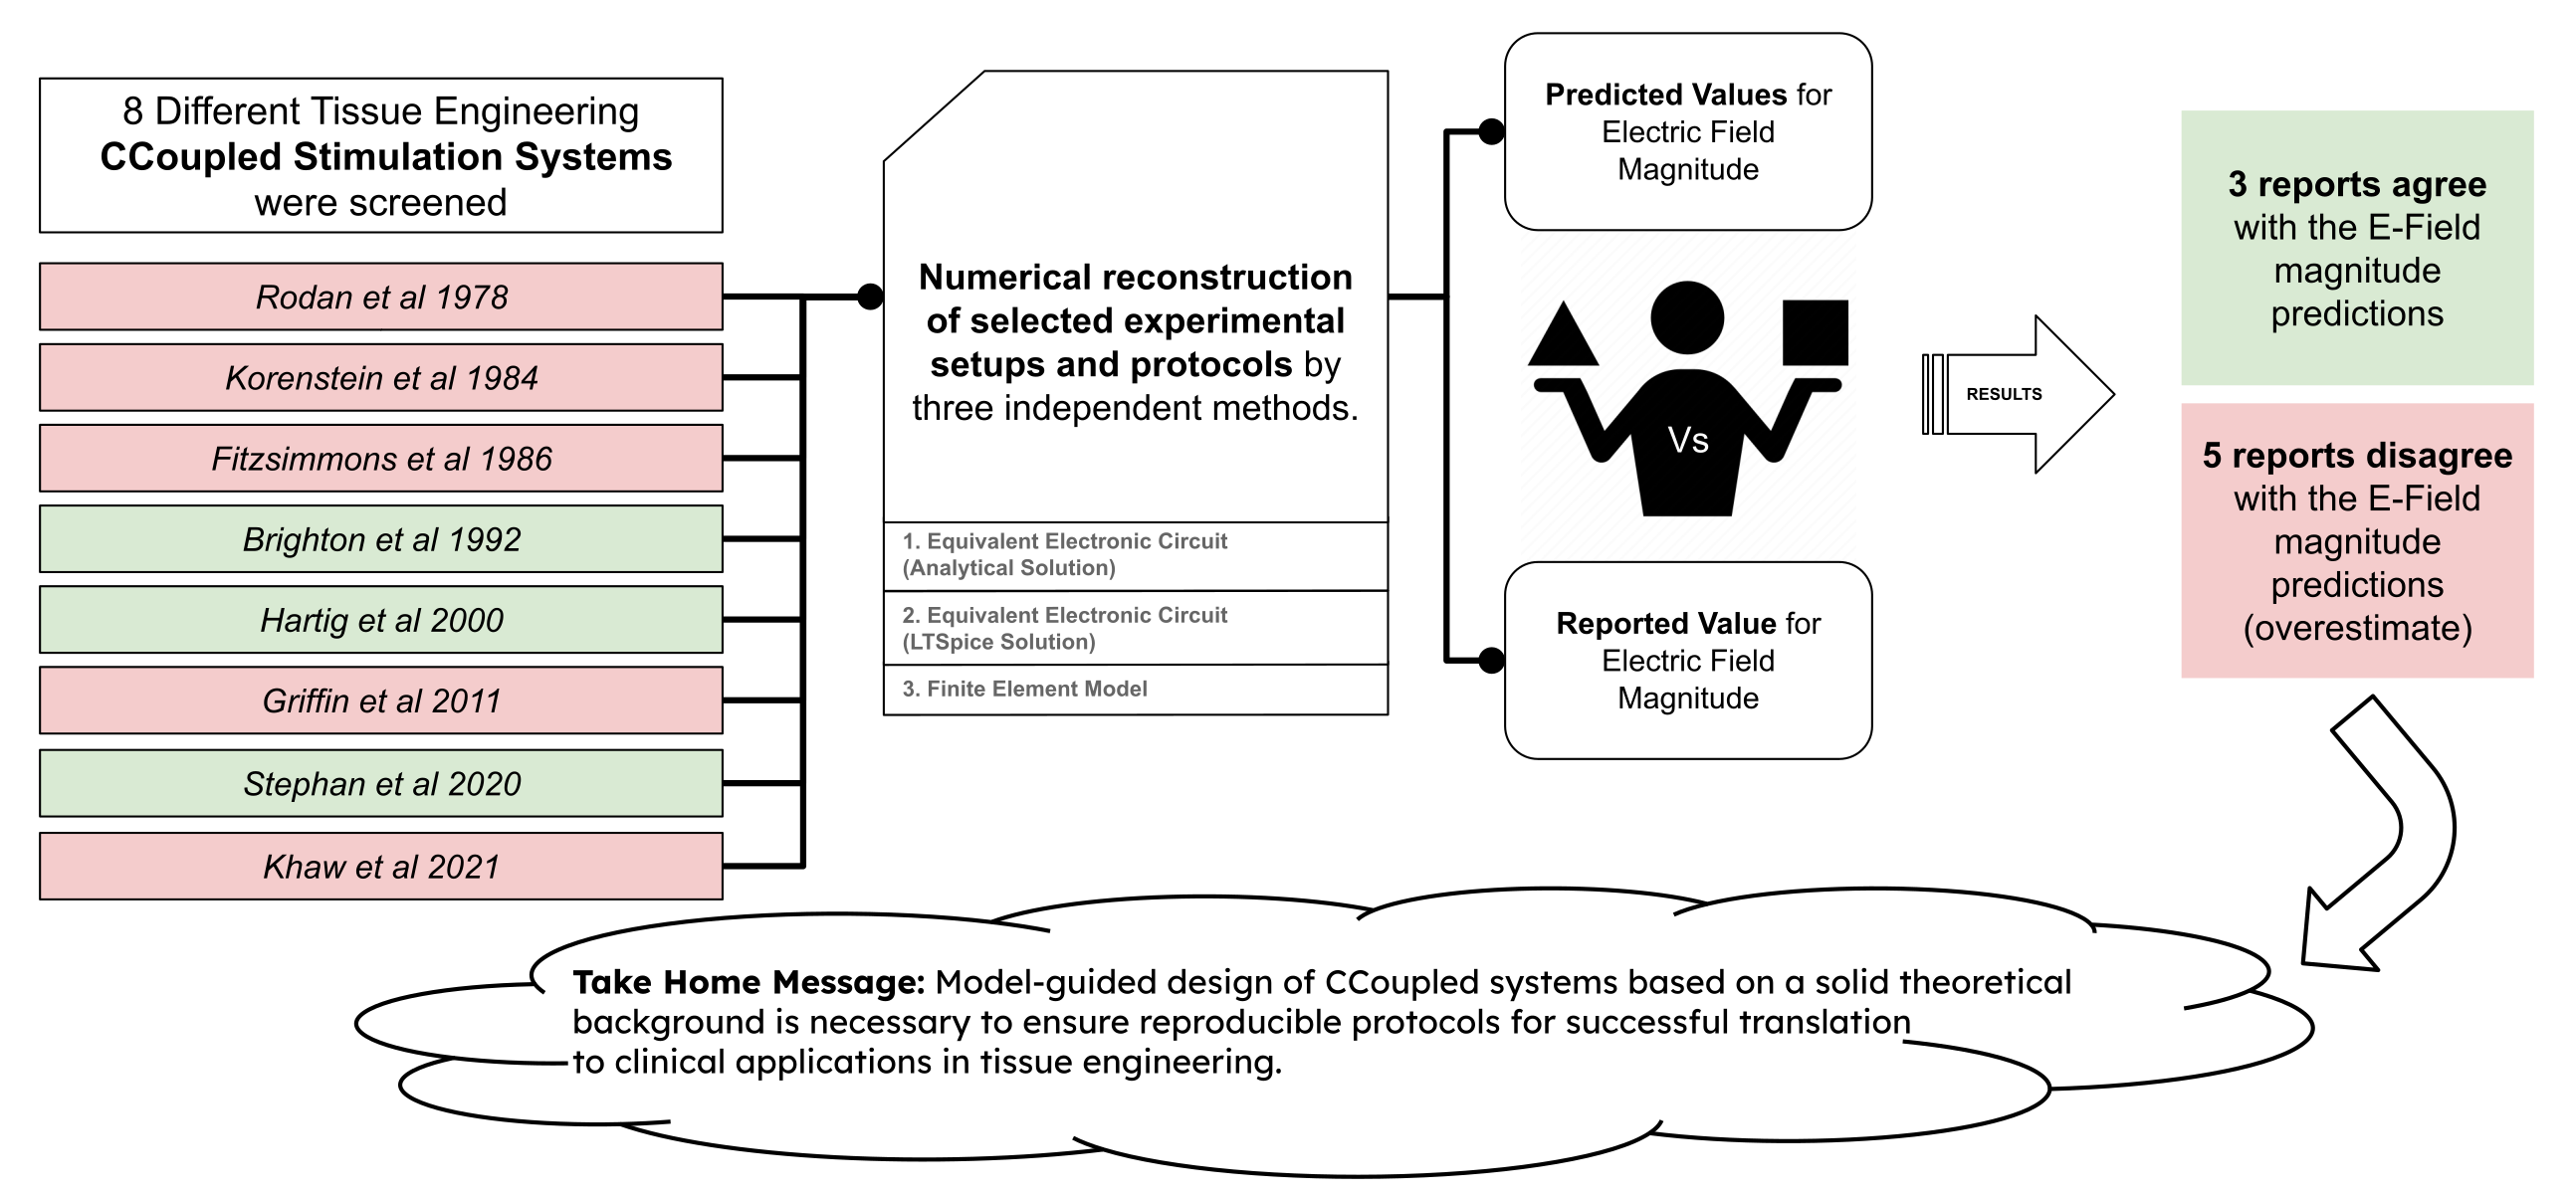
\includegraphics[scale=0.55]{./figures/Figure_5d1.png}}
\caption{Graphical abstract for the work of modelling published CCoupled setups in \acs{BTE}.}
\label{fig5d1}
\end{figure}




\section{Aim}
\begin{itemize}
\item To model the effects of adding scaffold structures into the empty cell culture chamber (containing just culture medium) of an existent \acs{CCoupled} setup;
\item To model the \acs{EF} that is delivered by several reported \acs{CCoupled} setups and protocols, comparing their predictions with the values obtained from the literature;
\end{itemize}




\section{Methods}




\subsection{Scaffold insertion effects}

\textit{Brighton \acs{FEM} Model - Cell Culture Chamber Without Scaffold.} The \acs{3D} model replicating Brighton's experimental setup, as described in \cite{Brighton1988-vc, Brighton1992-gg}, was constructed using SOLIDWORKS software (version 2018, Dassault Systemes SolidWorks Corporation, France). The geometry is composed of 5 co-axial cylindrical domains with a diameter of 33 \si{\milli\meter} (see Figure \ref{fig5d2}A): two stainless steel electrodes, with a thickness of 1 \si{\milli\meter}; two glass coverslips placed between the electrodes and the culture medium, with a thickness of 0.16 \si{\milli\meter}; one cell culture medium chamber that occupies the entire central region, with a thickness of 10 \si{\milli\meter}. The dimensions not specified in Brighton's setup descriptions were estimated based on the drawing from its 1992 manuscript \cite{Brighton1992-gg} and similar commercially available parts. \hfill \break


\begin{figure}
\makebox[\textwidth][c]{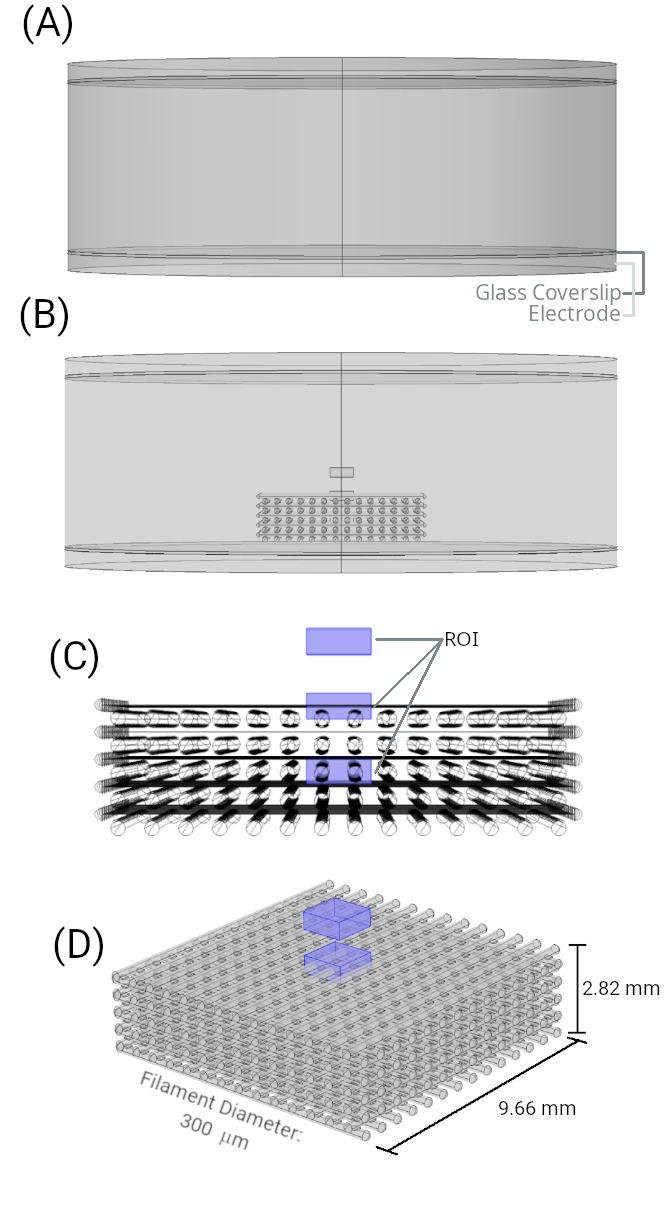
\includegraphics[scale=1.0]{./figures/Figure_5d2.png}}
\caption{Model geometry. (A) \acs{3D} model of Brighton's experimental setup, composed of 5 distinct domains: two electrodes (top and bottom); two glass coverslips (top and bottom); and one culture medium domain (central). (B) A \acs{3D} model with orthogonal scaffold placed at the bottom of the cell culture medium chamber. (C) Three equidistant and equal-sized rectangular prism \acs{ROI}s (tinted blue) represent the scaffold environment's external, interface, and internal regions. (D) Volumetric view of the orthogonal scaffold with overall dimensions and the \acs{ROI}s (tinted blue).}
\label{fig5d2}
\end{figure}


\noindent \textit{Brighton \acs{FEM} Model - Cell Culture Chamber With Scaffold.} To the previously described \acs{3D} model, an orthogonal scaffold was added at the bottom of the cell culture medium chamber (see Figure \ref{fig5d2}B). This scaffold comprises alternating horizontal layers of 300 \si{\micro\meter} filaments, whose centers are 600 \si{\micro\meter} apart. Consecutive layers are rotated by 90\si{\degree}. To avoid meshing and numerical problems associated with point contacts and sharp edges, the tips of each filament were rounded, and an overlap of 20 \si{\micro\meter} was introduced between adjacent horizontal layers, which are then separated by 580 \si{\micro\meter}. For the same reason, the bottom of the scaffold is placed 350 \si{\micro\meter}  above the bottom of the chamber. Three equidistant and equal-sized rectangular prism \acs{ROI}s were added to the 3D model to allow detailed studies in these regions (see Figure \ref{fig5d2}C, \ref{fig5d2}D). \hfill \break

\noindent \textit{Numerical Model Parameters.} \acs{FEM} analysis was conducted with the AC/DC module of COMSOL Multiphysics (version 5.2a, Stockholm, Sweden). The Electric Current (ec) physics interface was selected, considering a frequency-domain study at 60 \si{\kilo\hertz}. A \acs{3D} physics-controlled mesh was also generated in COMSOL for each model (with and without scaffold), considering the finer mesh option. Both models are composed of three common materials: stainless steel for electrodes ($\sigma$: \num{4.032d6} \si{\siemens\per\meter}, $\epsilon_r$: 1.0); cover glass N1 insulating walls ($\sigma$: \num{1.0d-13} \si{\siemens\per\meter}, $\epsilon_r$: 6.85); and cell culture medium. The model with scaffold also contains the scaffold material, the properties of which were varied in a parametric sweep study together with the culture medium properties (Table \ref{table_sensitivity}). Following Brighton's work \cite{Brighton1988-vc, Brighton1992-gg}, an electric potential boundary condition of 44.81 \si{\volt} was added to the top surface of the top electrode, and a ground boundary condition was added to the bottom surface of the bottom electrode. COMSOL \acs{BiCGStab} stationary iterative solver was used to run this parametric sweep study, due to its ability to handle a wide range of matrices (memory efficiency), often converging faster than other iterative solvers. \hfill \break



\begin{table}
\caption{Sensitivity Analysis Study Parameters. Selected parameters match common scaffold materials and culture medium properties.}
\bigskip
\scriptsize
\centering
\begin{tabularx}{350px}{l l l} \toprule[0.15em]
& \textbf{Culture Medium}  & \textbf{Scaffold}  \\ \cmidrule(l){1-3}
\textbf{Electrical Conductivity} $\sigma_{cm}$ (\si{\siemens\per\meter}) & \textit{1.1, 1.5, 1.9} & \textit{\num{1.0d-14}, 0.001, 0.005, 0.01, 0.05,} \\
& & \textit{0.1, 0.5, 1.1, 1.3, 1.5, 1.7, 1.9, 10, 50,} \\
& & \textit{100, 150, 300, 500, 1000, \num{7.5d5}} \\
\textbf{Relative Permittivity} $\epsilon_{cm}$ (dimensionless) & \textit{50, 80.1, 90} & \textit{1, 2.2, 80.1} \\ \bottomrule[0.15em]
\end{tabularx}
\label{table_sensitivity}
\end{table}


\noindent \textit{Sensitivity and Spatial Distribution Analysis.} Sensitivity analysis was performed employing a one-at-a-time variation method, applied to the results obtained from the COMSOL parametric sweep study. This parametric sweep study generated 540 different solutions, one for each combination of the input parameters described in Table \ref{table_sensitivity}, with electrical conductivities and permittivities values obtained from \cite{Gavish2016-av, Bennett2019-js, Mazzoleni1986-wp}. \acs{EF} data were then exported from COMSOL Multiphysics software to text file format for further postprocessing in custom-made Python scripts (using Pandas, Matplotlib, and SALib libraries). These Python scripts were used to generate the plots and histograms for sensitivity and spatial distribution analysis. Sensitivity analysis was performed by the method of Delta Moment-Independent Measure, implemented in the python SALib library, according to the original works of Borgonovo \textit{et al.} and Plischke \textit{et al.} \cite{Borgonovo2007-tj, Plischke2013-ok}. Sensitivity and spatial distribution analysis were independently performed for each \acs{ROI} (external, interface, and internal), where only the culture medium nodes data were considered. Spatial distribution analysis was performed on three authentic scaffold materials from the \acs{TE} field (Thermoplastic \cite{Hegde2015-nd}, Hydrogel \cite{Distler2020-gi}, Metalic \cite{MetalInfo}), and also on a control scaffold with the same material electrical properties of the cell culture medium (no effect of scaffold presence is expected under this condition).


\subsection{Modelling \acs{CCoupled} reported setups}


\noindent \textit{Electric Circuit Model of \acs{CCoupled} Experimental Setups.} The geometry of experimental setups for \acs{CCoupled} electrical stimulation of cells can often be modeled as shown in the previous section by using a cylindrical layered geometry, with two circular metallic plates separated from the culture medium by electrically insulating layers, typically plastic, glass, or air, as shown schematically in Figure \ref{fig5d3}a. Note that all layers have the same diameter in this model. Given the setup's geometry, the electric charge flows parallel to the cylinder's axis.  In general, each layer can be described in terms of a resistor and a capacitor in parallel (Figure \ref{fig5d3}b) since both paths are available for the flow of charge.


\begin{figure}
\makebox[\textwidth][c]{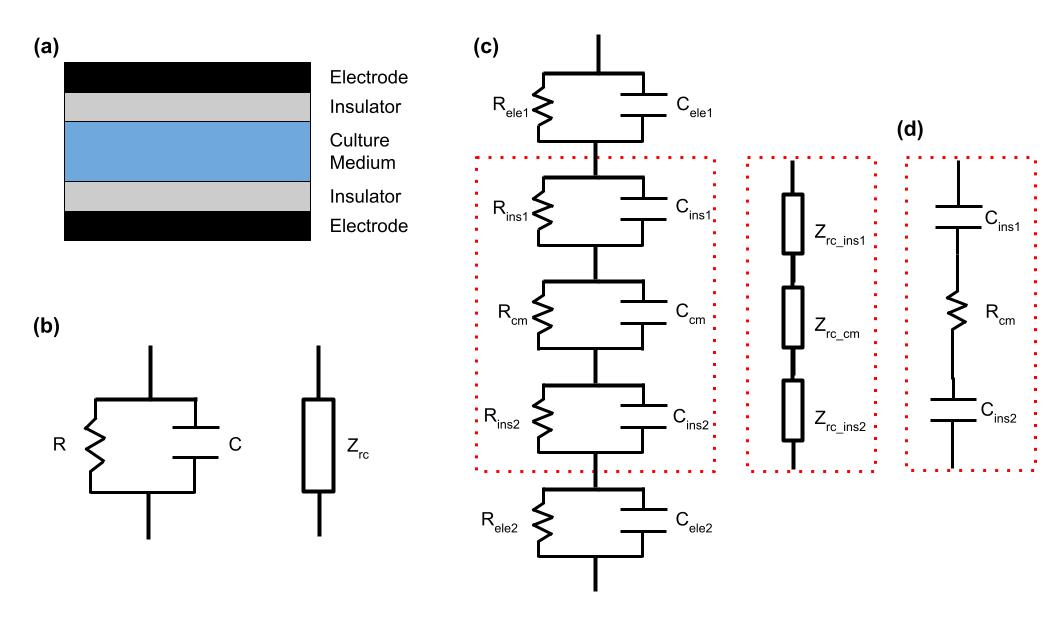
\includegraphics[scale=1.5]{./figures/Figure_5d3.png}}
\caption{(a) Layered cylindrical model of a typical \acs{CCoupled} experimental setup; (b) Resistor-capacitor (RC) model and impedance circuit model for an individual layer; (c) RC and impedance circuit models for the five layers; (d) The complete circuit can be reduced to its three most relevant components without significant loss of accuracy. Abbreviations: ele-electrode, ins-insulator, cm-culture medium, r-resistor, c-capacitor, z-impedance.}
\label{fig5d3}
\end{figure}

In this geometry, the \acs{EF} within each layer is uniform so the resistance, $R_i$, and capacitance, $C_i$, of the $i^{th}$ layer are given by the familiar formulae,

\begin{equation}
\label{eq2}
R_i = \rho_i \frac{l_i}{A}
\end{equation}

\begin{equation}
\label{eq3}
C_i = \frac{\epsilon_{0} \epsilon_{r_i} A}{l_i}
\end{equation}

\noindent where $\rho_i$ is the resistivity of the material, $\epsilon_{r_i}$ its relative permittivity and $\epsilon_{0}$ the permittivity of vacuum, $A$ is the cross-sectional area of the cylinder and $l_i$ the thickness of the layer. The relation between the current, $I$, which is the same in all layers due to charge conservation, and the voltage drop in each layer, $V$, is given by Ohm’s law

\begin{equation}
\label{eqOhms}
V_i = Z_i I
\end{equation}

\noindent where $Z_i$ is the impedance of the $i^{th}$ layer. Note that this is the impedance of the resistor, $Z_r$, and of the capacitor, $Z_c$, in parallel, i.e.,

\begin{equation}
\label{eqLayerimpedance}
\frac{1}{Z_{i}} = \frac{1}{Z_{r_i}} + \frac{1}{Z_{c_i}}
\end{equation}

The impedances of the resistor and capacitor are defined by:

\begin{equation}
\label{eqRimpedance}
Z_{r_i} = R_i
\end{equation}

\begin{equation}
\label{eqCimpedance}
Z_{c_i} = j X_{c_i} = -\frac{j}{\omega C_i}
\end{equation}

\noindent where $X_{c_i}$ is the capacitive reactance, $\omega$ is the angular frequency of the applied sinusoidal signal, and $j$ is the imaginary unit. Thus

\begin{equation}
\label{eqLayerimpedance2}
\frac{1}{Z_{i}} = \frac{1}{R_i} + j \omega C_i
\end{equation}

\noindent or

\begin{equation}
\label{eqLayerimpedance22}
Z_{i} = \frac{R_i (1 - j \omega C_i R_i)}{1 + \omega^{2} C_i^{2} R_i^{2}}
\end{equation}

\noindent Note that impedances are complex numbers and that the impedance of a capacitor is frequency dependent, it decreases with increasing frequency. 

The whole setup can be viewed as a series of five parallel RC circuits, one for each layer (Figure \ref{fig5d3}c) \cite{Wiesmann2001-uh}. The total impedance of the five layers in series is the sum of the individual (complex) impedances,

\begin{equation}
\label{eqTotalimpedance}
Z_{total} = \sum_{i} Z_i.
\end{equation}

\noindent The ratio between the applied voltage, $V$, and the current, $I$, through the setup is given by the total impedance, $Z_{total}$, of the setup, i.e.

\begin{equation}
\label{eqOhms2}
V = Z_{total} I.
\end{equation}

The voltage drop across a single layer, $V_i$, can, therefore, be obtained as a fraction of the applied voltage

\begin{equation}
\label{eqOhms3}
V_i = Z_{i} I = \frac{Z_i}{Z_{total}} V.
\end{equation}

\noindent Then, the magnitude of the \acs{EF} in a layer is given by

\begin{equation}
\label{eqOhms4}
\lvert E_i \rvert = \frac{\lvert V_i \rvert}{l_i}
\end{equation}

\noindent where $l_i$ is the thickness of the $i^{th}$ layer.

The purpose of this section was to show that for simple geometries like the one considered here it is possible to predict the \acs{EF} in the culture medium, provided that the physical parameters of the setup are known, namely the dimensions $A_i, l_i$ and electrical properties $\rho_i, \epsilon_{r_i}$, and that the applied voltage has a sinusoidal waveform, which is characterized by a single frequency. In fact, the \acs{EF} in the various layers is independent of the (constant) cross-sectional area $A$ because the total impedance of every layer is inversely proportional to $A$ and the \acs{EF} is proportional to a ratio of impedances. 

The model shown in Figure \ref{fig5d3}c is also useful to understand some general features of \acs{CCoupled} setups. It turns out that, in any one layer, the impedance of either the resistive or the capacitive arm is much larger than that of the other arm. For the insulating layers $ Z_{c_i} \ll Z_{r_i} $, whereas for the conductive layers $ Z_{r_i} \ll Z_{c_i} $ (see Table \ref{table_electro} in Results section). In these cases, the equation for the impedance of the $i^{th}$ layer (eq. \ref{eqLayerimpedance}) becomes $Z_i = Z_c$ or $Z_i = Z_r$, respectively. In other words, charge flows almost exclusively through the capacitor in insulating layers, whereas in conductive layers, charge flows almost exclusively through the resistor. In addition, the impedance of the electrodes is very low due to the high conductivity of metals, so the voltage drop across them can be neglected. As a result of these considerations, the circuit in Fig. \ref{fig5d3}c can be represented, to a very good approximation, by a capacitor, a resistance, and a second capacitor in series, as in Fig. \ref{fig5d3}d and in the work of Fitzsimmons \textit{et al.}, Figure 2 \cite{Fitzsimmons1986-ks}. The capacitors represent the insulating layers; whereas the resistor is the culture medium.

In setups commonly used in \acs{TE} the impedance of the culture medium, $Z_r$, is much lower than that of insulating layers, $Z_c , i.e., Z_r \ll Z_c \simeq Z_{total}$. Consequently, the voltage drop across the culture medium is only a tiny fraction of the applied voltage (see eq. \ref{eqOhms3}), and the \acs{EF} in the culture medium is weak. This \acs{EF} can be increased by reducing the impedance of the insulating layers, and hence the total impedance, either by decreasing the thickness of the insulating layers or by working at higher frequencies. It also follows from the equations presented above that, for a fixed capacitive impedance, the \acs{EF} in the culture medium is practically independent of its height (reported as ``thickness" in the tables ahead), provided that $Z_r \ll Z_c$. This is because the impedance of the culture medium is proportional to the thickness of the layer, to a very good approximation (eq. \ref{eq2}), and the \acs{EF} is proportional to the impedance (eq. \ref{eqOhms3}) and inversely proportional to the thickness of the layer (eq. \ref{eqOhms4}).

Another important consequence of the low relative impedance of culture medium ($Z_r \ll Z_c \simeq Z_{total}$) is that the total impedance of the circuit is approximately equal to the impedance of the insulating layers. As a result, the circuit responds almost as a capacitor. For a capacitor with capacitance $C$, the relation between current and voltage is given by 

\begin{equation}
\label{eqRelation}
I = C \frac{\partial V}{\partial t},
\end{equation}

\noindent which is obtained by differentiating $Q = CV$ with respect to time, where $Q$ is the charge stored on the capacitor. The \acs{EF} anywhere in the setup is proportional to the current $I$, so its magnitude is determined primarily by the rate of change of the applied voltage. For a sinusoidal applied voltage, the \acs{EF} in the culture medium will also be sinusoidal with a phase lead of approximately 90\si{\degree} and a magnitude that is proportional to the product of the frequency of the sine wave and of its amplitude (Fig. \ref{fig5d4}a, b). In the case of a trapezoidal pulse, the \acs{EF} will be non-zero only during the risetime and falltime of the pulse and is zero during the plateau. For a linear ramp, the \acs{EF} will be proportional to the wave's amplitude divided by the rise or fall time. Note that the rising and falling edges of the trapezoidal pulse will produce \acs{EF} with opposite directions (Fig. \ref{fig5d4}c, d). More detailed information about the theory of \acs{AC} circuits may be found in Physics or Electrical Engineering textbooks, e.g., \cite[Subchapters 7.2-7.4]{Grant1990}. \hfill \break


\begin{figure}
\makebox[\textwidth][c]{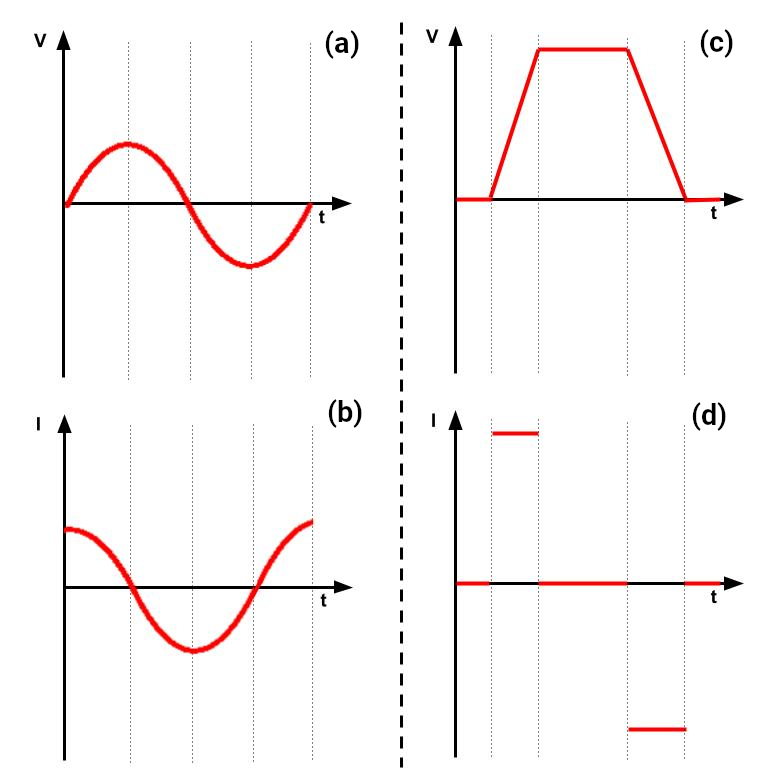
\includegraphics[scale=1.0]{./figures/Figure_5d4.png}}
\caption{Voltage/current waveforms for a purely capacitive circuit. For an input sinewave voltage (a), the resulting current waveform is given by (b). For an input trapezoidal voltage (c), the resulting current waveform in the circuit is (d).}
\label{fig5d4}
\end{figure}


\noindent \textit{Numerical Approaches for Calculating the Electric Field - Analytical approach.} The electrical circuit model described in the previous section can be used to calculate the \acs{EF} in the culture medium for a cylindrical geometry and a sinusoidal applied voltage. The described equations can be easily implemented in Excel, Matlab, or Python, for example. When the waveform is not sinusoidal, an estimate of the maximum \acs{EF} strength can be obtained by considering a frequency such that the maximum rates of change with time of the actual voltage waveform and a sinusoidal waveform of equal amplitude match. For example, for a linear ramp of amplitude $A$ and risetime $\tau$, consider a sinusoidal voltage of amplitude $A$ and frequency $f$. Then, equaling the maximum rates of change of these two waveforms gives the matching frequency:

\begin{equation}
\label{eqFrequency}
\frac{A}{\tau} = 2 \pi f A \quad or \quad f = \frac{1}{2 \pi \tau}
\end{equation}

The proposed analytical approach will yield estimates of the \acs{EF} of the right order of magnitude even when the geometry is non-cylindrical. However, appropriate care must be taken to choose equivalent dimensions for the cylindrical model. Specifically, the thickness of the insulating layers in the cylindrical model should be the same as in the original setup. \hfill \break


\begin{figure}
\makebox[\textwidth][c]{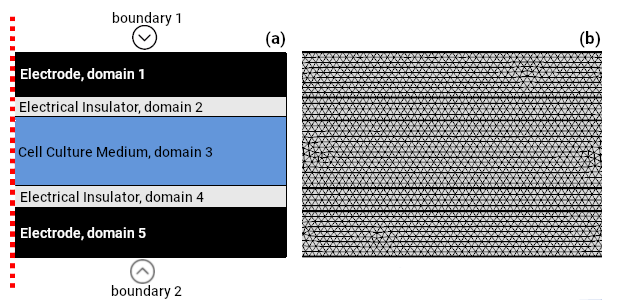
\includegraphics[scale=2.0]{./figures/Figure_5d5.png}}
\caption{Axisymmetric representation of a typical \acs{CCoupled} electric stimulation setup. (a) Domain identification of each layer and electrical boundary conditions applied at the electrodes for \acs{FEM} analysis; (b) Example of a physics-controlled mesh obtained in COMSOL using the extra fine option.}
\label{fig5d5}
\end{figure}

\noindent \textit{Numerical Approaches for Calculating the Electric Field - Circuit simulator approach.} As an alternative to the analytical approach, it is possible to use software packages for the simulation of analog circuits to view the temporal variation of the current or of the voltage drop in the culture medium and to estimate the \acs{EF} strength in the region of interest. We used the freely distributed program LTspice (LTspice LVII, Analog Devices, USA) to draw a circuit like the one illustrated in Fig.\ref{fig5d3}c considering only the 3 central sections since the impedance of the electrodes is negligible. The voltage waveform was specified as a sinusoidal waveform using the SINE option, as a trapezoidal pulse using the PULSE option, or as an arbitrary waveform using the PWL (piece-wise linear) option. After running the simulation, an LTspice probe tool was used to obtain the current through the resistive branch of the culture medium, from which the voltage drop and hence the \acs{EF} were calculated. Note that if using a circuit like the one illustrated in Fig.\ref{fig5d3}d for these simulations, the resistive and capacitive impedances of the various layers were calculated based on a single, matching frequency obtained as outlined in equation \ref{eqFrequency}. The two approaches should therefore provide the same estimates for the \acs{EF}. Additionally, this implies that the simulator does not consider the full frequency spectrum of the waveform and so the predicted temporal variations are not exact but rather good approximations of the true variations. \hfill \break

\noindent \textit{Numerical Approaches for Calculating the Electric Field - \acs{FEM} approach.} If the geometry of the setup makes it difficult to estimate the resistance and capacitance of the various layers, then a numerical method considering the specific features of the geometry should be applied to obtain accurate estimates of the \acs{EF}. In this study, we used the finite element method for this purpose. The setup geometry was defined previously in SolidWorks (version 2018, Dassault Systemes SolidWorks Corporation, France) and imported into COMSOL Multiphysics (version 5.2a, www.comsol.com, Stockholm, Sweden), where an extra fine, physics-controlled volume mesh was created, also enabling adaptive mesh refinement to guarantee mesh independent results. The \textit{Electric Currents} interface of the AC/DC module was used to solve the underlying partial differential equations, with the direct solver \acs{MUMPS}. This interface solves Laplace’s equation $\nabla \cdot (\sigma \nabla \phi) = 0$, where $\phi$ is the electrostatic potential and $\sigma$ is the electric conductivity and calculates the gradient of the scalar potential to determine the induced \acs{EF}. A \textit{Frequency Domain} study was selected for sinusoidal voltages and a \textit{Time-Dependent} study for arbitrary waveforms. Note that no assumptions about the frequency spectrum of the voltage waveform are needed since the original waveform is used. The boundary conditions applied were \textit{Electric Potential} and \textit{Ground} for the two electrodes, \textit{Electric Insulation} for other external boundaries, and \textit{Current Conservation} for internal boundaries. COMSOL can also handle ideal cylindrical geometries easily and efficiently as 2D axisymmetric models, as shown in Fig. \ref{fig5d5}. 

The three proposed approaches are based on well-known physics and well-established numerical methods and can produce accurate estimates of the \acs{EF} for increasingly complex waveforms and geometries. They all assume that the quasi-electrostatic approximation holds. \hfill \break

\begin{figure}
\makebox[\textwidth][c]{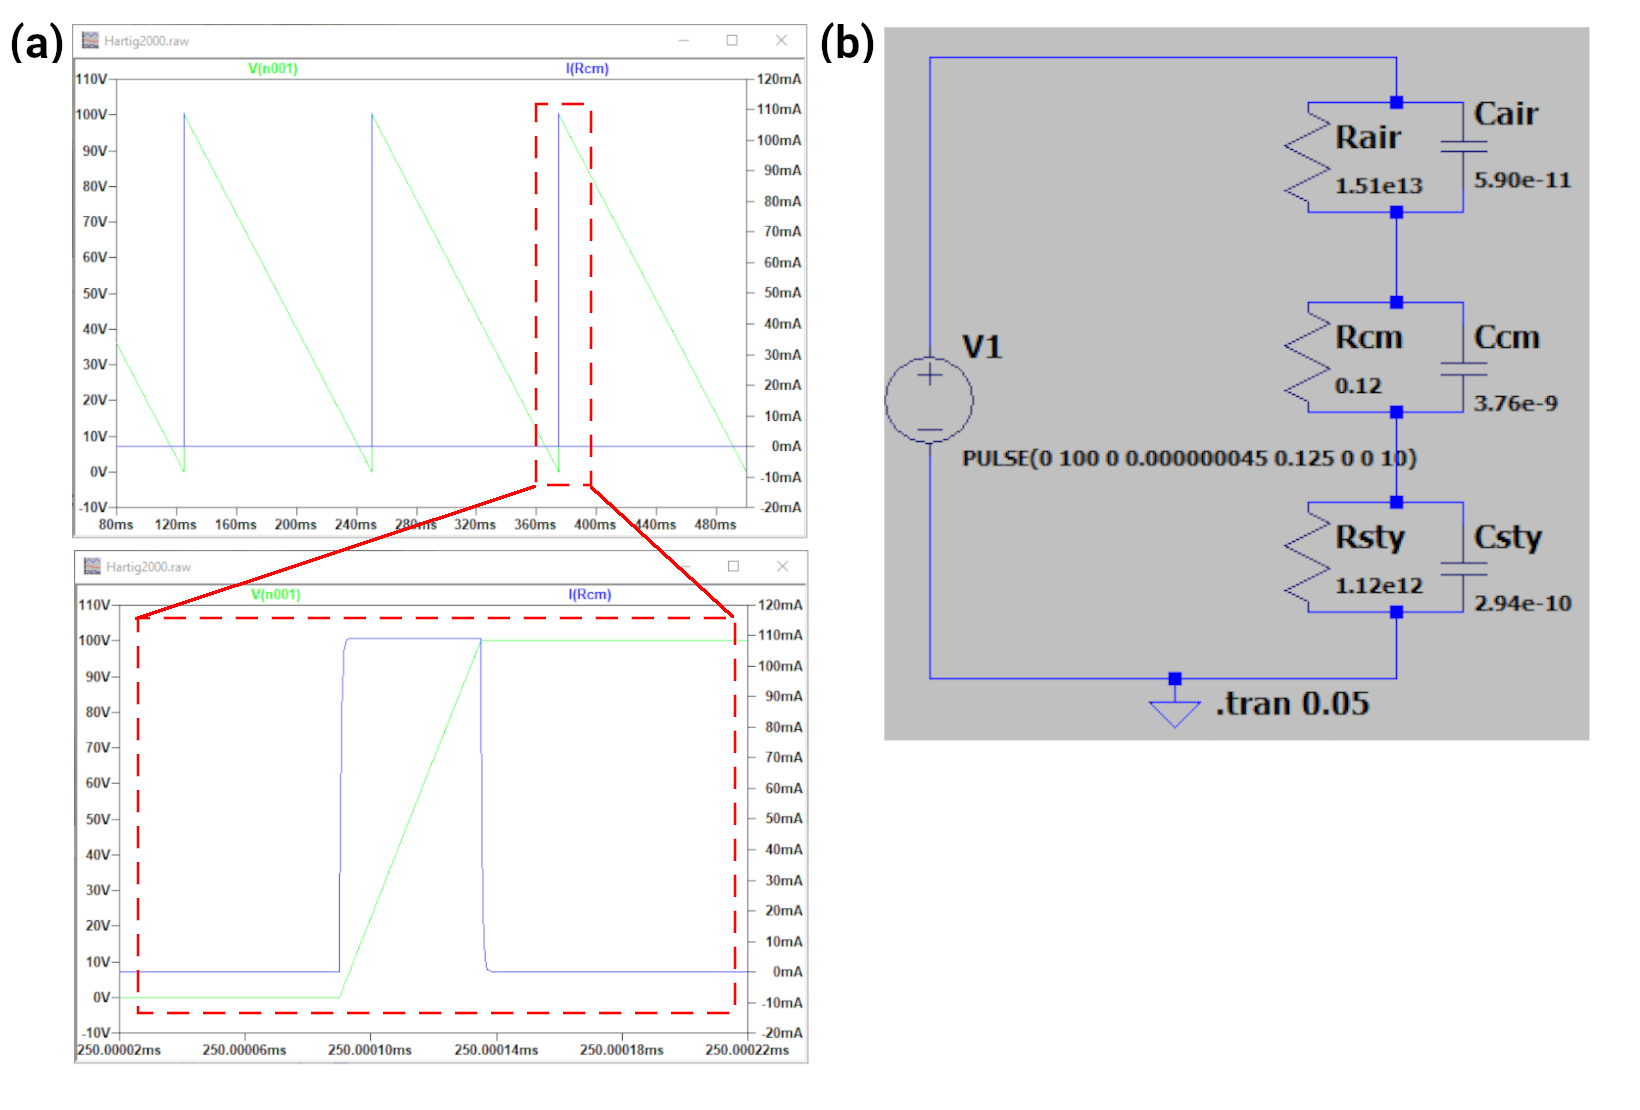
\includegraphics[scale=0.40]{./figures/Figure_5d6.png}}
\caption{Example of LTspice analog circuit simulation for Hartig's et al setup \cite{Hartig2000-ny}. Printscreens from the software environment: (a) digital probe tool visualizer showing the input potential signal (green line) and the electric current peak generated in the culture medium resistor (blue line). The bottom panel shows a detailed view of the rising edge for better visualization of the induced current; (b) the equivalent circuit model of Hartig's setup drawn in LTspice. Abbreviations: R-resistor, C-capacitor, cm-culture medium, sty-polystyrene, V1-voltage source.}
\label{fig5d6}
\end{figure}


\noindent \textit{Selection of studies and theoretical validation.} A bibliographic search was performed on ScienceDirect, Pubmed, and Scopus databases to identify experimental studies using \acs{CCoupled} stimulation. In order to narrow the search, only bone cell lineages were considered for this analysis, taking into consideration our research group's interest in bone tissue engineering. The following search sentence and keywords were considered:"(capacitive stimulation) AND (bone OR osteogenic OR osteogenesis) AND (in vitro)", originating a total of 922 records, 881 in ScienceDirect, 30 in Pubmed, and 11 in Scopus. After the removal of duplicates, the remaining 883 records were screened considering the following exclusion (e) and inclusion (i) criteria:

\begin{itemize}
\footnotesize
\item[(e1)] Publications consisting of reviews or studies \textit{in vivo}, or involving implants or prosthetic devices;
\item[(e2)] Studies targeting biological tissues other than bone;
\item[(e3)] Studies targeting cellular processes other than proliferation and differentiation;
\item[(e4)] Studies using stimulation phenomena other than capacitive coupling;
\item[(i1)] The geometry of the experimental setup and voltage waveform must be reported in sufficient detail to allow the construction of a reasonably accurate model; 
\item[(i2)] The cell culture chamber must be empty of any construct and contain only cellular content and culture medium;
\item[(i3)] The E-Field in the culture medium, measured or estimated, must be reported to allow a comparison with our model's predictions.
\end{itemize}

A total of 16 records fulfilled all criteria. 4 additional records fulfilling all criteria were found by hand searching the reference lists in the 16 records mentioned previously. Eight different setups for capacitive stimulation are reported in these 20 records. They are listed below and were named after the first author of the oldest reference.

\begin{itemize}
\footnotesize
\item  Rodan \textit{et al.}, 1978, original description of this setup \cite{Rodan1978-yu};
\item  Korenstein \textit{et al.}, 1984, original description of this setup \cite{Korenstein1984-qb}, also used in \cite{Laub1984-qm, Danon1984-eu, Binderman1985-mh, Ozawa1989-uz};
\item  Fitzsimmons \textit{et al.}, 1986, original description of this setup \cite{Fitzsimmons1986-ks}, also used in \cite{Fitzsimmons1989-zj, Fitzsimmons1992-vw}; 
\item  Brighton \textit{et al.} 1992, original description of this setup \cite{Brighton1992-gg}, also used in \cite{Armstrong1988-ob, Wang2006-hx, Brighton2008-rl, Clark2014-sz};
\item  Hartig \textit{et al.}, 2000, original description of this setup \cite{Hartig2000-ny}, also used in \cite{Wiesmann2001-uh};
\item  Griffin \textit{et al.}, 2011, original description of this setup \cite{Griffin2011-bb}, also used in \cite{Griffin2013-wp};
\item  Stephan \textit{et al.}, 2020, original description of this setup \cite{Stephan2020-qh};
\item  Khaw \textit{et al.}, 2021, original description of this setup \cite{Khaw2021-tv};
\end{itemize}

\noindent In all these studies, the \acs{EF} values reported were calculated, not measured.

For each one of these setups, the \acs{EF} in the culture medium was calculated using the three approaches described in the previous section. The analytical solutions were implemented in Matlab and Python. The use of LTspice is exemplified in Fig. \ref{fig5d6} with the asymmetric sawtooth voltage waveform applied in Hartig's setup \cite{Hartig2000-ny}. Rodan’s \cite{Rodan1978-yu}, Stephan's \cite{Stephan2020-qh}, and Khaw's \cite{Khaw2021-tv} setups are clearly different from the ideal layered cylindrical geometry. For these setups, a realistic geometry was implemented in COMSOL. Fig. \ref{fig5d7} shows the realistic model for Rodan's setup \cite{Rodan1978-yu}, together with the layered cylindrical model with similar dimensions for analytical and circuit simulator calculations.


\begin{figure}
\makebox[\textwidth][c]{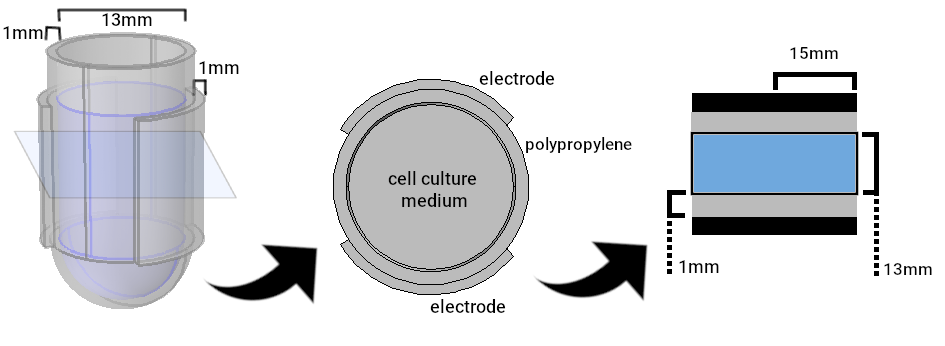
\includegraphics[scale=1.5]{./figures/Figure_5d7.png}}
\caption{\acs{3D} \acs{FEM} model created to replicate Rodan's et al. setup \cite{Rodan1978-yu} and the geometrical approximation considered for its equivalent electronic circuit model.}
\label{fig5d7}
\end{figure}




\section{Results}




\subsection{Scaffold insertion effects}

\noindent \textit{Validation of Brighton \acs{3D} \acs{FEM} model.} Brighton \textit{et al.} \cite{Armstrong1988-ob, Brighton1992-gg} reported that, with their experimental setup (performed in the absence of any scaffold structure) and using a 60 \si{\kilo\hertz} sinusoidal wave of  44.81 \si{\volt} amplitude, they were able to generate an electric field of 20 \si{\milli\volt\per\centi\meter} (2.0 \si{\volt\per\meter}) and a current density of 300 \si{\micro\ampere\per\square\centi\meter} (3.0 \si{\ampere\per\square\meter}). Our \acs{3D} \acs{FEM} model without scaffold predicts an average \acs{EF} of 2.1 \si{\volt\per\meter} and an average current density of 3.2 \si{\ampere\per\square\meter}  in the culture medium. Thus, by comparison, we can conclude that this \acs{3D} \acs{FEM} model accurately predicts the values obtained experimentally in Brighton \textit{et al.} \cite{Armstrong1988-ob, Brighton1992-gg} considering a chamber filled with culture medium and in the absence of a scaffold structure. \hfill \break

\noindent \textit{Sensitivity Analysis.} The sensitivity analysis was performed on the results obtained for Brighton's setup, including the scaffold structure. Sensitivity analysis results from the Delta Moment-Independent Measure are shown in Table \ref{table_delta}. The higher the First Order significance, the greater the contribution of the corresponding parameter to the variation of the electric field magnitude. As expected, in the external \acs{ROI}, the conductivity of the culture medium has the greatest impact on the electric field. Conversely, in the internal \acs{ROI}, the scaffold's conductivity has the greatest impact, followed by the conductivity of the culture medium.


\begin{table}
\caption{ Delta Moment-Independent Measure Results.}
\bigskip
\small
\centering
\begin{tabularx}{405px}{l c c c c c} \toprule[0.15em]
\textbf{ROI} & \textbf{parameter} & \textbf{delta} & \textbf{confidence} & \textbf{1st order significance} & \textbf{ confidence} \\ \cmidrule(l){1-6}
EXTERNAL & $\sigma_{cm}$ &  0.58 & 0.02 & 0.64 & 0.04 \\
& $\epsilon_{cm}$ & 0.28 & 0.01 & 0.17 & 0.01\\
& $\sigma_{s}$  & 0.09 & 0.01 & 0.09 & 0.05\\
& $\epsilon_{s}$ & 0.28 & 0.01 & 0.17 & 0.01 \\ \cmidrule(l){1-6}
INTERFACE & $\sigma_{cm}$ &  0.51 & 0.02 & 0.63 & 0.06 \\
& $\epsilon_{cm}$ & 0.20 & 0.01 & 0.09 & 0.01\\
& $\sigma_{s}$  & 0.40 & 0.03 & 0.68 & 0.03\\
& $\epsilon_{s}$ & 0.20 & 0.01 & 0.09 & 0.01 \\ \cmidrule(l){1-6}
INTERNAL & $\sigma_{cm}$ &  0.39 & 0.02 & 0.45 & 0.04 \\
& $\epsilon_{cm}$ & 0.13 & 0.01 & 0.04 & 0.01\\
& $\sigma_{s}$  & 0.53 & 0.03 & 0.84 & 0.03\\
& $\epsilon_{s}$ & 0.13 & 0.01 & 0.04 & 0.01 \\ \bottomrule[0.15em]
\end{tabularx}
\label{table_delta}
\end{table}


Sensitivity analysis on \acs{FEM} solutions from the parametric sweep study were plotted and grouped by color code in Figure \ref{fig5d8}, with different colors representing different electrical conductivities of the culture medium. Each row shows plots of the average, maximum, and minimum \acs{EF} magnitude in one of the three \acs{ROI}s as a function of the electrical conductivity of the scaffold. Variations in the relative permittivities of the culture medium and scaffold had no noticeable impact on the \acs{EF}. Hence, a single point in these graphs represents the value of the \acs{EF} for all values of the permittivities.


\begin{figure}
\makebox[\textwidth][c]{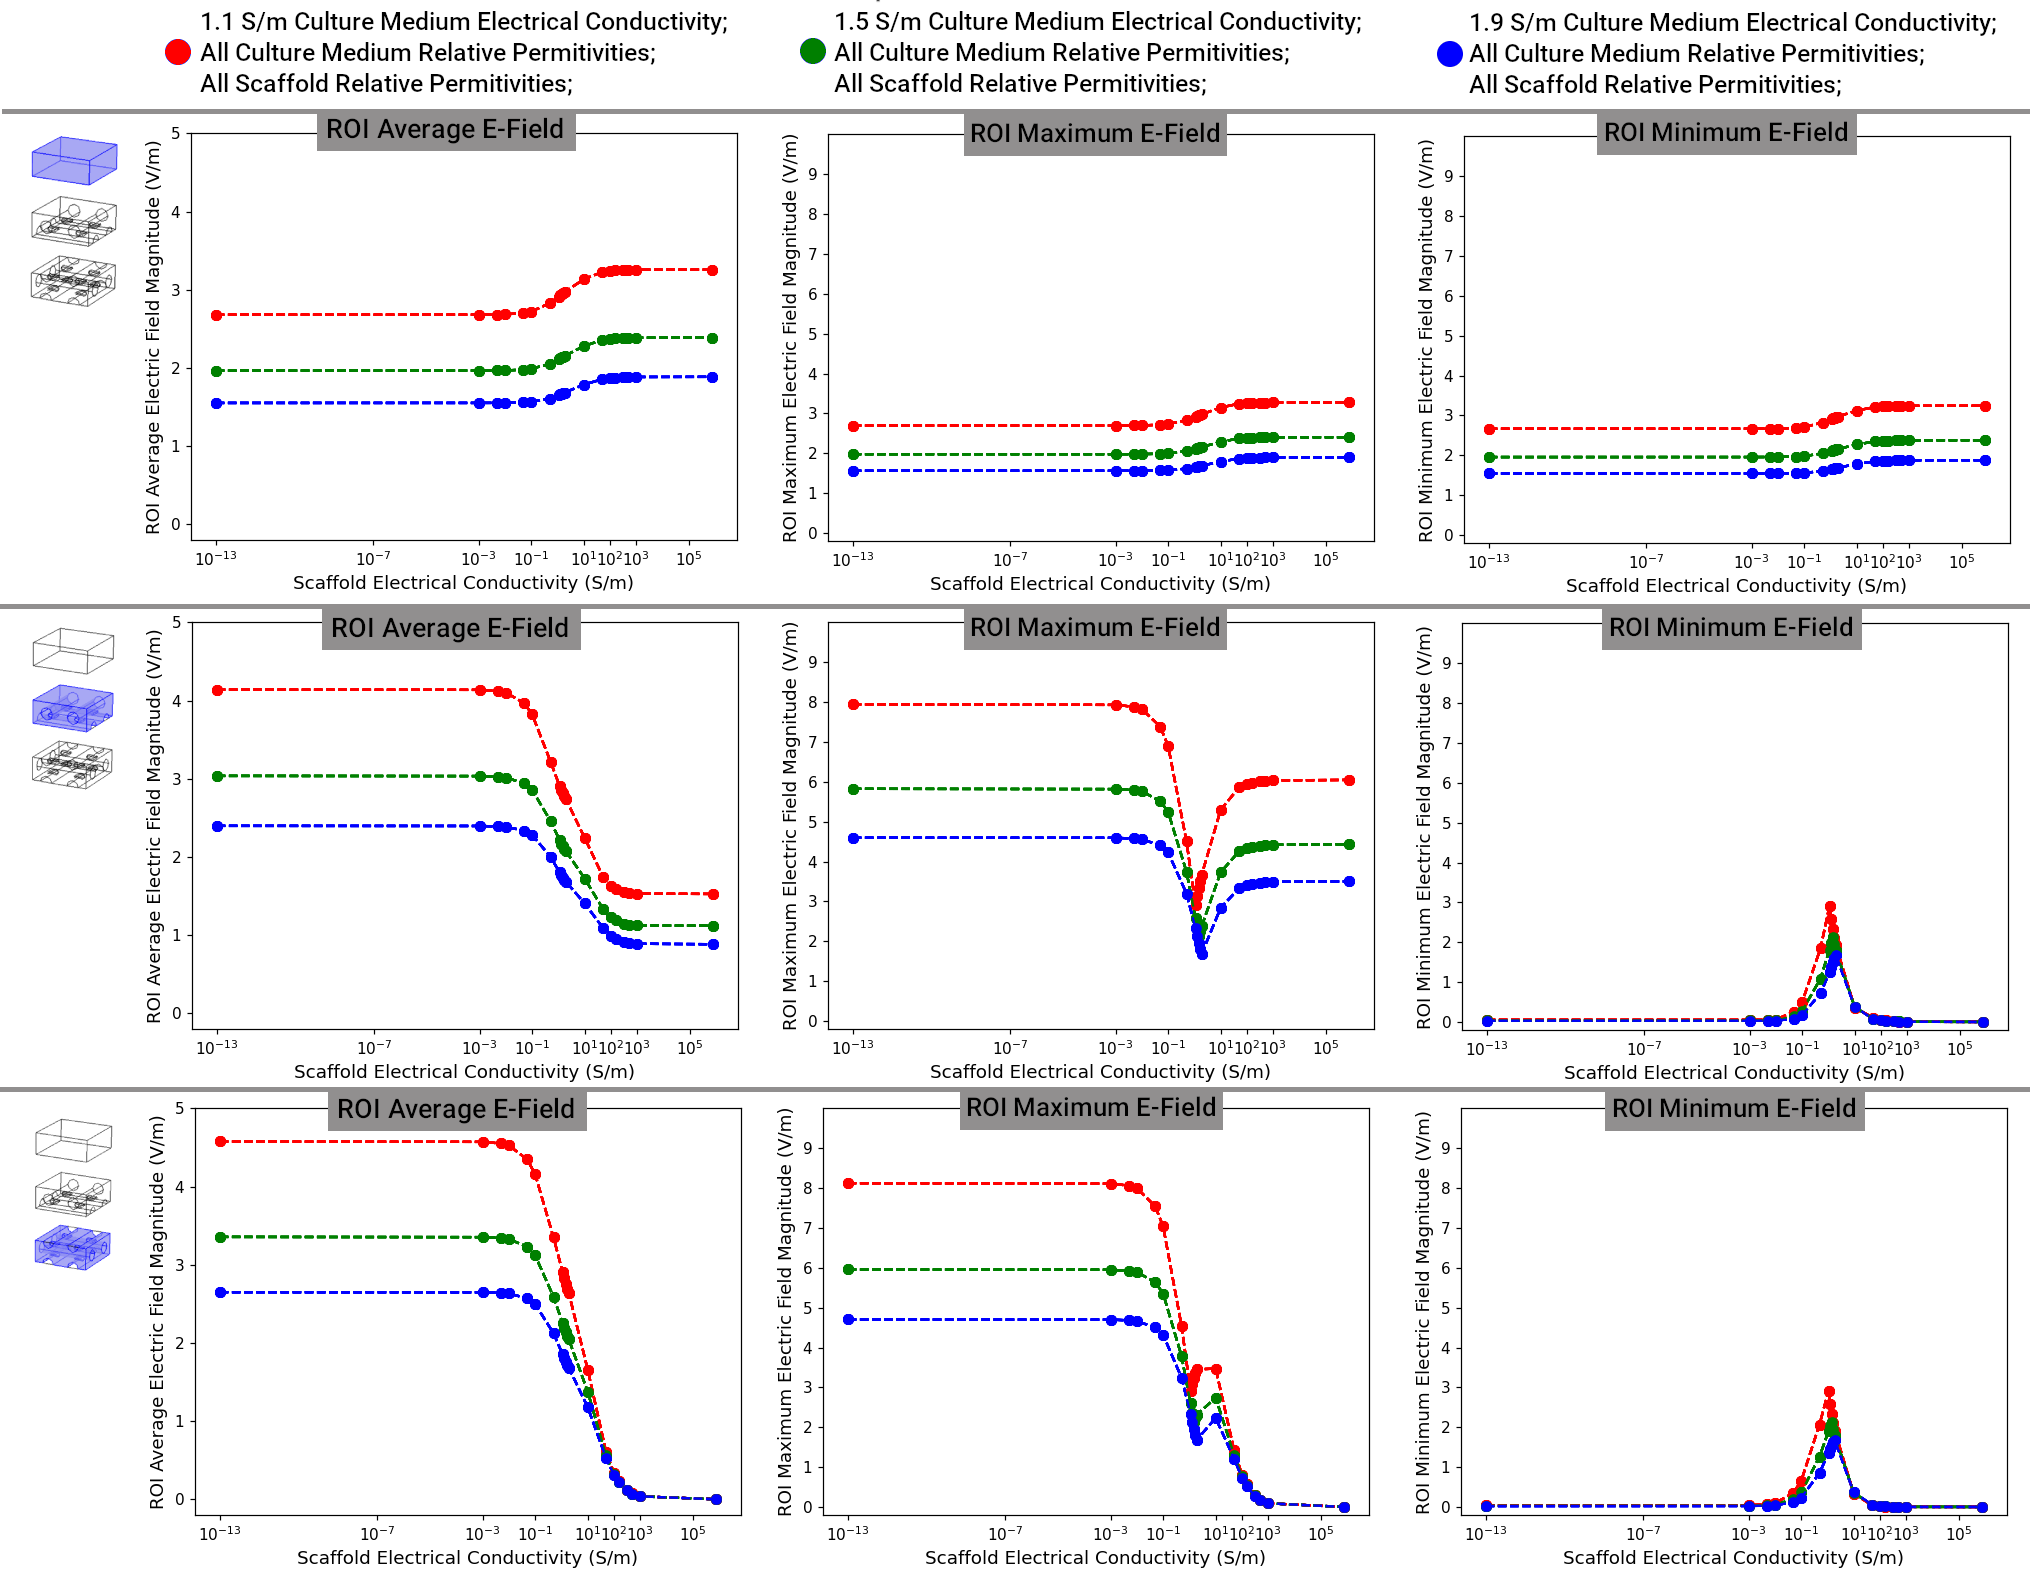
\includegraphics[scale=1.0]{./figures/Figure_5d8.png}}
\caption{One-at-a-time sensitivity analysis of the electric field magnitude per region-of-interest. Each row contains plots for the average, maximum, and minimum electrical field versus the scaffold material's electrical conductivity. Each plot contains all 540 different solutions (each solution is represented by one point), and data are color-coded by culture medium electrical conductivity. The plotted data under analysis only contains solutions from the culture medium nodes.}
\label{fig5d8}
\end{figure}


\noindent We can observe that at 60 \si{\kilo\hertz} the parameters that most influence the magnitude of the \acs{EF} in a bioreactor are the electrical conductivities of both the culture medium and the scaffold material. All plots in Figure \ref{fig5d8} analysis may be split into three regions: one region corresponding to insulating materials with electrical conductivity lower than \num{1.0d-2} \si{\siemens\per\meter}, where changes in scaffold electrical conductivity generate small variations in the \acs{EF}, for a fixed cell culture medium conductivity; another region corresponding to conductive materials with electrical conductivity greater than \num{1.0d2} \si{\siemens\per\meter}, where changes in scaffold electrical conductivity generate small variations in the \acs{EF}; and a transition region, where an almost linear relation between scaffold electrical conductivity and the \acs{EF} magnitude can be observed in the average plots (left column of Figure \ref{fig5d8}). On the other hand, in the maximum and minimum plots, local minima and maxima arise when the electrical conductivity of the scaffold matches that of the cell culture medium (see Figure \ref{fig5d8}). \hfill \break


\noindent \textit{Spatial Distribution Analysis.} Spatial distributions of the \acs{EF} magnitude are presented in Figure \ref{fig5d9}. As expected, the control scaffold, which was considered with the same electrical properties as the cell culture medium, introduces no changes in the predicted \acs{EF}, which remains uniform (Figure \ref{fig5d9} - A1, B1, C1, H1). When the scaffold is more insulating or more conductive than the cell culture medium, the \acs{EF} distribution is greatly affected. A more insulating scaffold material generates local hot zones and cold zones inside the scaffold (Figure \ref{fig5d9} - A2, B2, C2, H2, A3, B3, C3, H3). A more conductive scaffold material shields the surrounding culture medium from the external \acs{EF} stimulation (Figure \ref{fig5d9} - A4, B4, C4, H4). The histograms in the bottom row show that the presence of insulating scaffolds spreads the range of the delivered \acs{EF} magnitude, while the presence of conductive scaffolds reduces this range.


\begin{sidewaysfigure}
\makebox[\textwidth][c]{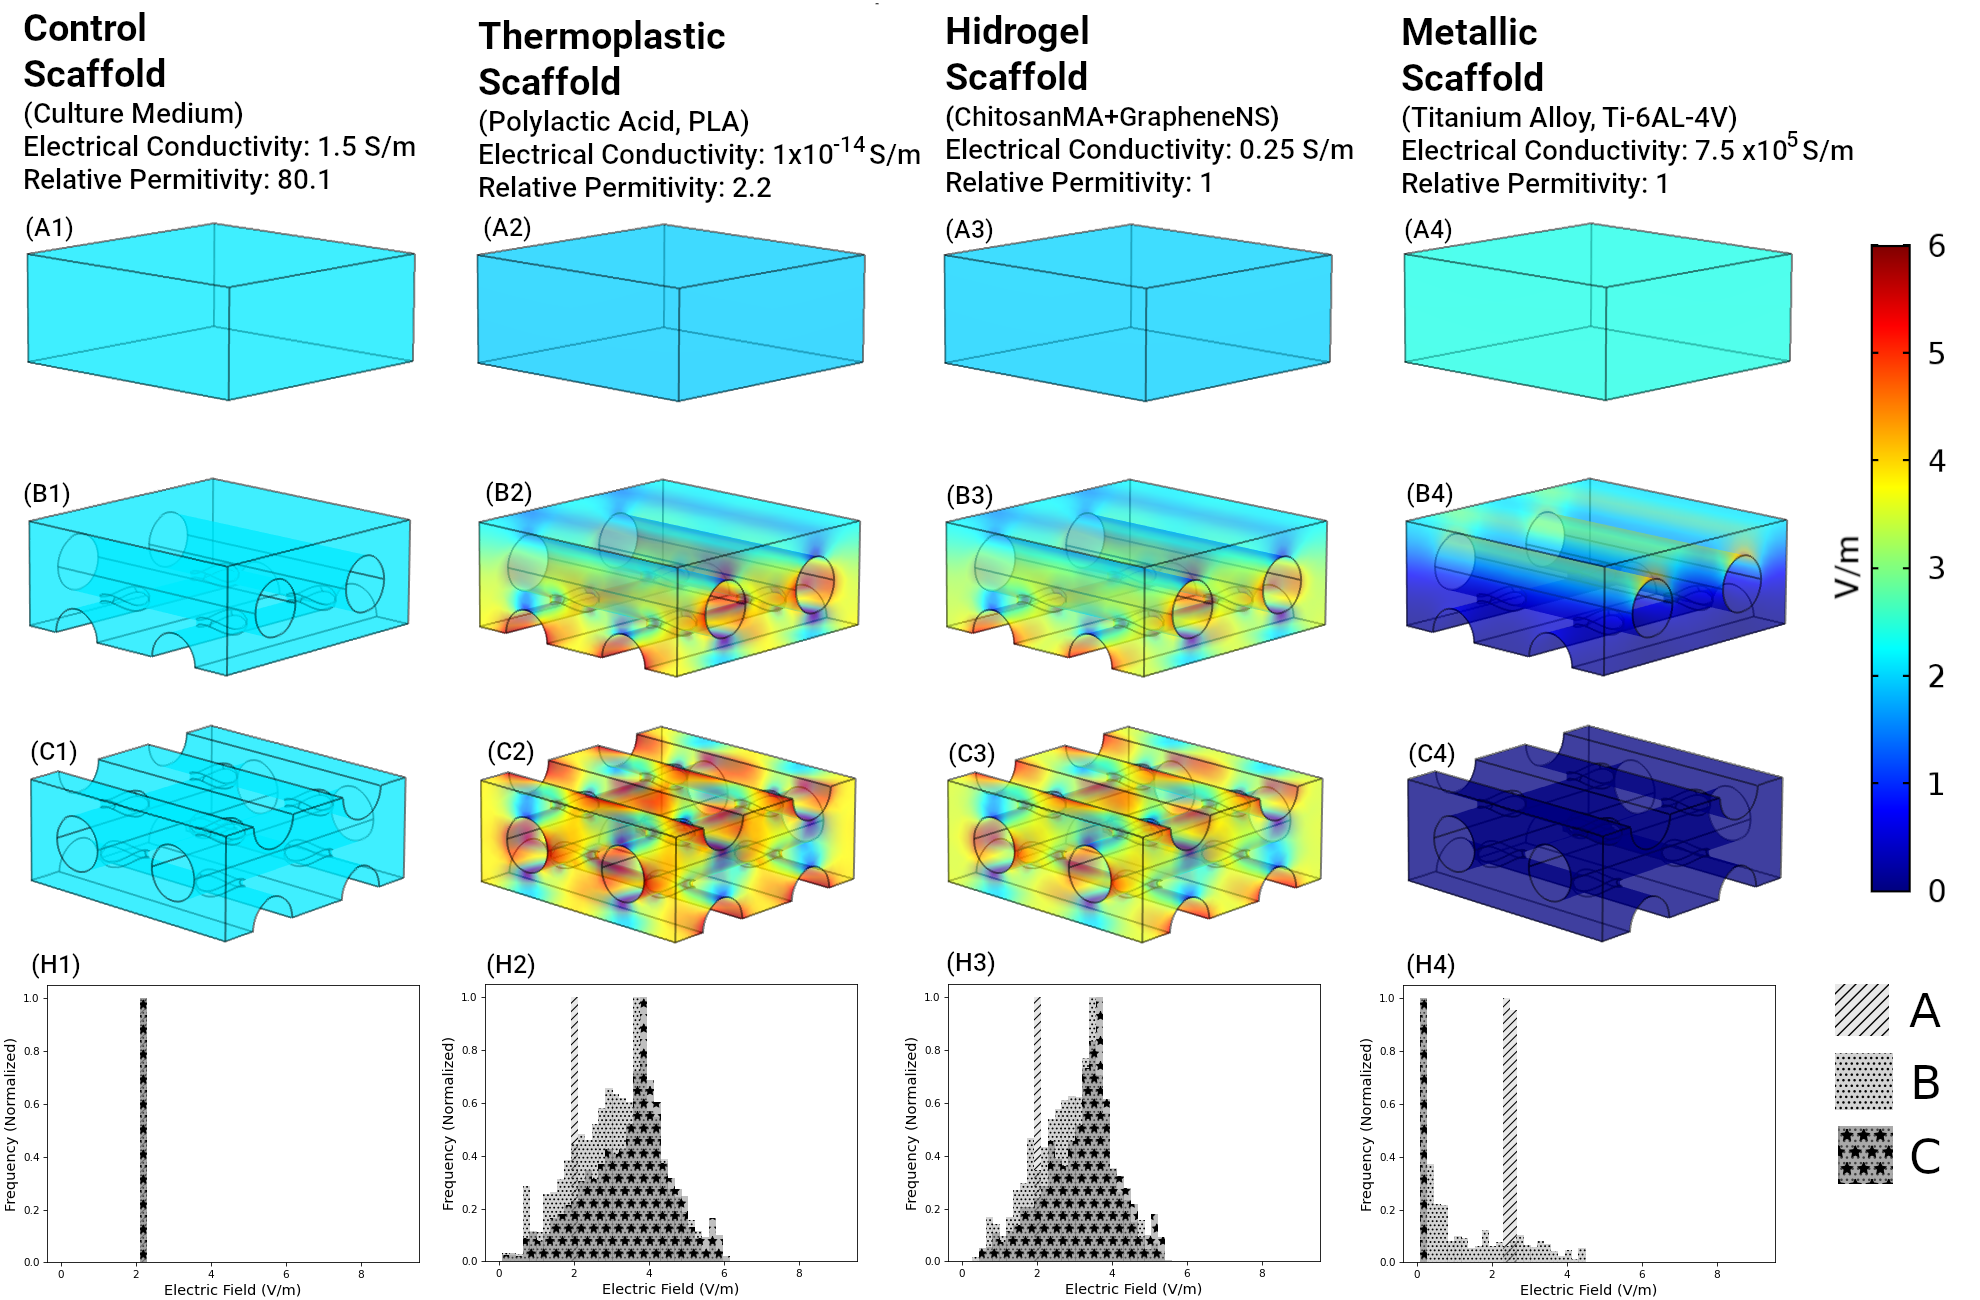
\includegraphics[scale=1.0]{./figures/Figure_5d9.png}}
\caption{Spatial distribution of the \acs{EF} under fixed culture medium electrical parameters ($\sigma$: \num{1.5} \si{\siemens\per\meter}, $\epsilon_r$: 80.1) and fixed external electric stimulation (Brighton's conditions). Each column of the figure presents the predicted result for the specified scaffold material at the \acs{ROI}s labeled from A to C. A normalized frequency histogram of the \acs{EF} magnitude is presented in the bottom row.}
\label{fig5d9}
\end{sidewaysfigure}


\newpage
\subsection{Modelling \acs{CCoupled} reported setups}


Modelling data like the dimensions of the setup, the values of the electrical properties of the materials, and details of the voltage waveform for all eight studies are compiled in Table \ref{table_prop}. Note that the inverse of resistivity, i.e., the conductivity, $\sigma$, is listed in this table. Reasonable estimates for missing values were obtained from the literature presented in the table. The resistance, capacitance, and reactance of the three central layers of each setup were calculated based on these values and are also listed in Table \ref{table_electro}. Khaw's setup is not listed in this table because, at zero frequency, the capacitive reactance of the insulators is infinite (Equation \ref{eqCimpedance}), so the current through the setup and hence the \acs{EF} in the culture medium will be zero.


\begin{table}[p]
\caption{Dimensions, materials electrical properties, and waveforms for each of the setups modeled. $\epsilon_{r}$ represents the relative permittivity, whereas $\sigma$ represents the electric conductivity.}
\bigskip
\tiny
\centering
\begin{tabularx}{\textwidth}{l l l l} \toprule[0.15em]
\textbf{Setup} & \textbf{Dimensions} & \textbf{Materials and Electrical Properties} & \textbf{Waveform} \\ \cmidrule(l){1-4}

Rodan \textit{et al.}, & radius: 15\si{\milli\meter} & \textit{layers 1,4:} 	& Positive trapezoidal pulse,\\
1978 \cite{Rodan1978-yu} & \textit{layers 1,4:} thickness - 1 \si{\milli\meter} & Copper: $\epsilon_{r}$=1; $\sigma$=5.998e7 S/m & 1750 \si{\volt} amplitude,\\
& \textit{layer 2:} thickness - 1 \si{\milli\meter} & \textit{layer 2:} & 0.1 \si{\second} pulse width,\\
& \textit{layer 3:} thickness - 13 \si{\milli\meter} & Polypropylene: $\epsilon_{r}$=2.1; $\sigma$=1e-16 S/m \cite{IneosPP} & 1.85 \si{\milli\second} fall/rise time \\
&  & \textit{layer 3:} &\\
&  & Culture Medium: $\epsilon_{r}$=80.1; $\sigma$=1.5 S/m \cite{Visone2018-sa} & \\ \cmidrule(l){1-4}


Korenstein \textit{et al.}, & radius: 27 \si{\milli\meter} & \textit{layers 1,5:} & \\
 1984 \cite{Korenstein1984-qb} & \textit{layers 1,5:} thickness - 1 \si{\milli\meter} &  Copper: $\epsilon_{r}$=1; $\sigma$=\num{5.99d7} \si{\siemens\per\meter} & Negative trapezoidal pulse, \\
& \textit{layer 2:} thickness - 1.25 \si{\milli\meter} & \textit{layer 2:}  & 300 \si{\volt}, 500 \si{\volt}  \\
& \textit{layer 3:} thickness - 2.25 \si{\milli\meter} &  Air: $\epsilon_{r}$=1.005; $\sigma$=\num{1.0d-14} \si{\siemens\per\meter} & and 1300 \si{\volt} amplitude, \\
& \textit{layer 4:} thickness - 1 \si{\milli\meter} & \textit{layer 3:} &25 \si{\micro\second} pulse width, \\
& & Culture Medium: $\epsilon_{r}$=74; $\sigma$=\num{1.5} \si{\siemens\per\meter} \cite{Korenstein1984-qb, Visone2018-sa} &  7 \si{\nano\second} fall/rise time \\
&  & \textit{layer 4:} & \\
& & Polystyrene: $\epsilon_{r}$=2.5; $\sigma$=\num{6.7d-14} \si{\siemens\per\meter} \cite{Qi2011-se} & \\ \cmidrule(l){1-4}


Fitzsimmons \textit{et al.},  & radius: 26\si{\milli\meter} & \textit{layers 1,5:} & \\
1985 \cite{Fitzsimmons1986-ks} & \textit{layers 1,5:}  thickness - 1 \si{\milli\meter} & Metal Plates: $\epsilon_{r}$=1; $\sigma$=\num{5.99d7} \si{\siemens\per\meter} & Sinusoidal wave, \\
& \textit{layer 2:} thickness - 10 \si{\milli\meter} & \textit{layer 2:} & 10 \si{\volt} amplitude, 10 \si{\hertz} \\
& \textit{layer 3:} thickness - 7 \si{\milli\meter} & Air: $\epsilon_{r}$=1.005; $\sigma$=\num{1.0d-14} \si{\siemens\per\meter} \cite{Seran2017-qg} & \\
& \textit{layer 4:} thickness - 3 \si{\milli\meter} & \textit{layers 3:} & \\
& & Culture Medium: $\epsilon_{r}$=80.1; $\sigma$=1.5 S/m \cite{Visone2018-sa} & \\
& & \textit{layer 4:} & \\
& & Polystyrene: $\epsilon_{r}$=2.5; $\sigma$=\num{6.7d-14} \si{\siemens\per\meter} \cite{Qi2011-se} & \\ \cmidrule(l){1-4}


Brighton \textit{et al.},  & radius: 16.5 \si{\milli\meter} & \textit{layers 1,5:}  & \\
1992 \cite{Brighton1992-gg} & \textit{layers 1,5:} thickness - 1 \si{\milli\meter} & Stainless Steel: $\epsilon_{r}$=1; $\sigma$=\num{4.032d6} \si{\siemens\per\meter} & Sinusoidal Wave, \\
& \textit{layers 2, 4:} thickness - 0.16 \si{\milli\meter} & \textit{layers 2, 4:} & 44.81 \si{\volt} amplitude,\\
& \textit{layer 3:} thickness - 9.8 \si{\milli\meter} & No.1 Glass Coverslip: $\epsilon_{r}$=6.85; $\sigma$=\num{1d-13} \si{\siemens\per\meter} \cite{Hench1972-el} & 60 \si{\kilo\hertz} \\
&  & \textit{layers 3:} & \\
&  & Culture Medium: $\epsilon_{r}$=80.1; $\sigma$=1.5 \si{\siemens\per\meter} \cite{Visone2018-sa} & \\ \cmidrule(l){1-4}
 

Hartig \textit{et al.}, & radius: 65 \si{\milli\meter} & \textit{layers 1,5:} & \\
2000 \cite{Hartig2000-ny} & \textit{layers 1,5:} thickness - 2 \si{\milli\meter} & High Grade Stainless Steel: $\epsilon_{r}$=1; $\sigma$=\num{0.14d7} \si{\siemens\per\meter} & Asymmetric sawtooth, \\
& \textit{layer 2:} thickness - 2 \si{\milli\meter} & \textit{layer 2:} & 100 \si{\volt} peak-to-peak, 	\\
& \textit{layer 3:} thickness - 2.5 \si{\milli\meter} & Air: $\epsilon_{r}$=1.005;  $\sigma$=\num{1.0d-14} \si{\siemens\per\meter} \cite{Seran2017-qg} & 45 \si{\nano\second} risetime, \\
& \textit{layer 4:} thickness - 1 \si{\milli\meter} & \textit{layer 3:} & 62.5 \si{\milli\second} falltime	\\
& & Culture Medium: $\epsilon_{r}$=80.1;  $\sigma$=1.5 \si{\siemens\per\meter} \cite{Visone2018-sa} & \\
& & \textit{layer 4:} & \\
&  & Polystyrene: $\epsilon_{r}$=2.5;  $\sigma$=\num{6.7d-14} \si{\siemens\per\meter} \cite{Qi2011-se} & \\ \cmidrule(l){1-4}


Griffin \textit{et al.}, & radius: 40 \si{\milli\meter} & \textit{layers 1,5:} & \\
 2011 \cite{Griffin2011-bb} & \textit{layers 1,5:} thickness - 1 \si{\milli\meter} & High Grade Steel: $\epsilon_{r}$=1; $\sigma$=\num{5.99d7} \si{\siemens\per\meter} & Degenerate Wave, \\
& \textit{layer 2:} thickness - 2 \si{\milli\meter} & \textit{layer 2:} & 160 \si{\milli\volt} peak-to peak,\\
& \textit{layer 3:} thickness - 4.7 \si{\milli\meter} &  Air: $\epsilon_{r}$=1.005; $\sigma$=\num{1d-14} \si{\siemens\per\meter} \cite{Seran2017-qg} & 62.5 \si{\milli\second} duration,\\
& \textit{layer 4:} thickness - 1 \si{\milli\meter} & \textit{layer 3:} & 16 \si{\hertz}\\
&  & Culture Medium: $\epsilon_{r}$=80.1; $\sigma$=1.5 \si{\siemens\per\meter} \cite{Visone2018-sa} & \\
&  & \textit{layer 4:} & \\
& & Polystyrene: $\epsilon_{r}$=2.5; $\sigma$=6.7e-14 S/m \cite{Qi2011-se} & \\ \cmidrule(l){1-4}


Stephan \textit{et al.}, & 3D Model, radius: 16 \si{\milli\meter} & \textit{layers 1,5:} & \\
2020 \cite{Stephan2020-qh} & \textit{layers 1,5:} thickness - 0.5 \si{\milli\meter} & Ti6Al4V: $\epsilon_{r}$=1; $\sigma$=\num{5.85d5} \si{\siemens\per\meter} \cite{Mitchell2004-ue} & Sinusoidal Wave, \\
& \textit{layer 2,4:}  thickness - 1 \si{\milli\meter} & \textit{layer 2:} & 1.41 \si{\volt} and \\
& \textit{layer 3:} thickness - 32 \si{\milli\meter} & Polystyrene: $\epsilon_{r}$=2.5; $\sigma$=\num{6.7d-14} \si{\siemens\per\meter} \cite{Qi2011-se} & 0.141 \si{\volt} amplitude, \\
& & \textit{layer 3:} & 60 \si{\kilo\hertz} \\
&  & Culture Medium: $\epsilon_{r}$=80.1 \cite{Visone2018-sa}; $\sigma$=1.6 \si{\siemens\per\meter} & \\ \cmidrule(l){1-4}


Khaw \textit{et al.}, & 3D Model, radius: 15 \si{\milli\meter} & \textit{layers 1,5:} & \\
 2021 \cite{Khaw2021-tv} & \textit{layers 1,5:}  thickness - 1.75 \si{\milli\meter} & Electrode: $\epsilon_{r}$=1; $\sigma$=\num{5.99d7} \si{\siemens\per\meter} & Constant Potential \\
& \textit{layer 2,4:} & \textit{layer 2,4:} & 14.2 \si{\volt} and 28.4 \si{\volt},\\
& thickness - 0.75 \si{\milli\meter} & Plastic: $\epsilon_{r}$=2; $\sigma$=\num{6.7d-14} \si{\siemens\per\meter} \cite{Qi2011-se} & \\
& \textit{layer 3:}  thickness - 19.5 \si{\milli\meter} & \textit{layer 3:} & \\
& & Culture Medium: $\epsilon_{r}$=80; $\sigma$=1.7 \si{\siemens\per\meter} & \\
& \textit{air sphere (3D model only):} & \textit{air sphere (3D model only):} & \\
& radius: 120 \si{\milli\meter} & Air: $\epsilon_{r}$=1; $\sigma$=\num{1d-14} \si{\siemens\per\meter} \cite{Seran2017-qg} & \\ \bottomrule[0.15em]
\end{tabularx}
\label{table_prop}
\end{table}



\begin{table}
\caption{Values of the resistances, capacitances, reactances, and frequencies for the three-layer analog circuit models of the \acs{CCoupled} setups.}
\bigskip
\scriptsize
\centering
\begin{tabularx}{410px}{l l l l l l} \toprule[0.15em]
\textbf{Setup} & \textbf{Layers} &\textbf{ Resistance} &\textbf{Capacitance} &\textbf{Reactance} & \textbf{Frequency} \\ \cmidrule(l){1-6}

Rodan \textit{et al.}, & Layer 1 - Polypropylene & \num{1.41d16} \si{\ohm} & \num{1.31d-11} \si{\farad} &\num{-1.41d8}\si{\ohm} & 86.03 \si{\hertz}** \\
1978  \cite{Rodan1978-yu} & Layer 2 - Culture Medium & \num{12.26} \si{\ohm} & \num{3.86d-11} \si{\farad}	&\num{-4.80d7}\si{\ohm} & \\
& Layer 3 - Polypropylene & \num{1.41d16} \si{\ohm} & \num{1.31d-11} \si{\farad} &\num{-1.41d8}\si{\ohm} & \\ \cmidrule(l){1-6}

Korenstein \textit{et al.}, & Layer 1 - Air & \num{5.46d13} \si{\ohm} & \num{1.63d-11} \si{\farad} &\num{-4.29d2}\si{\ohm} & 22.7 \si{\mega\hertz}**	\\
1984 \cite{Korenstein1984-qb} & Layer 2 - Culture Medium & \num{0.65} \si{\ohm} & \num{6.67d-10} \si{\farad} &\num{-0.10d2}\si{\ohm} & \\
& Layer 3 - Polystyrene & \num{6.52d12} \si{\ohm} & \num{5.07d-11} \si{\farad} &\num{-1.38d2}\si{\ohm} & \\ \cmidrule(l){1-6}

Fitzsimmons \textit{et al.}, & Layer 1 - Air & \num{4.71d14} \si{\ohm} & \num{1.89d-12} \si{\farad}	&\num{-8.42d9}\si{\ohm} & 10 \si{\hertz} \\
1985 \cite{Fitzsimmons1986-ks} & Layer 2 - Culture Medium & \num{2.20} \si{\ohm} & \num{2.15d-10} \si{\farad} &\num{-7.40d7} \si{\ohm} & \\
& Layer 3 - Polystyrene & \num{2.11d13} \si{\ohm} & \num{1.57d-11} \si{\farad} &\num{-1.02d9}\si{\ohm} & \\ \cmidrule(l){1-6}

Brighton \textit{et al.}, & Layer 1 - No.1 Glass Coverslip & \num{1.87d12} \si{\ohm} & \num{3.24d-10} \si{\farad} &\num{-8.18d3} \si{\ohm} & 60 \si{\kilo\hertz} \\
1992  \cite{Brighton1992-gg} & Layer 2 - Culture Medium & \num{7.79} \si{\ohm} & \num{6.07d-11} \si{\farad} &\num{-4.37d4}\si{\ohm} & \\
& Layer 3 - No.1 Glass Coverslip & \num{1.87d12} \si{\ohm} & \num{3.24d-10} \si{\farad} &\num{-8.18d3}\si{\ohm}	& \\ \cmidrule(l){1-6}

Hartig \textit{et al.}, & Layer 1 - Air & \num{1.51d13} \si{\ohm} & \num{5.91d-11} \si{\farad}	&\num{-7.62d2}\si{\ohm} & 3.5 \si{\mega\hertz}** \\
2000 \cite{Hartig2000-ny} & Layer 2 - Culture Medium & \num{0.13} \si{\ohm} & \num{3.76d-09} \si{\farad} &\num{-1.20d1}\si{\ohm} & \\
& Layer 3 - Polystyrene & \num{1.12d12} \si{\ohm} & \num{2.94d-10} \si{\farad} &\num{-1.53d2}\si{\ohm} & \\ \cmidrule(l){1-6}

Griffin \textit{et al.}, & Layer 1 - Air & \num{3.98d13} \si{\ohm} & \num{2.24d-11} \si{\farad}	&\num{-3.23d8}\si{\ohm} & 22 \si{\hertz} \\
 2011 \cite{Griffin2011-bb} & Layer 2 - Culture Medium & \num{0.62}  \si{\ohm} & \num{7.58d-10} \si{\farad}	&\num{-9.54d6}\si{\ohm} & \\
& Layer 3 - Polystyrene & \num{2.97d12} \si{\ohm} & \num{1.11d-10} \si{\farad} &\num{-6.50d7}\si{\ohm} & \\ \cmidrule(l){1-6}

Stephan \textit{et al.}, & Layer 1 - Polystyrene & \num{1.86d13} \si{\ohm} & \num{1.78d-11} \si{\farad} &\num{-1.49d5}\si{\ohm} & 60 \si{\kilo\hertz} \\
2020 \cite{Stephan2020-qh} & Layer 2 - Culture Medium & \num{24.87} \si{\ohm} & \num{1.78d-11} \si{\farad}	&\num{-1.49d5}\si{\ohm} & \\
& Layer 3 - Polystyrene & \num{1.86d13} \si{\ohm} & \num{1.78d-11} \si{\farad} &\num{-1.49d5}\si{\ohm} & \\ \bottomrule[0.15em]
\multicolumn{6}{r}{** Matched frequency}\\
\end{tabularx}
\label{table_electro}
\end{table}


The comparisons between the values of the \acs{EF} in the culture medium reported in the original papers and those obtained using the three approaches described in the methods section are listed in Tables \ref{tab_agree} and \ref{tab_disagree}. Table \ref{tab_agree} shows that there is a good agreement between the originally reported values and our theoretical estimates in the case of the studies by Brighton \textit{et al.} \cite{Brighton1992-gg}, Hartig \textit{et al.} \cite{Hartig2000-ny} and Stephan \textit{et al.} \cite{Stephan2020-qh}. In Brighton’s study \cite{Brighton1988-vc}, the reported \acs{EF} values obtained using analytical and \acs{FEM} approaches agree with our estimates for the two frequencies and applied voltages considered. The results are consistent with the fact that the \acs{EF} is proportional to the applied voltage and that it is (approximately) proportional to the frequency. Hartig \textit{et al.} reported a potential difference of 100 \si{\micro\volt} across the cell monolayer. We assumed that the thickness of the monolayer was 25 \si{\micro\meter} as typically reported in the literature \cite{Ge2014-mj}, which yielded an \acs{EF} estimate of 4 \si{\volt\per\meter}. We also had to assume a risetime of 45 \si{\nano\second} for the asymmetric sawtooth voltage waveform, based on the specifications sheet of the function generator Hameg HM1881-2. \footnote{www.farnell.com/datasheets/318574.pdf} Given these and other uncertainties, the agreement between the reported value (4.0 \si{\volt\per\meter}) and our predictions (5.5 \si{\volt\per\meter}) is acceptable. Stephan \textit{et al.} \cite{Stephan2020-qh} estimated the \acs{EF} strength in a 3D model of a single well using the \acs{FEM} approach. Since the authors did not report the thickness of the petri dish wall, which separates the electrodes from the cell culture medium, we assumed a typical wall thickness of 1 \si{\milli\meter}. Despite this uncertainty, a good agreement between our predictions and the reported \acs{EF} values was found. In general, the small differences found in our predictions might be attributed to some of the model parameters not being described exactly in the original studies. Also, note that our three numerical approaches yield the same results, as expected.



\begin{table}
\caption{List of studies where an agreement was observed between the reported and predicted magnitude of the \acs{EF} in the culture medium.}
\bigskip
\footnotesize
\centering
\begin{tabularx}{405px}{l l l} \toprule[0.15em]
\multicolumn{3}{l}{Brighton \textit{et al.}, 1992 \cite{Brighton1992-gg} original setup, also reused in \cite{Armstrong1988-ob, Wang2006-hx, Brighton2008-rl, Clark2014-sz}}\\ \cmidrule(l){1-3}
\textbf{Waveform: sinusoidal} & \textbf{60 \si{\kilo\hertz}, \textbf{44.81 \si{\volt} amplitude}} & \textbf{10 \si{\hertz}, \textbf{1.33 \si{\volt} amplitude}} \\
Reported Value & 2.0 \si{\volt\per\meter} & \num{1.0d-5} \si{\volt\per\meter} \\
\textit{Equivalent Electronic Circuit:} & & \\
- Analytical & 2.1 \si{\volt\per\meter} & \num{1.0d-5} \si{\volt\per\meter} \\
- LTspice (real waveform) & 2.1 \si{\volt\per\meter} & \num{1.0d-5} \si{\volt\per\meter} \\
Finite Element Analysis (FEA) & 2.1 \si{\volt\per\meter} & \num{1.0d-5} \si{\volt\per\meter} \\ \cmidrule(l){1-3}


\multicolumn{3}{l}{Hartig \textit{et al.}, 2000 \cite{Hartig2000-ny} original setup, also reused in \cite{Wiesmann2001-uh}}\\ \cmidrule(l){1-3}
\textbf{Waveform: asymmetric sawtooth} &\multicolumn{2}{l}{\textbf{45 \si{\nano\second} rise-time}, matched frequency 3.5 \si{\mega\hertz}, 100 \si{\volt} pk-pk} \\
Reported Value &\multicolumn{2}{l}{4 \si{\volt\per\meter}} \\
\textit{Equivalent Electronic Circuit:} &\multicolumn{2}{l}{} \\
- Analytical &\multicolumn{2}{l}{5.5 \si{\volt\per\meter}}	\\
- LTspice (real waveform) &\multicolumn{2}{l}{5.5 \si{\volt\per\meter}} \\
Finite Element Analysis (FEA) &\multicolumn{2}{l}{5.5 \si{\volt\per\meter}} \\ \cmidrule(l){1-3}


\multicolumn{3}{l}{Stephan \textit{et al.}, 2020 \cite{Stephan2020-qh} original setup}\\ \cmidrule(l){1-3}
\textbf{Waveform: sinusoidal} &\textbf{60 \si{\kilo\hertz}, 0.141\si{\volt} amplitude} & \textbf{60 \si{\kilo\hertz}, 1.41\si{\volt} amplitude} \\
Reported Value &(\num{2.5}-\num{3.5})x\num{d-4} \si{\volt\per\meter}	&(\num{2.5}-\num{3.5})x\num{d-3} \si{\volt\per\meter}\\
\textit{Equivalent Electronic Circuit:} & & \\
- Analytical & \num{3.7d-4} \si{\volt\per\meter} & \num{3.7d-3} \si{\volt\per\meter} \\
- LTspice (real waveform) & \num{3.7d-4} \si{\volt\per\meter} & \num{3.7d-3} \si{\volt\per\meter} \\
Finite Element Analysis (FEA) &(\num{2.2}-\num{6.0})x\num{d-4} \si{\volt\per\meter} & (\num{2.5}-\num{3.5})x\num{d-3} \si{\volt\per\meter} \\ \bottomrule[0.15em]
\end{tabularx}
\label{tab_agree}
\end{table}


 Table \ref{tab_disagree} shows the results concerning the studies where a discrepancy between the reported values and our estimates was observed. In all cases, the \acs{EF} in the culture medium was overestimated. In Rodan \textit{et al.} \cite{Rodan1978-yu}, no information on how the \acs{EF} was estimated is provided. However, the slow risetime of 1.85 \si{\milli\second}, which corresponds to a matched frequency of 86 \si{\hertz}, seemed too low to produce an \acs{EF} of \num{1.2d5} \si{\volt\per\meter}. As the setup's geometry differs from the layered cylindrical setup, a realistic model was implemented in COMSOL, as shown in Figure \ref{fig5d7}. A layered cylindrical setup with similar dimensions was also designed to calculate resistances and capacitances for use in the analytical and circuit simulator approaches. All numerical approaches converged to a predicted field of about \num{6.0d-3} \si{\volt\per\meter}, which is more than 7 orders of magnitude below the reported value. Interestingly, the values obtained with the analytical and circuit simulator approaches are very similar to the values predicted by the \acs{FEM} analysis, even though they are based on different geometries.


\begin{table}
\caption{List of studies where a disagreement was observed between the reported and predicted magnitude of the \acs{EF} in the culture medium.}
\bigskip
\footnotesize
\centering
\begin{tabularx}{405px}{l l l l} \toprule[0.15em]
\multicolumn{4}{l}{Rodan \textit{et al.}, 1978 \cite{Rodan1978-yu} original setup}\\ \cmidrule(l){1-4}
\textbf{Waveform: trapezoidal} & \multicolumn{3}{l}{\textbf{1.85 \si{\milli\second} rise-time}, matched freq. 86 \si{\hertz}, 1750 \si{\volt} amplitude} \\
Reported Value &\multicolumn{3}{l}{\num{1.2d5} \si{\volt\per\meter}} \\
\textit{Equivalent Electronic Circuit:} &\multicolumn{3}{l}{} \\
- Analytical &\multicolumn{3}{l}{\num{5.9d-3} \si{\volt\per\meter}} \\
- LTspice (real waveform) &\multicolumn{3}{l}{\num{5.9d-3}\si{\volt\per\meter}} \\
Finite Element Analysis (FEA) &\multicolumn{3}{l}{\num{6.0d-3} \si{\volt\per\meter}} \\ \cmidrule(l){1-4}


\multicolumn{4}{l}{Korenstein \textit{et al.}, 1984 \cite{Korenstein1984-qb} original setup, also reused in \cite{Laub1984-qm, Danon1984-eu, Binderman1985-mh, Ozawa1989-uz}}\\ \cmidrule(l){1-4}
\textbf{Waveform: trapezoidal} &\multicolumn{3}{l}{\textbf{7 \si{\nano\second} rise-time}, matched freq. 22.7 \si{\mega\hertz},} \\
&300 \si{\volt} amplitude & 500 \si{\volt} amplitude & 1300 \si{\volt} amplitude \\
Reported Value &\num{1.3d3} \si{\volt\per\meter} &\num{2.2d3} \si{\volt\per\meter}	&\num{5.4d3} \si{\volt\per\meter} \\
\textit{Equivalent Electronic Circuit:} & & & \\
- Analytical &\num{1.5d2} \si{\volt\per\meter} &\num{2.6d2} \si{\volt\per\meter} &\num{6.7d2} \si{\volt\per\meter} \\
- LTspice (real waveform) &\num{1.5d2} \si{\volt\per\meter} &\num{2.6d2} \si{\volt\per\meter}	&\num{6.7d2} \si{\volt\per\meter} \\
Finite Element Analysis (FEA) &\num{1.5d2} \si{\volt\per\meter} &\num{2.6d2} \si{\volt\per\meter}	&\num{6.7d2} \si{\volt\per\meter} \\ \cmidrule(l){1-4}


\multicolumn{4}{l}{Fitzsimmons \textit{et al.}, 1985 \cite{Fitzsimmons1986-ks} original setup, also reused in \cite{Fitzsimmons1989-zj, Fitzsimmons1992-vw}}\\ \cmidrule(l){1-4}
\textbf{Waveform: sinusoidal} &\multicolumn{3}{l}{\textbf{10 \si{\hertz}, 10 \si{\volt} amplitude}} \\
Reported Value &\multicolumn{3}{l}{\num{1.0d-5} \si{\volt\per\meter}} \\
\textit{Equivalent Electronic Circuit:} &\multicolumn{3}{l}{} \\
- Analytical &\multicolumn{3}{l}{\num{3.3d-7} \si{\volt\per\meter}} \\
- LTspice (real waveform) &\multicolumn{3}{l}{\num{3.3d-7} \si{\volt\per\meter}} \\
Finite Element Analysis (FEA) &\multicolumn{3}{l}{\num{3.3d-7} \si{\volt\per\meter}} \\ \cmidrule(l){1-4}


\multicolumn{4}{l}{Griffin \textit{et al.}, 2011 \cite{Griffin2011-bb} original setup, also reused in \cite{Griffin2013-wp}}\\ \cmidrule(l){1-4}
\textbf{Waveform: degenerate wave} &\multicolumn{3}{l}{\textbf{Damped oscillation}, matched freq. 22 \si{\hertz}, 100 \si{\milli\volt} amplitude} \\
Reported Value &\multicolumn{3}{l}{\num{10} \si{\volt\per\meter}} \\
\textit{Equivalent Electronic Circuit:} &\multicolumn{3}{l}{} \\
- Analytical &\multicolumn{3}{l}{\num{3.4d-8} \si{\volt\per\meter}} \\
- LTspice (real waveform) &\multicolumn{3}{l}{\num{3.5d-8} \si{\volt\per\meter}} \\
Finite Element Analysis (FEA) &\multicolumn{3}{l}{\num{3.6d-8} \si{\volt\per\meter}} \\ \cmidrule(l){1-4}

\multicolumn{4}{l}{Khaw \textit{et al.}, 2021 \cite{Khaw2021-tv} original setup}\\ \cmidrule(l){1-4}
\textbf{Waveform: Steady Potential} &\multicolumn{3}{l}{\textbf{Constant DC Potential}} \\
&\multicolumn{2}{l}{14.2 \si{\volt} amplitude} & 28.4 \si{\volt} amplitude \\  
Reported Value &\multicolumn{2}{l}{\num{100} \si{\volt\per\meter}} & \num{200} \si{\volt\per\meter} \\
Equivalent Electronic Circuit: &\multicolumn{2}{l}{} & \\
- Analytical &\multicolumn{2}{l}{\num{0} \si{\volt\per\meter}} & \num{0} \si{\volt\per\meter} \\ \bottomrule[0.15em]
\end{tabularx}
\label{tab_disagree}
\end{table}


In Korenstein \textit{et al.} \cite{Korenstein1984-qb}, only the relative permittivity of the various layers was taken into account, and the electric resistivity of the culture medium was not considered. However, the resistance of the culture medium is the dominant factor affecting the E-Field in this layer. The other fundamental parameter that was missing was the risetime of the trapezoidal wave. We assumed a risetime of 7 \si{\nano\second} based on the specifications sheet of the signal generator used (Velonex 380 \footnote{www.testequipmentconnection.com/4603/Velonex$\_$380.php}). This assumption and the ones related to the conductivity of the various layers (Table \ref{table_prop}) lead to an estimate for the \acs{EF} in the culture medium of 154 \si{\volt\per\meter} for an applied voltage of 300 \si{\volt} in the different numerical approaches used. This is one order of magnitude lower than the values reported by Korenstein \textit{et al.} \cite{Korenstein1984-qb}. Estimates of the \acs{EF} for voltages other than 300 \si{\volt} can be derived from the estimate presented here because the field is simply proportional to the applied voltage. In their paper, Korenstein et al. state that several experimental factors related to the electrical circuit distorted the voltage waveform, which suggests that the effective risetime may have been significantly longer than 7 \si{\nano\second}. This would lead to a lower predicted \acs{EF} value.  

The value of the \acs{EF} reported in Fitzsimmons \textit{et al.} (\num{1.0d-5} \si{\volt\per\meter}) \cite{Fitzsimmons1986-ks} also differs significantly from our estimate of \num{3.0d-7} \si{\volt\per\meter}. This discrepancy arises from an incorrect estimate of the resistance of the culture medium: it seems that the resistivity of the culture medium (100 \si{\ohm\centi\meter}) was incorrectly assumed to be equal to its resistance (100 \si{\ohm}). We estimated the resistance of the culture medium to be about 30 times lower, which led to a reduction in the estimated \acs{EF} by the same factor. Also, Fitzsimmons \textit{et al.} did not calculate the total impedance of the setup by summing the complex impedances of the various layers, which also led to a small error in this value.

Griffin \textit{et al.} \cite{Griffin2011-bb} used the same setup as Hartig \textit{et al.} but they did not consider the time-varying nature of the applied voltage, the Degenerate Wave (DW), nor the conductive nature of the culture medium (see \cite{Griffin2013-wp}, supplementary Figure$\_$S1.docx, File$\_$S2.docx). To get an accurate estimate of the field, we obtained values for the conductivity of the various materials from the literature and digitized the DW from Figure 1 in \cite{Griffin2013-wp}. For use in our analytical approach, we estimated that a sine wave with a frequency of 22 \si{\hertz} and 100 \si{\milli\volt} amplitude would have approximately the same maximum rate of change with time as the DW. The amplitude was taken to be 100 \si{\milli\volt} because this is the amplitude of the first (positive) deflection of the DW. Our numerical approaches estimated the \acs{EF} in the culture medium to be approximately \num{3.5d-8} \si{\volt\per\meter}, more than 8 orders of magnitude smaller than the value reported by Griffin \textit{et al.} \cite{Griffin2011-bb}.

Khaw \textit{et al.} \cite{Khaw2021-tv} reported to have applied \acs{EF}s of \num{100} \si{\volt\per\meter} and \num{200} \si{\volt\per\meter} in their capacitively-coupled bioreactor by applying constant potential differences of 14.2 \si{\volt} and 28.4 \si{\volt} respectively. These estimates were obtained with a \acs{FEM} \acs{3D} model, using the electrostatics interface to compute the \acs{EF}. The selected set of equations does not take into account the conservation of currents and Ohm's law, so it is insufficient to correctly model this \acs{CCoupled} setup. As we referred in the methods section, the response of \acs{CCoupled} systems is almost that of a capacitor, so the \acs{EF} generated in the culture medium by continuous \acs{DC} stimulation is effectively zero.




\newpage
\section{Discussion}

Both works presented in this chapter focused their analysis on \acs{CCoupled} systems because they allow to avoid the faradaic products that constitute a significant disadvantage of \acs{DCoupled} systems, while simultaneously avoiding the concurrent application of a magnetic field that characterizes \acs{ICoupled} systems.

The \acs{FEM} analysis results for the scaffold insertion effect show that the scaffold effect in \acs{CCoupled} electric stimulation delivery cannot be ignored. However, different waveforms, with different frequency spectra, will produce changes in the delivered \acs{EF}. It is expected that waveforms with frequencies below the studied 60 \si{\kilo\hertz} will generate lower \acs{EF} magnitudes for the same voltage (44.81 \si{\volt}), but maintain the \acs{EF} spatial patterns shown in Figure \ref{fig5d9}. The effects introduced by the relationship between scaffold conductivity and culture medium conductivity will predictably remain valid for frequencies lower than the studied 60 \si{\kilo\hertz}.

Sensitivity analysis data obtained from the one-at-a-time variation method (Figure \ref{fig5d8}) and by delta moment-independent measures (Table \ref{table_delta}) reveals that permittivities of the scaffold and culture medium have a residual effect on the delivered \acs{EF}. In contrast, the electrical conductivities of the scaffold and culture medium regulate the major effects presented in this work. More insulating scaffolds generate a surrounding \acs{EF} pattern with peaks and troughs, amplifying and attenuating the delivered \acs{EF}. This effect is attributed to the opposition produced by the scaffold to the electric current flow. At the applied frequency, permittivities did not add a noticeable contribution to the resultant \acs{EF}, however, for far higher frequencies, it is expected that the influence of both permittivities on the \acs{EF} surrounding the scaffold becomes more significant. The \acs{EF} pattern is geometry dependent. Hence, scaffolds with different configurations from the orthogonal one studied in this work will present different spatial patterns of \acs{EF}. Patterns generated by different scaffold structures will be further addressed in the next chapter. According to the presented results, scaffolds made of more conductive materials will shield the surrounding culture medium from the externally applied \acs{EF}, delivering a strongly attenuated \acs{EF}, more independent of the scaffold geometry.

According to the literature \cite{Distler2020-gi, Balint2014-ti}, many scaffold materials have electrical conductivity values within the transition region identified in Figure \ref{fig5d8}. This factor, together with the experimental variability of the conductivity of culture media, makes it almost impossible to compare electrical stimulation studies that did not take into account the effect introduced by the scaffold presence in those experimental conditions. This comparison would be decisive in standardizing parameters for stimulation protocols using scaffolds for a specific cellular outcome. 

A recent work from Zimmermann \textit{et al.} \cite{Zimmermann2020-cc} focused on tailoring the electrical conductivity of a hydrogel material used as a cell culture substrate for maximizing the effect on cell \ac{TMP}, also utilizing Brighton's setup and protocol. Their findings are in line with our results, by concluding that hydrogel conductivity plays an important role in the external electrical stimulation effect. The authors observed that the lower conductivity of hydrogel contributes to increasing \acs{TMP} values and that the effect of the hydrogel permittivity on electrical stimulation is negligible. Also, our current work does not address directly the effect on \acs{TMP},  but it does show that lower conductivity materials generate higher \acs{EF}s peaks and troughs in their surroundings, probably contributing also to higher \acs{TMP} values. Our conclusions apply to different classes of materials and include a broader range of electrical conductivities and permittivities. The predicted effects of the scaffold's presence on the induced \acs{EF} reported here must be taken into account when designing and conducting electrical stimulation experimental protocols, as they may strongly influence the outcomes and the understanding regarding the electrical stimulation effectiveness.    


% Outro Artigo

Regarding the comparative analysis of reported \acs{CCoupled} setups regarding their applied \acs{EF} versus the correspondent \acs{FEM} prediction, results found an overestimation of the \acs{EF} in the majority of the works selected for this study. This analysis also identified some wrong assumptions regarding the physics underlying the calculation of the \acs{EF} in the culture medium. Based on these findings, we provide detailed descriptions of different numerical models that calculate the resultant \acs{EF} to guide future applications of \acs{CCoupled} \acs{EF} stimulation in \acs{BTE}. 

In the three studies where there was a good agreement between the reported values and our theoretical estimates, we found that the electrical response of the setup was modeled correctly. Brighton \textit{et al.} \cite{Brighton1992-gg} do not provide detailed information regarding the methods used to estimate the \acs{EF} in the culture medium. However, in \cite{Brighton1988-vc}, they stated in a footnote that “The \acs{EF} and the current density were calculated on a macroscopic continuum basis by solving the boundary value problem constructed from Maxwell’s electromagnetic field equations. Comparable solutions were obtained using a two-dimensional closed-form solution technique and a three-dimensional computer-generated solution using finite element analysis”. This approach is similar to ours, which, together with reasonable estimates of the missing physical parameters, predicted almost the same value for the \acs{EF} as reported in the paper. Hartig \textit{et al.} \cite{Hartig2000-ny} based their \acs{EF} estimates on an electric circuit described in \cite{Wiesmann2001-uh} and that is essentially the same as the one shown in Figure \ref{fig5d6} of this paper. Unfortunately, the values of the resistances and capacitances were not specified, nor was the duration of the rising edge of the saw-tooth voltage waveform. In addition, a potential difference across a cellular monolayer was reported, not the \acs{EF} in the culture medium. Despite these unknowns, the agreement between the reported value and our calculations was good. In Stephan \textit{et al.} \cite{Stephan2020-qh} the \acs{EF} was computed using the electric currents interface of the COMSOL software, based on the quasi-electrostatic approximation of Maxwell's equations. This \acs{FEM} approach is the same as ours and despite the uncertainty due to the absence of the exact petri dish wall thickness, a good agreement was found with a typical value for this missing parameter.

Fitzsimmons \textit{et al.} \cite{Fitzsimmons1986-ks} used an appropriate simplified electrical circuit to model the electrical response of the setup, but the resistance of the culture medium was likely overestimated, leading to an overestimate of the \acs{EF}.

In the studies by Rodan \textit{et al.} \cite{Rodan1978-yu}, Korenstein \textit{et al.} \cite{Korenstein1984-qb}, Griffin \textit{et al.} \cite{Griffin2011-bb} and Khaw \textit{et al.} \cite{Khaw2021-tv} the approach followed to estimate the \acs{EF} was inappropriate because it did not consider the conductive nature of the culture medium or the temporal variation of the applied voltage. In \acs{CCoupled} setups, the electric charge on the electrodes creates an \acs{EF} in the culture medium, which leads to the accumulation of charge of opposite sign at the interface between the (conductive) culture medium and the insulator. This secondary charge distribution creates an \acs{EF} that points in the opposite direction to the \acs{EF} created by the charge on the electrodes and is such that, for a constant applied voltage (\acs{DC}), the total \acs{EF} in the culture medium would be zero. 

In Rodan \textit{et al.} \cite{Rodan1978-yu}, the reported value of \num{1.166d5} \si{\volt\per\meter} was obtained by dividing the applied voltage (1750 \si{\volt}) by the distance between electrodes (15 \si{\milli\meter}) but this is physically incorrect, given that the materials between the electrodes have different conductivities and permittivities. In Korenstein \textit{et al.} \cite{Korenstein1984-qb}, the resistive impedance of the culture medium is considerably lower than its capacitive reactance (see Table \ref{table_electro}), despite the high frequencies involved. It is therefore its resistive impedance that will determine the potential drop and hence the \acs{EF} in the culture medium, thereby invalidating the assumption on which the calculations were based. In Griffin \textit{et al.} \cite{Griffin2011-bb}, the low resistive impedance of the culture medium is also ignored, resulting in an overestimation of the \acs{EF} by eight orders of magnitude. In Khaw \textit{et al.} \cite{Khaw2021-tv}, the choice of the electrostatic interface for the \acs{FEM} analysis, which does not take into account currents in conducting media, is the reason why a non-zero \acs{EF} was wrongly predicted.

The analysis of these eight studies highlights the importance of accurate and detailed reporting of the physical parameters of the setup (dimensions, electrical properties) and the voltage waveform (particularly, risetimes of sharp edges) to enable replication of the electrical stimulation. When this information is available, many numerical approaches can produce sufficiently accurate estimates of the \acs{EF} in the culture medium. The resulting model of the setup has several useful characteristics. It can be shared and used to investigate the effect of changes in the setup parameters and voltage waveform on the \acs{EF} in the culture medium. It can also be used to determine the changes in the setup required to achieve the desired \acs{EF}. For example, \acs{CAD} files are a practical way of documenting and sharing the geometry of the setup.

Regarding the choice of the numerical approach (see Figure \ref{fig5d10}), an analytical solution based on the simple series C-R-C circuit shown in Figure \ref{fig5d3}d should provide a useful first estimate of the \acs{EF} in most cases. This approach can be extended to non-sinusoidal waveforms by estimating the frequency associated with the applied voltage's fastest rising or falling edges. Alternatively, a circuit simulator like LTspice can illustrate the temporal variation of the \acs{EF} in the culture medium for arbitrary waveforms. Note, however, that a single frequency must still be chosen to calculate the capacitance of the insulating layers. Also, a very good approximation to the temporal variation of the \acs{EF} can be obtained by simply plotting the first derivative of the voltage waveform with respect to time (Equation \ref{eqRelation}).

\begin{figure}
\makebox[\textwidth][c]{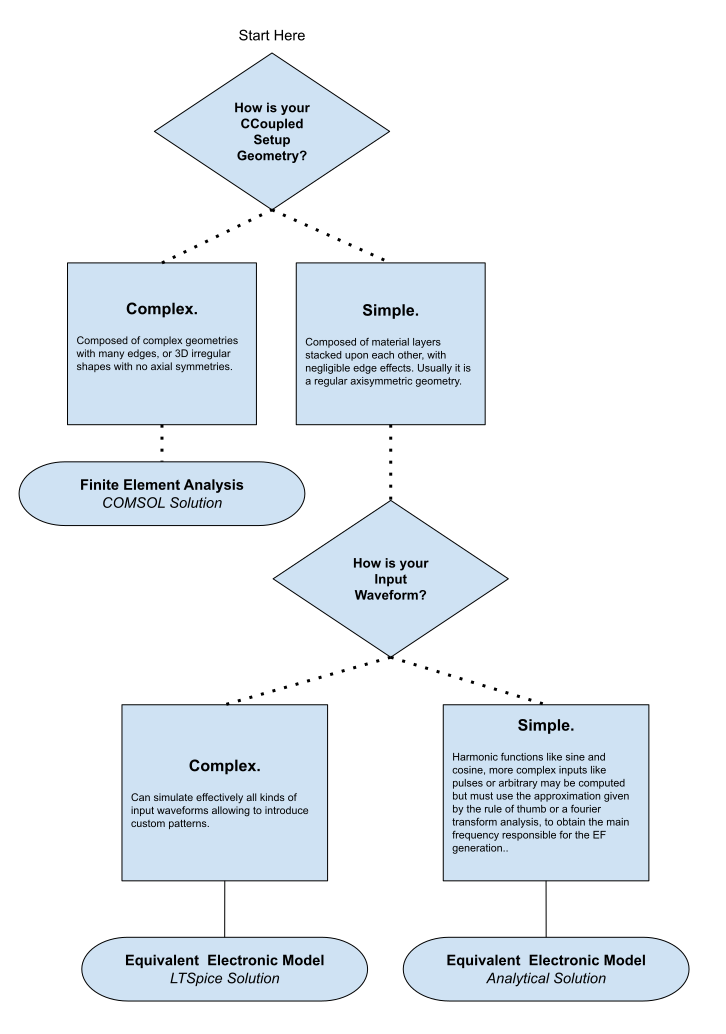
\includegraphics[scale=0.6]{./figures/Figure_5d10.png}}
\caption{Decision flowchart to choose an appropriate numerical modelling approach for a particular CCoupled setup.}
\label{fig5d10}
\end{figure}

If the geometry of the setup differs significantly from the ideal coaxial geometry of the constant section that is assumed in the analytical solution, then the \acs{FEM} method may be used to take into account the complexity of the geometry. However, even in the case of the geometry implemented in Rodan \textit{et al.} \cite{Rodan1978-yu} and shown in Figure \ref{fig5d7}a, it was possible to estimate the \acs{EF} using a simple cylindrical (coaxial) model (Figure \ref{fig5d7}b) and still obtain almost identical values for the \acs{EF} (Table \ref{tab_disagree}). Another advantage of the \acs{FEM} model is that it makes no assumptions about the frequency spectrum of the applied voltage, which is not the case for the analytical and circuit simulator approaches. Nonetheless, our predictions of the \acs{EF} for the eight studies analyzed (Tables \ref{tab_agree} and \ref{tab_disagree}) are practically the same for all three independent approaches (less than 3\% deviation from the mean value between the three prediction methods). 

The \acs{EF} values reported in the selected studies ranged from \num{1.0d-5} \si{\volt\per\meter} to \num{1.0d5} \si{\volt\per\meter}. According to our calculations, the actual range of applied fields was \num{1.0d-8} \si{\volt\per\meter} to \num{1.0d2} \si{\volt\per\meter}, still a range of 10 orders of magnitude. This is explained in part by the wide range of frequencies used, from Hz to MHz, and the fact that \acs{EF} strength is proportional to frequency in the setups described.

The effect of electrical stimulation on cell response is likely to be frequency-dependent. For example, Brighton \textit{et al.} \cite{Brighton1992-gg} failed to reproduce the effects on cell proliferation reported in Fitzsimmons \textit{et al.} \cite{Fitzsimmons1986-ks} at 10 \si{\hertz} and an \acs{EF} strength of \num{1.0d-5} \si{\volt\per\meter} (and note that Fitzsimmons probably applied a field 30 times weaker). On the other hand, Krueger \textit{et al.} \cite{Krueger2019-qk} have recently reported an effect on chondrocytic differentiation capacity with fields of \num{5.2d-6} \si{\volt\per\meter} and \num{5.2d-5} \si{\volt\per\meter} at a frequency of 1 \si{\kilo\hertz}. Thus, optimization of \acs{CCoupled} electrical stimulation protocols should consider E-Field strength and frequency as independent parameters.

Overall, the results presented in Tables \ref{tab_agree} and \ref{tab_disagree} show that the analytical and circuit simulator approaches outlined previously may give an estimate of the \acs{EF} intensity with sufficient accuracy for most purposes. We have assumed an homogeneous culture medium. But as previously shown, the presence of a scaffold can introduce local variations of the \acs{EF} (hotspots, coldspots) that may introduce localized effects on the cell culture \cite{Meneses2021-nd}. In this case, the \acs{FEM} approach should be applied to take into consideration the complex geometry of the scaffold.

We also analyzed the \acs{EF} in eight CCoupled setups that were used in twenty studies, published between 1978 and 2021. The \acs{EF} was correctly estimated in only 3 out of 8 setups and 8 out of 20 studies. We limited our analysis to bone and osteogenesis-related studies, but similar trends will probably be found in applications involving other tissues. The methods outlined here can be used to predict the \acs{EF} in CCoupled setups for electric stimulation of cell cultures of any type.     

Based on the analytical approach presented in this work, we have developed an \acs{EF} Calculator for \acs{CCoupled} systems with a layered cylindrical geometry (see Figure \ref{fig5d11}). This calculator is free, open-source, and publicly available for download from the Zenodo platform.\footnote{Developed CCoupled E-Field Calculator: https://doi.org/10.5281/zenodo.5897226} More details about the \acs{EF} calculator and its operation can be found in the original manuscript \cite{Meneses2022-yk}.

\begin{figure}
\makebox[\textwidth][c]{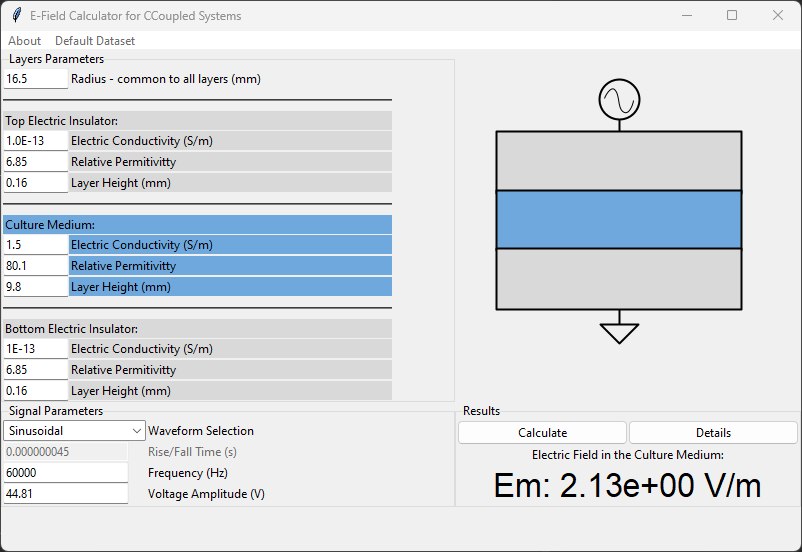
\includegraphics[scale=0.8]{./figures/Figure_5d11.png}}
\caption{Printscreen of the developed \acs{CCoupled} calculator graphical user interface displaying the magnitude of the \acs{EF} in the culture medium in the bottom right-hand corner for the setup reported in Brighton \textit{et al.}, 1992.}
\label{fig5d11}
\end{figure}  

Even though the laws of physics enable a reasonably accurate prediction of the \acs{EF} in the culture medium, the model should still be validated experimentally. Ideally, the \acs{EF} strength in the culture medium should be measured, but it may be difficult to do it correctly and accurately in most setups. Alternatively, the applied voltage and the current through the setup should be measured and reported. The ratio of these two quantities gives the total impedance of the setup, which can be compared with the value predicted by the model.

 

\section{Summary}

This chapter concluded that the effect of scaffold insertion on the \acs{EF} in the surrounding culture medium was mainly determined by the difference in electrical conductivity of these two materials (at low-frequency signals). The numerical simulations pointed to significant variations in local \acs{EF} patterns, which could lead to different cellular outcomes and confound the interpretation of the experimental results. According to the predictions, the presence of a scaffold can profoundly influence the \acs{EF} spatial patterns in its local environment by introducing local peaks and troughs or completely shielding the effects of external stimulation. The predicted \acs{EF} strongly depends on the electrical properties of the selected scaffold and culture medium. 

Also, this chapter showed a predominant overestimation of the \acs{EF} applied in reported \acs{CCoupled} stimulation studies. We analyzed eight CCoupled studies and sought to corroborate the reported estimates of the \acs{EF} in the culture medium. First, we reviewed the fundamental physics underlying \acs{CCoupled} stimulation and delineated three approaches to estimate the \acs{EF}. Using these approaches, we found that the reported values were overestimated in five studies, four based on incorrect assumptions. In all studies, insufficient information was provided to reproduce the setup exactly. Creating numerical models of experimental stimulation setups should improve the accuracy of the \acs{EF} estimates and enhance reproducibility. For this purpose, we developed a free, open-source tool, the \acs{EF} Calculator for \acs{CCoupled} systems, which is available for download from a public internet hosting platform.

At this point, the knowledge gathered in modelling different stimulation protocols, from mechanic stimulation due to fluid perfusion to \acs{EF} stimulation generated by \acs{DCoupled} or \acs{CCoupled} setups, was merged into the methodology of designing and constructing a singular bioreactor solution, which will be presented in the following chapter. 

%\newpage
%\bibliography{library_c5b} 
%\bibliographystyle{plain}
%\end{document}
%\documentclass[11pt]{report}
%\usepackage{siunitx}
%\usepackage{graphicx}
%\usepackage{makecell}
%\usepackage{booktabs}
%\usepackage[table,xcdraw]{xcolor}
%
%\begin{document}
%\setcounter{chapter}{5}
%\tableofcontents


\newpage
\chapter{Development of a novel bioreactor methodology: \textit{JANUS}}
This chapter explains the development of a novel bioreactor under an introduced methodology driven by numerical predictions. The resultant bioreactor was codenamed JANUS, which refers to the Roman god that represented a duality, here meaning a simultaneous physical and digital entity. The developed concept allows it to be easily fabricated with low-cost 3D printing, while simultaneously allowing the construction of precise microenvironment numerical models, unlocking predictions of important cell culture parameters for enhanced control and actuation. The created bioreactor concept is open source, highly replicable, and available to other research groups. This chapter traces the history behind this development. Its contents were collected from the following works:
\begin{itemize}
\item \small \textit{João Meneses, João C Silva, Sofia R Fernandes, Abhishek Datta, Frederico Castelo Ferreira, Carla Moura, Sandra Amado, Nuno Alves, and Paula Pascoal-Faria. 2020. “A Multimodal Stimulation Cell Culture Bioreactor for Tissue Engineering: A Numerical Modelling Approach.” Polymers 12 (4).};
\item \small \textit{João Meneses, Sofia R Fernandes, João C Silva, Frederico Castelo Ferreira, Nuno Alves and Paula Pascoal-Faria. 2023. ''JANUS: an open-source 3D printable perfusion bioreactor and numerical model-based design strategy for tissue engineering''. Front. Bioeng. Biotechnol. 11:1308096.};
\end{itemize}
This chapter's required cell culture procedures were made in collaboration with the SCERG - Stem Cell Engineering Research Group from iBB/IST - Instituto Superior Técnico, Portugal.
\newpage 




\section{Introduction}
Bioreactors for \textit{in vitro} cultures are increasingly used in \acs{TE} due to more complex mass transport requirements of growing tissues, and also to allow controlled reproduction of specific cellular environments that can promote particular cellular processes by applying stimulation (e.g., mechanical, electrical). Understanding the microenvironment generated by bioreactors is crucial to predict cell survival and fate in TE strategies \cite{Reina-Romo2019-ry}. \textit{In silico} models have been successfully applied to guide the development and optimization steps towards a bioreactor design that favors the best cellular outcomes regarding seeding, proliferation, and differentiation \cite{Engel2021-fk, Spencer2013-pg, Perier-Metz2021-bj}. Growing evidence reports multiple important environmental properties, like dissolved oxygen tension, glucose and lactate concentrations, and local pH value, that can strongly impact stem cell fate. They should be closely monitored and controlled \cite{Klein2021-dz, Klein2022-yj, Monfoulet2014-ef, Seddiqi2020-uo, Beskardes2018-fq}, regardless of how difficult and time/resource consuming can be to monitor and control specific cell microenvironments simultaneously. Predictions from computational studies help to determine the most relevant factors in the evolution and dynamics of biological systems \cite{Geris2018-tz}, optimizing control and modulation of cell cultures in bioreactor systems in a low-cost virtual environment.

Many bioreactor designs have been proposed in \acs{TE} to support better the proliferation and differentiation of several cell populations \cite{Smith2018-he, Montorsi2022-qm}. Some bioreactors include a specific set of sensors to allow improved monitorization of the \textit{in vitro} environmental conditions or actuator systems to apply different types of physical stimuli to promote cell differentiation (e.g., electric field, magnetic field, mechanical stress) \cite{Lim2022-dr}. Even if proven effective, most of these designs are not shared open-source with proper fabrication and integration instructions, which hinders reproducibility and usage by the \acs{TE} research community. The global massification of \acs{3D} printing technologies unlocks the opportunity to construct complex perfusion structures in suitable materials and techniques, while retaining high customization freedom, reproducibility, and shareability at a low cost \cite{Gensler2020-in, Haleem2020-oj}.

The considered workflow for developing a bioreactor consists of a series of interchained steps, as shown in Figure \ref{figWorkflow}. The first considered stage focused on the pre-design validation of construction materials and methods (spanning \acs{3D} printing technologies), including, if required, any material post-processing after fabrication. This stage of work was published in MDPI Polymers Journal under the title: "A Multimodal Stimulation Cell Culture Bioreactor for Tissue Engineering: A Numerical Modelling Approach" \cite{Meneses2020-dx}, presenting one of the first attempts to create a multimodal (mechanical and electric stimulation) perfusion bioreactor design along with its numerical models.

\begin{figure}
\makebox[\textwidth][c]{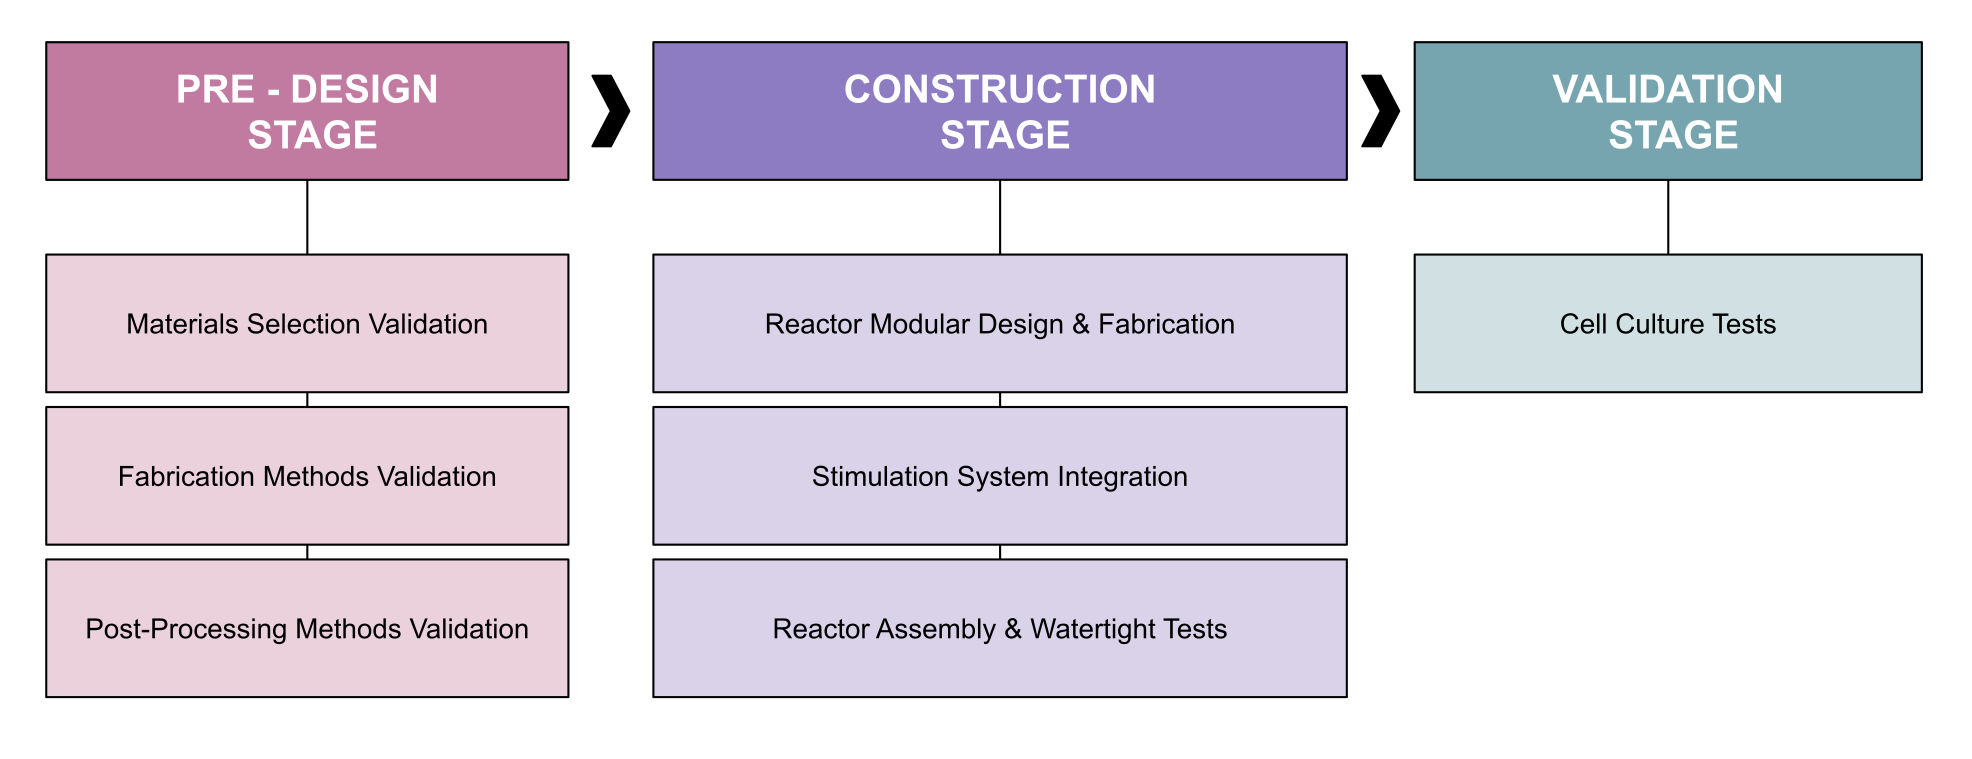
\includegraphics[scale=0.6]{figures/Figure_6d1}}
\caption{Workflow steps planned for the \textit{JANUS} bioreactor development, grouped by stages.}
\label{figWorkflow}
\end{figure}   

Recently we published the progress made in the construction and validation stages. A strategy was envisioned to iteratively design a perfusion bioreactor system based on model-driven decisions made on the microenvironment generated by each design hypothesis.  These decisions aim to obtain cell culture conditions that promote a particular cell line's high proliferation and differentiation rates (e.g., mesenchymal stem/stromal cells \cite{Bianconi2023-rs, Alvarez-Barreto2011-lj}, embryonic stem cells \cite{Marolt2012-xc}, induced pluripotent stem cells \cite{De_Peppo2013-dq}). Perfusion technology was selected due to its natural double role in bioreactor systems allowing the renovation of the culture medium and, at the same time, applying fluid flow-induced wall shear stress stimuli to the tissue constructs, which has been shown to enhance MSC-mediated bone formation \textit{in vitro} \cite{Wittkowske2016-xr, Schroder2022-qt, Yamada2022-aq}. For each microenvironment, \acs{FEM} models were used to predict the volumetric distributions of fluid flow-induced shear stress and \acs{EF} magnitude in culture regions. The proposed perfusion bioreactor system can be fabricated with \acs{3D} printing technologies (e.g., fused filament fabrication, stereolithography) and accommodates the capability for simultaneous electrical and mechanical stimulation of four scaffolds in identical conditions. The journey pursued to get the proposed bioreactor design is presented, from early conceptualization to the current version, following a multiple trial and error approach. The strategy of early integrating numerical models of the bioreactor-generated microenvironment into the design phase allows trying different stimulation protocols and geometric options before fabrication, saving time and reducing operational costs. After fabrication, we experimentally validated the bioreactor system outputs against their numerical model outputs to increase the confidence in the developed strategy, obtaining a digital twin of the experimental setup capable of improving environmental control of cell cultures and, at the same time, capable of providing a framework to study the cellular effects of the applied stimuli. The complete developed solution, including all bioreactors' components and numerical models, was named JANUS. This Roman inspiration describes here a duality of physical and virtual representations. JANUS is available in an online repository (https://doi.org/10.5281/zenodo.7695700, released under an open-source Attribution-ShareAlike 4.0 International license). JANUS approach can be potentially applied to any cell culture study in the context of \acs{TE} without any loss of applicability. Nevertheless, to establish design goals and allow \textit{in vitro} validation, we directed the current development to \acs{BTE} using a specific bone cell line since it constitutes an active research topic and a necessity to progress the understanding in this TE field of research \cite{Sladkova2014-yw}. The presented bioreactor development was motivated by successive approaches to deliver adequate in vitro mechanical and electrical stimulation conditions to bone cells seeded on 3D-printed porous PCL scaffolds, in order to generate an osteogenic stimulation protocol that may mimic the native human bone microenvironment, and consequently, improve the regenerative outcomes.

\begin{figure}
\makebox[\textwidth][c]{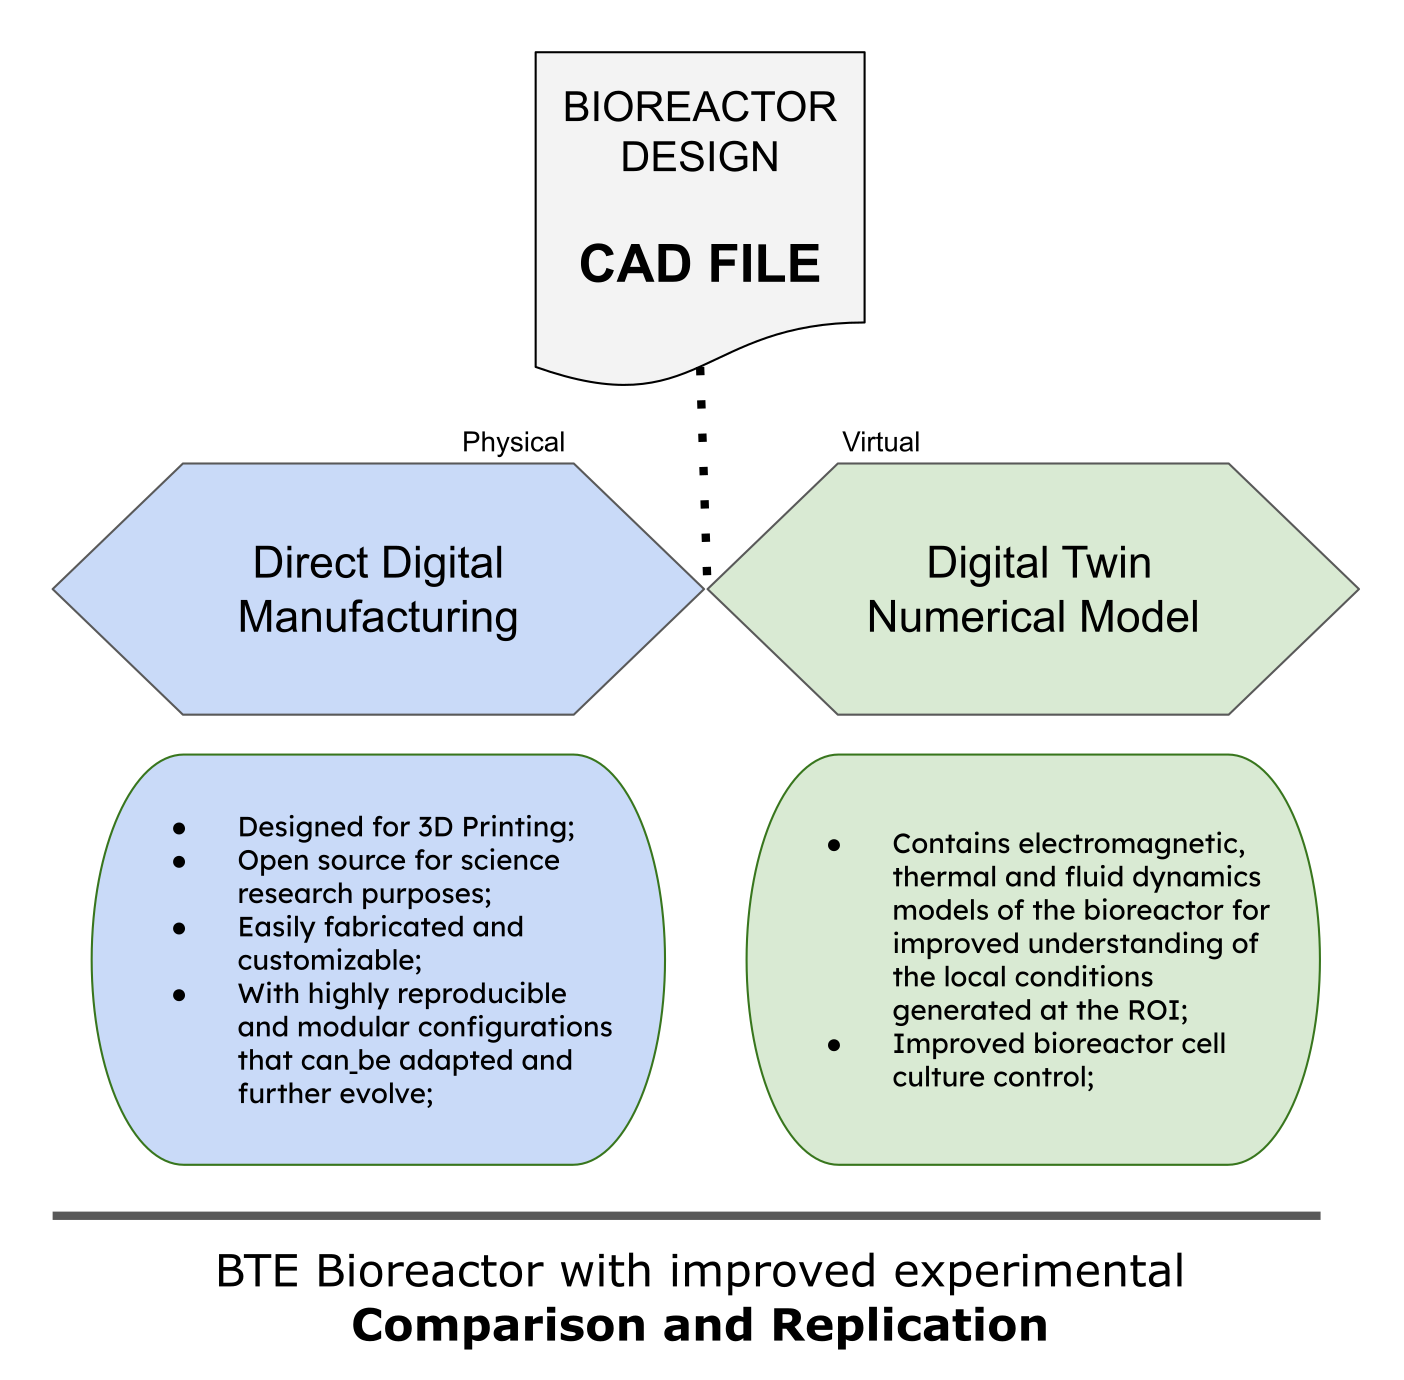
\includegraphics[scale=0.6]{./figures/Figure_6d2}}
\caption{The JANUS bioreactor duality concept based in a shared root \acs{CAD} file, using this standard file to create detailed methodologies for physical and virtual replication.}
\label{figCadFile}
\end{figure}  

The proposed JANUS bioreactor duality (physical and virtual entity) concept is built on top of a geometrical design \acs{CAD} file, see Figure \ref{figCadFile}. With this file, all structures, components, and parts of the bioreactor (including any existing scaffold structure) could be geometrically represented with accurate dimensions and in their experimental position. The \acs{CAD} file can easily be shared among scientists to be used in two ways: first, to replicate the bioreactor concept through additive and/or subtractive construction methods (assuming that all construction methodologies are also shared with sufficient detail); second, to run bioreactor numerical models based on \acs{FEM} analysis, allowing to predict, test and optimize physical/chemical microenvironments. This combination of capabilities allows for continuously improved bioreactor design and control of generated environments, impacting experimental replicability.




\section{Aim}
\begin{itemize}
\item Validate an adequate biocompatible material after being produced by additive manufacturing method and post-processed to fabricate a bioreactor part; 
\item Design a multimodal stimulation perfusion bioreactor based on numerically model-driven decisions made on the microenvironment generated by each design hypothesis;
\item With the designed bioreactor \acs{CAD} file, fabricate the physical bioreactor with \acs{3D} printing technologies and simultaneously create the bioreactor digital model;
\item Validate the fabricated bioreactor design, confirming its stimulation outputs against their corresponding numerical models. Run preliminary \textit{in vitro} cell culture tests.
\end{itemize}




\section{Methods}


\subsection{Material samples production}
This process goal was to simultaneously validate an adequate biocompatible material, additive manufacturing method, and post-processing steps to fabricate a bioreactor. To do so, simple parallelepiped samples with dimensions of 10 \si{\milli\meter} of depth, 10 \si{\milli\meter} of width and 5 \si{\milli\meter} of height were drawn in SOLIDWORKS 2018 Student Edition (Dassault Sistèmes), and then exported to the stereolithography file format (*.stl). This file was then imported to each additive manufacturing technology native software as described in Table \ref{tabMat}. All samples from the same material were printed under the same conditions. Table \ref{tabMat} summarises the type and additive manufacturing methodology for each material sample fabricated. Materials used were selected based on additive manufacturing compatibility, suitable mechanical properties, cost, easy processing, and material transparency. The latter feature may play a key role in real-time visualization of the scaffold during \textit{in vitro} bioreactor cultures.   
 
\begin{table}
\caption{Description of tested samples identity (ID), material, correspondent supplier, and additive manufacturing methodology.}
\bigskip
\tiny
\centering
\begin{tabularx}{325px}{c c l l} \toprule[0.15em]
\textbf{Sample ID}	& \textbf{Material}	& \textbf{Supplier} & \textbf{AM Methodology}\\ \cmidrule(l){1-4}

PCL & Polycaprolactone 
& \makecell[l]{FACILAN™ PCL 100,\\ 750 GRAM (MW: 50000 g/mol),\\ 1.75 MM,\\ 3D4MAKERS,\\ Haarlem, The Netherlands}
& \makecell[l]{
3DP Technology: FDM;\\
3D Printer: Creatbot F430;\\
Nozzle Diameter: 0.4 \si{\milli\meter};\\
Nozzle Temperature: 165 \si{\celsius};\\
Heated Bed Temperature: 35 \si{\celsius};\\
Chamber Temperature: 20 \si{\celsius};\\
Printing Speed: 60 \si{\milli\meter\per\second};\\
Infil: 100 \si{\percent}.}
\\ \cmidrule(l){1-4}
PA			
& Polyamide/Nylon			
& \makecell*[l]{PA Powder,\\ 3D SYSTEMS}		
& \makecell*[l]{3DP Technology: SLS;\\
3D Printer: 3D System sPro 60 HD-HS;\\
CO2 Laser 70 \si{\watt};\\
Layer Thickness:  0.1 \si{\milli\meter};\\
Scanning Speed: 6 \si{\meter\per\second};\\
Construction Chamber Temperature: 173 \si{\celsius};\\
Feeding Chamber Temperature: 135 \si{\celsius}.}
\\ \cmidrule(l){1-4}
PETG			
& \makecell{Polyethylene\\ Terephthalate\\ Glycol-modified}
& \makecell[l]{PETG FILAMENT,\\ 750 GRAM,\\ 1.75MM,\\ 3D4MAKERS,\\ Haarlem, The Netherlands}
& \makecell[l]{
3DP Technology: FDM;\\
3D Printer: Creatbot F430;\\
Nozzle Diameter: 0.4 \si{\milli\meter};\\
Nozzle Temperature: 260 \si{\celsius};\\
Heated Bed Temperature: 110 \si{\celsius};\\
Chamber Temperature: 60 \si{\celsius};\\
Printing Speed: 60 \si{\milli\meter\per\second};\\
Infil: 100 \si{\percent}.}
\\ \cmidrule(l){1-4}
ABS		
& \makecell{Acrylonitrile-\\Butadiene-\\Styrene}
& \makecell[l]{ABS FILAMENT,\\ 750 GRAM,\\ 1.75MM,\\ 3D4MAKERS, Haarlem,\\ The Netherlands}
& \makecell[l]{
3DP Technology: FDM;\\
3D Printer: Creatbot F430;\\
Nozzle Diameter: 0.4 \si{\milli\meter};\\
Nozzle Temperature: 230 \si{\celsius};\\
Heated Bed Temperature: 50 \si{\celsius};\\
Chamber Temperature: 35 \si{\celsius};\\
Printing Speed: 60 \si{\milli\meter\per\second};\\
Infil: 100 \si{\percent}.}
\\ \cmidrule(l){1-4}
C8		
& \makecell{Proprietary Polymer\\ Composite produced\\ by ELOGIOAM 3D\\ MATERIALS}
& \makecell[l]{FACILAN™ C8 FILAMENT,\\ 750 GRAM,\\ 1.75MM,\\ 3D4MAKERS, Haarlem,\\ The Netherlands}
& \makecell[l]{
3DP Technology: FDM;\\
3D Printer: Creatbot F430;\\
Nozzle Diameter: 0.4 \si{\milli\meter};\\
Nozzle Temperature: 195 \si{\celsius};\\
Heated Bed Temperature: 35 \si{\celsius};\\
Chamber Temperature: 20 \si{\celsius};\\
Printing Speed: 60 \si{\milli\meter\per\second};\\
Infil: 100 \si{\percent}.}
\\ \cmidrule(l){1-4}
PPSU		
& \makecell{Polyphenylsulfone}
& \makecell[l]{PPSU FILAMENT,\\ 500 GRAM,\\ 1.75 MM,\\ 3D4MAKERS, Haarlem,\\ The Netherlands}
& \makecell[l]{
3DP Technology: FDM;\\
3D Printer: Creatbot F430;\\
Nozzle Diameter: 0.4 \si{\milli\meter};\\
Nozzle Temperature: 380 \si{\celsius};\\
Heated Bed Temperature: 120 \si{\celsius};\\
Chamber Temperature: 60 \si{\celsius};\\
Printing Speed: 60 \si{\milli\meter\per\second};\\
Infil: 100 \si{\percent}.}
\\ \cmidrule(l){1-4}
PEEK		
& \makecell{Polyether\\ Ether\\ Ketone}
& \makecell[l]{PEEK FILAMENT,\\ 500 GRAM,\\ 1.75 MM,\\ 3D4MAKERS, Haarlem,\\ The Netherlands}
& \makecell[l]{
3DP Technology: FDM;\\
3D Printer: Creatbot F430;\\
Nozzle Diameter: 0.4 \si{\milli\meter};\\
Nozzle Temperature: 390 \si{\celsius};\\
Heated Bed Temperature: 120 \si{\celsius};\\
Chamber Temperature: 60 \si{\celsius};\\
Printing Speed: 60 \si{\milli\meter\per\second};\\
Infill: 100 \si{\percent}.}
\\ \bottomrule[0.15em]
\end{tabularx}
\label{tabMat}
\end{table}


\subsection{\textit{In vitro} cytotoxicity tests}
The biocompatibility of the different materials considered for the bioreactor fabrication was assessed using L929 mouse fibroblasts (ATCC number CCL-1) and following the ISO 10993-5 and ISO 10993-12 guidelines \cite{For_Standardization2009-wo}. Before the test, the materials were sterilized by ultraviolet exposure overnight, ethanol 70\si{\percent} washing and incubation with a 1\si{\percent} antibiotic--antimycotic (Anti--Anti, Gibco\texttrademark, Fisher Scientific, USA) solution in phosphate-buffered saline (PBS, Gibco\texttrademark, Fisher Scientific, USA). All materials were evaluated by performing the indirect extract test and direct contact test. L929 fibroblasts were cultured on tissue culture polystyrene plates with Dulbecco’s Modified Eagle’s Medium (DMEM, Gibco\texttrademark, Fisher Scientific, USA) supplemented with 10\si{\percent} (\emph{v}/\emph{v}) Fetal Bovine Serum (FBS, LifeTechnologies, USA) and with 1 \si{\percent} Anti--Anti in an incubator at 37 \si{\celsius}/5 \si{\percent} CO$_{2}$, to be used as a negative control. Latex was used as a positive control for cell death. Extracts were prepared by incubating the materials in DMEM + 10 \si{\percent} FBS + 1 \si{\percent} Anti--Anti culture media at a ratio of 0.2 \si{\gram} of material/\si{\milli\liter} for 72 \si{\hour} at 37 \si{\celsius}/ 5 \si{\percent} CO$_{2}$. This ratio ensures that the test sample covers one-tenth of the cell layer surface, according to the ISO 10993-5:2009 \cite{For_Standardization2009-wo}. L929 fibroblasts were seeded on tissue culture polystyrene plates at a cell density of 10$^{5}$ cells per well and cultured for 24 \si{\hour} at 37\si{\celsius}/ 5\si{\percent} CO$_{2}$ to generate a confluent monolayer. For the indirect extract test, the culture media was removed, and L929 cells were exposed to the material extract’s conditioned medium for 72 \si{\hour} at 37\si{\celsius}/ 5\si{\percent} CO$_{2}$. Then, extract conditioned media were removed, and the MTT (3-(4,5-dimethylthiazol-2-yl)-2-5 diphenyl tetrazolium bromide) assay (In Vitro Toxicology Assay Kit MTT based, Sigma-Aldrich, USA) was performed by the manufacturer’s guidelines. Briefly, cells were incubated with MTT solution (1 mg/mL, yellow) for 2\si{\hour} at 37\si{\celsius}. Afterward, the violet formazan product resultant from the MTT metabolic reduction by metabolically active cells was dissolved under agitation using a 0.1 \si{\molar} HCl solution in anhydrous isopropanol (Sigma-Aldrich). Absorbance values of the resultant solutions were measured in a plate reader (Infinite M200 PRO, TECAN, Mannedorf, Switzerland) at 570 \si{\nano\meter}. The direct contact assay was performed by the ISO standards mentioned above. Individual specimens of the test samples were carefully placed over previously formed confluent monolayer of L929 fibroblasts (in the center of each of the replicate wells; three replicates were used for each sample). The materials were in direct contact with the L929 cell monolayer, incubated for 72\si{\hour} at 37\si{\celsius}/ 5\si{\percent} CO$_{2}$, according to the ISO 10993-5:2009 standard. Afterward, cell viability and morphology were evaluated qualitatively under an inverted optical microscope (LEICA DMI3000B, Leica Microsystems, Wetzlar, Germany) equipped with a digital camera (Nikon DXM1200F, Nikon Instruments Inc., Melville, USA) to assess any cytotoxic responses such as the occurrence of halo inhibition effect or abnormal cell morphology.


\subsection{Bioreactor design based on model-driven decisions}
A bottom-top approach to bioreactor design was guided by \acs{FEM} based models. The decision tree applied for the bioreactor development is described in this section in a step-by-step manner (Figure \ref{figStrategy}). A cyclic iteration between \acs{CAD} design and \acs{FEM} predictions is conducted until the established microenvironment for that particular design is achieved. With this approach, we aim to reach a design that, once fabricated, can operate as numerically predicted. We only report here the fundamentals of every development step. A full description is reported in the original manuscript that originated this chapter, along with the complete roadmap of this bioreactor development. A glimpse of the evolution of this bioreactor design concept, main features, and subsequent methodology, defined in this thesis work, can be observed in Figure \ref{figStory}. To facilitate reproducibility, all systems developed in this work have only considered commercially available components or custom-made \acs{3D} printing parts.  

\begin{figure}
\makebox[\textwidth][c]{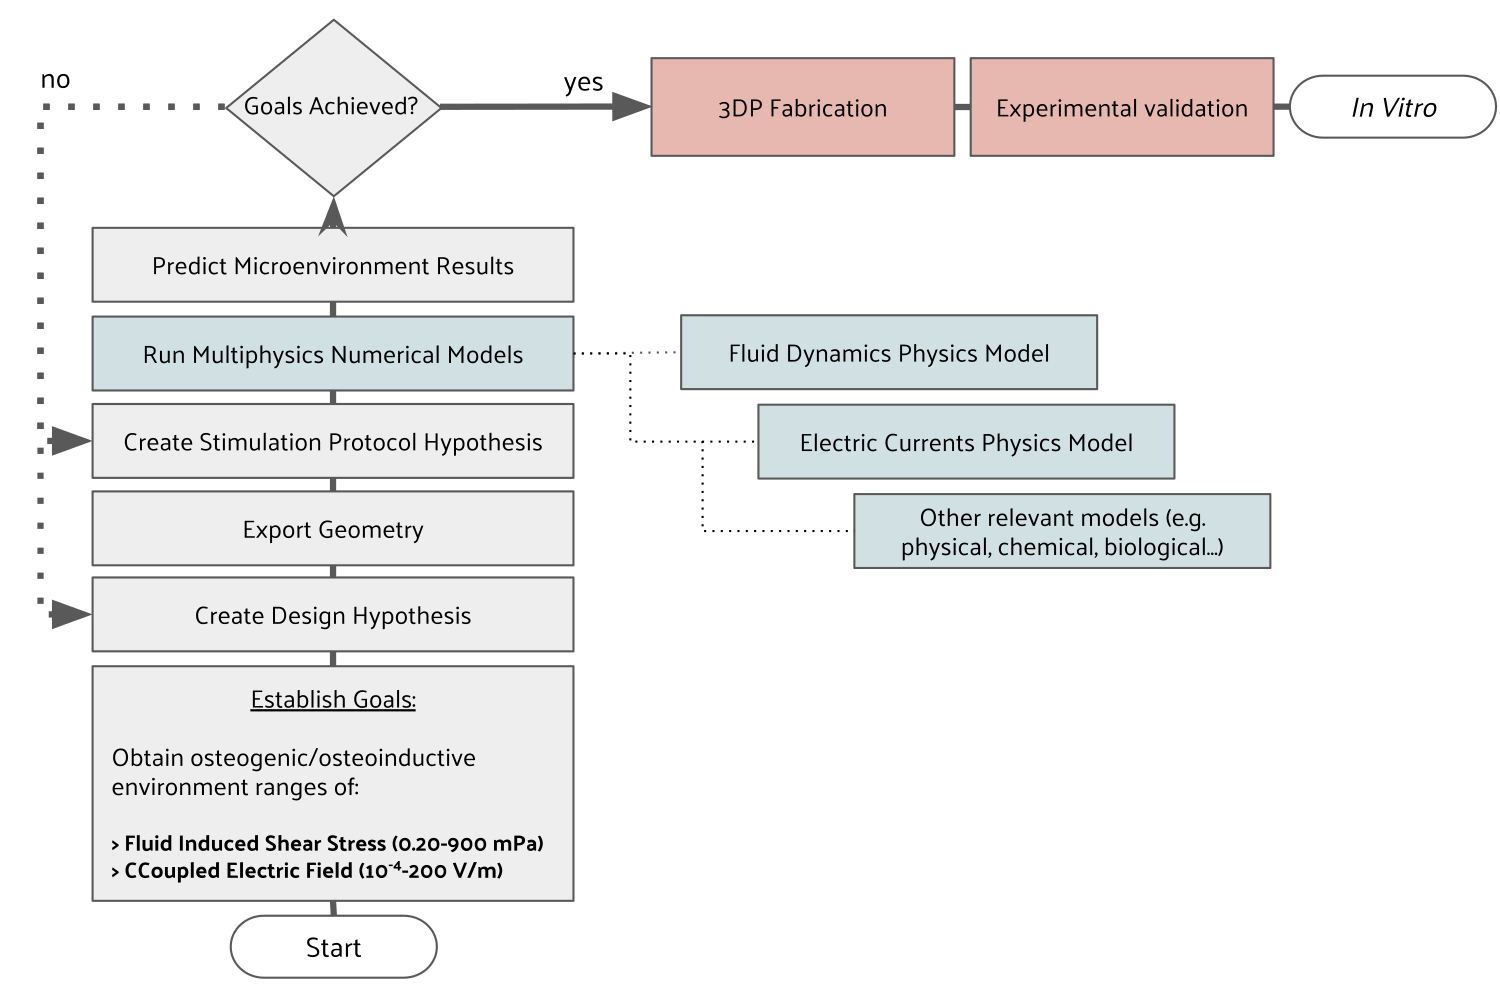
\includegraphics[scale=0.8]{./figures/Figure_6d4}}
\caption{Decision tree used to iterate between \acs{CAD} design and stimulation protocol hypotheses until \acs{FEM} predictions matched an intended microenvironment.}
\label{figStrategy}
\end{figure}

\begin{sidewaysfigure}
\makebox[\textwidth][c]{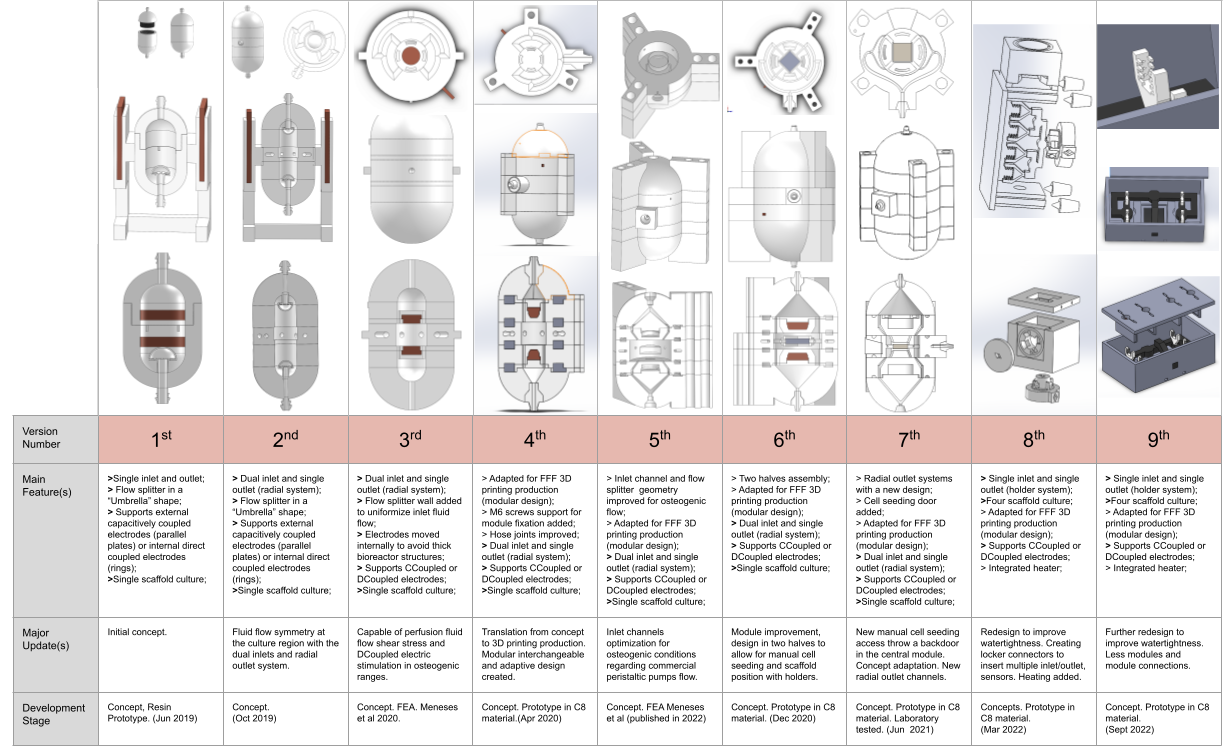
\includegraphics[scale=0.45]{./figures/Figure_6d4b}}
\caption{Development timeline of the bioreactor until the 9\textsuperscript{th} version used as the starting point for the bioreactor update presented in the current chapter.}
\label{figStory}
\end{sidewaysfigure}


\subsubsection{Defining the bioreactor system development goals}
The starting point for this design was a previously developed bioreactor concept \cite{Meneses2020-dx, Meneses2022-rx}. This design was progressively modified to integrate multiple actuators and sensors while preserving the ability to be entirely \acs{3D} printable (Figure \ref{figStory}). Culture medium volume usage was minimized, and sensor probes were included for online monitoring (e.g., pH, dissolved oxygen, temperature).

Perfusion bioreactors allow reaching cell-seeded scaffolds with homogeneous nutritional supply while removing waste products effectively, favoring appropriate cell metabolic activity \cite{Shakeel2013-vo, Gaspar2012-uz}. Also, the induced fluid flow shear stress can simultaneously act as a mechanical stimulus to promote improved responses in some cellular lines (bone cells included). Due to these two attributes, perfusion technology was selected for this development to ensure proper osteogenic conditions of the microenvironment. We chose a wall shear stress range in agreement with those previously observed to produce osteoinductive effects for mesenchymal stem/stromal cells. We refer to the osteoinductive ranges of 1.47-24 \unit{\milli\pascal} \cite{Vetsch2017-zd} and 0.20-13.35 \unit{\milli\pascal} \cite{Yamada2021-qf}. We emphasize that the resultant wall shear stress range is a product of the bioreactor-generated fluid flow characteristics, being also influenced by the scaffold properties, including its geometry and surface topology.

The other technical decision was to select adequate electrical stimulation technology for \textit{in vitro} cultures. Evidence of \acs{EF} technologies to support osteogenic processes has built up over the last decades and is extensively reviewed by Nicksic \textit{et al.} \cite{Nicksic2022-jy}. We decided on \acs{CCoupled} systems, since these ensure the delivery of a pure \acs{EF} stimulation without faradaic byproducts or an accompanying magnetic field. \acs{CCoupled} electrodes were fabricated from indium tin oxide coated polyethylene terephthalate (ITO PET) films (33x18 \unit{\milli\meter}), with a 175 \unit{\micro\meter}-thick polyester film coated with indium tin oxide (60 \unit{\ohm}/sq) that was glued with polydimethylsiloxane (PDMS) to a 3D printed structure. Regarding \acs{CCoupled} stimulation, the system will be designed to deliver an \acs{EF} with a wide range of magnitudes, considering the values previously reported of \num{1.0d-5} to \num{1.3d+3}\unit{\volt\per\meter} \cite{Fitzsimmons1986-ks, Korenstein1984-qb}, using a frequency of 60 \unit{\kilo\hertz} as applied by other previous \acs{CCoupled} works addressing bone regeneration \cite{Brighton1992-gg, Stephan2020-qh}.


\subsubsection{Creating geometrical design hypotheses}
All bioreactor and scaffold parts were designed with SOLIDWORKS (2018 Student Edition, Dassault Sistèmes), a parametric \acs{CAD} software. Two scaffold geometries were selected from the literature as an example to apply the described development methodology (Figure \ref{figParts}a, \ref{figParts}b). Our selection criteria were to consider scaffold geometries actively used in bone tissue engineering research, capable of matching the mechanical properties of cortical or trabecular bone formations to some extent. 

The first scaffold geometry selected is from Hayashi \textit{et al.} work \cite{Hayashi2019-qx, Hayashi2020-fr, Hayashi2022-oa, Shibahara2022-kj}, consisting of a honeycomb structure scaffold for bone regeneration, made from carbonate apatite to resemble natural human bone mineral composition. Their studies tested different macropore and micropore volumes, demonstrating that high interconnectivity and uniformity of channels enable scaffolds to maintain high mechanical properties and osteogenic ability while being suitable to be applied as implants for weight-bearing areas \cite{Hayashi2019-qx, Hayashi2020-fr}. This honeycomb scaffold structure was produced by extrusion molding, with a reported Young’s moduli of 23 \unit{\giga\pascal} \cite{Hayashi2020-fr}, higher than the usual Young’s moduli value for cortical (18-21 \unit{\giga\pascal}) or trabecular (10-15 \unit{\giga\pascal}) bone formations \cite{Morgan2018-pv}, but with the potential to be tailored by porous structures design to mimic mechanical properties of bone structures. The \acs{CAD} geometry of the honeycomb structure scaffold was considered with an external envelope volume of 10.2x10.2x3.0 \unit{\milli\meter}, a truss size of 250 \unit{\micro\meter} and a macropore size of 300 \unit{\micro\meter}. 

The second scaffold geometry selected is a regular orthogonal scaffold that, when produced from ceramic materials, such as biphasic calcium phosphate \cite{Touri2018-jw} or lithium-calcium-silicate crystal \cite{Chen2019-ap}, has reported properties similar to native bone minerals. The \acs{CAD} geometry of the orthogonal scaffold presents an external envelope volume of 10.0x10.0x2.75 \unit{\milli\meter}, while maintaining the geometrical relations and dimensions reported by Touri \textit{et al.} \cite{Touri2018-jw}, with a filament diameter and pore size of 500 \unit{\micro\meter}. Due to typical 3D printing fabrication constraints and to ease numerical models, a filament superposition of 10 \% and round fillets of 0.02 \unit{\milli\meter} diameter were added to each orthogonal intersection.


\begin{figure}
\makebox[\textwidth][c]{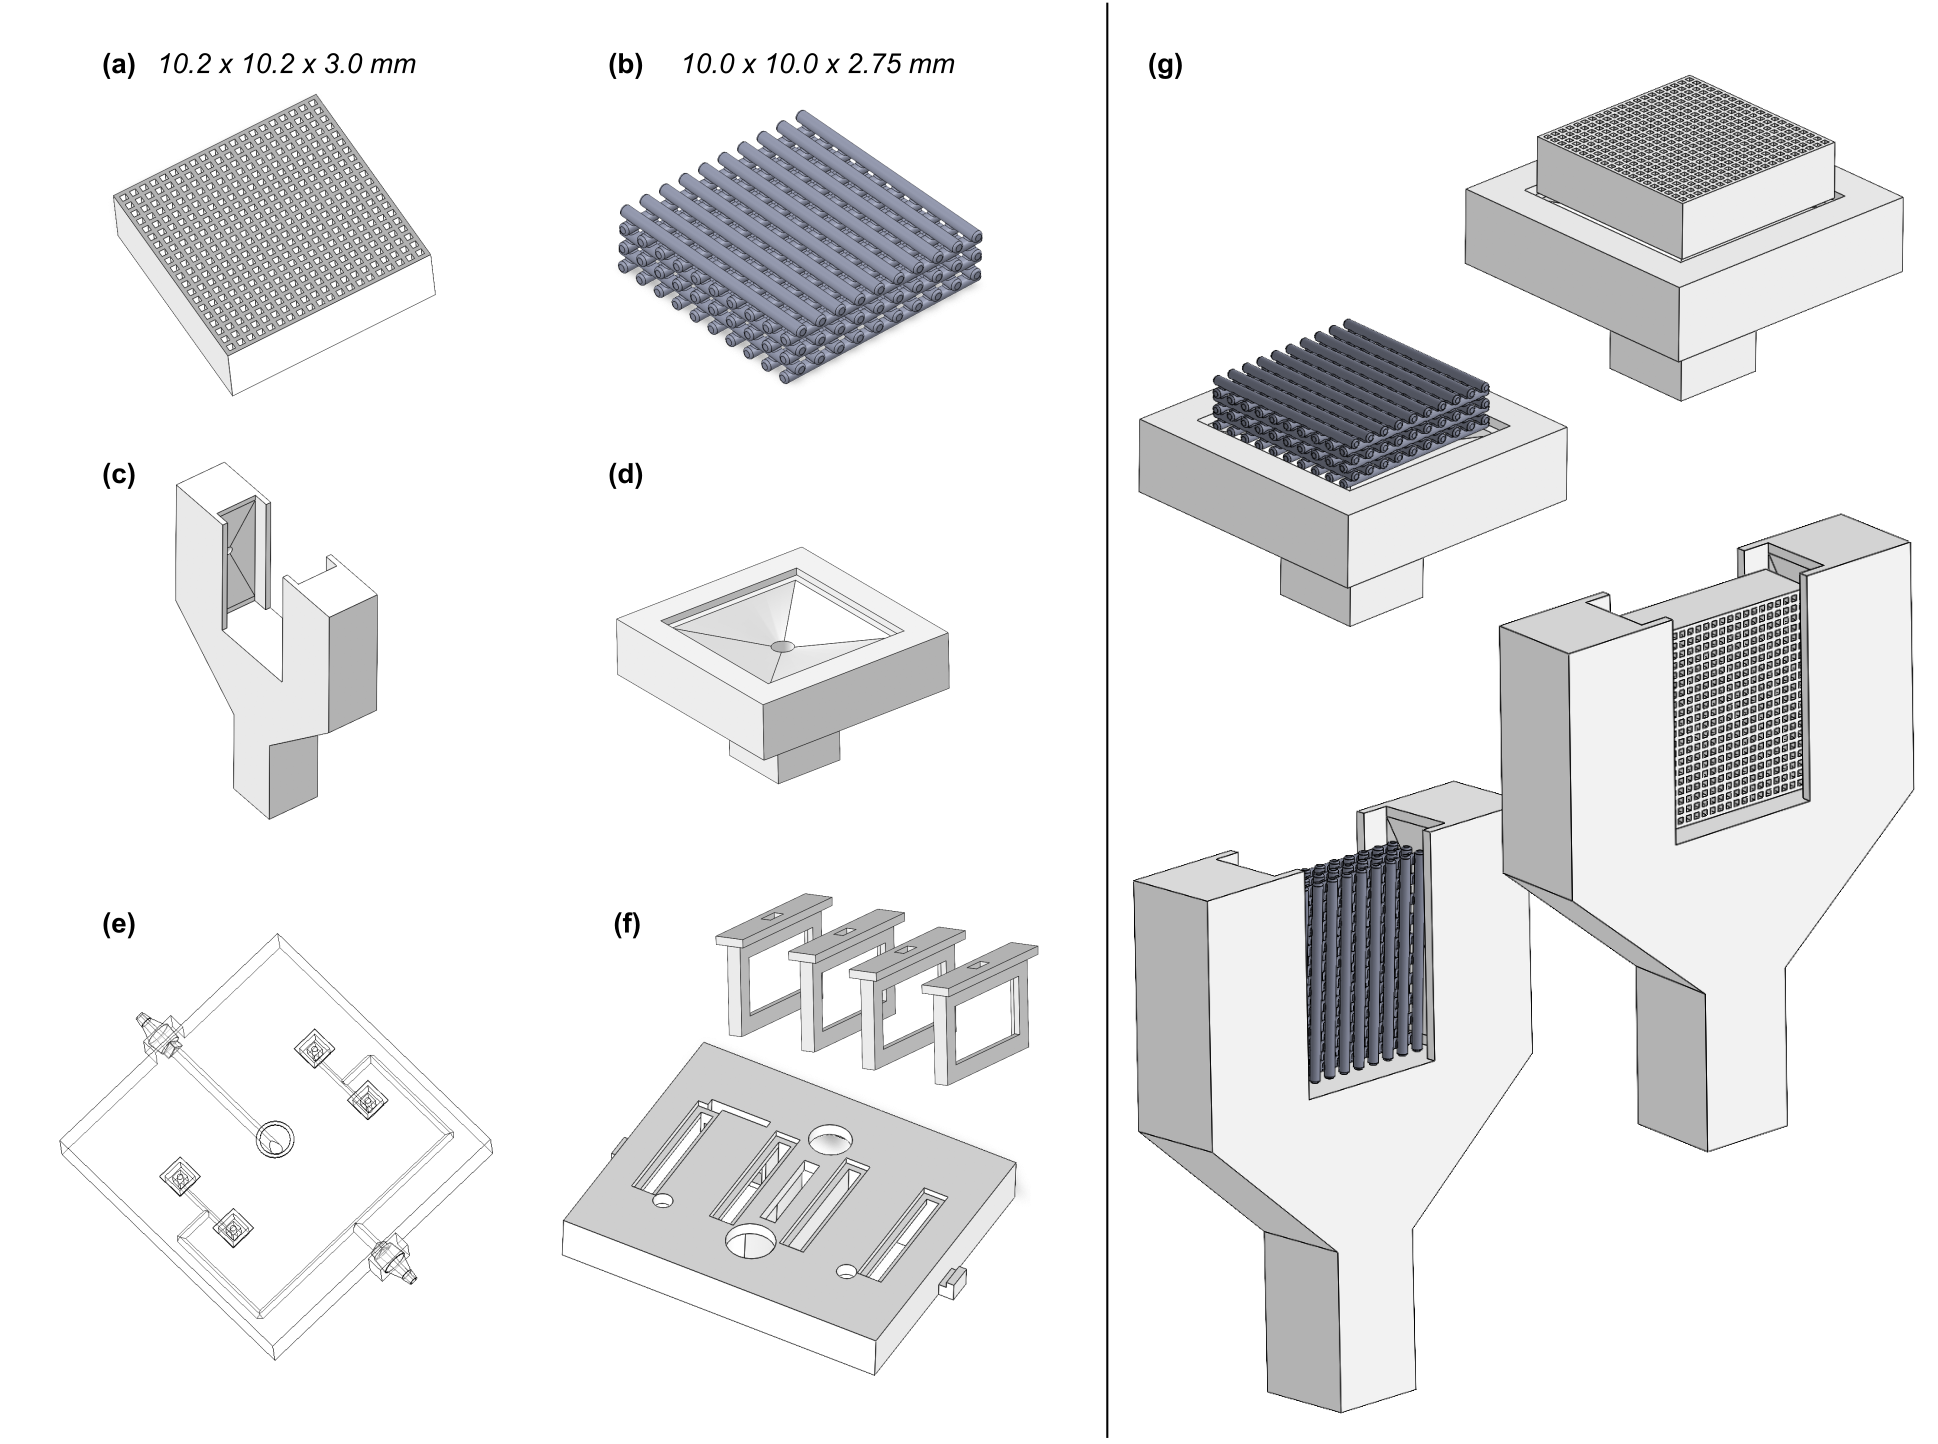
\includegraphics[scale=0.6]{./figures/Figure_6d5}}
\caption{Geometrical design hypotheses considered. (a) Honeycomb scaffold structure; (b) Orthogonal scaffold structure; (c) Vertical scaffold holder; (d) Horizontal scaffold holder; (e) Outlet channel network; (f) Support for CCoupled electrodes; (g) Combinations of scaffold and holder considered for simulations.}
\label{figParts}
\end{figure}


In addition to the scaffold design hypothesis, two versions of scaffold holders were conceived to provide support in different positions (vertical vs. horizontal), also incorporating different outlet flow channels (Figure \ref{figParts}c, \ref{figParts}d). The reason for this holder hypothesis was to provide different fluid flow characteristics (one bottom outlet vs. two lateral outlets), and also, since the CCoupled system is mounted laterally, the created holder hypothesis allows testing two electric stimulation configurations. To connect each of the bioreactor's four scaffold holders to the outlet peristaltic tube, a channel network (Figure \ref{figParts}e) was designed to guarantee that, at every channel split, the sum of section areas of the child branches is equal to the section area of the parent branch, condition necessary to minimize flow velocities loss, since it divides the outlet flow equally among all supported scaffolds. Regarding the \ac{CCoupled} system, since stimulation amplitude, waveform, and duration are the most determinant parameters for the \ac{CCoupled} effects, all geometrical variations of electrode number, position, or size were not considered in this work, being described elsewhere \cite{Tandon2008-jg}. Thus, the delivery range of the \acs{EF} in this work was varied only by changing the input waveform of the stimulation protocol. The electrodes for the \ac{CCoupled} system were placed in parallel positions and equidistant from the scaffold center, 22 \si{\milli\meter} apart, in such a way that each electrode pair will stimulate two side-by-side scaffolds (Figure \ref{figParts}f). 

The decision to have four scaffolds per bioreactor was to increase statistical power in the experimental condition, being a common practice in \acs{TE} to replicate the same condition in a high number of samples ($N>3$) \cite{Pollard2019-tz, Silva2020-dc}. To avoid unnecessary simulations and decrease computational effort, the proposed work was separated into two blocks: 1) obtain the outlet channel network design that minimizes the fluid flow velocity loss; 2) all combinations of scaffolds and holders designs were considered, resulting in four models that were analyzed with fluid flow and \acs{EF} simulation studies. The combination of geometries and protocol which predictably results in the closest conditions to an osteogenic microenvironment were selected for fabrication and validation.


\subsubsection{Setting simulation input parameters}
Each protocol was selected considering the maximum output of the available lab equipment (electric signal source and peristaltic pump), guaranteeing that the highest magnitudes possible for the available lab equipment were obtained for each stimulation condition at the cell culture chamber. Once determined the bioreactor-generated microenvironments for the maximum equipment's output, we established our working baseline: the peristaltic pump flow rate was set to the maximum continuous outlet flow of 50 \unit{\milli\liter\per\minute}, mounted with a 2.79 \unit{\milli\meter} internal diameter peristaltic tube (0.328 \si{\meter\per\second} at the peristaltic tube end); the CCoupled input waveform generator was set to its maximum amplitude of 10 \si{\volt}\textsubscript{p-p} for a sinusoidal wave with a frequency of 60 \unit{\kilo\hertz}. Both stimulation protocol parameters were considered as inputs for the developed numerical models.


\subsubsection{Multiphysics numerical simulations}
Each designed part was exported to the \acs{STEP} file format, allowing it to be imported and post-processed by COMSOL Multiphysics \acs{FEM} software (version 5.2a, www.comsol.com). Meshing was performed with the physics-controlled mesh and fine options. These options translated to meshes made from free tetrahedral elements with an average element quality of 0.68. Further mesh characterization data is available in the COMSOL reports, downloadable in an online repository (https://doi.org/10.5281/zenodo.7695700). Meshes were constructed with a high number of nodes to guarantee mesh-independent results (computable by the processor AMD Ryzen 7 5700G 8-Core 3.8GHz c/ Turbo 4.6GHz 20MB SktAM4). Two COMSOL physics interfaces were applied for each stimulation mode. For fluid flow shear stress calculations, \acs{CFD} stationary studies were conducted with the single phase Laminar Flow physics interface, which solves the Navier-Stokes equations for the conservation of momentum and the continuity equation for the conservation of mass. The cell culture medium was considered as an incompressible Newtonian fluid, with viscous material properties similar to water, as applied by Hidalgo-Bastida \textit{et al.} \cite{Hidalgo-Bastida2012-tp} and in our previous works \cite{Meneses2020-dx, Meneses2022-rx}. Outlet channel network flow models were imposed with an outlet velocity boundary condition of 0.328 \unit{\meter\per\second} applied to the peristaltic tube connector, and a standard atmosphere pressure (\num{1.01d5} \unit{\pascal}) inlet boundary condition applied to the scaffold holder connector channel. Flow models for scaffold and holder combinations were enclosed by a cylindrical volume with a radius of 20 \unit{\milli\meter} and a height of 30 \unit{\milli\meter} to represent a part of the culture medium domain inside the bioreactor chamber. The atmospheric pressure inlet boundary condition was considered in all surrounding cylindrical surfaces. In contrast, a single outlet boundary condition was added to the exit surface of the scaffold holder channel (designed with equal dimensions for both holder options). The scaffold holder outlet boundary condition was defined with the average velocity magnitude value (0.120 \unit{\meter\per\second}) obtained from the first outlet channel network model solution.


\begin{table}
\caption{Material properties for numerical model domains.}
\bigskip
\footnotesize
\centering
\begin{tabularx}{350px}{l l} \toprule[0.15em]
\textbf{Material} & \textbf{Properties} \\ \cmidrule(l){1-2}

Osteogenic Culture Medium (37  \unit{\celsius}) & 
\begin{tabular}[c]{@{}l@{}}Electric conductivity: 1.5 \unit{\siemens\per\meter} \\
Relative permittivity: 80.1 \\
Kinematic viscosity: \num{6.89d-4} \unit{\pascal\second} \\
Density: \num{9.94d2} \unit{\kilo\gram\per\cubic\meter} \cite{Gabetti2022-hp}
\end{tabular} \\ \cmidrule(l){1-2}

Electrode - ITO part                                                                   
& \begin{tabular}[c]{@{}l@{}}Electric Conductivity: \num{1.0d6} \unit{\siemens\per\meter} \\ 
Relative permittivity: 1 \cite{ReviewMIT}
\end{tabular} \\  \cmidrule(l){1-2}

Electrode - PET part 
& \begin{tabular}[c]{@{}l@{}}Electric Conductivity: \num{1.0d-21} \unit{\siemens\per\meter} \\
Relative permittivity: 3 \cite{ReviewMIT} 
\end{tabular} \\ \cmidrule(l){1-2}

C8 (PLA composite) - bioreactor parts
& \begin{tabular}[c]{@{}l@{}}Electric Conductivity: \num{1.0d-21} \unit{\siemens\per\meter} \\
Relative permittivity: 2.7 \cite{Hegde2015-nd}
\end{tabular} \\ \cmidrule(l){1-2}

PCL - scaffold 
& \begin{tabular}[c]{@{}l@{}}Electric Conductivity: \num{1.0d-13} \unit{\siemens\per\meter}\\ 
Relative permittivity: 3.2 \cite{Hegde2015-nd}
\end{tabular} \\ \bottomrule[0.15em]
\end{tabularx}
\label{table61}
\end{table}


\acs{CCoupled} \acs{EF} stationary calculations were performed with the Electric Currents physics interface, solving a current conservation equation based on Ohm’s law using the scalar electric potential as the dependent variable, assuming the quasistatic approximation as applied by Budde \textit{et al.} \cite{Budde2019-qe} and in our previous studies \cite{Meneses2022-yk, Fernandes2022-lj}. Electric potential boundary conditions were added to the outer surfaces of electrodes, 5 \si{\volt} to the active electrode (corresponding to 10 \si{\volt}\textsubscript{p-p}), 0 \si{\volt} to the other electrode (ground). A frequency domain study was conducted at 60 \si{\kilo\hertz}.

Material properties of each domain were set according to Table \ref{table61} for simulated protocols. \ac{FEM} results were post-processed with COMSOL for each hypothesis, considering the envelope volume surrounded by the selected cell culture scaffold as the \acs{ROI}. C8 and PCL materials were considered based on our results from the pre-culture validation tests.

COMSOL reports were generated for each numerical study and are available for download in an open-source repository (https://doi.org/10.5281/zenodo.7695700), containing a detailed description of all the parameters required to replicate the numerical research, following a documenting standard for TE stimulation studies proposed by Budde \textit{et al.} \cite{Budde2019-qe}. The volumetric distribution of Reynolds number, fluid-induced shear stress, fluid flow overall velocity, and axial component velocity magnitude was analyzed for \acs{CFD} models. Fluid-induced shear stress was calculated from COMSOL shear rate and water dynamic viscosity at 37 \si{\celsius} (approximation valid for Newtonian fluids \cite{Wilson2018-ss}). For \acs{CCoupled} models, the volumetric distribution of \acs{EF} magnitude and integration of the resultant electric current was analyzed.


\subsection{Fabrication of the bioreactor, scaffold, and supporting systems}
All \acs{3D} printable parts selected for production from the design hypothesis were fabricated with proprietary \acs{C8} material (3D4Makers, Netherlands) and printed with an Ender 3 S1 Pro 3D FFF printer (Creality, China). The printer specifications were set accordingly with the \acs{C8} manufacturer datasheet (printing temperature: 210 \si{\celsius}, bed temperature: 50 \si{\celsius}, maximum printing speed: 35 mm/s). Connectors and other support parts were fixed and isolated with PDMS (Sylgard 184 Silicone Elastomer Kit, applied in a 10:1 (w/w) ratio of base to curing agent) and left to dry overnight. The perfusion system was developed based on commercially available peristaltic pumps (details on the original manuscript supplementary materials). Custom sensor circuits, firmware, and software interfaces were developed to communicate commands via Bluetooth protocol to the bioreactor (details on the original manuscript supplementary materials). The scaffold geometry predicted to ensure the most optimal microenvironment was selected and 3D printed with polycaprolactone (PCL) material and evaluated for structural/morphological properties by micro-computed tomography using a SkyScan 1174TM (Brucker, Kontich, Belgium). Blueprints with all fabrication instructions and required source files are described in the original manuscript supplementary materials and available for download in an open-source repository (https://doi.org/10.5281/zenodo.7695700).


\subsection{Pre-culture validation}
All \acs{3D}-printed parts and electronic systems were tested individually to guarantee proper functioning. A complete description of each validation test may be found in the original manuscript supplementary materials, which include watertight tests, electronics, and communication operational tests. Individual sensor outputs were validated against golden standard devices or standard solutions. Their predictions were compared with experimental measurements of the fluid flow velocity and total electric current that passes through the \acs{CCoupled} system to validate the fabricated designs and correspondent numerical models. Both perfusion and \acs{CCoupled} systems were tested independently of one another. Notably, the \acs{CCoupled} system designed to be mounted on the top of the developed bioreactor perfusion chamber was tested in a specifically designed support that matches its final configuration. ITO PET capacitive electrodes were mounted 10 \si{\milli\meter} apart (see Figure \ref{figValidation}), separated by culture medium.


\subsection{Cell viability and metabolic activity validation after bioreactor culture}
A preliminary cell culture validation was performed with the proposed bioreactor system using \acs{PCL} scaffolds seeded with Human osteoblast-like MG-63 cells (ATCC\textregistered CRL-1427\texttrademark) under fluid flow static conditions (without perfusion), with and without the application of the previously defined CCoupled stimulation protocol (sinewave amplitude from 5 \si{\volt} to -5 \si{\volt}, 60 \si{\kilo\hertz}, 1 hour per day). A complete description of the applied cell culture process is available in the original manuscript supplementary materials. Briefly, the entire bioreactor system was sterilized by means of ethanol 70\% washing followed by 1\% v/v antibiotic-antimycotic (Gibco\texttrademark) solution (prepared in Phosphate Buffered Saline (PBS)) washing (all the bioreactor parts and also on tubing through perfusion using the peristaltic pump) and by ultraviolet light exposure for 2 hours. Then, human MG-63 osteoblasts were seeded (200,000 cells/scaffold) on the 3D-printed \acs{PCL} scaffolds and cultured for 12 days in static conditions to promote the population of the whole scaffold structure. Then, the cell-seeded scaffolds were transferred to the fabricated bioreactors and cultured for 48 \si{\hour} (2 days inside the bioreactor placed inside an incubator at 37 \si{\celsius} and 5\% CO\textsubscript{2}). Three experimental groups were created to evaluate cell viability and metabolic activity. A control group comprised cell-seeded scaffolds cultured on a well-plate static culture. Two test groups were formed of cell-seeded scaffolds cultured in the proposed bioreactor static culture with/without electric stimulation ($N=4$). Perfusion conditions were not considered for preliminary tests to allow better comparison with cell plate standard culture and with reported experimental studies of electromagnetic stimulation of Human osteoblast-like MG-63 cells, also performed under static medium conditions. Cell viability was assessed with a LIVE/DEAD staining (Life Technologies), and the metabolic activity was evaluated via the Alamar Blue assay (Thermo Fisher Scientific), both protocols are available in the original manuscript supplementary materials. 


\subsection{Statistical analysis}
Statistical analysis of the data was performed by one-way ANOVA, followed by a Tukey post-hoc test using the GraphPad Prism 7.0 software (GraphPad, San Diego, CA, USA). Data were considered statistically significant when the p-values obtained were less than 0.05 (95\si{\percent} confidence intervals, $p<0.05$). 


\section{Results}

\subsection{\textit{In vitro} cytotoxicity tests}
Candidate materials for the fabrication of the bioreactor platform were evaluated in terms of their cytotoxicity effect using an L929 fibroblast cell line and following the ISO 10993-5 standards as described in the Methods section (Figure \ref{figCito}). Using a one-way ANOVA with no corrections for multiple comparisons (Fisher’s test), it was possible to observe that \acs{PCL} and \acs{C8} materials do not present any response compared to the negative control ($p>0.05$). Despite the statistical differences visible in Figure \ref{figCito}, ISO standards state that only materials with cell viabilities less than 70\% are considered cytotoxic. This way, it is possible to affirm that from all materials tested \acs{PCL} (90.48 $\pm$ 3.88 \%), PPSU (82.57 $\pm$ 6.45 \%), ABS (79.05 $\pm$ 4.16 \%), C8 (88.67 $\pm$ 4.69 \%), PETG (78.63 $\pm$ 5.69 \%) and PEEK (81.84 $\pm$ 12.39 \%) are not cytotoxic materials. The remaining material PA (75.73 $\pm$ 10.47 \%) had some samples with cell viabilities below 70 \%, and according to the applied criteria, it was excluded from the not cytotoxic materials list. 

\begin{figure}
\makebox[\textwidth][c]{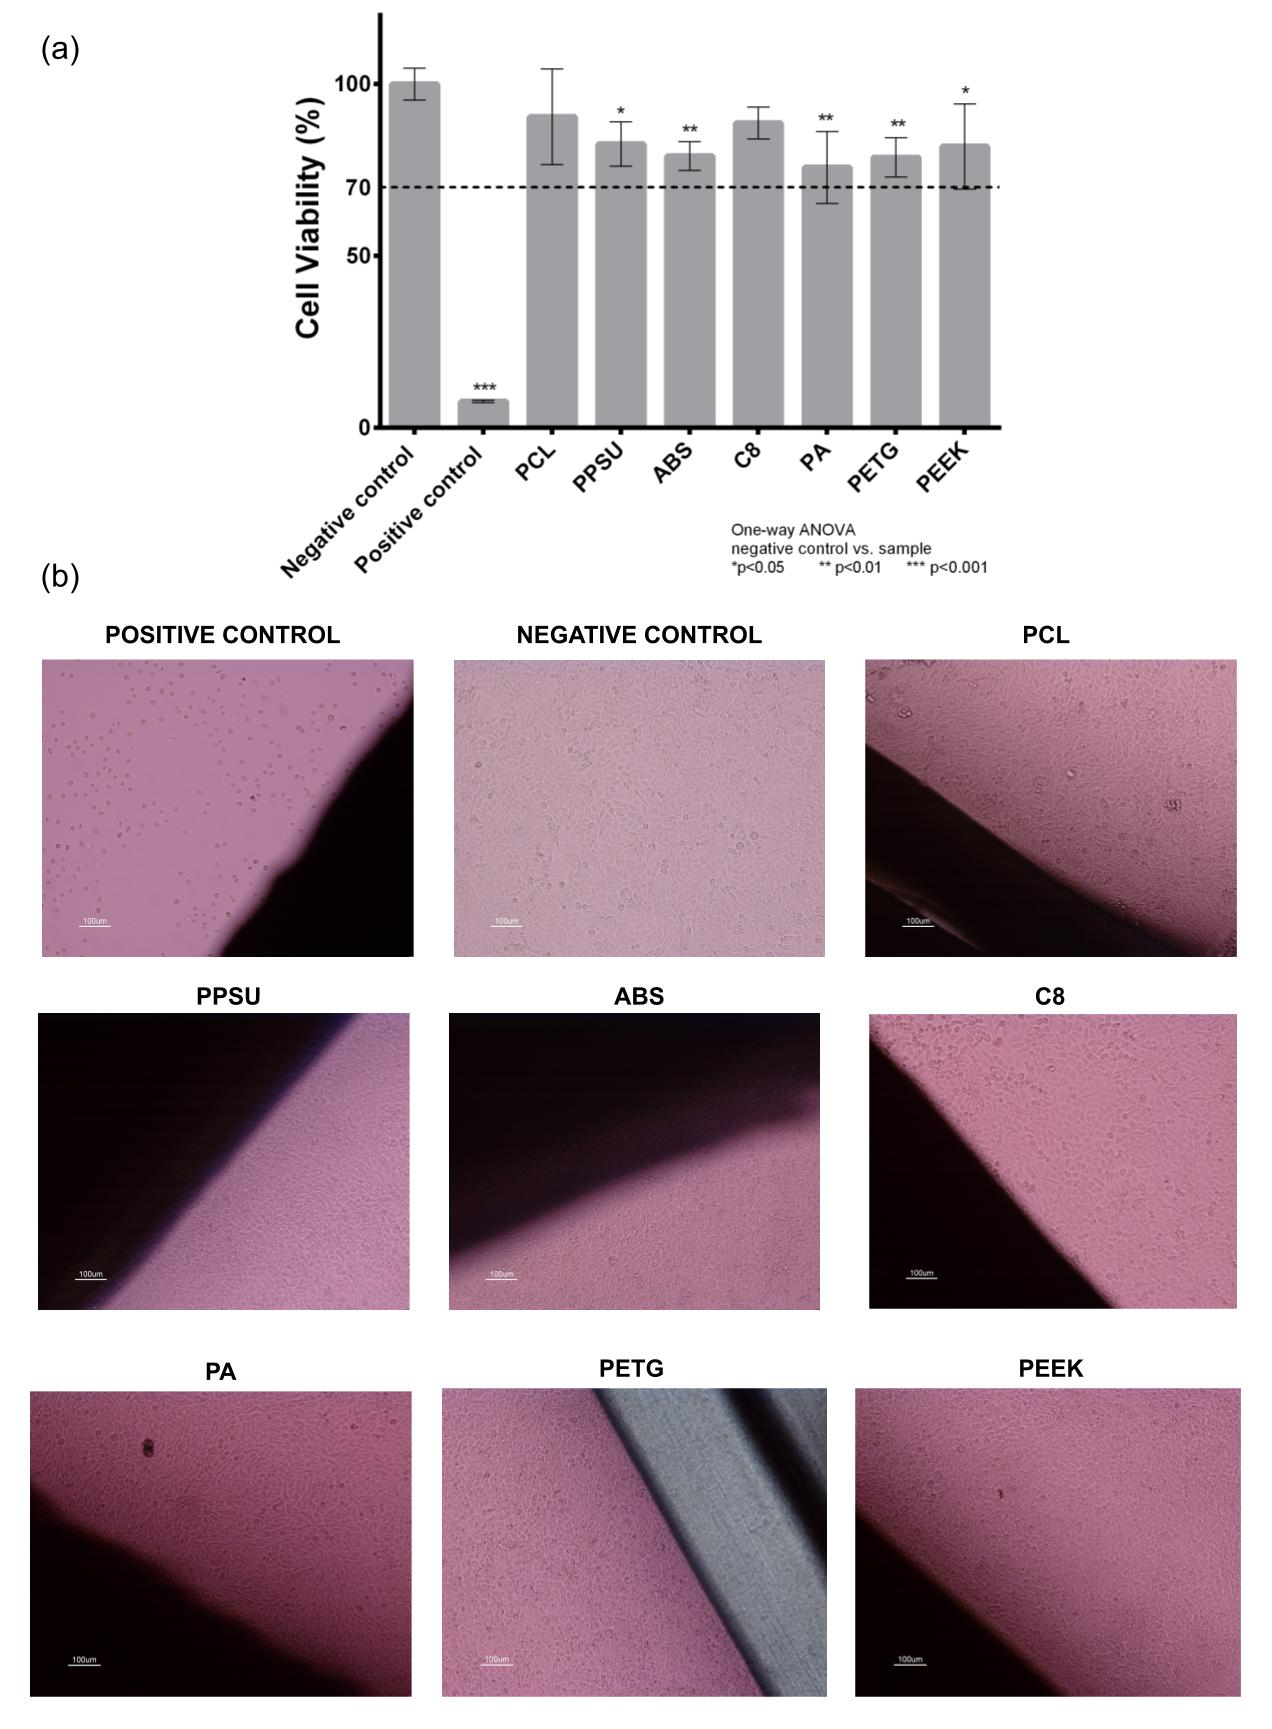
\includegraphics[scale=0.25]{./figures/Figure_6d3}}
\caption{{Cytotoxicity assay with L929 mouse fibroblast according to ISO 10993-5 standards: (\textbf{a}) indirect contact (MTT protocol); (\textbf{b}) direct contact (digital images of the material samples and the negative and positive controls, fresh culture medium and Latex, respectively). A one-way ANOVA with no corrections for multiple comparisons (Fisher’s test) statistical analysis was performed using GraphPad Prism6.}}
\label{figCito}
\end{figure}


\subsection{Bioreactor design based on model-driven decisions}
This section presents results from numerical models, starting from the predicted generated microenvironment for each bioreactor, scaffold, and holder design hypothesis considered. Then, after selecting the design that predictably generates the most osteogenic microenvironment, results from experimental validation using the developed systems are presented and compared with predictions from their numerical models. Finally, \textit{in vitro} preliminary cell culture validation results are described regarding cellular viability and metabolic activity. 


\subsubsection{Predicted bioreactor microenvironments}
The developed bioreactor design (Figure \ref{figExploded}) minimizes the culture medium volume to 45 \unit{\cubic\centi\meter}, a decrease of 91\% from our previous bioreactor version, reducing significantly culture media-related costs. This volume reduction also impacted the channel network design. From \acs{CFD} analysis, we estimated a surface average velocity magnitude of 0.120 \unit{\meter\per\second} at each scaffold holder connector channel, corresponding to an outlet velocity of 0.328 \unit{\meter\per\second} for the maximum peristaltic pump flow rate of 50 \unit{\milli\liter\per\minute} (hose connector section area of 0.0254 \unit{\square\centi\meter}). The \acs{CFD} velocity profiles of all four scaffold holder connector channels were predicted to be equal, according to the construction design strategy adopted and explained in the methods section.


\begin{figure}
\makebox[\textwidth][c]{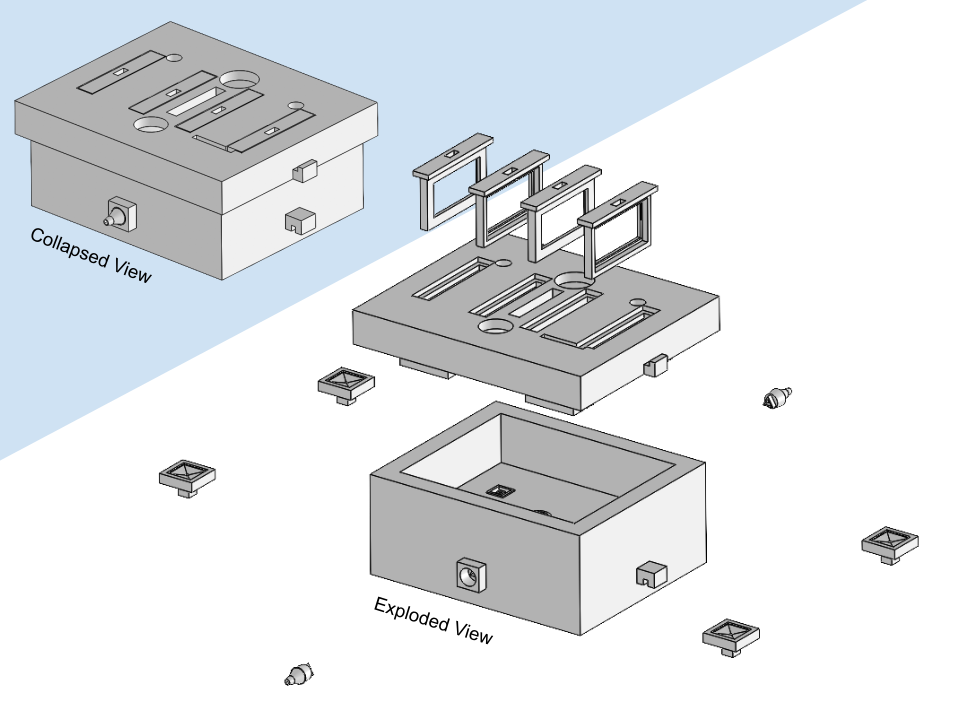
\includegraphics[scale=0.5]{./figures/Figure_6d6.png}}
\caption{Illustration of the developed bioreactor and its components. Left upper corner: assembled collapsed view. Right bottom corner: exploded view. Only the horizontal scaffold holders option is represented.}
\label{figExploded}
\end{figure}


The two holders and scaffold designs were combined into four design hypotheses (a-c, a-d, b-c, and b-d are all created combinations as shown in Figure \ref{figParts}). For the outlet's perfusion velocity (at maximum peristaltic pump flow rate), the Reynolds number predicted was within the laminar flow limits ($<0.1$ \cite{LaNasa2014-hl}) for all design combinations. Histograms for the volume distribution of the fluid-induced shear stress are presented in Figure \ref{figWSS}.

The holder at the horizontal position originates a broader shear stress spectrum for both selected scaffold geometries. Once we are using the maximum peristaltic pump flow rate, this means that the horizontal holder configuration is the only one that may allow us to tune the fluid-induced shear stress by decreasing/increasing the peristaltic pump flow rate debit if required. In in the original manuscript supplementary materials Figure S8a, the impact of changing the peristaltic pump flow rate is exemplified, an action that will allow fitting the fluid flow-induced shear stress to a recommended cellular range of mechanical stimulation. Even considering the outcomes of the considered maximum peristaltic pump flow rate, at cell culture ROI, if both scaffold designs were placed in the horizontal holder, both would be able to generate a microenvironment inside the reported osteogenic ranges, 0.0015-0.024 \unit{\pascal} \cite{Vetsch2017-zd}, 0.00020-0.013 \unit{\pascal} \cite{Yamada2021-qf}, (Figure \ref{figWSS}, original manuscript supplementary Figure S8b). It is observable in the numerical predictions (Figure \ref{figWSS}), for all considered scaffold and holder combined geometries, that most of the volume fractions values occur within a range from 0 to 0.1 \unit{\pascal}. Remarkably, the horizontal holder and orthogonal scaffold combination show most of the predicted volume fractions in a range of 0 to 0.02 \unit{\pascal}, already inside the reported osteogenic ranges.


\begin{sidewaysfigure}
\centering
\includegraphics[width=\textwidth]{./figures/Figure_6d7.png}
\caption{Relative volumetric distribution of the fluid-induced shear stress (in units of \unit{\pascal}) for all combinations of selected scaffolds and holders, predicted by the \acs{CFD} numerical model at the culture \acs{ROI}. The maximum peristaltic pump rate of 50 \unit{\milli\liter\per\minute} was considered at the outlet. The volume axis refers to the number of node occurrences of the correspondent shear stress in the \acs{ROI}, normalized to its peak value.}
\label{figWSS}
\end{sidewaysfigure}


The horizontal holder was then selected since it provided optimal fluid-induced shear stress conditions for osteogenic effects, and the predicted volumetric distributions of the electric field for this holder and the established protocol were compared (see methods section). 

When comparing both scaffold geometries placed upon the horizontal holder (Figure \ref{figEF}), the orthogonal scaffold is the one with a higher \acs{EF} magnitude predicted at culture \acs{ROI}, with an average value of 0.118 \unit{\volt\per\meter}. In comparison, the honeycomb scaffold has an average electric field magnitude of 0.035 \unit{\volt\per\meter}. The observed non-uniformity of the electric field follows previously reported studies \cite{Meneses2021-nd}. These prediction results are caused by the presence of a scaffold structure that introduces an obstacle to the flow of charges (original manuscript supplementary Figure S8b). The effect of the scaffold's presence on the electric field in the surrounding culture medium is mainly determined by its geometry and by the difference in electrical conductivity of the scaffold materials and surrounding culture medium. Combining the horizontal holder with the orthogonal scaffold thus allows for a broader range of multimodal stimulation (simultaneous fluid-induced shear stress and \acs{EF}). For this reason, this was the hypothesis selected for fabrication and subsequent validation.



\begin{sidewaysfigure}
\centering
\includegraphics[width=\textwidth]{./figures/Figure_6d8.png}
\caption{Relative volumetric distribution of the electric field magnitude (\unit{\volt\per\meter}) for all combinations of scaffolds and holders when subjected to the \acs{CCoupled} stimulation (sine wave, 60 \unit{\kilo\hertz}, 10 \unit{\volt}p-p). All data was obtained from frequency domain \acs{EF} numerical model predictions at the culture \acs{ROI}. The volume axis refers to the number of node occurrences of the correspondent \acs{EF} magnitude in the \acs{ROI}, normalized to its peak value.}
\label{figEF}
\end{sidewaysfigure}


\subsection{Fabrication and pre-culture validation}
Bioreactor parts, selected scaffold, and holder structures were \acs{3D} printed as described in the methods section. Systems electronics were assembled, and probes were inserted into their established positions inside the bioreactor. Pre-culture tests were performed as described in the methods section (further details in original manuscript supplementary materials). The bioreactor produced in \acs{C8} composite material and externally coated in PDMS presented no water leaks in the watertight test after 24 \si{\hour} at 37 \unit{\celsius}, external or internal (infill space). The 24 \si{\hour} continuous perfusion test was successful, \textit{i.e.} the developed perfusion system sustained the required liquid level for that period. The individual operation of each applied sensor was confirmed in terms of stability and performance. Micro-computed tomography applied to the produced \ac{PCL} orthogonal scaffold samples revealed a mean pore size of $490 \pm 30$ \unit{\micro\meter} and a mean filament diameter of $518 \pm 30$ \unit{\micro\meter}, which are within the values originally established for both properties. 

Perfusion velocity measurements corresponded well to the numerical model predictions for the fluid flow at the bioreactor culture chamber without scaffold structures, as seen in Figure \ref{figValidation}(a). The two-time points, 13 \si{\second} 042 \si{\milli\second}, 16 \si{\second} 005 \si{\milli\second}, correspond to a yellow dye movement of 7 \si{\milli\meter} on top of the scaffold holder, which results in a mean velocity of 2.36 \si{\milli\meter\per\second}, following the numerical prediction (2-3 \si{\milli\meter\per\second}) for the same region and conditions. 

Regarding the \acs{CCoupled} stimulation system, the numerical model predicts an \acs{EF} of \num{0.095} \si{\volt\per\meter} and an electric current of \num{3.21d-5} \si{\ampere} at the testing setup (using the material properties and values from Table \ref{table61}). The experimental value of the electric current on the testing setup was \num{2.43d-5} \si{\ampere} (measured across a resistor with \num{21.89} \si{\kilo\ohm}, Figure \ref{figValidation}(b)). Using the developed \acs{FEM} model and setting a floating potential boundary condition for these two currents, the model predicts an electric field magnitude of 0.072 \si{\volt\per\meter} (for 24 \si{\micro\ampere}) and 0.095 \si{\volt\per\meter} (for 32 \si{\micro\ampere}). A numerical prediction with a 24\% difference for the same region and conditions, that at this scale could have been caused by model imprecisions in material properties. The developed \acs{CCoupled} stimulation system model neglected the \num{21.89} \si{\kilo\ohm} resistor used to perform the measurement currents. If accounted for (by means of a circuit terminal boundary condition), it would drop the predicted electric field magnitude to 0.094 \si{\volt\per\meter} (with a predicted current of \num{31.8} \si{\micro\ampere}). Despite being neglected in the developed system model, due to its narrow impact, adaptations of this \acs{CCoupled} stimulation system that change any of its main components should reconsider the measurement resistor impact.    


\begin{figure}
\centering
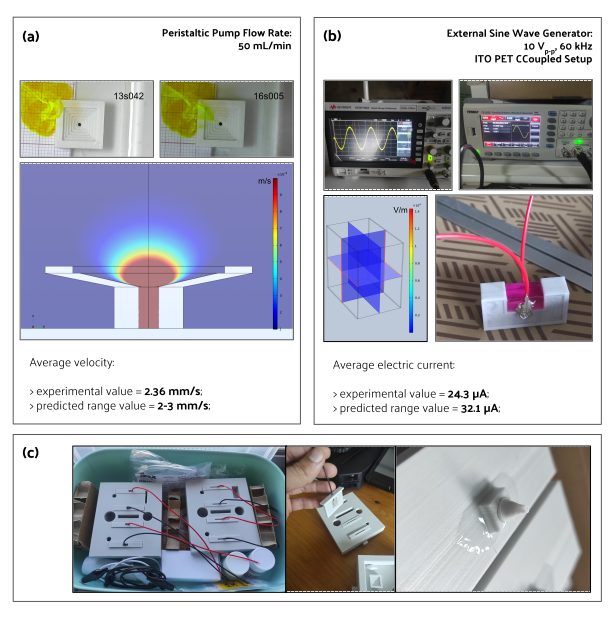
\includegraphics[width=\textwidth]{./figures/Figure_6d9.png}
\caption{Pre-culture validation of the fabricated perfusion bioreactor and its \acs{CCoupled} system and comparison with the numerical model's predictions for (a) fluid flow velocity and (b) electric current generated. The \acs{EF} generated by the \acs{CCoupled} system validation setup was predicted to be uniform, with a value of 0.095 \unit{\volt\per\meter} at the culture medium region. (c) Photos from the assembled bioreactor, electrodes, and perfusion connectors.}
\label{figValidation}
\end{figure}


\subsection{\textit{In vitro} cell culture viability and metabolic activity validation}
The preliminary validation results of the fabricated perfusion bioreactor and its \acs{CCoupled} system showed an applied \acs{EF} magnitude volume average of 0.118 \unit{\volt\per\meter}, which does not appear to impact the viability of human MG-63 osteoblasts. High cell viability was observed with no evidence of cell death in all conditions, as shown in Figure \ref{figViability}. Nonetheless, a significant effect is observed for this cell line when comparing cell-seeded scaffolds cultured in 24-well plates versus the bioreactor (no perfusion condition), with the latter presenting inferior metabolic activity (Figure \ref{figMetabolic}) but maintaining high cell viability and spreading around the scaffold (Figure \ref{figViability}). Overall, the validation tests confirmed that the fabricated bioreactor design can support cell cultures without signs of cytotoxicity or reduced cellular viability.


\begin{sidewaysfigure}
\makebox[\textwidth][c]{\includegraphics[scale=1.0]{./figures/Figure_6d10.png}}
\caption{Results from the bioreactor preliminary human MG-63 osteoblasts cell culture viability tests performed with LIVE/DEAD staining at day 14 (after 3x \acs{CCoupled} stimulation and 48h bioreactor culture).}
\label{figViability}
\end{sidewaysfigure}

\begin{figure}
\centering
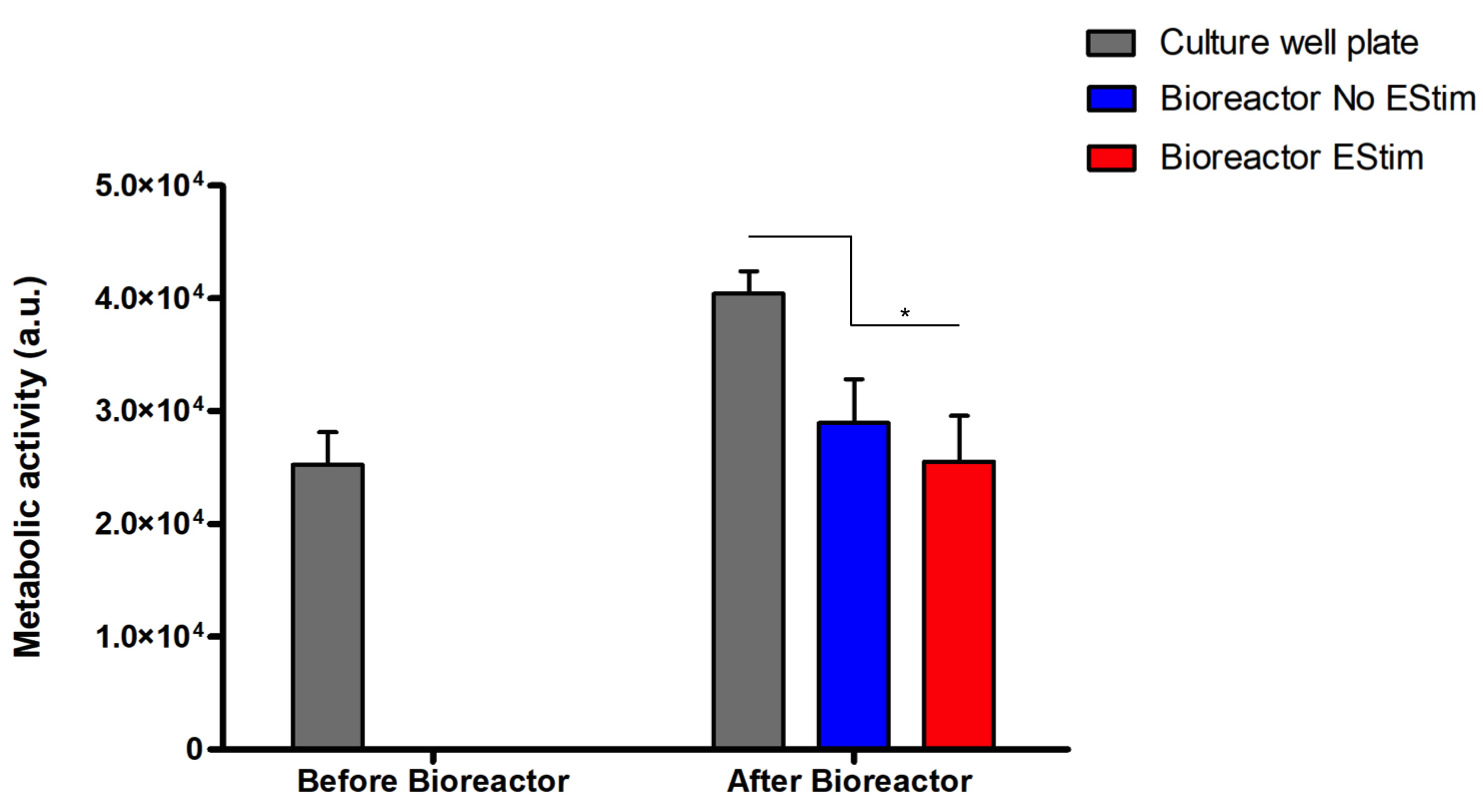
\includegraphics[width=\textwidth]{./figures/Figure_6d11.png}
\caption{Results from the metabolic activity of human MG-63 osteoblasts on a bioreactor preliminary static cell culture. Results present time points before (Day 12) and after bioreactor culture (Day 14) with/without \acs{CCoupled} stimulation. * account for significant differences $p<0.05$.}
\label{figMetabolic}
\end{figure}




\section{Discussion and limitations}
From a bird's eye view, the developed bioreactor design is one of many possibilities that can be obtained if considering different starting points, actuation strategies, and goals to be achieved. Nonetheless, the development strategy ensures that the produced design complies with the application of predetermined stimulation environmental conditions, even when applied simultaneously, like combined fluid-induced shear stress and \acs{EF} stimulation. 

\subsection{\textit{In vitro} cytotoxicity tests}
Accordingly, in the direct contact test, cells cultured in contact with all the materials presented normal fibroblast morphology with no evidence of any inhibition halo effect or cell death. According to the cytotoxicity test results, all candidate materials are suitable for our bioreactor additive fabrication. We picked \acs{C8} as the material of main interest for future design fabrication. \acs{C8} is a new material with good layer adhesion and surface quality, which are key features for perfusion flow. The \acs{C8} supplier datasheet reveals that this material has a higher tensile strength than ABS, resulting in improved mechanical characteristics, which are important for the overall robustness of the bioreactor to withstand the tightness of pressure chambers.


\subsection{Decisions on bioreactor fabrication}
We used numerical models to update the geometry or the stimulation protocol until established microenvironment properties were achieved. This iterative strategy is only possible if the resultant bioreactor design can be fabricated with high precision, a premise obtained through additive manufacturing technologies \cite{Gensler2020-in}. Various concepts of perfusion bioreactors \cite{Smith2018-he, Daneshgar2019-tu, Gabetti2022-hp, Birru2018-rj} have been \acs{3D} printed with stereolithography technology using class I biomaterial dental resin, while others have used fuse deposition modelling technology \cite{Rosser2018-zg, Schmid2018-rg, Raveling2018-gl}. A challenge with fuse deposition modelling 3D prints is to obtain leakproof components, since this process usually generates highly porous structures between filaments deposition. Different solutions were applied to overcome this issue. One approach was to cast an acrylonitrile butadiene styrene (ABS) part with a type of silicone rubber that cures at room temperature (commercially known as RTV silicone), creating a part mold and filling it with a two-part polyurethane casting resin \cite{Rosser2018-zg, Schmid2018-rg}. Another approach was to 3D print the bioreactor in ABS and waterproof it by treating its parts with an acetone vapor bath \cite{Raveling2018-gl}. In the present study, the bioreactor device was 3D printed, and afterward, all its 3D-printed pieces were coated with an external PDMS coating to achieve a watertight structure. Theoretically, it is possible to produce fuse deposition modelling leakproof parts without any added coating using larger nozzles and higher filament superposition. However, in a natural setting, this remains challenging due to small manufacturer imprecisions that occur during the printing process. Using an external coating allowed us to correct imprecisions that may have occurred during the 3D printing process.


\subsection{Bioreactor inner environment}
Some bioreactor-based strategies targetting bone regeneration are scaffoldless, like the one from Smith \textit{et al.} \cite{Smith2018-he} that uses a Kenzan micro-needle array; others support a single scaffold or single tissue sample \cite{Daneshgar2019-tu, Gabetti2022-hp, Schmid2018-rg, Rosser2018-zg, Birru2018-rj, Visone2018-sa}. Our design can support four scaffold structures under identical conditions in the same bioreactor. The operation concept behind our design is also flexible to expand to support even more scaffold structures.

The capability to monitor the fluid flow or electric phenomena in the presence of the scaffold structure and cellular content may be crucial to update and take more advantage of numerical models, extending their application into the monitoring and controlling of the cell culture microenvironment during the entire culture phase. Smith \textit{et al.} \cite{Smith2018-he} integrated a Doppler ultrasound imaging system to assess the flow characteristics inside the bioreactor culture chamber. Abasi \textit{et al.} \cite{Abasi2020-fn} proposed an electrical stimulation system that includes real-time monitoring of the response of a cellular membrane via AC electrical impedance spectroscopy. This design hypothesis may be fruitful in understanding electric changes in the cultured tissue. Our developed bioreactor uses commercially available sensors to perform real-time monitoring of pH, dissolved oxygen, and temperature fluctuations. However, there is still room for improvement regarding more accurate and less invasive procedures and/or miniaturized sensors.

Regarding multimodal stimulation approaches (fluid flow-induced shear stress and electromagnetic), the bioreactor designs from Gabetti \textit{et al.} \cite{Gabetti2022-hp} and Visone \textit{et al.} \cite{Visone2018-sa} are only two of the few examples of uni/bi-directional perfusion and simultaneous stimulation with a pulsed electromagnetic field. Visone \textit{et al.} \cite{Visone2018-sa} also introduced an original design that allows a microscopic observation of the cell culture without exposing it to an external environment. Our proposed bioreactor approach similarly allows the delivery of uni/bi-directional perfusion, alone or combined with an electric field stimulation system, conceived as capacitively coupled to induce a pure electric field to the cell cultures inside the bioreactor and avoid cell toxicity due to faradaic products that can occur in direct-coupled systems. Our current design capabilities can be further expanded with actuators to control temperature and O\textsubscript{2} / CO\textsubscript{2} gas concentrations, incorporating a system similar to the one described by Samokhin \textit{et al.} \cite{Samokhin2022-oy}.


\subsection{Bioreactor validation}
Once fabricated and before the introduction of \textit{in vitro} cell culture tests, the bioreactor was subjected to a pre-validation experiment to confirm if the conditions predicted in the numerical models are verified in the physical bioreactor system. Pre-culture validation results were in close correspondence with the experimental measures. Fluid flow velocity measurement was based on a video recording of a yellow dye wavefront movement, and the velocity was estimated using correspondent elapsed time between two known positions. This measurement was performed without a scaffold to improve the camera's field of view over the dye flow. The recorded fluid flow velocity (2.36 \si{\milli\meter\per\second}) matched the numerical predicted range for the same scaffoldless conditions at that same region (2-3 mm/s). Despite this agreement, more accurate techniques, like micro-particle image velocimetry \cite{Guastamacchia2022-bf} or ultrasound \cite{Smith2018-he}, could be applied to reconstruct velocity and shear stress fields in the presence of scaffold structures, allowing for comparison of CFD numerical models and experimental results with greater detail. \acs{EF} are difficult to measure directly, so we choose to determine their value by measuring the total electric current across a resistor in series with the CCoupled testing setup. A specially designed validation setup was built for the CCoupled system to spend less volume of culture medium, while keeping identical conditions to the cell culture chamber without any scaffold or holder structures. The developed numerical model of this testing setup predicted a current of \num{3.21d-5} \unit{\ampere}, higher than the measured value (\num{2.43d-5} \unit{\ampere}), but of the same order of magnitude. This slight overestimation may be caused by the material electrical properties adopted based on previous literature-reported values. This model should be further refined with electronic impedance spectrum characterization of the involved materials, since impedance may relate to the applied signal frequency \cite{10261_305757}. Natural bone streaming potentials are thought to be in the proximity of \num{0.39} $\pm$ \num{0.14} \si{\milli\volt} \cite{Qin2002-bn}, electric potentials that can be currently generated in the ROI using the developed CCoupled system by lowering the amplitude of the applied sinusoidal wave.

Pre-culture validation was essential to confirm that numerical model predictions and experimental measures obtained were in close agreement. This approach serves two primary purposes: first, differences can help improve both models and design/fabrication procedures; second, matching values increases the confidence in our pipeline for bioreactor design and fabrication. Thus, we recommend that future studies using numerical models to fine-tune the 3D design of bioreactors should include pre-validation assessments.


\subsection{Numerical modelling approaches}
Multiple studies on bioreactor concepts introduced numerical models to predict the applied microenvironment conditions. Usually, these studies applied \acs{CFD} models to empty chamber bioreactor digital designs to calculate flow regimes, velocity profile, and flow-induced shear stress \cite{Smith2018-he, Daneshgar2019-tu, Gabetti2022-hp, Rosser2018-zg, Schmid2018-rg, Visone2018-sa, Lim2019-gx}. Gabetti \textit{et al.} \cite{Gabetti2022-hp} also performed electromagnetic field simulations to predict the distribution of the delivered magnetic field, and Visone \textit{et al.} \cite{Visone2018-sa} performed an electric field estimation very similar to the one performed in our work. Compared with our modelling strategy, these previous studies did not modify the bioreactor design interactively to adjust microenvironment predictions, thus limiting microenvironment adjustments using only external manipulation. Also, these works did not include models with scaffold structures, which are widely used in \acs{TE} strategies and can powerfully shape fluid flow and electric field delivery. One improvement that may need to be addressed by future models is the need to introduce scaffold surface topology, since different scaffold surface properties will introduce local fluid flow-induced shear stresses that may be relevant in the generated biological response. Numerical models have commonly been used in isolation as alternatives to experimental measurements. However, with our approach, we demonstrate that it is a good practice to establish a VVUQ (verification–validation–uncertainty quantification) procedure when dealing with numerical models to cross-validate the model and bioreactor/scaffold fabrication before the cell culture studies phase.


\subsection{\textit{In vitro} cell culture tests}
Preliminary cell culture validation was performed with human osteoblast-like MG-63 cells, a cell type usually applied in osteogenic-related studies \cite{Ghanbari2023-du, Dehkordi2022-ku}. Although cell viability remained impaired, cell metabolic activity was affected when the scaffolds with seeded cells were transferred from the well plate to the bioreactor. The decrease in metabolic activity was further enhanced by the application of a low-intensity\acs{EF} (0.118 \unit{\volt\per\meter}), an effect also observed by Cohly \textit{et al.} \cite{Cohly2003-hm} after applying a static electromagnetic field on the human MG-63 osteoblast cell line. MG-63 cells exposed to the static electromagnetic field \cite{Cohly2003-hm} were reported to have a 34\% decrease in proliferation, 37\% decrease in the secretion of proline, a significant component of collagen, and down-regulation of collagen I, alkaline phosphatase, parathyroid hormone-receptor, and osteocalcin mRNAs. Cohly \textit{et al.} \cite{Cohly2003-hm} concluded that exposure to very low static electric fields affects the human MG-63 osteoblasts in a manner that may be detrimental to bone formation. Our preliminary cell culture validation was performed under non-perfused conditions since our focus was first to test the cellular viability response when subjected to the \acs{EF} from the developed \acs{CCoupled} system compared to the well plate control conditions. \acs{CCoupled} systems are used less often in \acs{TE} applications than ubiquitous perfusion systems, justifying more attention in an initial application. Future work will include cell culture validations under different fluid flow profiles in combination with different \acs{EF} magnitudes to ascertain the definite effects on cell viability, proliferation, and osteogenic differentiation.    


\subsection{Reproducibility: open-source solutions}
Despite the diversity of bioreactor solutions currently available, to the best of our knowledge, only a handful of designs have been shared open-source with complete fabrication blueprints \cite{Daneshgar2019-tu, Raveling2018-gl}. Most of the bioreactor designs found only briefly describe the fabrication methodology, usually with insufficient detail to allow its precise replication. This hampers reproducibility for other studies due to hard-to-guess geometrical dimensions and material properties, profoundly impacting microenvironmental conditions during external stimulation. As the extensive review from Nicksic \textit{et al.} \cite{Nicksic2022-jy} points out, retrieving conclusions from electric stimulation studies are challenging due to a substantial variability in protocol definition, stimulation conditions, and device specification reports, which are usually incomplete. We aim to overcome these issues by releasing all outputs from our JANUS approach under a public open-source Attribution-ShareAlike 4.0 International license (https://doi.org/10.5281/zenodo.7695700). We have included blueprints for the fabrication of this bioreactor/scaffold, electronic schematics, a detailed list of used components with their correspondent part reference, and all developed source files for numerical models (also shared with a complete report of its parametrization), control firmware and software. An overall cost estimate for fabricating a replica of this developed bioreactor is also presented in the original manuscript supplementary materials, along with a detailed development roadmap.


\subsection{The central relevance of JANUS}
JANUS combines a particular 3D printable bioreactor/ scaffold design and its numerical models. This work focused on using this model prediction data-driven design strategy to recreate targeted cellular microenvironments. Introducing the scaffold structure into the bioreactor numerical model is critical to further understand the conditions that have been created. Their geometry and material properties will become part of the cell microenvironment, affecting the way the fluid flows, thus shaping the mechanical stimulation \cite{Capuana2023-ik, Moradkhani2021-qf, Zhao2018-ci, Zhao2020-pa} and affecting the way that electric/ionic currents might interfere with electrical stimulation delivery \cite{Meneses2021-nd}. The generated microenvironment is expected to be as predicted by numerical models before cell seeding occurs. However, once cells are added to the scaffold, the microenvironment will change considerably due to cell proliferation and extracellular matrix secretion that fills the volumes once occupied by the culture medium, modifying scaffold topology and closing its pores. Previous studies have reported these effects and offer a window into the impact of cellular activity and growth on stimulation delivery \cite{Zhao2020-pa, Perier-Metz2021-bj}. These studies introduce cellular models into a chain of other existent models of bioreactor/scaffold microenvironment conditions, like the one we presented here, so stimulation delivery could be better predicted and modified, accounting for posterior cellular activity changes. Future work may elaborate on adding cellular models to this work baseline models and improve bioreactor design with control and actuation features, evenly introducing machine learning capabilities for real-time culture monitorization. Future work will also include long-term cell cultures to verify the performance of the developed bioreactor design for longer periods (from weeks to months). 

The JANUS duality (virtual-physical) can still be helpful after the experimental setup design and stimulation protocol are set by helping to control and adjust the microenvironment to maintain the adequate \textit{in vitro} conditions: for example, keeping an appropriate level of fluid-induced shear stress that induces differentiation of progenitor cells towards an osteoblastic lineage on 3D scaffolds in the absence of chemical stimulation \cite{Yamada2021-qf}. Another advantage of the virtual-physical combination is to improve the comparison between protocols from different studies by allowing them to match other reported experimental conditions or serve as the baseline to feed further numerical models that account for cell seeding and neotissue metabolism, growth and proliferation \cite{Reina-Romo2019-ry}.


\section{Summary}
In a nutshell, we presented a strategy to design multimodal bioreactors based on numerical model-driven decisions regarding the predicted microenvironment generated by the set of a particular bioreactor/scaffold geometries when applied with a specific stimulation protocol. Furthermore, we showed that combining physical and virtual approaches may improve the precision when constructing stimulation setups and applying cell culture stimulations, allowing for better control and overall replicability of experimental outcomes. The resulting perfusion bioreactor design was experimentally validated, capable of simultaneous mechanic and \acs{EF} stimulation. It is made available open source in an online platform with all its blueprints and fabrication instructions. This bioreactor virtual-physical strategy could also be helpful to drop experimental costs, allowing to optimize culture medium usage and the number of required bioreactors.

This chapter demonstrates that numerical models can help to design, predict, and confirm environmental properties generated at or by bioreactors, allowing the translation of previously reported works into new designs. These numerical models can also be applied to refine protocols to increase the desired biological responses or to confirm new protocol hypotheses. It is expected that bioreactor approaches like JANUS can lead to more favorable environmental conditions to improve cellular outcomes like differentiation, migration, and proliferation.




%\newpage
%\bibliography{library_c6} 
%\bibliographystyle{plain}
%\end{document}
%\documentclass[11pt]{report}
%\usepackage{siunitx}
%\usepackage{graphicx}
%\usepackage[table,xcdraw]{xcolor}
%\usepackage{csquotes}

%\begin{document}
%\setcounter{chapter}{6}
%\tableofcontents


\newpage
\chapter{Global Discussion}
This chapter presents an overall discussion of this dissertation content, starting from summarising its key findings, understanding the major limitations present in the current work, and pointing to future perspectives of the work developed.



\newpage
\section{Main outcomes of this work}

As seen in the previous chapters, the application of numerical modelling techniques to perform predictions in \acs{BTE} stimulation contexts can be an essential tool to optimize and control the induced effects in \textit{in vitro} cell cultures. Numerical models, using finite-element methods and lumped-element methods (electric circuit analogs) were used to predict \textit{in vitro} microenvironmental conditions produced by developed and reported experimental setups under known inputs. This kind of numerical modelling framework was able to provide precise estimates of the delivered E-Field (Chapters 4, 5, and 6) or fluid flow-induced shear stress (Chapters 3 and 6) in the cell culture region for a specific combination of bioreactor setup and scaffold geometry. Best practices \cite{Klein2022-yj} point out the importance of validating the numerical model predictions with experimental measurable outcomes and confronting them with the corresponding model prediction. This study was performed in Chapter 6 for systems delivering \acs{EF} and fluid flow-induced shear stress. This work was committed to effectively share all developed systems and models under an open-source licensing attribution for scientific purposes, including configuration files for hardware, firmware, software, fabrication blueprints, analyzed data, \acs{CAD} files, and many others required to reconstruct the developed physical setups, stimulation systems, and their corresponding digital models. In this way, this work contributes to fill in the existent gap in the scientific reproducibility and strengthens the need for developing common practices for stimulation protocols and bioreactor \textit{in vitro} cell culture operation for \acs{BTE} and other \acs{TE} areas. It is possible to compare the current version of the developed bioreactor with a list of key features required for a proposed ideal bioreactor system as identified by Ahmed \textit{et al.} \cite{Ahmed2019-uk}. This comparison is available in Table \ref{tabBioreactor}, where we can observe that the current bioreactor development integrates most of the critical features previously identified as essential, and also expands these to include easy and precise reproducibility by designing it specifically to be produced using \acs{3D} printing fuse deposition modelling fabrication. 


\begin{table}[ht]
\caption{Comparison between “must have” features that a new generation of bioreactors should include according to Ahmed \textit{et al.} \cite{Ahmed2019-uk} and current JANUS bioreactor features.}
\bigskip
\scriptsize
\centering
\begin{tabularx}{370px}{l l c} \toprule[0.15em]
\textbf{Features} & \textbf{Advantages} & \textbf{JANUS Bioreactor} \\ \cmidrule(l){1-3}
\rowcolor[HTML]{EEEEEE} 
\textit{Leakproof} & Reduces the risk of contamination and loss of reagents. & {\color[HTML]{38761D} \textbf{TRUE}}  \\
\rowcolor[HTML]{FFFFFF} 
\textit{Optically Transparent} & Allows in situ real-time monitoring. & {\color[HTML]{FF0000} \textbf{FALSE}} \\
\rowcolor[HTML]{EEEEEE} 
\textit{Easy to Assemble} & Less training required, rapid experimental set-up. & {\color[HTML]{38761D} \textbf{TRUE}}  \\
\rowcolor[HTML]{FFFFFF} 
\textit{Ability to monitor} & Provide data on culture conditions such as pH, & \\ 
\textit{microenvironment} & oxygen, carbon dioxide, metabolites. & {\color[HTML]{38761D} \textbf{TRUE}} \\
\rowcolor[HTML]{EEEEEE} 
\textit{Allows use of different flow} & Different flow rates/types are required & \\
\rowcolor[HTML]{EEEEEE} 
\textit{types/rates} & for different cell types/applications. & {\color[HTML]{38761D} \textbf{TRUE}} \\
\rowcolor[HTML]{FFFFFF} 
\textit{Allows easy insertion and} & Allow 3D cell culture and post-analysis. & \\
\textit{retrieval of scaffolds} & & {\color[HTML]{38761D} \textbf{TRUE}} \\ 
\rowcolor[HTML]{EEEEEE} 
\textit{High throughput} & Faster data acquisition. & {\color[HTML]{38761D} \textbf{TRUE}} \\ 
\rowcolor[HTML]{FFFFFF} 
\textit{Flexible configuration} & Modular interconnected systems allow co-culture and & \\
& cell-cell signaling & {\color[HTML]{38761D} \textbf{TRUE}}  \\
\rowcolor[HTML]{EEEEEE} 
\textit{No air bubble formation} & The presence of air bubbles can disrupt the flow rate and  & \\
\rowcolor[HTML]{EEEEEE} 
 & disturb cells. & {\color[HTML]{38761D} \textbf{TRUE}}  \\ \bottomrule[0.15em] 
\end{tabularx}
\label{tabBioreactor}
\end{table}


As shown in Chapter 5, numerical models can also be used to perform meta-analyses of literature-reported setups and protocols. Eight \acs{CCoupled} setups, that were used in twenty studies published between 1978 and 2021, were reproduced and analyzed numerically to observe if the reported \acs{EF} matched the numerical prediction of three different models. It was found that the \acs{EF} was correctly estimated in only 3 out of 8 setups. In 12 out of 20 studies, the overestimation may have led to incorrect assumptions on the effects of stimulation on the observed cellular effects, thus requiring reinterpretation. Numerical models can also be useful to adapt stimulation protocols for different stimulation setups, integrating previously reported results from the literature in recent designs, and additionally, allowing for more reliable comparisons between different experimental outcomes. Methods and results from Chapter 4 for \acs{DCoupled} stimulation setups, regarding experimental protocols and their biologically produced effects can be further refined, by exploring further the experimental characterization of the phenomena involved (electrochemical impedance spectroscopy of the materials involved, electric double layer response, ionic mobility, etc), gathering data that can be introduced into numerical models, contributing to a deeper knowledge of the stimulation phenomena and related biological effects. 

Finally, this work introduced a scaffold structure into the empty cell culture chamber numerical models. The presence of a scaffold in a cell culture, considering its specific geometry and material properties, was shown in Chapters 5 and 6 to have a crucial influence in the generated \acs{EF} and fluid flow-induced shear stress stimulation delivered to the cell culture. The impact of this structure and eventual morphology deviations among the produced scaffolds (when compared to the geometrical ground truth) should be considered in simulation predictions and accounted for as a variability source, often neglected in experimental studies. 




\section{General limitations of this work}

\acs{FEM} was the numerical modelling technique most applied in this research. Recursively applied to different systems/setups geometries and material characteristics, it was essentially reduced to two major sets of equations implemented by COMSOL Multiphysics: one considering the physical phenomena of fluid laminar flow and the other considering electric currents. The considered setup geometries (bioreactors, culture wells, scaffolds) are geometrically simple, however when combined under the same model, require a larger complexity of the mesh to be computed, which had to be adapted for different size scales differing by an order of \num{d6} or higher. This added unprecedented complexity to the model, increasing the computational time required to find a solution, which may originate non-linear and singularity errors, specifically for coarse meshes, limiting the execution of mesh-independent studies. This difficulty was circumvented by considering the finner mesh possible to run on the physical machine available and by selecting a solver with adaptative mesh refinement \cite{Verfuhrt1996-hy}.

Material properties that feed the constructed numerical models were mostly obtained from the literature, an option that induces uncertainty upon the validation of the developed model with a particular setup and cell culture conditions. To decrease this uncertainty, an extensive material characterization should be performed, for example, to determine the response of a particular material to an electric current / electric potential application through experimental techniques, such as impedance spectroscopy, cyclic voltammetry, and chronoamperometry. If this material composes an electrode, its interface with the electrolyte should also be extensively characterized.    

Although this work used well-established electric currents and laminar fluid flow models, other physical/chemical phenomena, not covered by the applied modelling frameworks, may also contribute to the observable biological effects. For example, electrophoresis or dielectrophoresis responses may occur when using electric stimulation signals. These are defined as the motion of suspended particles (including mammalian cells) caused by polarization effects in inhomogeneous electric fields. All particles exhibit dielectrophoretic activity in the presence of electric fields \cite{Park2020-lj, Pethig_undated-bv}. However, the strength of the force depends strongly on the medium and particles' electrical properties, on the particles' shape and size, as well as on the frequency of the electric field. Consequently, fields of a particular frequency can manipulate particles with great selectivity. Another limiting assumption is that
the culture medium is typically assumed to be a homogeneous distribution of chemical species, however, external stimulation might originate heterogeneous space regions with a specific concentration of chemical species, that may constitute probable cause for some effects that cannot be directly attributed to the applied \acs{EF} magnitude. Ratchetaxis phenomena, for example, suggest that cell motility can be viewed as a stochastic phenomenon, which can be biased by various types of local cues, leading to directional migration, which includes electric and shear stress interactions \cite{Zhao2011-wy}, and also cues from cell attachment surface topology, chemical gradients, mechanical stiffness, among others \cite{Caballero2015-cs, Pieuchot2018-kl}. 




\section{Future work}
The evolution of this work can be expected to occur in each of the three main axes addressed in this work: experimental setup design and fabrication; correspondent numerical model construction and validation; and new cell culture stimulation protocols. 

Bioreactor design represents a continuous and laborious effort. Our JANUS design represents the end of a work journey, but not the end of the development line. Future versions should include an improved set of optical sensors (to avoid electromagnetic interference from the electrical stimulation) and become completely watertight and autoclave sterilizable immediately after the \acs{3D} printed process, without requiring further coating applications. Once specifically optimized for that purpose \acs{3D} printing processes have shown to be capable of producing parts without deformation, made from polymeric materials that endure typical autoclave sterilization processes, like polycarbonate, polystyrene, polyetherketoneketone or polyetherimide. Watertight and sterilizable outcomes could then be achieved with high-performance fuse deposition modelling printers by using large nozzles, closed warm chambers, and high processing temperatures. 

These updates will enable an even more reusable bioreactor capable of sustaining a series of experimental works to characterize a precursor cell response to isolated or combined electrical and mechanical stimuli, an experiment where all protocols could be previously established and refined with validated numerical models for that particular bioreactor design.    

The numerical model's construction needs to evolve to open-source systems, like the FEniCSx project \cite{Logg2012-yy}, ensuring a wide acceptance and utility of the developed models with associated low to no-cost solutions. Life sciences, and in particular \acs{BTE} and \acs{TE} areas would strongly benefit from the adoption of common platforms and systems, to facilitate integration of recent developments into existent workflows. This standardization should also include systematic characterization of the properties of the involved materials (e.g. mechanic, electric, rheologic) to feed the developed models, and subsequent steps of validation and uncertainty quantification. Another challenge to overcome is to unite electric and fluid flow phenomena into the same numerical model, using theoretical frameworks such as particle models (rooted in physical matter interactions), from which possible interplays between different stimulation modalities may be identified.

The developed bioreactor with multimodal capabilities (electric and mechanic stimulation), associated with the methodology of using digital models to define and predict the delivered ranges of stimulation, can be improved by integrating real-time sensor readings into the model inputs, achieving the prospects of becoming a digital twin, by the definition provided by Singh \textit{et al.} \cite{Singh2021-ij}:

 \begin{quotation}
\textit{''A Digital Twin is a dynamic and self-evolving digital/virtual model or simulation of a real-life subject or object (part, machine, process, human, etc.) representing the exact state of its physical twin at any given point of time via exchanging the real-time data as well as keeping the historical data. It is not just the Digital Twin which mimics its physical twin but any changes in the Digital Twin are mimicked by the physical twin too.''}
 \end{quotation}
 
This will allow increasing automation of the cell culture and monitoring of the stimulation protocol. Updating the digital twin continuously to reflect a changing environment can help to continuously adjust stimulation towards an equilibrium state, or even modulate a sequence of cellular events, each one requiring a different set of stimulation parameters. Strong divergences between the experimental readings and model predictions are indicative of the knowledge gap of the underlying phenomena or the presence of an unpredicted effect taking place; Online updates of digital twins can thus conduct to improved perception of the process, contributing decisively to improve all involved parts: model, stimulation protocol, and biological outcomes.    




\section{The future of stimulation numerical modelling in \acs{BTE}}

The future of numerical modelling in \acs{BTE} and \acs{TE} in general is strongly connected to the improvement of control and actuation strategies in active cell cultures \cite{Geris2018-tz}. Bioreactors capable of sustaining high cell numbers and long-term cell cultures are required to achieve viable tissues for patient reimplantation, able to sustain mature and adequate cellular metabolic profile. The required microenvironment is growing in complexity as the envisioned strategy aims to progressively mimic the native \textit{in vivo} conditions. New control and actuation features in bioreactor operation should minimize human intervention, being ideally operated in a sterile environment, closely monitored by an automatic system (e.g. machine learning based) that continuously performs experimental recording, along with the numerical predictions scenarios of the cellular microenvironment evolution for real-time accurate control (feedback-controlled) and actuation over the entire cell culture. It is possible to envision a system as presented in Figure \ref{figFuture}, where a digital twin of the fabricated bioreactor, including all contained scaffold structures, could predict the microscale environment for a combination of macroscale inputs \cite{Cioffi2008-kj, Spencer2013-pg}. This multiscale model requires an adequate methodology to integrate the different scale dependencies \cite{Bhattacharya2021-su}, a methodology that, once successfully implemented, may lead to the prediction of different cell culture scenarios from where specific algorithms can pick the local optimal path to improve an outcome, like cell differentiation. Automatically updating the cellular microenvironment conditions by actuating over macroscale bioreactor inputs, and controlling their microscale effects by comparing their numerical predictions against sensor readings at known points, and/or metabolic products assessment with noninvasive microscopy \cite{Neto2023-gd} may become a game changer in bioreactor operation and in precise application of external stimulation \cite{Zimmermann2023-gm, Konig2022-bs}. 

The future of numerical models in \acs{BTE} will probably be driven by an expansion of the current physics models to progressively include more phenomena and recent biology findings \cite{Moller2021-kr}. This may include models of complex biological behaviors and evolving material properties \cite{Metz2020-vr}, interchained with models to calculate the microenvironment, in a way that they introduce geometry updates to reflect the neotissue formation and its related impact (Figure \ref{figFuture}). Growing tissue is a major issue, since as tissue mass increases, the interconnected pores of the scaffold become more and more obstructed, giving rise to changes in mechanical shear stress and in the electric field stimulation acting on the cells. If the stimulation intensities are not adapted to the growing tissue, it may lead to detrimental effects on the cell culture \cite{Vetsch2015-xz}. Possibilities for neotissue formation modelling could include: cell seeding strategies models \cite{Coy2020-st, Nguyen2018-dq, Taghian2015-hf} cells migration abstraction models \cite{Colombi2021-ow}; cells agent-based models or other theoretical frameworks that account for metabolic and differentiation responses \cite{Lopez2019-qj, Dawson2020-mo}; fluid-structure interaction interface models to account for cell mechanical stimuli transduction \cite{Vaughan2013-gj}; cellular membrane response \cite{Gschwend2020-ep} models and many others. Microenvironmental models on their own could expand to integrate nutrient diffusion patterns, oxygen delivery models, energy fluxes, physical and chemical surface properties, and so forth.

\begin{figure}
\makebox[\textwidth][c]{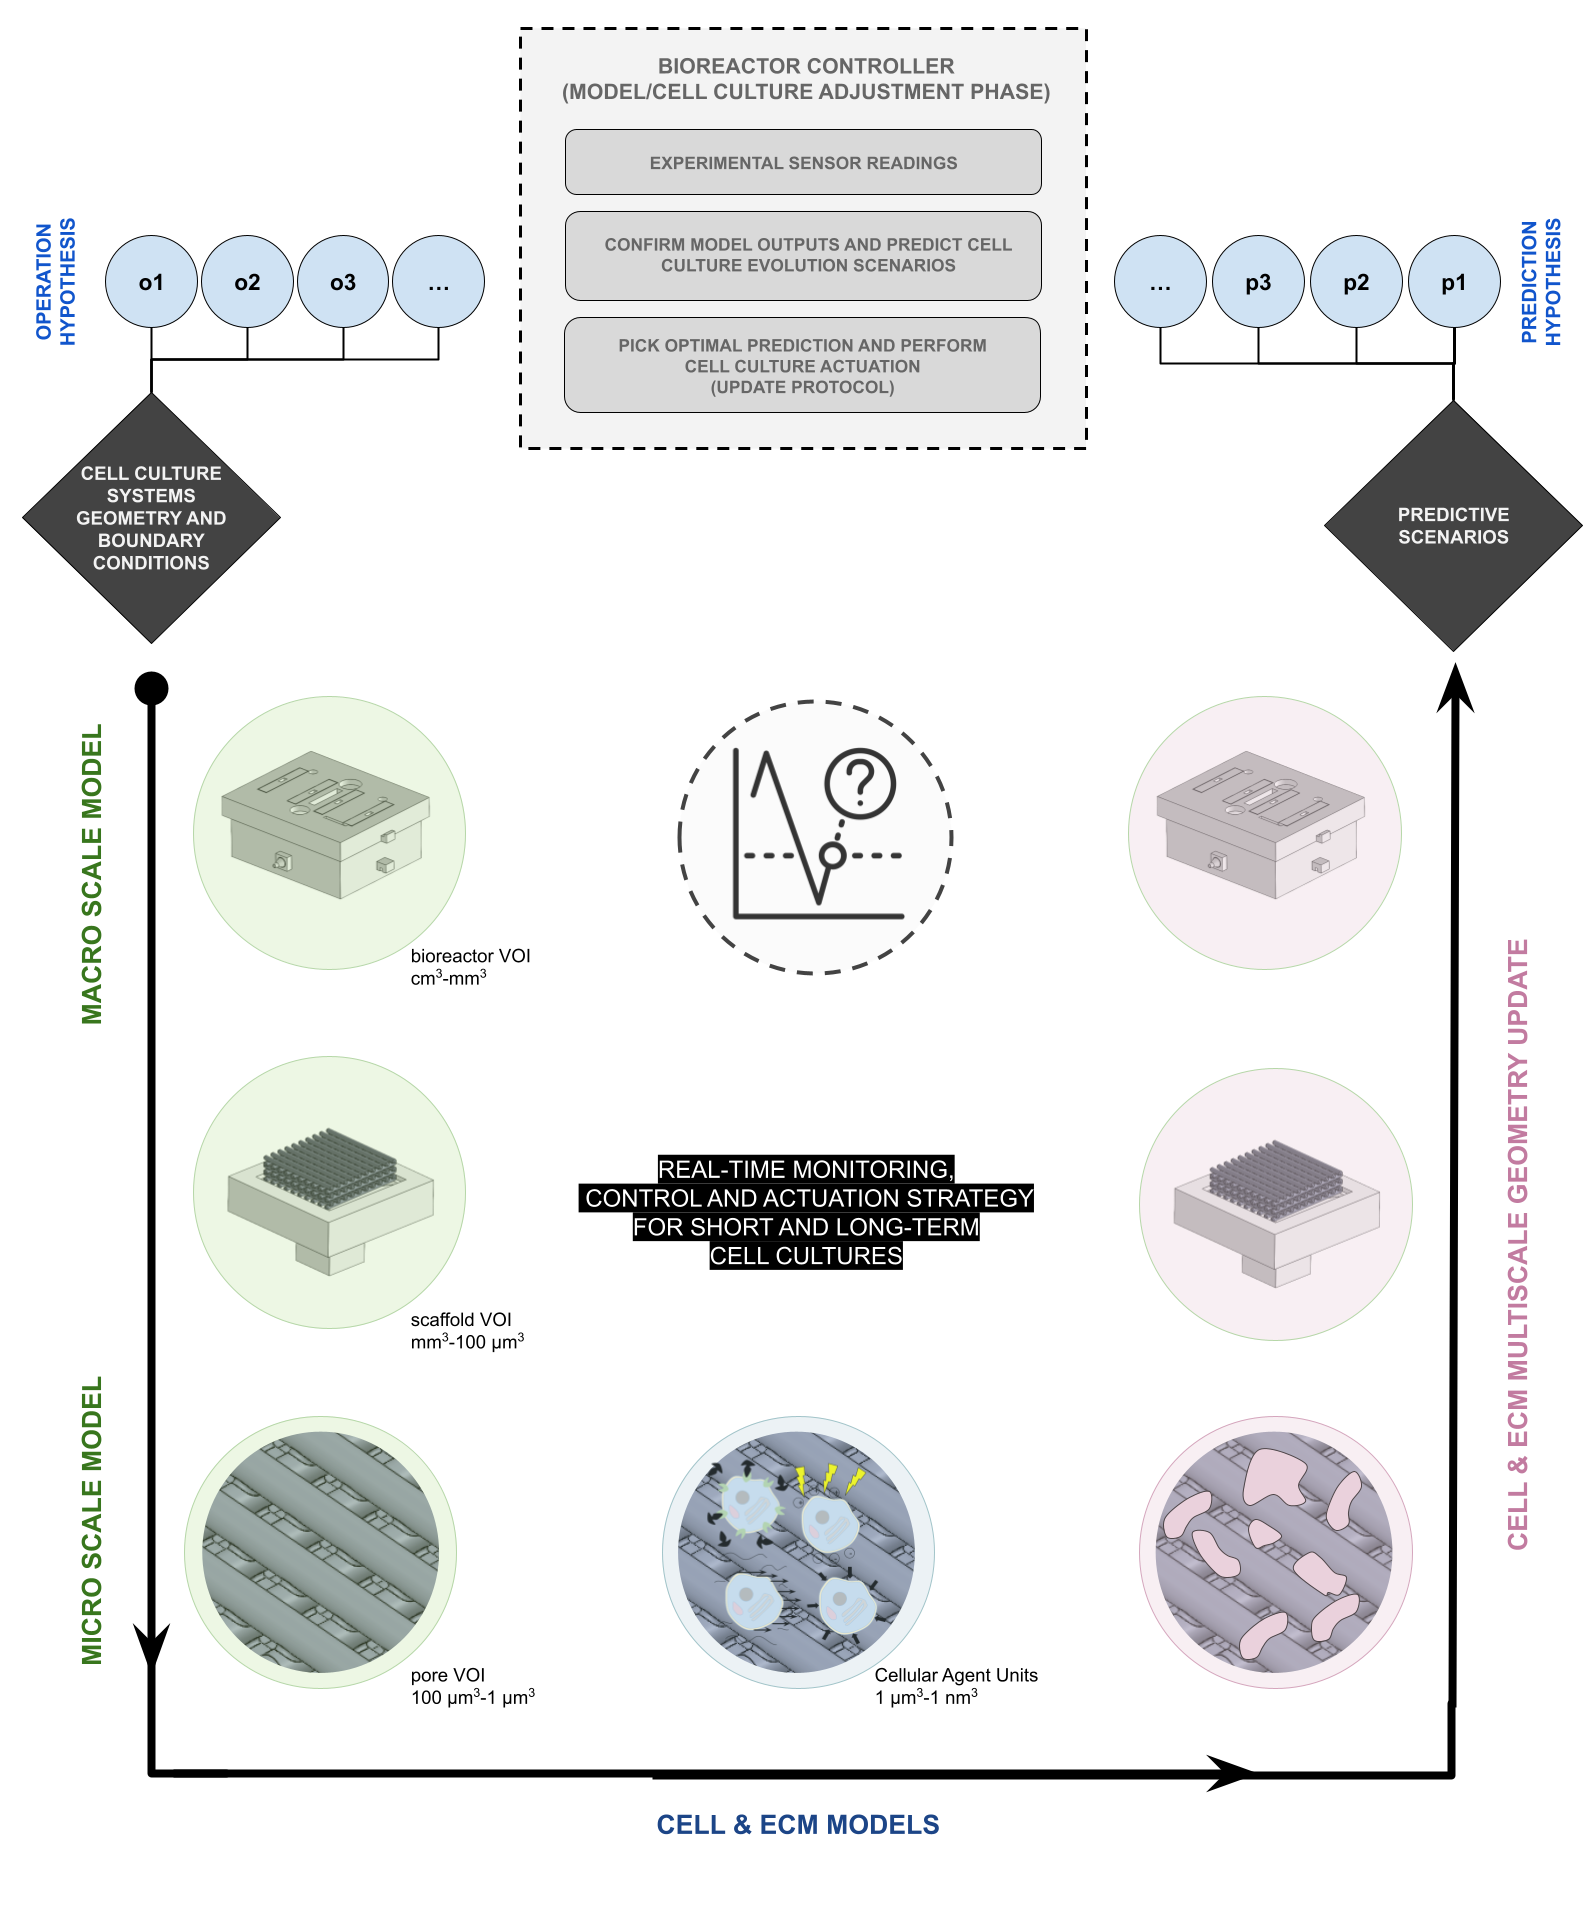
\includegraphics[scale=0.26]{./figures/Figure_7d1}}
\caption{Futuristic concept of the connection between multiscale, multisubject \acs{BTE} / \acs{TE} numerical models and bioreactor monitoring, control, and operation.}
\label{figFuture}
\end{figure}        

The possibility of combining different models, including biology models, will help us to identify the underlying phenomena when comparing the numerical predictions versus the experimental measurements \cite{Geris2018-tz}. Regarding \acs{BTE}, most of the studies so far have focused on mechanics only and neglected the biology \cite{Vetsch2015-xz}. For example, according to the proposed Wolff's Law, bone is deposited and reinforced in areas of greatest stress \cite{Ahn2009-ja}. Despite this law being historically supported from a mechanistic point (by relating physical activity and bone density), a lack of scientific evidence on how this mechanosensory function is performed by bone cells still persists. \textit{In vivo} and \textit{in vitro} numerical modelling of realistic bone conditions, considering strain-generated potentials models (possibly combining bone collagen piezoelectricity and ionic streaming potential) can improve the understanding of how these mechanosensory mechanisms function, while simultaneously assisting experimental setups designs able to recreate the required conditions and protocols to isolate/combine them.

As once stated by P. W. Anderson, a physics Nobel laureate: \enquote{More is Different} \cite{Anderson1972-og}, when referring to the broken symmetry problem, highlighting that the increased hierarchy or specialization of function in a large system, like the ones studied in biology, unexpectedly leads to new rules and processes that arise from the interplay of their simpler parts. Progressively approaching these complex phenomena by bringing different models together may get us one step closer to a new understanding of their underlying reality.  




% VER SE FAZ SENTIDO INCLUIR
%Another interesting experimental observation is made by Rodríguez \textit{et al.} \cite{Fuentes-Rodriguez2022-ey} when placing macroscopic pieces of electric conducting material between immersed parallel plate electrodes. Those, when subjected to the external field polarize throw bipolar induction, generating redox species at the induced poles of opposite charge. The effects observed in these macroscopic metal pieces may be translatable to tissue engineering works when placing conductive scaffolds between electrodes in setups similar to the one applied in this study. Claiming attention to the locally induced effects produced by scaffold material insertion into the stimulation chamber, as predicted previously by our group in a numerical study \cite{Meneses2021-nd}.
%
%Building a clear understanding of DCoupled setups E-Field stimulation and the biophysics of cellular transduction will require a strong electrochemistry characterization of all the materials involved in the electrode/electrolyte interface and in the bulk culture medium region. Several technologies may improve our bioelectrical view of cell behaviour as proposed by \cite{Schofield2020-wz}. Applying currently available bio-electrochemical tools like scanning-ion-conductance (SICM) and scanning-electrochemical-microscopy (SECM) will allow combined mapping of ionic conductivity and redox reactions, respectively, at multiple cell-scale levels, which may unveil the electrical and chemical potential differences across cellular membranes and the electrochemical gradients (ion motive forces) that are effectively being activated by external E-Field stimulation.



%\newpage
%\bibliography{library_c7} 
%\bibliographystyle{plain}
%\end{document}
%\documentclass[11pt]{report}
%\usepackage{siunitx}
%\usepackage{graphicx}
%\usepackage[table,xcdraw]{xcolor}
%\usepackage{csquotes}
%\usepackage{hyperref}
%
%\begin{document}
%\setcounter{chapter}{7}
%\tableofcontents



\newpage
\chapter{Scientific Outputs}
This chapter presents a detailed list of scientific output contributions and communications resulting from this Ph.D. research.
\newpage




\section{Data availability commitment}
Since its beginning, this Ph.D. research has been committed to share designs, precise construction instructions, materials data, tools data, and constructed numerical models. The underlying idea was that, by making these research outputs available to other investigators, the reproducibility and follow-up applications of the developed bioreactor would increase, leading to the adoption and upgrade of the proposed strategy in TE-related areas. Data availability including all mentioned files was achieved through well-established online platforms for scientific data sharing. All the corresponding data links may be found in the respective published manuscript.  


\section{Original research articles}
\begin{enumerate}
\item \small Meneses, João, João C Silva, Sofia R Fernandes, Abhishek Datta, Frederico Castelo Ferreira, Carla Moura, Sandra Amado, Nuno Alves, and Paula Pascoal-Faria. 2020. “A Multimodal Stimulation Cell Culture Bioreactor for Tissue Engineering: A Numerical Modelling Approach”. Polymers 12 (4). DOI: \href{https://doi.org/10.3390/polym12040940}{10.3390/polym12040940}. (SJR: 0.72, IF:5.0, Q1 Chemistry (miscellaneous))
\item \small Meneses, João, Sofia Fernandes, Nuno Alves, Paula Pascoal-Faria, and Pedro Cavaleiro Miranda. 2022. “How to Correctly Estimate the Electric Field in Capacitively Coupled Systems for Tissue Engineering: A Comparative Study”. Scientific Reports 12 (1): 12522. DOI: \href{https://doi.org/10.1038/s41598-022-14834-2}{10.1038/s41598-022-14834-2}. (SJR: 0.97, IF:4.6, Q1 Multidisciplinary)
\item \small João Meneses, Sofia R Fernandes, João C Silva, Frederico Castelo Ferreira, Nuno Alves and Paula Pascoal-Faria. 2023. ''JANUS: an open-source 3D printable perfusion bioreactor and numerical model-based design strategy for tissue engineering''. Front. Bioeng. Biotechnol. 11:1308096. DOI: \href{https://doi.org/10.3389/fbioe.2023.1308096}{10.3389/fbioe.2023.1308096}. (SJR: 0.93, IF:5.7, Q1 Biomedical Engineering)
\item \small João C. Silva \& João Meneses, Fábio F.F. Garrudo, Sofia R. Fernandes, Nuno Alves, Frederico Castelo Ferreira, Paula Pascoal-Faria. ''Direct coupled electrical stimulation towards improved osteogenic differentiation of human mesenchymal stem/stromal cells: a comparative study of different protocols'' (Under Revision at Nature Scientific Reports - SJR: 0.97, IF:4.6, Q1 Multidisciplinary)
\end{enumerate}


\section{Conference Proceedings}
\begin{enumerate}
\item \small Meneses, Joao, Sofia R. Fernandes, Nuno Alves, Paula Pascoal-Faria, and Pedro Cavaleiro Miranda. 2021. “Effects of Scaffold Electrical Properties on Electric Field Delivery in Bioreactors.” Conference Proceedings: Annual International Conference of the IEEE Engineering in Medicine and Biology Society. IEEE Engineering in Medicine and Biology Society. (November): 4147–51. DOI: \href{https://doi.org/10.1109/EMBC46164.2021.9630711}{10.1109/EMBC46164.2021.9630711}
\item \small João Meneses, Carla Moura, Abhisked Datta, Pedro Cavaleiro Miranda, Nuno Alves, Paula Pascoal-Faria. 2021
“The influence of scaffold design in electrical field distribution for tissue engineering.'' Conference Proceedings: The 19th International Conference of Numerical Analysis and Applied Mathematics, Rhodes, Greece.
\item \small Meneses, Joao, Sofia R. Fernandes, Abhishek Datta, Sandra Amado, Nuno Alves, and Paula Pascoal-Faria. 2022. “Numerical Modelling of a Bioreactor Design Targeting Optimal Conditions for Cell Culture.” AIP Conference Proceedings 2425 (1): 220003. DOI: \href{https://doi.org/10.1063/5.0081336}{10.1063/5.0081336}.
\item \small Fernandes, Sofia R., João Meneses, Abhishek Datta, Sandra Amado, Nuno Alves, and Paula Pascoal-Faria. 2022. “Comparison of Electromagnetic Stimulation Fields Generated by Different Experimental Setups: A Biophysical Analysis.” AIP Conference Proceedings 2425 (1): 220004. DOI: \href{https://doi.org/10.1063/5.0081338}{10.1063/5.0081338}.
\end{enumerate}


\section{Oral Presentations}
\begin{enumerate}
\item \small João Meneses, Nuno Alves, Paula Pascoal-Faria. "Electrical Stimulation of Bioscaffolds for Tissue Engineering: a Numerical Analysis" presented at 17\textsuperscript{th} International Conference of Numerical Analysis and Applied Mathematics, held online and presential at Rhodes, Greece, 23-28 September 2019;
\item \small João Meneses, Nuno Alves, Sofia R. Fernandes, Carla Moura, Abhishek Datta, Sandra Amado, P C Miranda, Paula Pascoal-Faria. ''Numerical Modelling of Multi-Coupling Electrodes and Bioreactor Combined System for Electric Stimulation in Tissue Engineering.'' presented at RESIM 2020 / BIODIG 2020 conference held in Centre for Rapid and Sustainable Product Development, Polytechnic Institute of Leiria, 5 June 2020;
\item \small João Meneses, Abhisked Datta, Nuno Alves, Pedro Cavaleiro Miranda and Paula Pascoal-Faria. "Bioreactor Design Challenges and Opportunities: Combining Direct Digital Manufacturing and Numerical Models" presented at ICDDMAP 2021, Session C -Mathematics and Industry, held online, organized by the Centre for Rapid and Sustainable Product Development, Polytechnic Institute of Leiria, and Karnatak University, Dharwad, India. Awarded as Best Presentation in Session C;
\item \small João Meneses, Abhisked Datta, Nuno Alves and Paula Pascoal-Faria. "From Numerical Models to Bioreactor Design in Tissue Engineering" presented at Encontro Nacional da Sociedade Portuguesa de Matemática 2021 (ENSPM 2021), held online, 12-16 July 2021;
\item \small João Meneses, João Silva, Nuno Alves, Tiago Santos, Pedro Cavaleiro Miranda, Paula Pascoal-Faria. “Bioreactor Digital Twin - An essential modelling tool to estimate cellular local environmental conditions in experimental tissue engineering;” presented at International Conference on Computational Bioengineering (ICCB2022), held at Instituto Superior Técnico, Lisbon, Portugal, 11 - 13 April 2022;
\item \small João Meneses, João Silva, Nuno Alves, Tiago Santos, Pedro Cavaleiro Miranda, Paula Pascoal-Faria. “Numerical Modelling Impact in the Design and Operation of Tissue Engineering Systems.” presented at Afternoon Session D - Numerical modelling of the manufacturing of complex systems, RESIM 2022 / BIODIG 2022 conference held in Centre for Rapid and Sustainable Product Development, Polytechnic Institute of Leiria, 3 June 2022;
\item \small João Meneses, Nuno Alves, Pedro Cavaleiro Miranda, Paula Pascoal-Faria. ''Mechanical and EMS in Tissue Engineering. Open Source Bioreactor + Digital Twin Solution.'' Invited lecturer for a weekly research digest at Instituto Superior Técnico, 12 July 2022;
\item \small João Meneses, Sofia R. Fernandes, Nuno Alves, Paula Pascoal-Faria. ''Janus Bioreactor Methodology - A shareable and replicable design for a perfusion bioreactor: decisions on 3D printing supported by a numerical modelling framework.'' presented at Tissue Engineering and Regenerative Medicine International Society (TERMIS) European Chapter Meeting 2023 held in Manchester on the 28th to 31st March 2023. 
\end{enumerate}


\section{Posters}
\begin{enumerate}
\item \small Meneses, João; João C. Silva; Sofia R. Fernandes; Abhishek Datta; Frederico Castelo Ferreira; Carla Moura;
Sandra Amado. "How to improve Tissue Engineering bioreactor solutions to deliver accurate and replicable electromagnetic (EMS) and mechanical stimulation?". Work presented at Ciências Research Day 2020, FCUL, Lisbon, Portugal;
\item \small Meneses, João; João C. Silva; Sofia R. Fernandes; Abhishek Datta; Frederico Castelo Ferreira; Carla Moura;
Sandra Amado."Bioreactor Design: Combining Direct Digital Manufacturing and Numerical Models". Work presented at the Ciência 2021 - Science and Technology in Portugal Summit, 28-30 June 2021, which took place at the Lisbon Congress Centre, Portugal;
\item \small João Meneses, Nuno Alves, Paula Pascoal-Faria, Pedro Cavaleiro Miranda. “Multiscale Numerical Models for Tissue Engineering Applications.” presented at the Jornadas Doutorais, February 2022, which took place at FCUL, Lisbon, Portugal;
\item \small João Meneses, Sofia R. Fernandes, Nuno Alves, Paula Pascoal-Faria. ''Janus Bioreactor - An open-source concept that combines a 3D printable bioreactor with its numerical models, a strategy that may help to improve bioreactor design, operation, control, and overall scientific repeatability.'' presented at Jornadas Doutorais, February 2023, which took place at FCUL, Lisbon, Portugal;
\end{enumerate}


\section{Collaborations}
\begin{enumerate}
\item \small Mateus, J. C., Cdf Lopes, M. Aroso, A. R. Costa, A. Gerós, J. Meneses, P. Faria, et al. 2021. “Bidirectional Flow of Action Potentials in Axons Drives Activity Dynamics in Neuronal Cultures.” Journal of Neural Engineering 18 (6). DOI: \href{https://doi.org/10.1088/1741-2552/ac41db}{10.1088/1741-2552/ac41db};
\item \small Marcelino, Pedro, João Carlos Silva, Carla S. Moura, João Meneses, Rachel Cordeiro, Nuno Alves, Paula Pascoal-Faria, and Frederico Castelo Ferreira. 2023. “A Novel Approach for Design and Manufacturing of Curvature-Featuring Scaffolds for Osteochondral Repair.” Polymers 15 (9). DOI: \href{https://doi.org/10.3390/polym15092129}{10.3390/polym15092129};
\item \small João C. Silva, Pedro Marcelino, João Meneses, Frederico Barbosa, Carla S. Moura,e Ana C. Marques, Joaquim M. S. Cabral, Paula Pascoal-Faria, Nuno Alves, Jorge Morgado, Frederico C. Ferreira, Fábio F. F. Garrudo. ''Synergy between 3D-extruded electroconductive scaffolds and electrical stimulation in enhancing bone regeneration''. (Under Submission at RCS Journal of Materials Chemistry);
\end{enumerate}



%\end{document}

% Referências
\newpage
\bibliography{library_global} 
\bibliographystyle{unsrt}

\end{document}